% ------------------------------------------------------------------------
% -*-TeX-*- -*-Hard-*- Smart Wrapping
% ------------------------------------------------------------------------
% AMS-LaTeX definitions:     Thesis ++++ Alex, September 1994 ************
% ------------------------------------------------------------------------
% Ph.D. Thesis Defended on November 25, 1994
% ------------------------------------------------------------------------
\documentclass[12pt]{report}
\usepackage{graphicx}
%\usepackage{graphicx,float,subfigure,hyperref,pgf,tikz,mathrsfs,dblfloatfix}
\usepackage{hyperref}
\hypersetup{
	colorlinks=true,
	linkcolor=blue,
	citecolor=blue %[rgb]{0.4,0.4,0.4}
}
\usepackage{epigraph}

% \epigraphsize{\small}% Default
\setlength\epigraphwidth{8cm}
\setlength\epigraphrule{0pt}
\usepackage{etoolbox}
\makeatletter
\patchcmd{\epigraph}{\@epitext{#1}}{\itshape\@epitext{#1}}{}{}
\makeatother

\usepackage{float}
\usepackage[nice]{nicefrac}
\usepackage{geometry}
%\usepackage[left=2.5cm,top=3cm,right=3cm,bottom=3cm,bindingoffset=0.0cm]{geometry}
\usepackage[centertags]{amsmath}
%\usepackage[T1]{fontenc}
%\usepackage{mathptmx}
\usepackage{tabto}
\usepackage{color}
\usepackage{amsfonts}
\usepackage{amssymb}
\usepackage{subfigure}
\usepackage{amsthm}
\usepackage{multirow}
\usepackage{booktabs}
\usepackage{algorithm}
\usepackage[noend]{algpseudocode}
\usepackage{adjustbox,lipsum}
\usepackage{pgf}
\usepackage{rotating}
%\usepackage[font=footnotesize]{caption}
%\usepackage[font=footnotesize]{subcaption}
%\usepackage[cmex10]{amsmath}
\usepackage{newlfont}
\usepackage{enumitem}
\usepackage{natbib} %bib package for citep
\usepackage{XThesis} %DAL Thesis Style
\usepackage{XTocinc} %Include Table of Contents as the first entry in TOC
%                     Faculty of Grad Studies insists on this!?
%\usepackage[active]{srcltx}  %SRC Specials for DVI search
% Fuzz -------------------------------------------------------------------
\hfuzz2pt % Don't bother to report over-full boxes if over-edge is < 2pt
% Line spacing -----------------------------------------------------------
\newlength{\defbaselineskip}
\setlength{\defbaselineskip}{\baselineskip}
\newcommand{\setlinespacing}[1]%
           {\setlength{\baselineskip}{#1 \defbaselineskip}}
\newcommand{\doublespacing}{\setlength{\baselineskip}%
                           {2.0 \defbaselineskip}}
\newcommand{\singlespacing}{\setlength{\baselineskip}{\defbaselineskip}}
\newcommand{\ra}[1]{\renewcommand{\arraystretch}{#1}}
% MATH -------------------------------------------------------------------
\newcommand{\A}{{\cal A}}
\newcommand{\h}{{\cal H}}
\newcommand{\s}{{\cal S}}
\newcommand{\W}{{\cal W}}
\newcommand{\BH}{\mathbf B(\cal H)}
\newcommand{\KH}{\cal  K(\cal H)}
\newcommand{\Real}{\mathbb R}
\newcommand{\Complex}{\mathbb C}
\newcommand{\Field}{\mathbb F}
\newcommand{\RPlus}{[0,\infty)}
%
% My macros
\newcommand{\note}[1]{\textcolor{red}{#1}}
%\newcommand{\x}{\ensuremath{x}}
\newcommand{\y}{\ensuremath{y}}

\newcommand{\norm}[1]{\left\Vert#1\right\Vert}
\newcommand{\essnorm}[1]{\norm{#1}_{\text{\rm\normalshape ess}}}
\newcommand{\abs}[1]{\left\vert#1\right\vert}
\newcommand{\set}[1]{\left\{#1\right\}}
\newcommand{\seq}[1]{\left<#1\right>}
\newcommand{\eps}{\varepsilon}
\newcommand{\To}{\longrightarrow}
\newcommand{\RE}{\operatorname{Re}}
\newcommand{\IM}{\operatorname{Im}}
\newcommand{\Poly}{{\cal{P}}(E)}
\newcommand{\EssD}{{\cal{D}}}



\newcommand{\X}{\ensuremath{X}} % Trial signal matrix (training) :				X
\newcommand{\onlineX}{\ensuremath{\chi}} % Trial signal matrix (training) :		X
\newcommand{\Y}{\ensuremath{Y}} % Trial signal matrix (test): 						Y
\newcommand{\totd}{\ensuremath{{m}}} % dimension of the manifold : 				m
\newcommand{\chI}{\ensuremath{c}} %channel or channel index: 					c
\newcommand{\dc}{\ensuremath{C}} % dimension nb of electrode : 					C
\newcommand{\si}{\ensuremath{n}} %sample or sample index: 							n
\newcommand{\dt}{\ensuremath{N}} % dimension nb of samples (trial length):		N
\newcommand{\dr}{\ensuremath{\mathcal{N}}} % recording length:						N
\newcommand{\nb}{\ensuremath{i}} %index of a number : 								i
\newcommand{\Nb}{\ensuremath{I}} %a number of objects : 							I
\newcommand{\ci}{\ensuremath{k}} %class or class index: 							k
\newcommand{\dK}{\ensuremath{K}} %nb classes for SSVEP:	              K
\newcommand{\df}{\ensuremath{f}} %frequency SSVEP index:	            f
\newcommand{\dF}{\ensuremath{F}} %dimension nb of frequencies for SSVEP:	F
\newcommand{\ti}{\ensuremath{i}} %trial or trial index: 							i
\newcommand{\dT}{\ensuremath{I}} %dimension nb of trials : 						I
\newcommand{\setindex}{\ensuremath{\mathcal{I}}} %Set of indeces of trials corresponding to a specific class I
\newcommand{\dd}{\ensuremath{D}} %dimension nb of segment(epochs) for classif: 	D
\newcommand{\tj}{\ensuremath{j}} %trial or trial index: 							j
\newcommand{\Dindex}{\ensuremath{\mathcal{J}}} %Set of indeces within the last \dd segments (epoch) 
\newcommand{\fpnorm}{\ensuremath{p}} %fixed pont normalisation factor :			p
\newcommand{\cue}{\ensuremath{\tau_0}} %Cue on set time:							tau
\newcommand{\deltaN}{\ensuremath{\Delta \si}} % Sliding step size 
\newcommand{\ws}{\ensuremath{w}} % Sliding window size							w
%------------------------------------------------------------------------------
\newcommand{\w}{\ensuremath{\mathbf{w}}} % bold w (filter)							w
\newcommand{\m}{\ensuremath{\mathbf{m}}}	%						bold				m 
\newcommand{\scat}{\ensuremath{\tilde{s}^2}}
\newcommand{\Scat}{\ensuremath{\mathbf{\Sigma}}}
\newcommand{\Yc}{\ensuremath{\mathcal{Y}}}
\newcommand{\Xc}{\ensuremath{\mathcal{X}}}
\newcommand{\dotSpace}{\ensuremath{\mathcal{H}}}
\newcommand{\inputSpace}{\ensuremath{\mathcal{X}}}
\newcommand{\xfilt}{\ensuremath{\mathbf{u}}} %			xdawn filter
\newcommand{\ssnr}{\ensuremath{\rho}}

\newcommand{\di}{\ensuremath{d}} % Sliding segment(epoch) index							d
\newcommand{\Xs}[1] {\ensuremath{\X_{\operatorname{\text{#1}}}}} % Sliding EEG Segment(epoch)
\newcommand{\Xsig}{\ensuremath{\overrightarrow{\X}}}
\newcommand{\GenMa}{\ensuremath{\mathcal{M}}} %generic manifold M
\newcommand{\Ma}{\ensuremath{\mathcal{M}_{\dc}}} % Riemannian manifold of SPD matrices
\newcommand{\Sy}{\ensuremath{\mathcal{S}_{\dc}}} % Euclidean space of symmetric matrices
\renewcommand{\P}{\ensuremath{\Sigma}} % A point of the Riemannian manifold, was P
\renewcommand{\S}{\ensuremath{\Theta}} % A point of the tangent space, was S
\newcommand{\ev}{\ensuremath{\lambda}} % an eigenvector
\newcommand{\distF}{\ensuremath{d_{\operatorname{E}}}} % Frobenius metric
\newcommand{\distR}{\ensuremath{\delta}} % Riemannian metric
\newcommand{\distLE}{\ensuremath{d_{\operatorname{LE}}}} % LogEuclidean distance
\newcommand{\distH}{\ensuremath{d_{\operatorname{H}}}}
\newcommand{\distW}{\ensuremath{d_{\operatorname{W}}}}
\newcommand{\distAIRM}{\ensuremath{d_{\operatorname{AI}}}} % Affine invariant Riemannian metric distance
\newcommand{\distB}{\ensuremath{d_{\operatorname{B}}}} % Log Det distance
\newcommand{\distAD}{\ensuremath{d_{\alpha\operatorname{D}}}} % Log Det distance
\newcommand{\dist}{\ensuremath{d}} % distance (metric)		d
\newcommand{\Pm}{\ensuremath{\bar{\P}}} % Karcher Mean of Matrices
\newcommand{\PmE}{\ensuremath{\bar{\P}_{\operatorname{E}}}} % Euclidean Mean of Matrices
\newcommand{\PmLE}{\ensuremath{\bar{\P}_{\operatorname{LE}}}} % LogEuclidean Mean of Matrices
\newcommand{\PmKL}{\ensuremath{\bar{\P}_{\operatorname{KL}}}} % KL Mean of Matrices
\newcommand{\PmAIRM}{\ensuremath{\bar{\P}_{\operatorname{AI}}}} % AIRM Mean of Matrices
\newcommand{\PmB}{\ensuremath{\bar{\P}_{\operatorname{B}}}} % LogDet Mean of Matrices
\newcommand{\PmAD}{\ensuremath{\bar{\P}_{\alpha\operatorname{d}}}} % LogDet Mean of Matrices
\newcommand{\PmH}{\ensuremath{\bar{\P}_{\operatorname{H}}}} % Euclidean Mean of Matrices
\newcommand{\metric}{\ensuremath{\mathit{d}}} % Riemannian metric		d
\newcommand{\divB}[1]{\ensuremath{D_{\operatorname{#1}}}}
\newcommand{\tr}{\ensuremath{\operatorname{tr}}}
\newcommand{\mdrmpotato}{MDRM-Potato}
\newcommand{\onlinepotato}{Online-Potato}

\newcommand{\Rm}{\ensuremath{\mu}} % Riemannian mean
\newcommand{\EX}{\ensuremath{\omega}} % Expected vector of \X
\newcommand{\tarco}{\ensuremath{\Gamma}} % target covariance in shrinkage estimator
\newcommand{\mle}{\ensuremath{\hat{\ell}}} % maximum likelihood estimator of fixed point cov
\newcommand{\fmle}{\ensuremath{g}} % function of fixed point cov MLE
\newcommand{\supertrial}{\ensuremath{Z}} % super-trial signal of Barachant.
\newcommand{\pocc}{\ensuremath{\rho}} % occurence probability for classification 
\newcommand{\pthres}{\ensuremath{\vartheta}} % probability threshold for classification

\newcommand{\clout}{\ensuremath{\ci^*}} % class output from classification algo 1  :f*
\newcommand{\cloutOn}{\ensuremath{\tilde{\ci}}} % class output from classification algo 2  :~f
\newcommand{\cloutmp}{\ensuremath{\bar{\ci}}} % class output from classification algo 2  :f**
\newcommand{\clarray}{\ensuremath{\mathcal{K}}} % class output from classification algo 2  :~f

% \newcommand{\mle}{\ensuremath{\hat{\mathbf{M}}}}
%\newcommand{\SCM}{\ensuremath{\mathbf{S}}}
% \newcommand{\Po}{\ensuremath{\mathcal{P}}} no need, use \Ma instead
%\newcommand{\Rm}{\ensuremath{\mathfrak{G}}} % I prefer to avoid German char
\newcommand{\x}{\ensuremath{x}} % I prefer non-bold notations for vectors
\newcommand{\xb}{\ensuremath{\bar{x}}}
% \newcommand{\x}{\ensuremath{\mathbf{x}}}
% \newcommand{\xb}{\ensuremath{\bar{x}}}}
% \newcommand{\eye}{\ensuremath{\mathbbm{I}}}
\newcommand{\eye}{\ensuremath{\mathbf{I}}}
%\newcommand{\unitary}{\ensuremath{\mathbbm{1}}}
\newcommand{\unitary}{\ensuremath{\mathbf{1}}}
\newcommand{\argmin}{\arg\!\min}
%\newcommand{\argmax}{\arg\!\max}
\DeclareMathOperator*{\argmax}{arg\,max}
\renewcommand{\Re}{\ensuremath{\mathbb{R}}}
\newcommand{\Log}[1]{\ensuremath{\operatorname{Log}_{#1}}}
\newcommand{\Exp}[1]{\ensuremath{\operatorname{Exp}_{#1}}}
\newcommand{\Expm}{\ensuremath{\operatorname{Exp}}}
\newcommand{\Logm}{\ensuremath{\operatorname{Log}}}
\newcommand{\cov}[1]{\ensuremath{\hat{\Sigma}_{\operatorname{#1}}}}
\newcommand{\disvec}{\ensuremath{\widetilde{\delta}}} %\vec{\delta}}}
\newcommand{\diffdist}{\ensuremath{\delta}}  % \pmb{\delta}}}
\newcommand{\zs}{\ensuremath{\mathit{z}}} % Sliding window size

\newcommand{\Dtr}{\ensuremath{\mathcal{D}}} 
\newcommand{\Ttr}{\ensuremath{\mathcal{T}}} 
\newcommand{\ftr}{\ensuremath{\mathit{f}}}
\newcommand{\Xtr}{\ensuremath{\mathcal{X}}}
\newcommand{\Ytr}{\ensuremath{\mathcal{Y}}} 

\newcommand{\simil}{\ensuremath{\mathtt{s}}} 		% Similarity between two subjects
\newcommand{\kld}{\ensuremath{\text{KL}_D}}		% Kullback Leibler divergence
\newcommand{\cm}{\ensuremath{\mathbf{C}_c}}		% Class mean
\newcommand{\ccm}{\ensuremath{\mathfrak{C}_c}}		% Composite class mean
% THEOREMS ---------------------------------------------------------------
\theoremstyle{plain}
\newtheorem{thm}{Theorem}[section]
\newtheorem{cor}[thm]{Corollary}
\newtheorem{lem}[thm]{Lemma}
\newtheorem{prop}[thm]{Proposition}
%
\theoremstyle{definition}
\newtheorem{defn}{Definition}[section]
%\newtheorem{defn}[thm]{Definition} 
%
\theoremstyle{remark}
\newtheorem{rem}{Remark}[section]
%
\numberwithin{equation}{section}
\renewcommand{\theequation}{\thesection.\arabic{equation}}
%%% ----------------------------------------------------------------------

\setlength{\tclineskip}{1.05\baselineskip}
%%% ----------------------------------------------------------------------
\setcitestyle{square}
%\nobib
%\draft
%\nofront

%\permissionfalse

%\dedicate{To my loving parents, Alphonsine and Justin Kalunga, to my brother and sisters.\\
%Your love, patience, and care have always accompanied me}

\nolistoftables
\nolistoffigures
%\dtech
\phd
%\copyrightyear{1994}
\submitdate{July, 2016}
\date{21 Octobre 2016}
%\convocation{May}{1995}

% ------------------------------------------------------------------------

\title{Toward User-adapted Brain Computer Interfaces: Robust Interaction and Machine Learning based on Riemannian Geometry}
%
\author{Emmanuel K. Kalunga}
%
\supervisor{\\Karim Djouani - Professor\\Eric Monacelli - Associate Professor }
%
\cosupervisor{\\Sylvain Chevallier - Associate Professor \\ Yskandar Hamam - Professor }
%

%
\dept{Sciences et Technologies de l'Information et de la Communication}
%
\field{Computer Science}
%
\university{Universit\'{e} Paris-Saclay, UVSQ}

\degrees{Doctor Technologiae} 
\degreeinitials{D-Tech}
\fields{Electrical Engineering}
\faculty{Faculty of Engineering and the Built Environment}
\universitys{Tshwane University of Technology}
% ------------------------------------------------------------------------

\begin{document}
%{
\typeout{:?000000000} % Don't bother with over/under-full boxes
\beforepreface
\typeout{:?111111111} % Process All Errors from Here on
%}
% --------------------------------------------------------------------------
%\setcounter{page}{1}
%\tableofcontents

%% ------------------------------------------------------------------------
%{ \typeout{Acknowledgements}
%% ------------------------------------------------------------------------
% -*-TeX-*- -*-Hard-*- Smart Wrapping
% ------------------------------------------------------------------------
% Thesis Acknowledgements ------------------------------------------------

\addtolength{\topmargin}{-.875in}

\prefacesection{Acknowledgements}
%\def\baselinestretch{1.0}
\setlinespacing{1.66}

\medskip
\par
I would like to thank my supervisors Prof Karim Djouani and Prof Yskandar
Hamam for their guidance and support. From the very beginning, their
experience and wisdom have been instrumental for the completion of this work.

\medskip

My gratitude to Tshwane University of Technology (TUT) and the French South
African Institute of Technology (F'SATI) for providing a suitable research
environment. My gratitude is particularly extended to Dr Anish Kurien, for
his support and constructive advice.

\medskip

I am profoundly thankful to the \emph{Laboratoire d'Ing\'{e}nierie des
Syst\`{e}mes de Versailles} (LISV) for providing the necessary research
material and environment for the experiments conducted. A special word of
thanks to Prof Eric Monacelli, Prof Sylvain Chevallier, and Dr Zoran Tiganj.
They have made my stay in the laboratory a success, and this work could not
have been possible without their assistance.

\medskip

I express my sincere gratitude to the Mandela-Rhodes Foundation (MRF) for its
financial support throughout my entire masters studies. When I had to join
the LISV, the Foundation did not hesitate to support the ticket fare from
South Africa to France and back.

% ----------------------------------------------------------------------

%}
%% ------------------------------------------------------------------------
%{
\typeout{Abstract}
		% ------------------------------------------------------------------------
% -*-TeX-*- -*-Hard-*- Smart Wrapping
% ------------------------------------------------------------------------
% Thesis Abstract --------------------------------------------------------

% \addtolength{\topmargin}{-1.6in}
% \addtolength{\textheight}{1.6in}

\prefacesection{Abstract}

In the last two decades, interest in Brain-Computer Interfaces (BCI) has tremendously grown, with a number of research laboratories working on the topic. 
Since the \emph{Brain-Computer Interface Project} of Vidal in 1973, where BCI was introduced for rehabilitative and assistive purposes, the use of BCI has been extended to more applications such as neurofeedback and entertainment.
The credit of this progress should be granted to an improved understanding of electroencephalography (EEG), an improvement in its measurement techniques, and increased computational power. 

Despite the opportunities and potential of Brain-Computer Interface, the technology has yet to reach maturity and be used out of laboratories. 
There are several challenges that need to be addresses before BCI systems can be used to their full potential.
This work examines in depth some of these challenges, namely the specificity of BCI systems to users physical abilities, the robustness of EEG representation and machine learning, and the adequacy of training data.
The aim is to provide a BCI system that can adapt to individual users in terms of their physical abilities/disabilities, and variability in recorded brain signals. 
%Variabilities in recorded brain signals are due to differences in users brain anatomies, neuronal responses, as well as random noise in the experimental environment.

To this end, two main avenues are explored: the first, which can be regarded as a high-level adjustment, is a change in BCI paradigms. 
It is about creating new paradigms that increase their performance, ease the discomfort of using BCI systems, and adapt to the user's needs.
The second avenue, regarded as a low-level solution, is the refinement of signal processing and machine learning techniques to enhance the EEG signal quality, pattern recognition and classification.   

On the one hand, a new methodology in the context of assistive robotics is defined: it is a hybrid approach where a physical interface is complemented by a Brain-Computer Interface (BCI) for human machine interaction.
This hybrid system makes use of user’s residual motor abilities and offers BCI as an optional choice: the user can choose when to rely on BCI and could alternate between the muscular- and brain-mediated interface at the appropriate time. 
 
%The concept is demonstrated for patients with degenerative diseases that affect large muscles but spare the wrists and hands motor capacities. An adapted 3D touchless interface is used for continuous control and a steady-state visually evoked potential (SSVEP)-based BCI for triggering specific actions. 
%While the touchless interface allows the subject to use their residual motor abilities, the SSVEP-based BCI with state-of-the-art signal processing and machine learning~\citep{kalunga_ssvep_2013} is able to provide timely intervention for a better control in a multimodal setup. Experimentaly, the concept is evaluated for navigation in a virtual environment and in the control of a robotic arm exoskeleton designed to compensate for muscular dystrophy in the shoulder and elbow muscles occurring in our subjects of interest~\citep{kalunga_hybrid_2014}.

On the other hand, for the refinement of signal processing and machine learning techniques, this work uses a Riemannian framework.
A major limitation in this filed is the EEG poor spatial resolution. 
This limitation is due to the volume conduction effect, as the skull bones act as a non-linear low pass filter, mixing the brain source signals and thus reducing the signal-to-noise ratio. 
Consequently, spatial filtering methods have been developed or adapted. 
Most of them (i.e. Common Spatial Pattern, xDAWN, and Canonical Correlation Analysis) are based on covariance matrix estimations. 
The covariance matrices are key in the representation of information contained in the EEG signal and constitute an important feature in their classification.
In most of the existing machine learning algorithms, covariance matrices are treated as elements of the Euclidean space. 
However, being Symmetric and Positive-Definite (SPD), covariance matrices lie on a curved space that is identified as a Riemannian manifold. 
Using covariance matrices as features for classification of EEG signals and handling them with the tools provided by Riemannian geometry provide a robust framework for EEG representation and learning. 

%#####################################################################################################
% ----------------------------------------------------------------------

%}

%\tableofcontents
% ---------------------------------------------------------------------------
\afterpreface
%% ------------------------------------------------------------------------
%{ \typeout{Definitions}
%\include{GLOS}
\pagenumbering{arabic}
%}
\def\baselinestretch{1}
\setlinespacing{1.2}
%\setlinespacing{1.25}

%\addtolength{\topmargin}{-.975in}
%\addtolength{\textheight}{-.1in}

% ------------------------------------------------------------------------
%{
\typeout{Introduction}
% ------------------------------------------------------------------------
% -*-TeX-*- -*-Hard-*- Smart Wrapping
% ------------------------------------------------------------------------
%%% Thesis Introduction --------------------------------------------------

%\addtolength{\topmargin}{-.875in}
%\addtolength{\textheight}{.875in}
%\footskip
%\nonumchapter{Introduction}

\chapter{Introduction}
\label{chap:intro}
\epigraph{The only way of discovering the limits of the possible is to venture a little way past them into the impossible.}{--- \textup{ Arthur C. Clarke}, Profiles of the Future: An Enquiry into the Limits of the Possible}

This chapter follows the structure of the Tshwane University of Technology's theses. It is an introductory chapter that lays out the background of the research field, states the research problem and objective, and summarises the contribution brought by this work to the research filed.   
\section{Background}% and justification

%This should be a quick overview of BCI with the following points:
%1) Definition and Objective of BCI
%2) Quick Description of a BCI components
%3) Quick history of BCI (measure events and turning points in BCI research)
%4) The current state of the art (generally what can be achieved by BCI technology, where we currently stand in the research without insiting on the limitations. 
%5) BCI types -> mention them and their pros and cons
%6) Usability of BCI (practical use, BCI illiteracy)
%7) Signal processing: Machine learning pipeline => Cov mat => Riemannian => Training sample size vs. Feature space (curse of dimensionality)
%References:
%- Brain–computer interfaces in neurological rehabilitation, Janis J Daly and Jonathan R Wolpaw 2008
%- Combining brain–computer interfaces and assistive technologies: state-of-the-art and challenges, J. d. R. Millán et al. 2010
%- Brain Computer Interfaces, a Review. Luis Fernando Nicolas-Alonso and Jaime Gomez-Gil 2012
Brain-computer interfaces (BCI) also called brain machine interfaces (BMI) are devices that translates measured brain activity into tangible actions, allowing humans and apes to interact with the physical environment without using their muscular system.
In the last two decades, interest in brain-computer interfaces has tremendously grown, with a number of research laboratories working on the topic. 
Since the \emph{Brain-Computer Interface Project}~\citep{vidal_toward_1973}, joint effort from researchers in electronics, neuroscience, electrical engineering, signal processing, and machine learning -- to name but a few, has promoted the use of BCI in different applications such as neurofeedback, entertainment, and assistance. 
Better understanding, improved measurement and processing of electroencephalograms (EEG) are at the centre of the growth of non-invasive EEG based BCI. 
These interfaces have brought a complete paradigm shift to assistive technologies. 
In fact, unlike traditional human machine interfaces, BCI do not rely on motor abilities. 
Bypassing the neuromuscular pathways, BCI constitutes a golden opportunity for people with limited neuromuscular abilities or serious brain injuries. Brain-computer interfaces can be used for control or communication in replacement of traditional assistive devices~\citep{wolpaw_brain-computer_2002}, or for improved human-machine interaction as a passive user feedback to the machine~\citep{zander_towards_2011}.

BCI systems rely on neurological phenomena that can be measured in the brain signal -- in response to a stimulus or a mental task, then quantified and interpreted using signal processing and machine learning techniques.
Currently, the most used phenomena are the Steady State Visual Evoked Potential (SSVEP), Motor Imagery (MI) and P300 event-related potential. 
They respectively define three types of BCIs, each with limitations and advantages that can be exploited to achieve reliable brain-computer communication.  
In each BCI type, an appropriate experimental protocol is designed to stimulate the neurological response. 

Although there are nowadays various techniques used to measure neuronal electrical activities in BCI (\emph{e.g.} electrocorticography (ECoG), spikes and local field potentials (LFP), magnetoencephalography (MEG), etc.), EEG is still the main technique in BCI research. 
Despite its vulnerability to noise and low spatial resolution, EEG is appreciated over other techniques for its high temporal and spectral resolutions, its affordable, mobile and non-invasive acquisition equipment. 
Various electrodes types, configurations, and mounting are being proposed to improve the quality of recorded EEG, improve comfort, and reduce the setup time \citep{looney_--ear_2012, badcock_validation_2013}.  

Advances have been made in the signal processing and machine learning to extract the signal of interest from the ongoing brain activity and noise recorded in EEG.
Particularly spatial filters are reported to successfully extract the signal of interest related to the BCI task. 
They have been used to achieve the most successful performance in various BCI types \citep{ang_filter_2012, rivet_xdawn_2009, spuler_one_2012, kalunga_ssvep_2013, nakanishi_high-speed_2014}.
Spatial patterns learned in filters are well captured by the covariance matrices of the mutlichannel EEG signal, which are key components in the computation of spatial filters.
Once a spatial filter has been applied, a standard classification algorithm (e.g. LDA, SVM) can be used.   

Both spatial filter and classifier parameters are optimised offline using a training sample of recorded EEG data.
A bias-variance threshold can be achieved through a cross-validation process.
To use a BCI system, depending on the BCI type, a user might be required to go through a training where he will be trained to control his brain signals (\textit{i.e.} elicit appropriate phenomena). 
The user is also required to record multiple EEG trials to constitute a training sample for the machine learning algorithm. 
The training sample should be large enough to avoid the problems of overfitting and signal components should be carefully selected in order to alleviate the curse of dimensionality to which BCI is prone due to the high dimensional feature space of multichannel EEG data. 
%Dimensionality reduction techniques can be used to alleviate such problems. 

Initially designed for clinical as well as rehabilitative and assistive purposes, brain computer interfaces have gained more grounds with applications to neurofeedback, navigation, training and education, gaming and entertainment, etc. \citep{millan_invasive_2010, van_erp_brain-computer_2012, lotte_electroencephalography_2015, abdulkader_brain_2015, mensia_mensia_2016,melomind_melomind_2016}.
 
\section{Research Problem}
\label{sec:research_problem}

Despite the opportunities seen in BCI and the advances made in BCI research, particularly in brain signal acquisition techniques, signal processing and machine learning approaches, there have been only a few applications that have done well in the market \citep{mensia_mensia_2016,melomind_melomind_2016,gtec_intendix_2017}. 
The technology has not matured enough for a broad usage by the public in delicate applications.
There is a number of limitations that should be overcome before BCI applications could be taken outside laboratories. 
In the current work some of these problems are addressed. 

\subsection*{Problem 1: User's Physical Specificity}

%- Bypassing neuro-muscular pathways 
%	=> One solution for all
%	=> Subject with residual motor skills (traditional devices perform better than state-of-the art BCI
%	=> Cognitive load
%	=> BCI illiteracy with one type of BCI, but efficient in others

Current BCI systems are built around their potential to bypass the neuromuscular system.
This perspective results in interfaces that are the sole remedy for completely locked-in patients as they cannot use any traditional assistive devices (\textit{i.e.} muscle dependent).
In this approach, all the effort is turned toward the BCI system and its capacity to classify users intentions. 
No much attention is paid to the specificity of the user.
Problems with this approach emerge as users adapt differently to BCI and express different needs. 
They can be depicted in three facts.
Fist, the problem of BCI inefficiency (or illiteracy). There is a reported 15 to 30\% of people who cannot use brain computer interface \citep{allison_could_2010}. 
An important fact, however, is that while they show illiteracy with one BCI type (e.g. SSVEP), they can still be efficient in using another type of BCI (e.g. motor imagery).
Secondly, the locked-in patients constitute a minority of potential BCI users. 
For rehabilitation and assistive applications, other than locked-in patients, the majority of people with motor disabilities or severe brain injuries retain different residual motor skills.
Therefore the extend to which they rely on BCI command might differ. 
Lastly, there is a high cognitive load that accompanies the command of BCI interface, and can affect users differently.
These facts show that BCI should not be designed as a disruptive unique solution for all users. 
There is a need to adapt to each user's special skills and needs.    						 

%Brain computer interface bypasses the neuro-muscular pathways and thus constitutes a good remedy for locked-in patients. 
%Next to them is the vast majority of patients with motor disabilities who still retain some residual motor abilities, that are different and specific for each disability. Irrespective of their specificities, BCI proposes a unique and disruptive solution to all, a solution that will not use the muscular system. 
%However, for rehabilitation purposes it is important to use the muscular system.
%Moreover, for healthy persons and disabled persons who retain some motor abilities, the sate-of-the art in BCI for control (or active BCI) offers low reliability and slow communication transfer rate compared to alternatives offered by input channels used in traditional assistive technologies such as joysticks %\cite{Zander2011}. 
%It is therefore not a realistic option not to use the muscular system where there is a possibility of doing so, to fully rely on the cerebral commands. 
%%How do we then take into consideration the various special abilities of BCI users? 

\subsection*{Problem 2: Robustness of EEG Representation and Machine Learning}

The main limitations in EEG based BCI are related to signal quality of EEG, namely the poor spatial resolution of EEG and its vulnerability to artefacts. ~%\cite{NIE04}.
To avoid the influence of noise in the EEG, experiments are conducted in laboratories where the ambient noise is controlled, and tight experimental settings are used to restrict users' movements and avoid muscular noise. 
Environmental and muscular noise are not the only artefacts; ongoing brain activities that are not related to the neurological phenomenon used in the BCI task also reduce the signal-to-noise ratio.  
To alleviate these challenges, spatial filters are commonly used to reconstruct the most informative sources and separate signal from artefacts. 
However, spatial filters are fitted to the training data and the artefact therein. 
They perform well as long as the conditions in which the training data were recorded are kept. 
In reality however, variations in EEG structure are observed along a recording due both to internal and external factors. 
Internally, there are evidences of intra-subject variabilities due to the changing state of mind and fatigue in users.
Externally, environmental noise cannot be controlled out of laboratories.   
In such conditions, it becomes crucial to have a feature representation and learning algorithms that are robust to changing conditions and artefacts. 
%Can we learn develop algorithms that are robust to changing environments?   

\subsection*{Problem 3: Scarcity of Training Samples}
%* Machine learning algo need sufficient training sample:
%	=> Big enough in relation of the feature space which is usually high dimensional in BCI
%	=> If not enough, -> Cure of dimetionality and overfitting
%	=> Difficult in BCI to constitude such big samples
%		=> Unless user goes through a rigorous and long EEG trials recording.

The algorithms used in the machine learning pipeline (\textit{i.e.} spatial filters and classifiers) require sufficient training data to achieve a sound statistical learning.
The sample of EEG to be classified should be drawn from the same distribution as the training sample used for the optimisation of machine learning parameters. 
This is guaranteed  by using training and testing samples recorded from a single subject in similar experimental conditions.
The training sample size is proportional to the dimension of the EEG feature space which is usually high due to multichannel recording, high temporal and spectral resolutions of recorded EEG.
In BCI, it is difficult to constitute such large training samples for all subjects, as it requires a rigorous and long recording of EEG trials. 
It is a burden for BCI users and it is not always possible to record a sufficient and well labelled training sample due to different reasons (e.g. fatigue, lack of concentration).
For user convenience, such a process should be kept short, or better, not required at all.  
%it is desirable to have a ``plug-and-play'' system where users would not be require to go through a pre-recoding phase to constitute a training sample for the machine learning algorithm. 
When the training sample is not large enough, statistical learning is not possible, constrained by the curse of dimensionality, or over-fitting will be inevitable.
   
%As stated above, in BCI, as in other machine learning applications, the classification of brain signals relies on the parameters learnt on previously recorded data. 
%Such data are recorded in the same settings to those used in experimental (online) conditions, and most importantly, on the same user. 
%Consequently, classification parameters (classifiers) are tight to the user and the experimental conditions. 
%Thus, using state-of-the-art algorithms, BCI users are required to go through a [lengthy] training session, in a controlled environments and limited noise, to record data used for learning of the classifiers.
%This is a burden for BCI users and is not always possible to record a sufficient and well labelled training data set due to either lack of concentration, tiredness, or BCI illiteracy. 
%Moreover, it limits the online experiment to conditions similar to those used in the training session Classification techniques that are known as adaptive, are so called with regard to the fact that their learning scheme can be used for any subject, provided that their are trained on data recorded in specific experimental settings from the specific subject.
%Some recent works have investigated techniques that can classify brain signals based on data set made of user's own signals, and signals recorded form other subjects [ref]. 
%Though they achieve promising results, the classification performances are significantly dropped from single subject based training data set to multi-subject based training data set. 
%Further investigation is therefore needed.  

\section{Research Objectives and Contributions}

\subsection{Objectives}
Considering the problems that will be addressed, the objective of this research is to propose ways of achieving a brain-computer interface that is adapted to the needs and environment of the user,  through leverage of user's special skills and robust machine learning.
 
%\subsection*{Objective 1} %hybrid interface
%\emph{To leverage BCI users residual motor abilities by proposing an interface that is adapted to their handicap.}
%Our objective is to use BCI while taking into consideration the physical particularities of the users. Allowing subjects to use their residual motor abilities is crucial for neuro-rehabilitation and will enhance the interaction (\textit{i.e.} communication and control).  
%   
%\subsection*{Objective 2} %Riemannian geom
%\emph{To identify features that invariant across various experimental settings and various subjects.}
%
%\subsection{Objective 3} %Online Algo based on riemann geom
%\emph{To develop an online learning scheme that is robust to internal and environmental disturbances.}
%
%\subsection*{Objective 4} %Data augmentation and transfer learning
%\emph{To eliminate or reduce recording of training data set for some subjects by relying on data recorded from previous users.} 
%As some subjects cannot achieve a well labelled brain signal data for classifiers training either due to tiredness or BCI inefficiency, it becomes interesting to investigate whether classifiers could rely on training data recorded from previous subjects to classify EEG recorded in subjects with no or little training data. Achieving this will also allow a more stable and generalising learning scheme based on larger training sets (data bases), recorded from various subjects.
%
%\section{Hypotheses}
%\subsection*{Hypothesis 1}
%Using information Geometry, particularly covariance matrices of multichannel brain signals in Riemannian Geometry will allow capturing global invariant patterns -- across sessions and users -- related to relevant brain activities and discriminating amongst them by evaluating the appropriate distance among their features. Using global invariant features will increase robustness to disturbances.
%\subsection*{Hypothesis 2}
%Implementing a transfer learning in BCI will allow classifiers to inherit from parameters learned from previous users' data to classify brain signal of users with small or no training data set. Thus eliminating or reducing lengthy training phase in some subjects.
%\subsection*{Hypothesis 3}
%Some users will have similar brain responses when exposed to the same stimuli, resulting in similar features in the recorded signals. These features might also be very different in other users. A subjects clustering or profiling will allow the classifiers or learning scheme that relies on data from previous users to only use data from users that have been identified as being of the same profile and improve the results of transfer learning.    
%%Subject clustering will limit discrepancies in data set, while allowing a multi-subject training set.

\subsection{Research Contributions}
This research contributes to the maturation of brain computer interfaces on two levels: BCI methodology and machine learning.

On the level of BCI methodology,
a new BCI approach in the context of rehabilitation and assistive technology that takes into account users' specificities is proposed.      
It consists of a hybrid BCI system where cerebral commands are combined with muscular commands to achieve an adapted human machine interaction.
The muscular interface is designed to fit user's residual motor abilities, while the BCI type is selected based on the user's experience.
The concept is demonstrated for patients with degenerative diseases that affect large muscles but spare the wrists and hands motor capacities.
For such patients,  
an adapted 3D touchless interface is used for continuous control and a BCI based on steady-state visually evoked potential (SSVEP) -- i.e a synchronisation of the brain electrical wave at the frequency of an oscillating visual stimulus,  is used for discrete control (e.g. triggering specific actions).   
While the touchless interface allows the subject to use their residual motor abilities, the SSVEP-based BCI with state-of-the-art signal processing and machine learning~\citep{kalunga_ssvep_2013} is able to provide timely intervention for a better control in a multimodal setup. 
Experimentally, the concept is evaluated for navigation in a virtual environment and in the control of a robotic arm exoskeleton designed to compensate for muscular dystrophy in the shoulder and elbow muscles occurring in our subjects of interest~\citep{kalunga_hybrid_2014}.

On the machine learning aspect,
after establishing the key role played by covariance matrices of multivariate time series in statistical learning, the study gives an evaluation of different covariance matrix estimation techniques in terms of quality of estimation and impact on the classification accuracy yield by the learning algorithm.  
%the study proposes the use of Riemannian geometry of symmetric positive definite (SPD) matrices, namely the covariance matrices of EEG signals. These matrices belong to a subset of the Euclidean space, a curved space described by Riemannian geometry. 
%To achieve a learning algorithm that is less prone to overfitting and robust to environmental changes and noise, the current research proposes the use of a machine learning algorithm that, 
%instead of going through estimates of covariance matrices to compute spatial filters, operates directly on the space of covariance matrices (\textit{i.e.} a Riemannian manifold) and classify them based on their distances from class centres. 
Instead of going through estimates of covariance matrices to compute spatial filters, the current study proposes a new approach that operates directly on the space on covariance matrices (\textit{i.e.} a \emph{Riemannian manifold}) and classifies them based on their distances from class centres to achieve a learning that is less prone to overfitting and robust to environmental changes and noise. 
It demonstrates that in this framework, it is indeed important to use Riemannian metrics as they describe the geometry of covariance matrices better than the Euclidean ones \citep{kalunga_euclidean_2015}. 
Metrics that are invariant to affine transformations are used to measure the distance between covariance matrices. 
%This ensures a robustness to affine transformations covariance matrices may go through due to noise and changes in the recorded EEG. 

An online implementation of the described approach is subsequently proposed for classification in SSVEP based BCI. 
The algorithm is capable of identifying epochs where the user is focusing on SSVEP stimulus from epochs where the user is not, and eventually classify SSVEP epochs with state-of-the-art accuracy \citep{kalunga_online_2016}. 

Finally the last part of the work presented in this PhD contributes to alleviating the problem of insufficient training sample in machine learning for BCI. 
It contributes with a data augmentation technique where, given a small training sample, tools from Riemannian geometry are used to generate artificial data within the convex hull of the original sample, thus enlarging the training sample \citep{kalunga_data_2015}. 
It also explores possibilities of transfer learning on covariance matrices such that training samples from previous BCI users are used to train a classifier for a new BCI user.  



%This study will contribute to the effort made toward transfer learning in Brain Computer Interface. The needs for transfer learning in BCI are evident, yet it has not been significantly investigated. The study will also take a step toward using larger training set recorded from different users, thus guaranteeing a stable classification based on global invariant patterns, and less vulnerable to disturbances.Most importantly, the study will contribute toward the development of a \emph{plug and play} BCI where users (especially BCI inefficient ones) will not be required to go through lengthy training phases for the recording of well labelled samples.
%Another benefit of the study lies in BCI users profiling. The study will investigate how users' brain responses differ when their are exposed to the same stimuli, and will propose a technique for categorising users according to their response (as seen in the extracted features from their brain signals). All together, these contributions will make BCI accessible and useful to a larger population,extending its applications by addressing the challenges found in passive BCI and hybrid BCI.
 
%\section{Delimitation of Study}
%
%This study is primarily conducted for passive brain computer interfaces and hybrid brain computer interfaces. Active BCI (\textit{i.e.} BCI for control) will only be considered in the case of hybrid BCI, where brain signals are combined with motor skills to control a physical interface. The study is limited to the development of learning schemes (algorithms) and will not include studies on other BCI components.
%Brain signals considered in this study are EEG, and MEG. 

%\section{Research Methodology}
%
%The developed techniques will be implemented on matlab and tested offline and online on data recorded in our laboratories, and offline on signals recorded in other laboratories and made available on internet. 
%
%\section{Contribution of the Study}

\section{Thesis Outline}

The rest of this thesis is organised as follows:
Chapter~\ref{chap:lit_survey_neuro} presents the advances in brain computer interfaces through a review of literature.
It particularly discusses the state-of-the art in neuroimaging, describing the techniques used for brain signal measurement. 
The chapter also presents the main neurological phenomena captured in brain signals for BCI purposes.

In Chapter~\ref{chap:lit_survey_sig_process}, signal processing methods as well as machine leaning approaches that have been commonly  used in various BCI types are presented. 
The newly introduced Riemannian  approach to machine learning is presented in section~\ref{sec:riemann_approach}. 
In section~\ref{sec:new_trends_BCI}, new trends in BCI applications are presented. 
Major advances in BCI being laid down, the BCI approach proposed in this thesis is presented in section~\ref{sec:proposed-approach}. Key choices and positions taken along the research are explained.

%Chapter~\ref{chap:research-approach} gives the research direction taken in the thesis. It explains key choices and positions taken along the research.
%It presents and reviews hybrid BCI systems in section~\ref{sec:hBCI-systems}, and applications of Riemmanian geometry to machine learning in section~\ref{sec:riemann_approach}.

Chapter~\ref{chap:hBCI} presents the first contribution of this PhD, \textit{i.e.} the hybrid BCI, its motivation and design. 
%the proposed hybrid brain computer interface, its motivation and design. 
It presents the methods and techniques used in its multiple modalities. 
The motor modality is described in section~\ref{sec:touchless-interface}, and the BCI modality in section~\ref{sec:ssvep-bci}. 
Full description of experimental protocol for recording of EEG data used in subsequent chapters are given here. 
The experimental results are presented in section~\ref{sec:hBCI-results}.

Chapter~\ref{chap:riem-geom-bci} presents the second contribution, the Riemannian framework used for EEG representation and learning.
It analyses methods of covariance matrix estimation in section~\ref{sec:covmat-estimation}.
The Riemannian classification framework is presented in sections~\ref{sec:classification-covmat} and~\ref{sec:online-classification}.
An experimental validation of the proposed approach is given in section~\ref{sec:experimental-validation}.

Chapter~\ref{chap:perspectives-riem} discusses perspectives of Riemannian approaches in BCI machine learning.
It presents a data augmentation technique in section~\ref{sec:data-aug}, and a transfer learning technique in section~\ref{sec:transfer-learn}. 
They both use Riemannian tools to address the problem of data insufficiency in BCI.
Chapter~\ref{chap:conclusion} concludes the work with a summary of contributions and future perspectives.
%%% ----------------------------------------------------------------------

%}
% ------------------------------------------------------------------------
%\setlinespacing{1.66}
% \addtolength{\topmargin}{-.875in}
% \addtolength{\textheight}{.875in}
 %\addtolength{\footskip}{-1.875in}
 
% \comment{
%    \usepackage[
%    top    = 2.75cm,
%    bottom = 2.50cm,
%    left   = 3.00cm,
%    right  = 2.50cm]{geometry}
%    }
% ------------------------------------------------------------------------

% ------------------------------------------------------------------------
% -*-TeX-*- -*-Hard-*- Smart Wrapping
% ------------------------------------------------------------------------
%%% Literature Survey --------------------------------------------------

%\addtolength{\topmargin}{-.875in}
%\addtolength{\textheight}{.875in}
%\footskip
%\nonumchapter{Literature Survey}
\chapter{Neurobiological Aspects of  Brain-Computer Interfaces }%Foundations of Brain Computer Interfaces
\label{chap:lit_survey_neuro}
\epigraph{Whenever you remove any fence, always pause long enough to ask yourself, `Why was it put there in the first place?'}{--- \textup{ G.K. Chesterton}}
%-------------------------------------------------------------------------
%\section{Brain computer Interfaces Technology}
%\label{sec:BCI_tech}
%In this section, the Brain Computer Interface (BCI) Technology is discussed. 
%The section is introduced with a presentation of BCI technology, its aim and a quick historical review of major turning points in BCI research \ref{subsec: bci_tech_intro}. 
%The technology of BCI is then presented with each building block of a BCI system described \ref{subsec: bci_tech_components}.
%Different types of BCI as well as elements that mark their differences are presented \ref{subsec:bci_tech_category}.
%After having set the fundamentals of BCIs, the state-of-the-art of the technology is presented \ref{subsec:bci_tech_sate}  
%The section is concluded with a discussion on the limitations in the state-of-the-art and the opportunities thereof.

\section{Introduction}%Quid Est
\label{sec: bci_tech_intro}
%------------------------------
Brain-computer interfaces also called brain-machine interfaces (BMI) are devices that translates measured brain activity into tangible actions, allowing humans and other animals to interact with the physical environment without using their muscular system.
From the 1980s this technology has received growing attention. 
Researchers from various fields including neurology, neuroscience, computer science and electrical engineering have multiplied their effort to move brain-computer interfaces from proof of concept to working prototypes.

Ideas of reading into the human brain were steered up for the first time in 1929 when Hans Berger~\citep{berger_uber_1929} published his work on the recoding of brain electrical activities, \emph{electroencephalograms} (EEG). 
For decades that follow this breakthrough, EEG was used for the diagnosis of neurological diseases and the study of brain functions \citep{wolpaw_brain-computer_2002,daly_brain-computer_2008}. 
A further step was taken when EEG was explored for therapeutic possibilities. People could learn to intentionally control their EEG to limit frequency of seizures in epilepsy, to treat hyperactivity and other disorders~\citep{daly_brain-computer_2008}.

Despite the ability of recording and analysing brain signal, no dive was taken into deciphering brain signals for interaction purposes. 
The idea of reading human thought from brain was contemplated more in fiction than in science.
Relying on brain signals to interact would require detecting human intention from the recorded EEG that was not possible with the early understanding of EEG and its quality. It was impossible to recognise a brain activity induced by a specific intention from the vast electrical activity of neurons. Moreover a detection of intention would require a real-time analysis of EEG which was not foreseeable with the technology at hand. 

The first attempt of using measured brain signals as carriers of information in man-computer communication or for the purpose of controlling external devices came in the 1970s, with the \emph{Brain-Computer Interface project}~\citep{vidal_toward_1973}. 
The project benefited from the advances made in EEG studies providing the evidence that beside the continuous ongoing activity, EEG waves contained time-locked disturbance in response to brief stimuli, and could also be altered by conscious decision~\citep{donchin_discriminant_1969, vidal_toward_1973}.
With very limited computational power at the time, the project constituted a proof of concept that the authors believed would be achievable in the future given considerable advances in neurophysiology, in signal analysis techniques, and in computer science.   

After the \emph{Brain-Computer Interface project}, there were four factors that triggered advances toward brain-computer interface \citep{wolpaw_brain-computer_2002}: the first factor is the advances made in neurophysiology particularly the progress in EEG measurement techniques, the understanding of how EEG was affected by conscious as well as unconscious experience, and better understanding of brain functions. 
The second factor is the development in computing technology and computational power allowing complex and online treatment of EEG.
The third factor is the increasing social need of assisting people with severe motor disabilities especially locked-in people who could not use tradition assistive devices that rely on muscular functions. 
The final factor is the finding that EEG could be used to affect activity-dependent plasticity and contribute to the recovery of motor functions.

Indeed, BCI can be used as a replacement for deficient muscular functions in people with severe motor disabilities who cannot use conventional assistive methods that depend on voluntary muscle control~\citep{wolpaw_brain-computer_2002}. 
The targeted population include people suffering from neuromuscular disorders such as ALS, severe cerebral palsy, brainstem strokes, severe muscular dystrophy or peripheral neuropathy, and other acute disorders causing extensive paralysis~\citep{daly_brain-computer_2008}.  
BCI can also be useful for the rehabilitation of functions that have been lost after accidents that damage the nervous system~\citep{silvoni_brain-computer_2011}.  
 
%\subsection{Brain Computer Interface Components}
%\label{subsec: bci_tech_components}
%----------------------------------
Brain-computer interfaces translate measured brain signals into tangible actions for a specific application. The functionality of such a system requires at least 3 components: a signal acquisition component that measures brain activity, a signal processing component that decipher the measured signal, and an application interface where the deciphered brain activity is used as command.
\begin{figure}[!h]
\centering
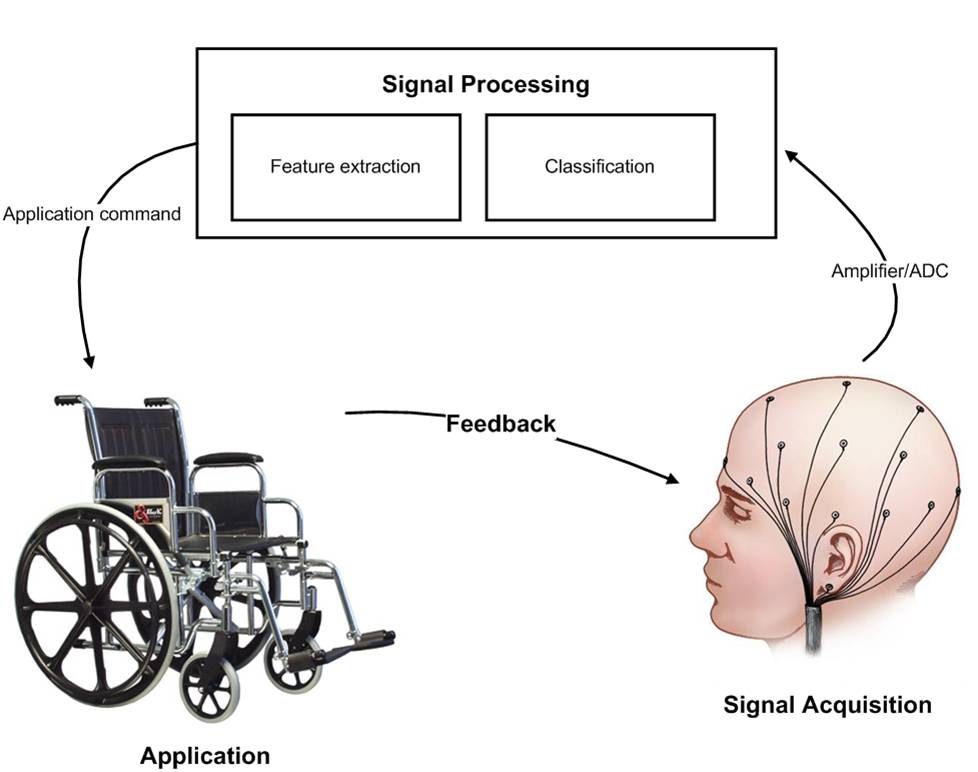
\includegraphics[width=0.5\columnwidth]{Figures/BCI-system}
\caption{A standard BCI system with signal acquisition, signal processing and application components. The system provides feedback to the user.}
\end{figure}

In this chapter, signals used in BCI are presented, along with their measurement techniques, as well as their underlying neurological phenomena.  
%--------------------------------------------------------------------------------------------------------
\section{Signal Acquisition}
\label{sec:signal_aquisition}
To measure brain activity, BCI relies on brain imaging techniques used in neurophysiology. 
The existing methods for brain imaging used in BCI can be grouped in three: electric signals, magnetic signals and hemodynamic signals.
Electric and magnetic signals are two sides of the same coin and can be grouped under the term electromagnetic signals.
%\subsection{Electromagnetic Signals}
\subsection{Local Field Potentials}
\label{neuron_electro}
The brain is made of billions\footnote{The human brain contains about 85 billion neurons~\citep{herculano-houzel_remarkable_2013}.} of interacting neurons constituting a neural network.
A neuron is made of three major parts: a cell body, an axon, and dendrites~\citep{purves_neuroscience_2008}. 
Each neuron can be connected up to thousands other neurons. 
The connection between neurons is made at a junction called \emph{synapse}. 
These junctions are often between an axon of one neuron and dendrites of the next neuron, and are referred to as axon-dendrite synaptic junctions (various other connections exist, e.g. axon-axon, dendrite-dendrite, dendrite-axon). 
The \emph{presynaptic neuron} is passing information to the \emph{postsynaptic neuron}~\citep{herculano-houzel_human_2009,purves_excitatory_2001}.

\begin{figure}[!h]
\centering
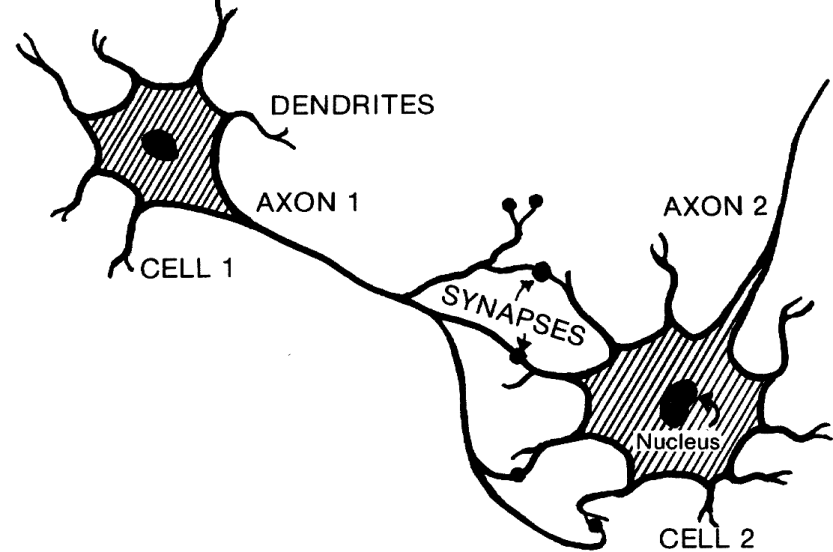
\includegraphics[width=0.5\columnwidth]{Figures/neuron-structure.png}
\caption{Neuron structure: showing main components of a neuron and its axon-dendrite synaptic connection to a neighbouring neuron \citep{purves_excitatory_2001}}
\end{figure}

%Neurons can send either an electrical signal --via \emph{electrical synapses}, or a chemical signal -- via \emph{chemical synapses}.
The information sent between two neurons is mediated by a transient modification of voltage potential called action potential or \emph{spike}.
An activated neuron fires an action potential that is sent through its synapses to its postsynaptic partners. 
The excitatory and inhibitory postsynaptic potentials (EPSPs and IPSPs) cause a flow of charged ions between point at different potentials within and outside the neurons producing an electrical current, called \emph{Local Field Potential} (LFP).
Inside the neuron, positive ions propagate from the subsynaptic area to the rest of the neuron. 
Outside the neuron, the ions that have entered the cell are replaced by an ion flow directed toward the synaptic region along the extracellular space.
%The magnetic effect of the created flow of current generates a magnetic field that propagates orthogonally to the flow of current. 

\begin{figure}[!h]
\centering
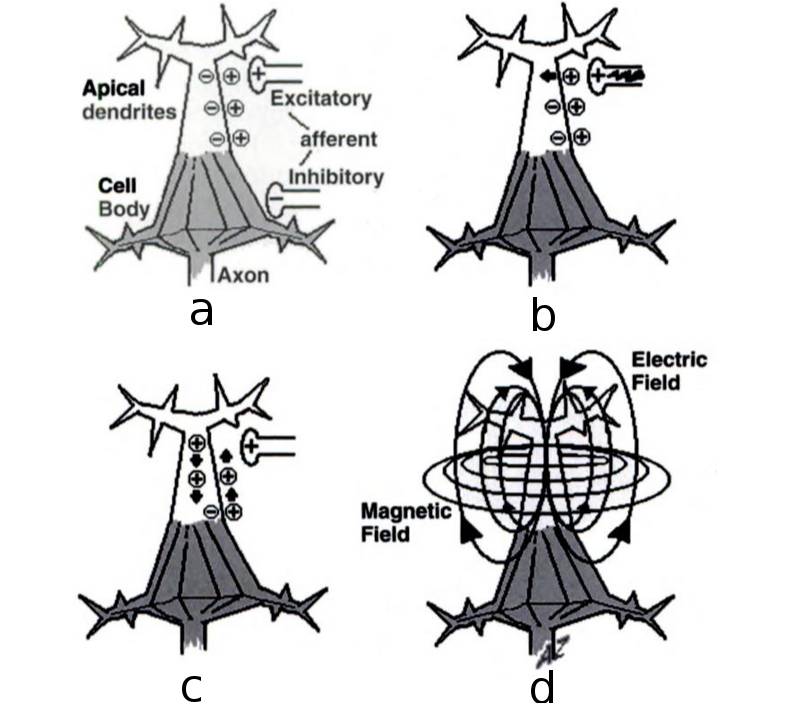
\includegraphics[width=0.5\columnwidth]{Figures/neuron-electromagnetic}
\caption{Electromagnetic activity in pyramidal neuron: (a) EPSPs converge to apical dendrites of the neuron. (b-c) Positive ions enter the neuron and propagate from synapses to the rest of the neuron. (d) the flow of current perpendicular to the apical dendrite is accompanied by a magnetic field that propagates orthogonally. \citep{proverbio_electromagnetic_2003}}
\end{figure}

\subsection{Electrical Signal Acquisition}
\label{elec_acquisition}

There are nowadays various techniques used to measure neuron electrical activities.
They can be measured on the scalp, on the cortical surface, or within the cortex.
\begin{figure}[!h]
\centering
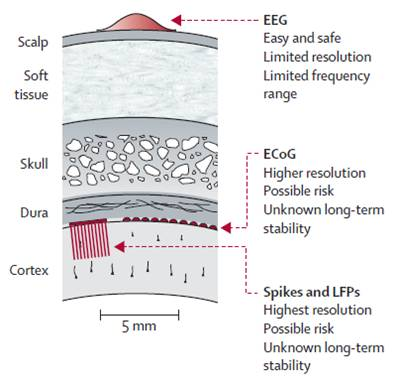
\includegraphics[width=0.5\columnwidth]{Figures/cranial-layers}
\caption{A cut through cortical layers. Electric activities can be measured from different layers. \citep[Reproduced from][]{daly_brain-computer_2008}}
\end{figure} 

\textbf{Electroencephalography} is the measurement of the brain electric activity on the scalp. 
It is the most used measurement technique in brain-computer interfaces, and is at the origin of the expansion of BCI technology. 
Electrodes are spread over the scalp to cover all regions of the cortex. 
%Few electrodes placements have been proposed with the most adopted configuration being the \emph{international 10-20 system}~\citep{niedermeyer_electroencephalography:_2005}.

%\begin{figure}[h!]
%\centering
%\subfigure[]{
%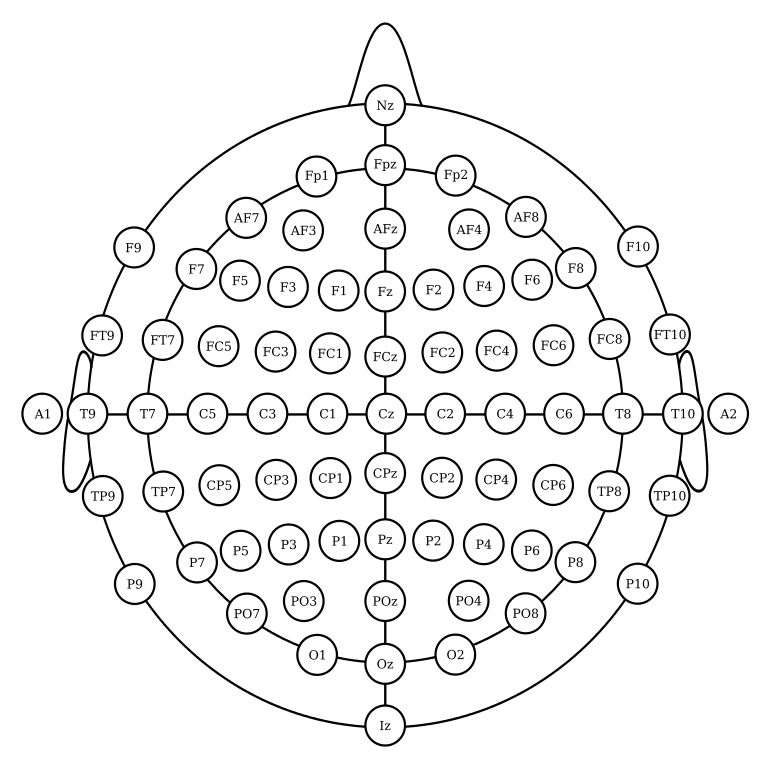
\includegraphics[width=0.5\textwidth]{Figures/eeg-electrodes-10-20}
%\label{fig:eeg-10-20}
%}
%\subfigure[]{
%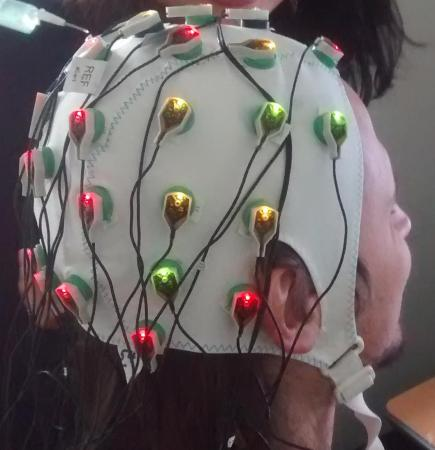
\includegraphics[width=0.45\textwidth]{Figures/eegcap}
%\label{fig:eegcap}
%}
%\caption{EEG measurement: (a) 10/20 system EEG electrodes configuration. The distance between two consecutive
%electrodes is either 10\% or 20\% of the total front-back or right-left distance of the skull. (b): Electrodes cap being fitted on a subject's head for EEG recording.} 
%\label{fig:swel_alpha}
%\end{figure} 

The changes in electrical potentials -- \emph{electroencephalogram} (EEG), recorded at an electrode are the sum of electric field of neurons that are perpendicular to the scalp beneath the electrode. 
The recorded EEG is in the order of microvolts.
EEG is recorded at an acquisition rate that can go as high as 1000 samples per second, providing a good time resolution. However, its spatial resolution is very low. It contains no depth information about the source. 
Moreover due to the dipole-like propagation of the electric potential of the source, the maximum of the distribution does not coincide with the source localisation~\citep{proverbio_electromagnetic_2003}. 
The volume conduction affects the potential field as different biological layers do not have the same electrical properties and are inhomogeneous. 
%Electricity propagate differently in different media. 
The spatial resolution of EEG is affected by this, as the measured electrical field travels through different layers of the skull.
EEG can measure brain electrical activities in spectral bands from 0 to 100 Hz. In BCI, it usually measures activities of up to 40 Hz, \textit{i.e} lower gamma band \citep{schalk_brain-computer_2011}. Activities in the upper gamma band, \textit{i.e.} from 35 Hz to 100 Hz, have been measured mostly in emotion analysis \citep{li_emotion_2009, muller_processing_1999}. 

\textbf{Electrocorticography} measures the same activity as EEG, but the electrodes that measure \emph{electrocorticogram} (ECoG) are placed directly on the exposed  surface of the cortex.  
For this reason it is also referred to as \emph{intracranial electroencephalography} (iEEG).
EcoG were recorded in humans and animals since the late 19$^{th}$ century \citep{caton_electrical_1875}.
Since then, ECoG has been used more in animals due to the fact that the placement of electrodes requires a skull surgery.
%, which is not readily doable in humans.
The study of ECoG in humans is mostly done in epileptic subjects who await surgery. 
ECoG electrodes are temporarily placed to monitor epileptic seizures and locate their focus zone~\citep{ritaccio_proceedings_2012}.
It is only very recently that ECoG has been considered for BCI~\citep{huggins_detection_1999, pfurtscheller_spatiotemporal_2003}. 
The first BCI using ECoG in humans was done by \cite{leuthardt_brain-computer_2004}.
Most BCI research is done on epilepsy patients and should coincide with the time ECoG electrodes are implanted for surgical purposes. This limit the number of ECoG-based BCI. 
There are few rare cases where ECoG electrodes have been implanted exclusively for research purposes~\citep{wang_electrocorticographic_2013, sutter_brain_1992}.

%- Electrode placement
ECoG electrodes are usually in the form of electrodes array on a grid (Figure \ref{fig:ecog}) placed above (epidural) or below (subdural) the dura mater, \textit{i.e.} the tough layer between the skull and the cortex ~\citep{schalk_brain-computer_2011}.
The location of electrodes array is determined by the clinical need in epilepsy patients~\citep{bundy_decoding_2016}. 
For patients who have the ECoG electrodes implanted exclusively for research purposes, a fMRI is done prior to the placement to determine the cortical zone of interest for the BCI task~\citep{wang_electrocorticographic_2013}.   
%- Image
%\begin{figure}[!h]
%\centering
%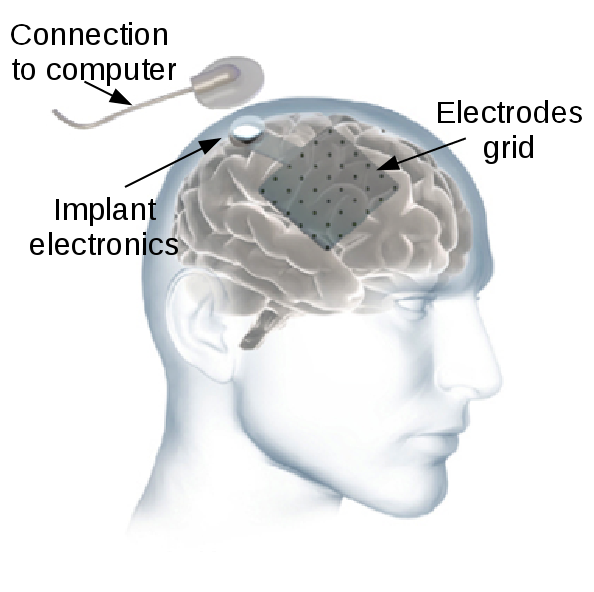
\includegraphics[width=0.3\columnwidth]{Figures/ecog-electrodes-legend}
%\caption{ECoG Electrodes. Courtesy of Ripple, Inc}
%\end{figure}

%- Acquisition frequency->time resolution - Spatial resolution - Bandwidth
ECoG is recorded at rates higher than 1 kHz, giving it a very high time resolution. 
The fact that the electrodes are placed directly on the surface of the cortex gives ECoG higher spatial resolution (\textit{i.e.} 1.25 mm for subdural recording and 1.4 mm for epidural recording~\citep{schalk_brain-computer_2011}), wider frequency bandwidth (0 to 500 Hz), and higher amplitude (\textit{i.e.} 50 to 100 $\mu V$) than EEG~\citep{schalk_brain-computer_2011, leuthardt_brain-computer_2004, spuler_decoding_2014}.
With a wider bandwidth, ECoG can capture neural electrical activity in the $\gamma$-band -- which ranges from 30 Hz up, with higher precision than EEG. 
ECoG BCI research has shown that activity in the $\gamma$-band provide deeper information about movement and movement imagery such as direction and velocity both 2-dimensional and 3-dimensional \citep{bundy_decoding_2016, leuthardt_brain-computer_2004}.

\begin{figure}[h!]
\centering
\subfigure[]{
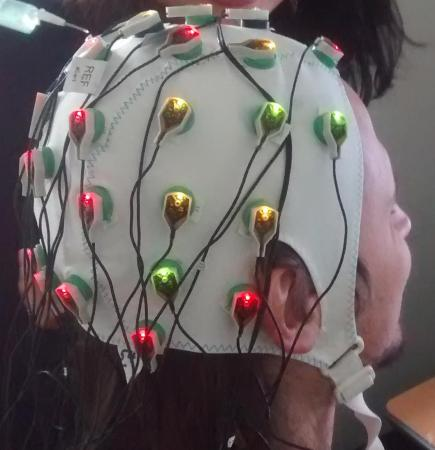
\includegraphics[width=0.3\textwidth]{Figures/eegcap}
\label{fig:eegcap}
}
\subfigure[]{
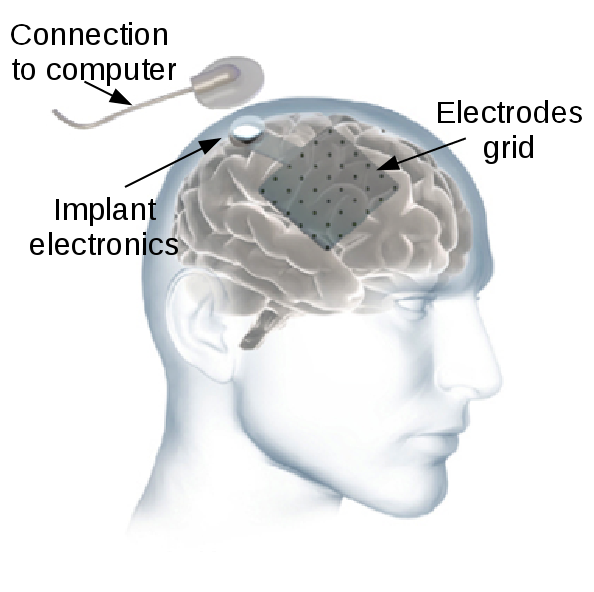
\includegraphics[width=0.3\textwidth]{Figures/ecog-electrodes-legend}
\label{fig:ecog}
}
\subfigure[]{
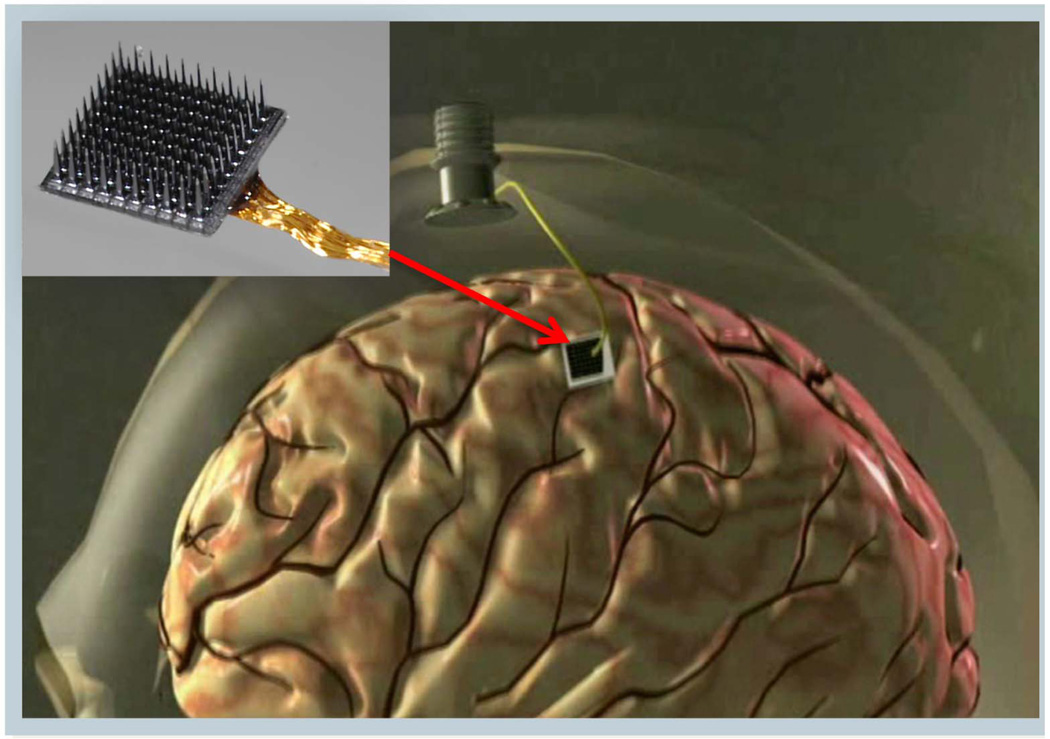
\includegraphics[width=0.3\textwidth]{Figures/intracranial-electrodes}
\label{fig:intracranial}
}
\caption{electric signals electrodes: (a) EEG electrodes cap being fitted on a subject's head for recording. (b) ECoG Electrodes. Courtesy of Ripple, Inc. (c) A silicon-based cortical MEA (inset); implanted for intracortical neural recording via a percutaneous connection to a skull mounted pedestal connector \citep{homer_implants_2013}.} 
\label{fig:electrodes-electric}
\end{figure} 

    
\textbf{Spikes} and \textbf{Local Field Potentials} are intracortical measures of neural activities. 
The purpose is to measure the activity of a single neuron via its spikes, or the sum of activities of a small population of neurons local to a region -- the local field potentials.
Recording of neuronal spikes done approximately 50 years ago has shown that movement intent modulates spike timing from neurons of the motor cortex. 
%\begin{figure}[!h]
%\centering
%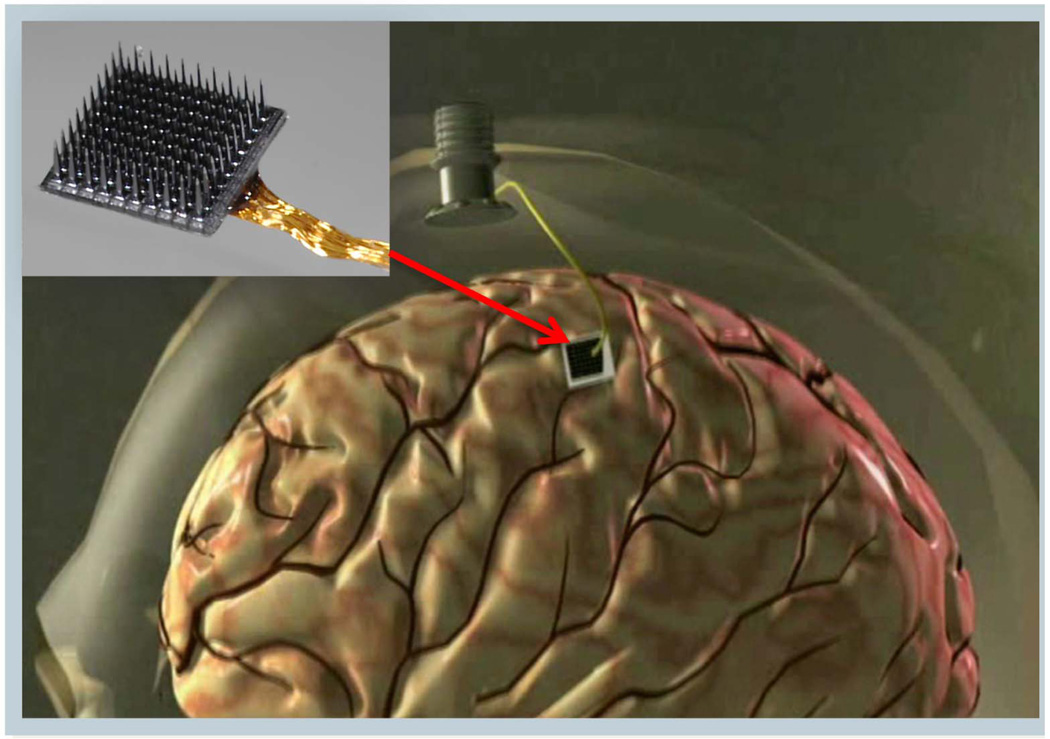
\includegraphics[width=0.5\columnwidth]{Figures/intracranial-electrodes}
%\caption{A silicon-based cortical MEA (inset); implanted for intracortical neural recording via a percutaneous connection to a skull mounted pedestal connector \citep{homer_implants_2013}.}
%\end{figure}

The first clinical application using intracortical recording -- also called stereoelectroencephalography,  was achieved in 1998~\citep{kennedy_restoration_1998}.
The electrodes are placed in the motor cortex. 
A fMRI or MRI is performed before the implant to locate the precise location.
From the year 2000, substantial research has been done on these recording techniques, mostly on non-human primates~\citep{serruya_brain-machine_2002, taylor_direct_2002, musallam_cognitive_2004, santhanam_high-performance_2006, golub_motor_2014}. 
It has shown that it is possible to control devices such as prosthetics and achieve complex tasks such as 3D control, and reaching and grasping action with prosthetic devices by using motor cortex spiking pattern~\citep{homer_implants_2013}.
%Studies done on monkeys have paved the way to intracortical BCI for humans. 
In humans, intracortical BCI has been studied on patients with spinal cord injuries~\citep{hochberg_neuronal_2006,hochberg_reach_2012}, amyotrophic lateral sclerosis~\citep{kennedy_restoration_1998}, brainstem stroke~\citep{kennedy_direct_2000}, and mitochondrial myopathy~\citep{kennedy_computer_2004}.
By recording activities of individual neurons, recorded signals are not affected by activities happening in different brain regions. With electrodes implanted in different regions of the cortex, intracortical BCI could take parallel commands and offer many degrees of freedom. 
      
\subsection{Magnetic Signal Acquisition}
\label{magnet_aquisition}
Electric and magnetic signals are two side of the same coin. 
They are both created by the same synaptic exchange between neurons~\ref{neuron_electro}.
The magnetic effect of electric currents in neurons generates a magnetic field that propagates orthogonally to the flow of current~\citep{gazzaniga_cognitive_2013, proverbio_electromagnetic_2003}. 

\textbf{Magnetoencephalography} (MEG) is the measure of neurons magnetic field on the scalp. 
It is a neuroimaging technique used in neuroscience and clinical applications. 
It is very related to EEG as both are measured on the scalp. 
Both magnetic and electric fields propagate through different cranial layers before being measured on the scalp.
Nonetheless MEG has an advantage over EEG; the magnetic field is not as influenced by the medium as is the electrical field. 
A drawback in measuring the magnetic activity of brain is that it is 
8 orders of magnitude bellow 
%100 millionth the size of 
the earth's magnetic field (in the order of $10^{-15}$ Tesla). 
Due to this, it cannot be measured in ``open air".
Electromagnetic isolation chambers are needed, making the MEG acquisition equipment bulky and expensive. 
MEG sensors are usually made of a magnetometer and two orthogonal planar gradiometers. 
Ranging from 64 to more than 300, MEG sensors are immersed in liquid helium and attached on a concave bottom of a container, where they typically lie at a distance of  3 - 4 cm from the cortex. 
The weak extracranial magnetic fields are amplified and transformed into a voltage \citep{paetau_magnetoencephalography_2002}.



\begin{figure}[h!]
\centering
\subfigure[]{
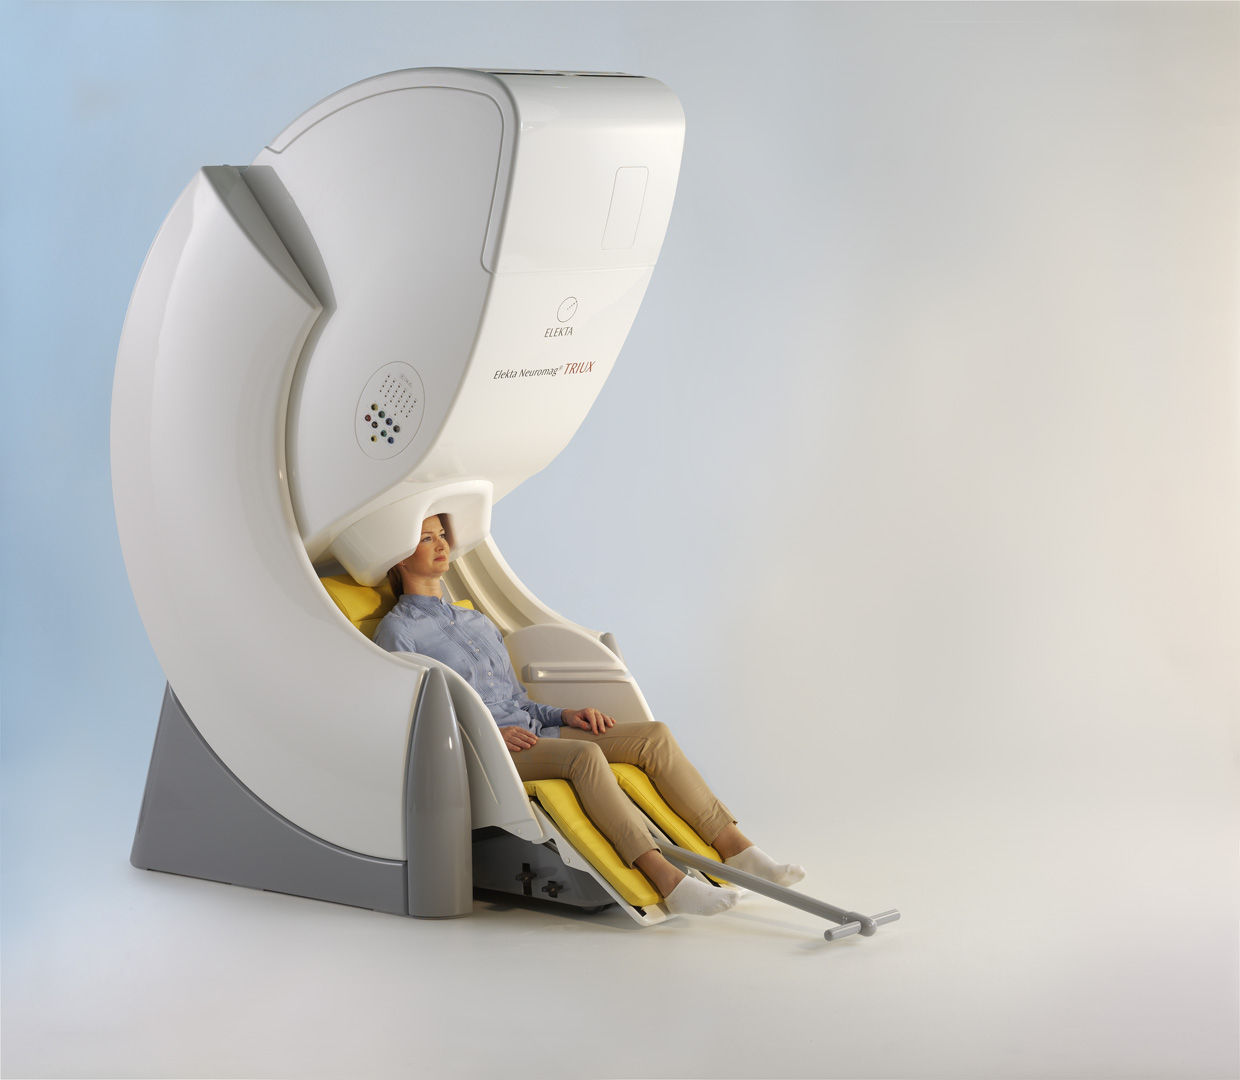
\includegraphics[width=0.45\textwidth]{Figures/MEG_scanner_elekta}
\label{fig:meg-sys-chamber}
}
\subfigure[]{
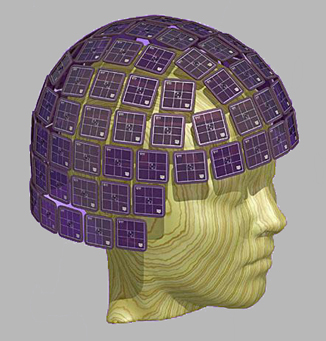
\includegraphics[width=0.45\textwidth]{Figures/MEG_sensors}
\label{fig:meg-sys-sensors}
}
\caption{Elekta MEG acquisition system. (a) A MEG shield chamber for electromagnetic isolation  (b) MEG sensors configuration. Each sensor location is equipped with three sensors: a magnetometer  that measures normal field component, and two orthogonal planar gradiometers that measure gradient components~\citep{team_elekta_2016}.}
\label{fig:meg-system}
\end{figure} 

MEG has similar temporal resolution to EEG, but has a higher spatial, and can better capture modulations in brain signals, thus improving control and information transfer rates in BCI. 
EEG and MEG can also be co-recorded in BCI tasks and used in to improve BCI performances \citep{mellinger_meg-based_2007, henson_parametric_2011, foldes_meg-based_2015}.

\subsection{Hemodynamic Techniques}
\label{optical_sig}

While EEG, ECoG, LFP, spikes, and MEG measure the direct electromagnetic activities of neurons, there are other neuroimaging techniques that measure the metabolic effect of neurons electrical activities.
In fact there is a relationship, \textit{i.e.} \emph{neurovascular coupling}, between neuronal activity and subsequent regional blood volume and flow.
This coupling is explained by the fact that firing neurons involved in a neurological task requires more energy and oxygen, resulting in an increase of blood flow and oxygenation. 
The active neurons in the region do not use the totality of the provided oxygen. 
This results in a change in the ratio between oxygenated (oxyHb) and deoxygenated (deoxyHb) hemoglobin. 
This metabolic response to neuron activities is called the \emph{hemodynamic response} and can be measured using different techniques such as Magnetic Resonance Imaging (MRI), Functional Magnetic Resonance Imaging (fMRI), Positron Emission Tomography (PET), Near Infrared Spectroscopy (NIRS), and Functional Near Infrared Spectroscopy (fNIRS).
fMRI, NIRS, and fNIRS have a possibility of real time recording required for brain-computer interfaces.

\textbf{fMRI} or Blood-oxygen-level-dependent (BOLD) fMRI uses magnetic resonance to measure the concentration of oxyHb and deoxyHb making use of the difference in their magnetic properties \citep{matthews_functional_2004, gosseries_[functional_2008, huettel_functional_2004, sitaram_fmri_2008}.
fMRI consist of multiple scans of MRI to capture brain activity. 
A transmitter coil covering the head is needed to generate a magnetic field responsible for the resonance and relaxation in oxyHb and deocyHb. 
fMRI have high spatial resolution (i.e few millimetres) and low temporal resolution (\textit{i.e.} few seconds) compared to electromagnetic brain signals.
fMRI-BCI capitalises on the ability of fMRI to locate brain activity to the millimetre, to characterise different spatial distribution of brain functions as BCI commands \citep{sitaram_fmri_2007, yoo_braincomputer_2004}. 
Though fMRI-BCI can achieve high classification accuracy, they are held back by the low temporal resolution that limit the speed of MRI scans and the information transfer rate of the interface.
Furthermore, the size and setup of fMRI acquisition equipment limit the mobility of users.

\textbf{NIRS} and \textbf{fNIRS} are recent hemodynamic techniques introduced in the late 1980s. 
They measure the intensity of light propagated through brain tissues. Since the concentrations of oxyHb and deoxyHb in brain tissues are indicators of neural activity, f/NIRS use the relationship between transmitted light and the concentration of the medium (i.e chromophores such as oxyHb and deoxyHb) to calculate these concentrations by shining near-infrared light on the head and measuring the intensity of the exiting light as shown in Figure \ref{fig:nirs}.

\begin{figure}[h!]
\centering
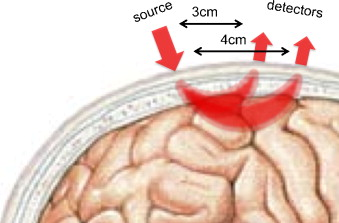
\includegraphics[width=0.45\textwidth]{Figures/nirs}
\caption{Trajectory of near-infrared light in the human brain. \citep[Reproduced from][]{gervain_near-infrared_2011}.}
\label{fig:nirs}
\end{figure} 

f/NIRS has a good spatial resolution (few millimetres), better compared to electromagnetic signals measured on the scalp (\textit{i.e.} EEG and MEG), but lower than fMRI.
The acquisition equipment is lighter, easy to use, and enhances mobility of the subject. 
NIRS is tolerant to movement whereas other signals' recording techniques either does not allow user movement (e.g. fMRI, MEG) or the signal quality is distorted by movement (e.g. EEG).
As with fMRI-BCI, f/NIRS-BCI also relies on the ability to separate brain function based on their spatial distribution. 
%Though it spatial is lower compared to fMRI, f/NIRS-BCIs are easier to use. 
Although the spatial resolution of f/NIRS is lower than the resolution of fMRI, f/NIRS-BCIs are easier to use than fMRI-BCIs.
They have good classification accuracy, but are still slower than BCI that use electromagnetic signals. 
The BCI tasks are also limited to brain functions that can be measured close to the scalp. 
In fact f/NIRS cannot measure deep brain activity, because of light penetration which is limited to 15 mm and 5~mm into the cortex, for infants and adults respectively. 

%that has the merit of enhancing the mobility of the subject. While in EE 

%*The fact that it is also an indirect measurment of neuronal activity give it a low temporal resolution similar to fMRI.(sampling freq <= 10) but is faster than fMRI (0.5Hz)

\subsection{Discussion}
\label{subsec:signal_acq_discussion}

Several neuroimaging techniques have the potential of being used in BCI. 
Each has characteristics that can be used to successfully classify brain functions.
One requirement that all should meet to be considered as an input signal in BCI applications is the ability of near real time recording/scanning. 
%They also have limitations that will limit their efficacy in BCI. 
%A trade-off should be decided on to choose an optimal signal for BCI.

Neuroimaging techniques such as fMRI and MEG limit the mobility of the user and limit  brain-computer interface to few applications. 
Moreover fMRI is not real time.
Despite their good spatial resolution and temporal resolution (for MEG), they are not adapted for daily life interaction. 
f/NIRS is a good trade-off between user mobility and spatial resolution of the acquired signal. 
However, the fact that, as fMRI, it relies on hemodynamic response implies a low temporal resolution that might not be enough to capture transient brain responses to stimuli used in BCI, and exposes it to physiological noise such as cardiac cycle and respiratory effect that alter blood oxygenation more than other measurement techniques. 
In terms of user mobility and ability to capture fast brain response, electrical signals (EEG, ECoG and intracortical signals) remain so far the best options.
It is proven that intracortical BCIs offer high interaction performances by decoding complex brain activities. 
However the risk and uncertainties surrounding the intracortical implantation of electrodes are still an issue for its recognition by the public. It is judged to be too invasive.
The intracranial version of EEG -- ECoG, alleviates many problems of EEG-based BCI, namely its vulnerability to noise (\textit{i.e.} ocular, muscular and environmental). 
Although it is less invasive compared to intracortical measurement, ECoG still requires surgery for electrodes placement. 

Despite its relatively low spatial resolution and vulnerability to noise, EEG remains the sole technique that offers fast tracking of neural activities, affordable and light recording equipment allowing BCI users' mobility, safety and ease of use.
It is vastly adopted as the input signal for BCI. 
However, some researchers believe that the future of BCI lies in invasive techniques. 
They argue that non-invasive techniques can only represent a limited number of brain responses -- thus limited degrees of freedom, and that EEG weaknesses are hardly overcome. 
Another argument is that, for the same neurological phenomenon, non-invasive BCI requires longer training periods for the users  to learn to produce a particular brain response voluntarily, and despite the training non-invasive BCI still have high error rates. %~\citep{birbaumer_brain-computer-interface_2006}. 
A further argument is that although non-invasive medically, EEG measurement technique can also be seen as invasive in terms of human machine interaction: the gel, the tight electrode cap, the restriction to blink eyes during recording, etc. might be seen as invasive.
These arguments have not stopped the EEG-based BCI community from pushing the limits. 
Wolpaw and McFarland disapproved the argument against non-invasive BCI by showing that with a comprehensive user training and good learning algorithms, EEG-based BCI could provide multidimensional point-to-point movement control that falls within the range of invasive BCI performances~\citep{wolpaw_control_2004}.
Research on improving EEG-based BCI performance has increased all the more, with better tools for the processing of EEG signals \citep{gramfort_mne_2014}, and encouraging results \citep{mattout_improving_2013, kalunga_online_2016}.  

In conclusion, while other neuroimaging might be adequate for some BCI applications (e.g. neurofeedback), EEG constitutes a reasonable choice for signal input in BCIs for assistive purposes (e.g. communication and mobility). 
EEG-based BCIs are well tolerated with their limitations by patients with the need to communicate without their muscular systems~\citep{kubler_severity_2005, grubler_psychosocial_2014}. 
With effort from different fields involved in BCI research, it is possible to reach better performance and tend toward those reported with invasive BCIs.  

  
%\subsubsection{Signal Processing}
%- Explain the steps that are taken and examples of each
%\subsubsection{Application interface} %Mention Feedback
%- Name applications of BCI and examples, and how feedback is provided
%
%Brain computer interfaces decipher brain signal characteristics related to subject intention or reaction to a stimulus into tengible action. 

%\subsection{Brain Computer Interface Categorisation}
%\label{subsec:bci_tech_category}
%\subsection{Neurological Phenomena}
%\label{subsec:bci_tech_neuro_phenomena}
%
%\subsection{Brain Computer Interface Performance Evaluation}
%\label{subsec:bci_tech_performance_evaluation}
%
%\subsection{Brain Computer Interface state-of-the art} %Mention successful examples of BCI and present their performance
%\label{subsec:bci_tech_sate}
\section{Neurological Phenomena}
\label{sec:lit_survey_neuro_phenomena}

In deciphering brain signals, brain-computer interfaces identify a specific feature -- a \emph{neurological phenomenon}, from the signal that is associated with a given user's intention. 
Neurological phenomena are variations in the brain signals associated with a cognitive activity (\textit{i.e.} cognitive conscious information processing),  or in response to a physical stimulus.
Neurological phenomena induced by cognitive activities are said to be \emph{endogenous}, while those triggered by external physical stimulus are said to be \emph{exogenous}.
Respectively, BCIs that rely on exogenous neurological phenomena are classified as exogenous or dependent BCIs as they dependent on an external stimulus, and their counterparts that rely on endogenous phenomena are classified as endogenous or independent BCIs as  no external stimulus is needed.
BCI research has mainly focused on the following phenomena: Event Related Desynchronisation (ERD) and Event Related Synchronisation (ERS), Event Related Potential (ERP), and visually Evoked Potential (VEP). 
There are discussed in the details in the next lines.
%####################################################################################################################################
\subsection{Event-Related Synchronisation-based BCI}
\label{subsec:ERD/S-BCI}

\subsubsection{Event-Related Desynchronisation and Synchronisation}

%Several kinds of events -- sensory or motor -- induce events-related
%potentials in the brain signals. 
%
%Manifested as deflections in the brain
%signal's voltage, event-related potentials are believed to be a result of a reorganisation of the phases or changes in specific frequency bands in the ongoing brain signals \cite{pfurtscheller1999ERDreview}. 
Event related (de)synchronisation are either a decrease --\emph{event-related desynchronisation} (ERD), or an increase -- \emph{event-related synchronisation} (ERS), of power in a given frequency band during a cognitive activity\citep{pfurtscheller_graphical_1977, pfurtscheller_event-related_1977, pfurtscheller_event-related_1994}; they are endogenous phenomena. 
%The former is called event-related desynchronisation or ERD and the latter event-related synchronisation or ERS \cite{Pfurtscheller1977Graph} \cite{Pfurtscheller1992} \cite{Pfurtscheller1977Event}.

\par \cite{pfurtscheller_event-related_1999} interpret ERD as an electrophysiological correlate of activated cortical areas involved in processing of sensory or cognitive information or production of motor behaviour. 
ERD/ERS is mainly observed in the 
$\alpha$ rhythm, the $\mu$ rhythm also referred to as the upper $\alpha$ rhythm, the $\beta$ rhythm and the $\gamma$ rhythm.
The $\alpha$ rhythm ranges from 8 to 12~Hz, the $\mu$ between 10 and 12~Hz, the $\beta$ rhythm between 12~ and 30~Hz, 
and the $\gamma$ rhythm between 30 and 60~Hz.
The low frequencies of oscillations in the brain signal are caused by synchronous neural activities that involve a large number of neurons. 
Hence slow oscillations are measurable in a large area of the brain. 
On the other side, assemblies of only small numbers of neurons in synchrony  oscillate at high frequencies \citep{singer_synchronization_1993}.  
The amplitudes of oscillations being proportional to the number of synchronous neurons, low frequencies have higher amplitude and high frequencies smaller ones. Therefore ERD/ERS in $\alpha$-rhythm are more visible than in any other
frequency bands.% (ie. high amplitude and wide topographical distribution). This is illustrated in Figure~\ref{fig:alphawave}.

%\begin{figure*}[!ht]
%    \centering
%    \includegraphics[width=4.0in]{Figures/alphawave.pdf}
%    \caption{\footnotesize{EEG recorded on 8 channels in the occipital region. The signal
%    is band filtered from 8 to 60Hz. The amplitude (y-axis) is in $\mu$-volts
%    and the time (x-axis) in seconds. The subject is relaxed with closed eyes.
%    A synchronisation in the alpha wave of approximately 10Hz is visible on
%    all channels with high amplitude.}}
%    \label{fig:alphawave}
%\end{figure*}

Though easily measurable, lower $\alpha$ wave ERDs cannot be used to discriminate between tasks due to their wide topographical distribution. 
Moreover they might be obtained in response to any task. % \cite{pfurtscheller1999ERDreview}. 
$\mu$ rhythm ERDs, however, are topographically restricted to some brain areas and happen only in response to specific activities. $\mu$-rhythm ERD provoked by a given task will be observed mainly in the brain cortex in charge of the task. 
This specificity to tasks offers a possibility of discrimination amongst them~ \citep{pfurtscheller_event-related_1999}.
%This offers a possibility for discrimination between tasks. 

\subsubsection{Motor Imagery BCI Systems}

The cognitive tasks used in current ERD/ERS-based BCI systems include motor imagery \citep{pfurtscheller_motor_2001}, mental tasks, e.g. sitting idle, doing a multiplication, composing a song \citep{kumar_design_2010}, composing letters, counting, rotating objects \citep{faradji_brain-computer_2009}), or a combination of mental tasks and motor imagery tasks \citep{penny_eeg-based_2000, ozmen_discrimination_2011}.% \cite{Penny2000EEG-based,Ozmen2011Discrim}. 

A user performs a cognitive task while his brain signals are being recorded, for further processing and classification.
The majority of studies conducted in ERD/ERS-based BCI are carried out on synchronous systems. 
Figure~\ref{fig:ERDSparadigm} illustrates a synchronous ERD/ERS-based BCI paradigm. 
The mental task is performed from the cue onset for a specific period of time. The trial starts with a beep. The user looks at the screen -- where a fixation cross is displayed -- waiting for the cue that will indicate the mental task to be performed. 
\begin{figure*}[!ht]
    \centering
    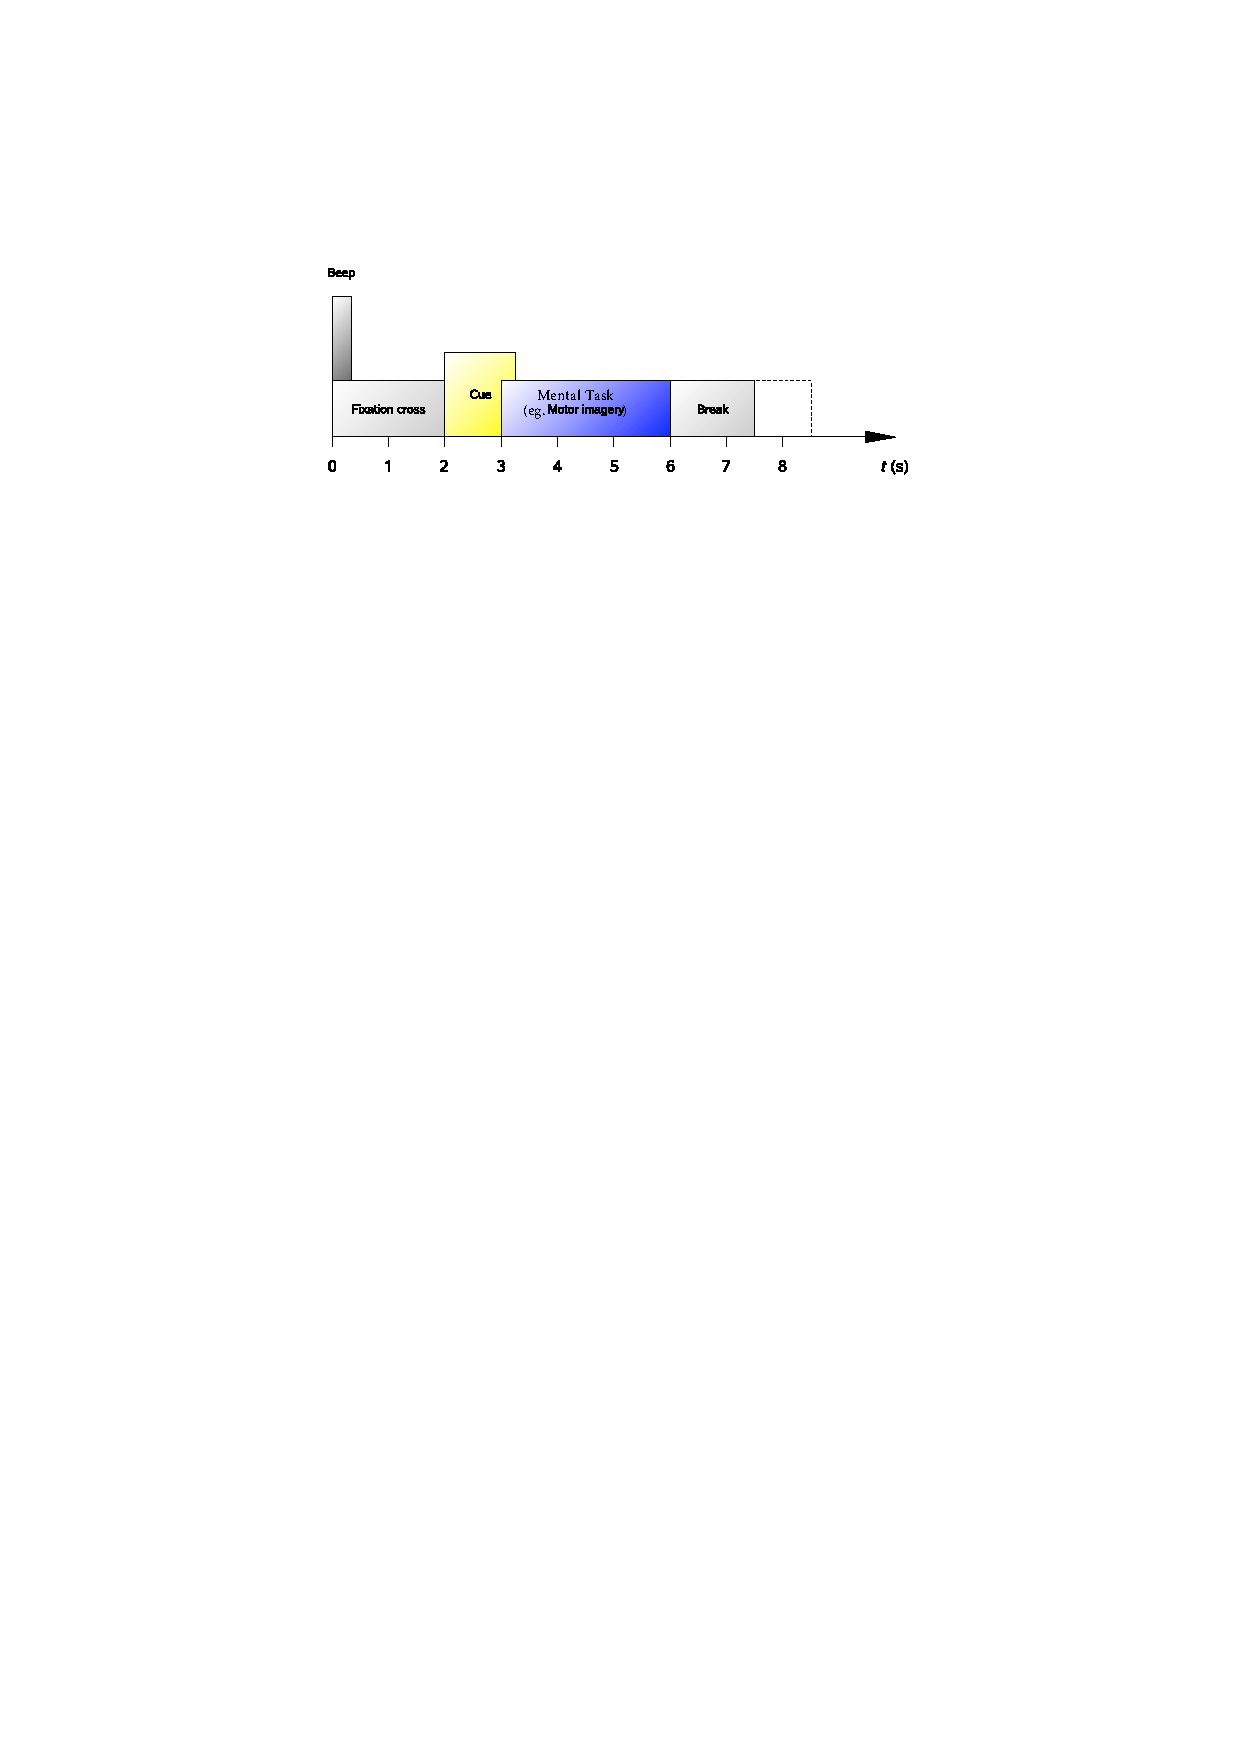
\includegraphics[width=0.5\columnwidth]{Figures/ERDS-paradigm.pdf}
    \caption{\footnotesize{Standard ERD/ERS-based BCI system paradigm. The
    break before the next trial should last at least a second to allow the changes in the
    ongoing EEG/MEG to recover. }}
    \label{fig:ERDSparadigm}
\end{figure*}
\par

Motor imagery provides the most intuitive and affordable cognitive task for the large population of users and has therefore dominated BCI research. It also has a record of best classification accuracy. 
The tasks that induces the most separable features in the EEG are the imagery of right-hand movement, the imagery of left-hand movement, the imagery of foot movement and the imagery of tongue movement~\citep{ang_filter_2012}. 
When a person is at rest (\textit{i.e.} not involved any motor activity), there is a high  activity in the 8-12 Hz band (\textit{i.e.} $\mu$ rhythm) and the 18-26 Hz band (\textit{i.e.} $\beta$ rhythm) in the motor cortex. This activity is also known as \emph{sensory motor rhythm} (SMR).
It has been shown that for right hand movement there is a decrease, ERD, of SMR in the left hemisphere of
the sensory-motor cortex, and the ERD occurs prior to the actual movement, during the preparation phase preceding the movement \citep{pfurtscheller_event-related_1999}. 
It has also been established that motor imagery (mental imagination of movements) activates similar brain areas (functions) to those activated during the preparation phase of actual movement \citep{jeannerod_mental_1995, roland_supplementary_1980}.
In general, voluntary hand movement results in bilateral ERD in the hand area and ERS in the foot area (see homunculus in~\ref{fig:homunculus}); while a simple mental imagination of the same movement results  in the contralateral  $\beta$ ERD and ipsilateral $\beta$ ERS, both in the hand area \citep{pfurtscheller_existence_1997, pfurtscheller_event-related_1994, toro_c._and_deuschl_g_and_thatcher_r_and_sato_s._and_kufta_c_and_hallett_m._event-related_1994}.
The fact that in mental imagination of one-sided hand movements the ERD remains mostly limited to the contralateral hemisphere is of key value in the classification of motor imagery-based BCI. 
%Left and right hand imagery can be differentiated on the grounds of their asymmetrical electrocortical responses.
%Only these tasks provide a possibility of topographical discrimination between their respective elicited
%ERD/ERS in the $\mu$ and $\beta$ rhythm. 
Several studies \citep{lotte_review_2007} have focused on the imagery of right hand and left hand movement -- since these two tasks present the most discriminative characteristics because of their asymmetrical electrocortical responses -- to build a 2-class BCI and have the best classification accuracy achieved in ERD/ERS-based BCI \citep{zhang_bci_2012}. 
It is to be mentioned that ERD elicited by motor imagery of different parts of an upper limb cannot be discriminated \citep{pfurtscheller_event-related_1999}. 
For instance, the imagery of left wrist movement and any left finger movement will activate the same brain region (contralateral ERD and ipsilateral ERS in the hand region) as the one activated during the imagery of the left hand. 
For lower limbs, imagination of either foot movement results in a $\mu$ or $\beta$ ERD in the foot area between both hemispheres such that it becomes impossible to discriminate between imagery of the left foot and of the right foot \citep{pfurtscheller_event-related_1999}. It is expected that the imagery of foot movement activates the foot area and the imagery of the tongue, the tongue area. 
%However it is generally observed that these tasks result in ERD across unexpected brain areas, making the classification task more difficult. 
However it is generally observed that the area activated by these two tasks are mixed up and not easily interpretable. 

BCI systems must therefore use some complex algorithms to extract the most discriminative features and achieve a multiclass discrimination, e.g. 4-class: right hand, left hand, feet, and tongue~\citep{dornhege_boosting_2004, brunner_spatial_2007}.

\begin{figure*}[!ht]
    \centering
    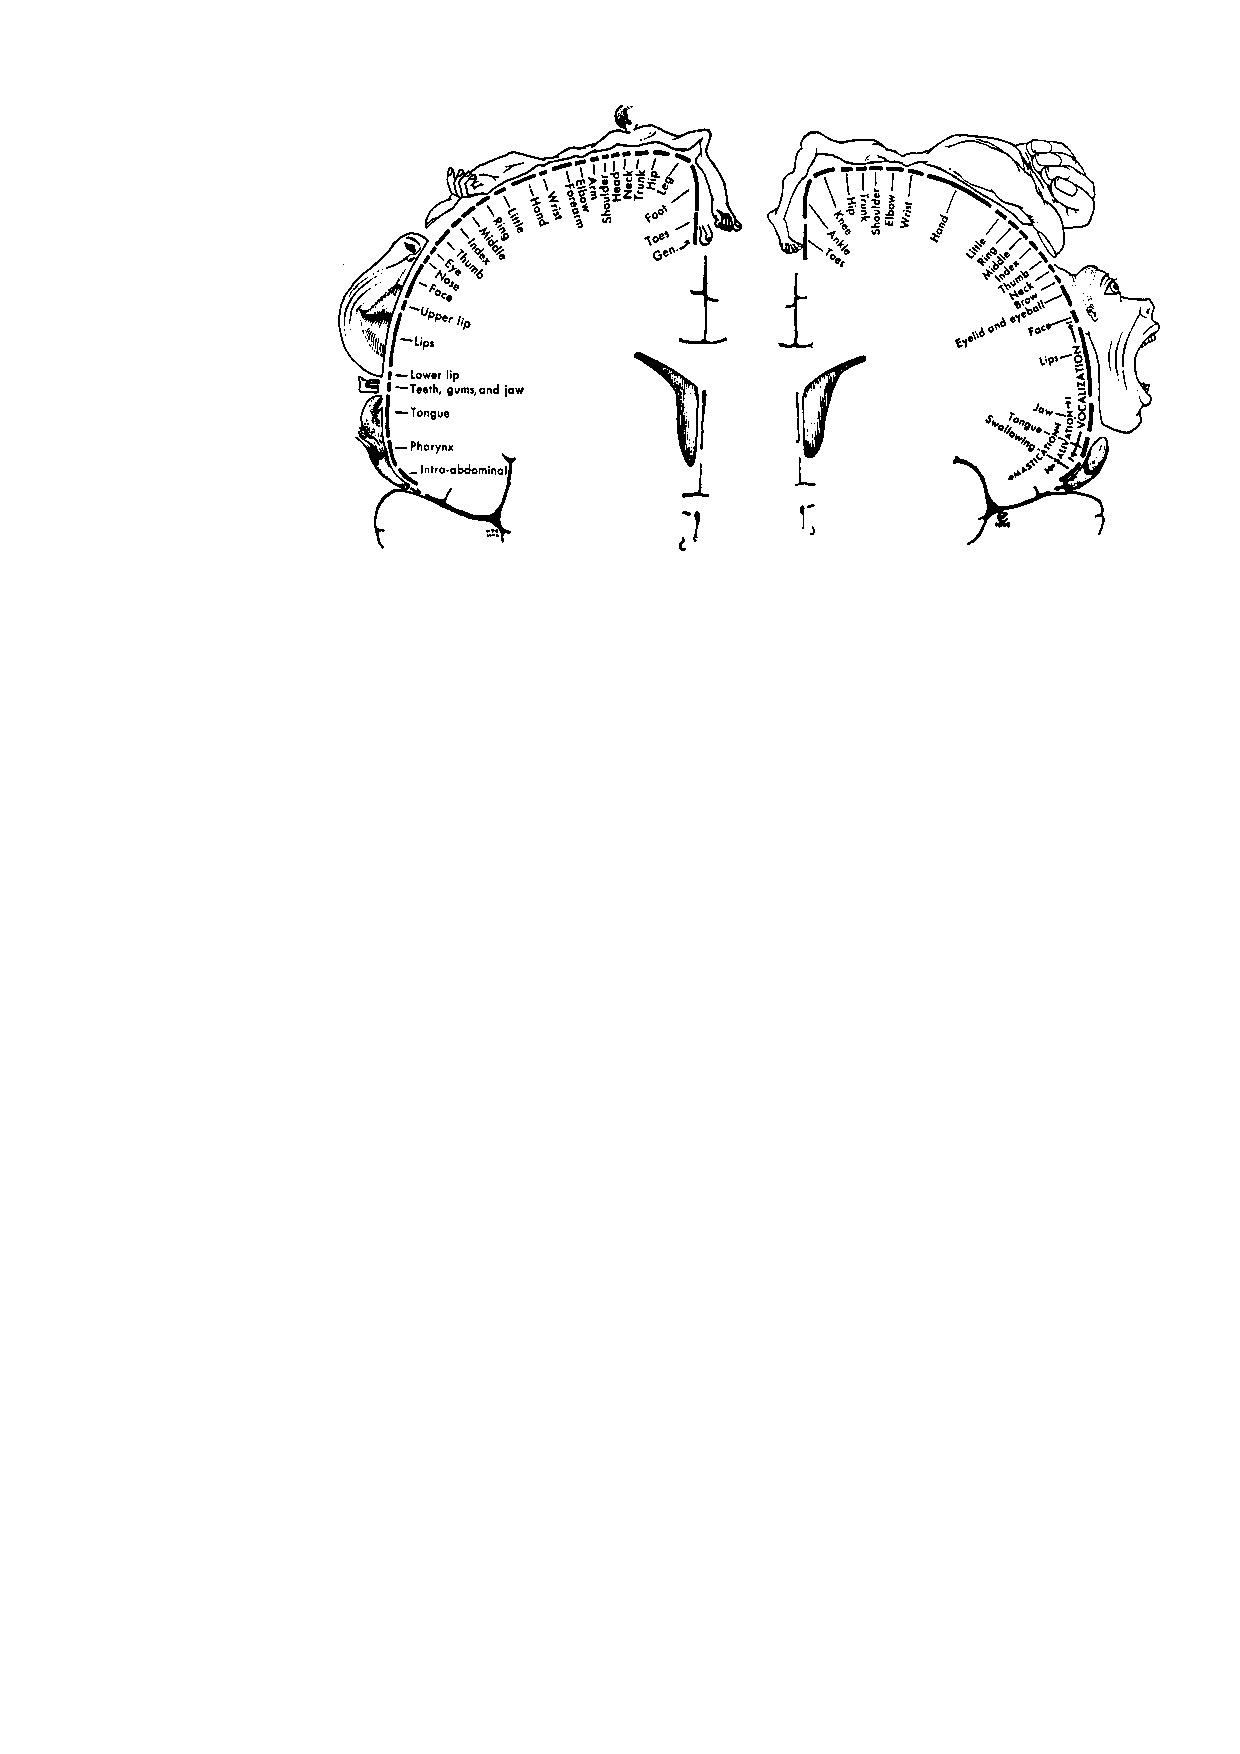
\includegraphics[width=4.0in]{Figures/homunculus.pdf}
    \caption{Sensory homunculus on the left and Motor homunculus on the right.
    The cortical homunculus initially developed by Dr. Wilder Penfield
    shows a disproportionate human body laid on the cortex from the prefrontal
    cortex(top) to the cerebellum (bottom). The size of a given body part
    of the homunculus is descriptive of the amount of cerebral tissue or cortex
    devoted to the specific body region which is proportional to how richly
    innervated that region is.
    This image is taken from \citep{schoot_penfields_1993} }
    \label{fig:homunculus}
\end{figure*}


%\note{something on other mental tasks? see references at the begining of section}
%The majority of studies conducted in ERD/ERS based BCI are carried out on
%synchronous systems. Figure~\ref{fig:ERDSparadigm} illustrates a synchronous
%ERD/ERS based BCI paradigm. The mental task is performed from the cue onset
%for a specific period of time. The trial starts with a beep. The user looks
%at the screen -- where a fixation cross is displayed -- waiting for the cue
%that will indicate the mental task to be performed. New approaches are being
%developed for the implementation of asynchronous ERD/ERS based BCI
%\cite{Satti2009,Lotte2008,Galan2008} where the BCI system continuously
%classifies the ongoing brain activities, not only into a specific class
%corresponding to the performed mental task, and differentiates between IC and
%NC states.
%
%\begin{figure*}[!ht]
%    \centering
%    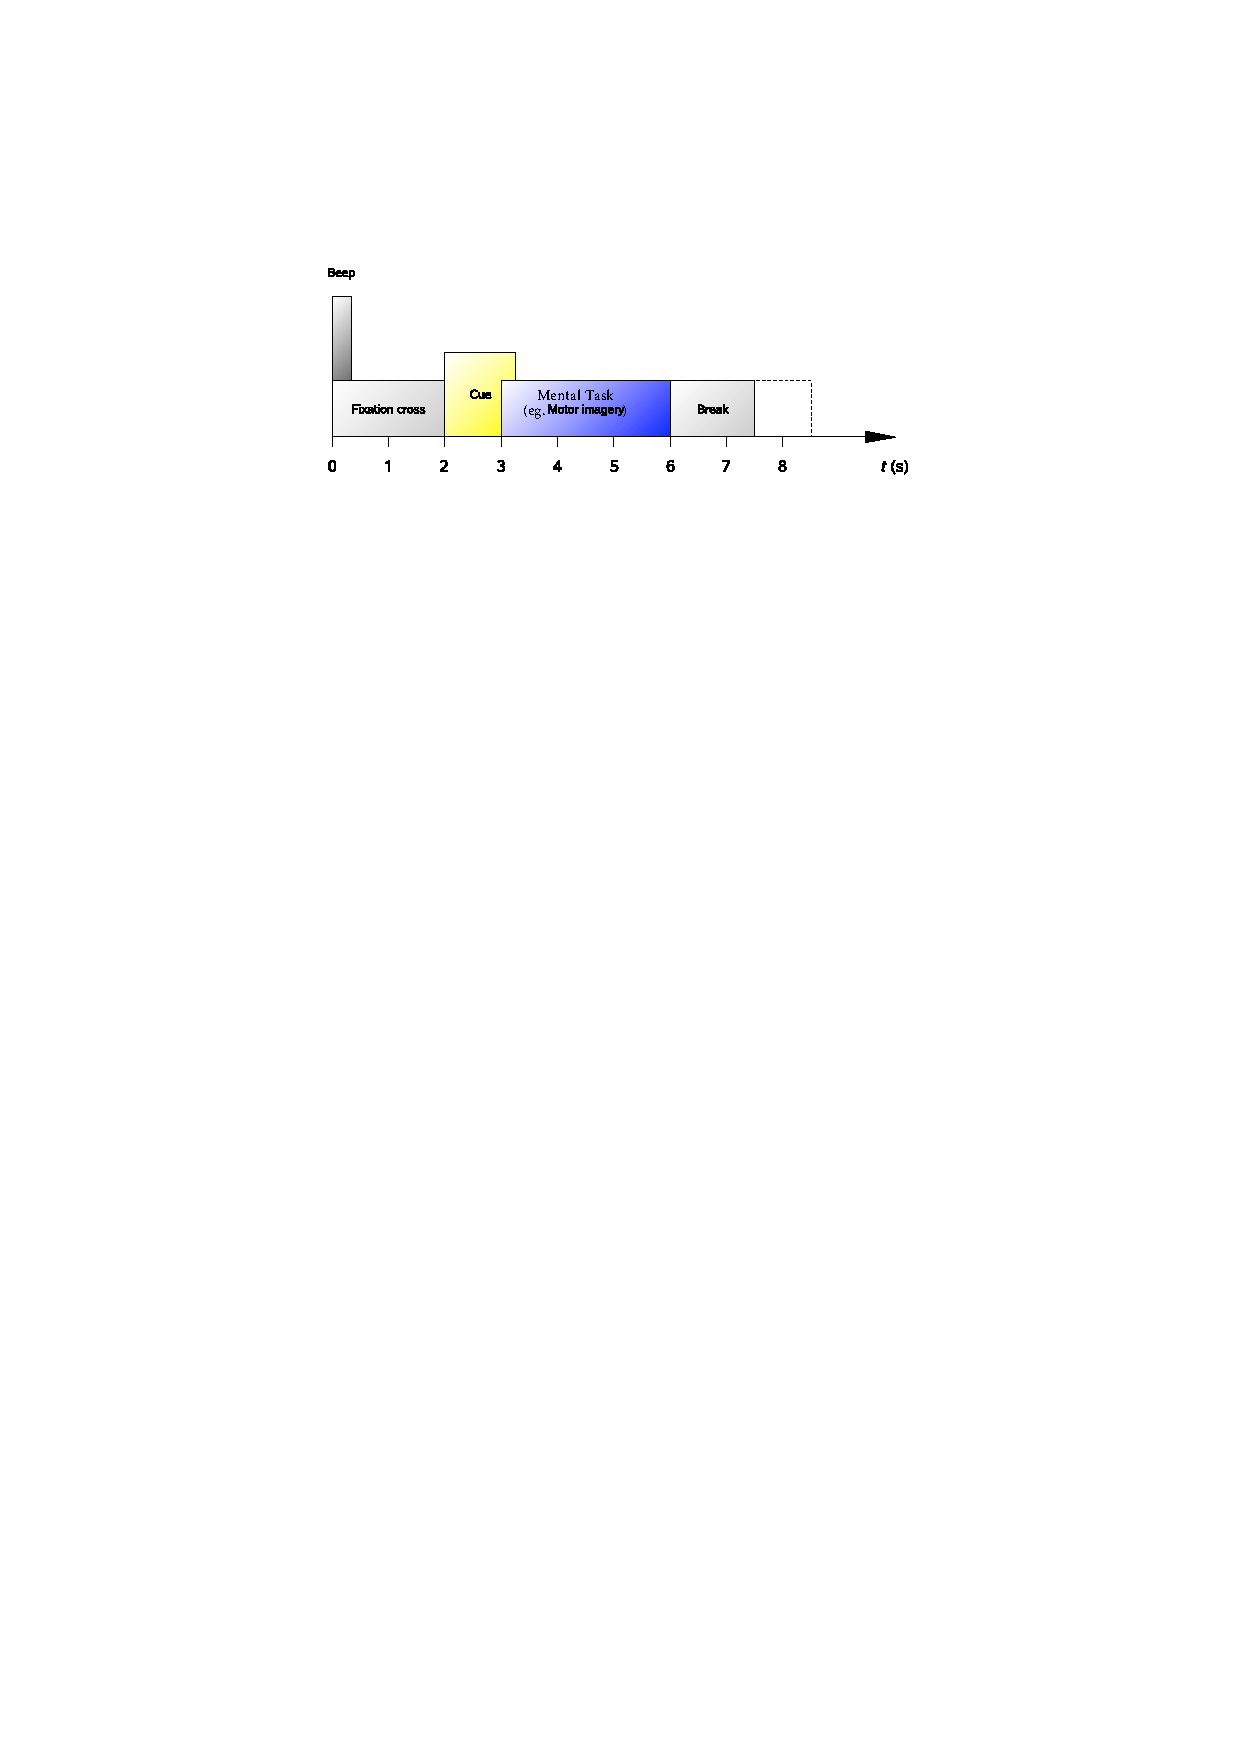
\includegraphics[width=4.0in]{Figures/ERDS-paradigm.pdf}
%    \caption{\footnotesize{Standard ERD/ERS based BCI system paradigm.The
%    break before the next trial should last at least a second to allow the changes in the
%    ongoing EEG/MEG to recover. }}
%    \label{fig:ERDSparadigm}
%\end{figure*}
%\par

\subsubsection{Challenges in ERD/ERS-based BCI systems}

BCIs relying on ERD/ERS face a number of challenges: 
First is the low signal-to-noise ratio. ERD/ERS phenomena are submerged in a much larger brain activity.
It is thus difficult to distinguish a synchronisation or desynchronisation in a single trial. 
%The method used for the quantification of ERD/ERS relies on some kind of averaging methods over many
%trials. BCI systems -- in the signal processing component -- have to enhance
%ERD/ERS and extract the most separable features from a single trial. 
%\par

Secondly, classification into classes representing different intentions is based on the topographical distribution (activated brain regions) and the ERD/ERS frequency range. 
However, as noted, EEG has poor topographical resolution and relatively narrow bandwidth. 
ERD/ERS in ECoG and other signals with better spatial resolution are reported to possess better signal characteristics for classification \citep{wilson_ecog_2006, schalk_brain-computer_2011, power_automatic_2012, naseer_classification_2013, wang_electrocorticographic_2013}. 
Spatial filters are needed to alleviate the poor topographical resolution. 
The impact of spatial filtering on can be seen in \citep{hill_classifying_2006}.

Moreover, ERD and ERS areas are not always the same in different subjects due to physiological differences between them. 
The (de)synchronised frequency band is also not the same amongst subjects. 
Besides, the time where (de)synchronisation happens with reference to a cue is not the same either. 
This forces the BCI systems to identify the relevant brain area (e.g. spatial filter), the frequency band, and the time interval of significant (de)synchronisation \citep{yang_time_2014}. 
The last task becomes even more complex in asynchronous BCI systems where there is no cue, therefore no reference (baseline). 
The term ERD implies that a baseline measured some seconds before the event represents a larger synchronisation \citep{pfurtscheller_event-related_1999}.

A major problem in ERD/ERS-based BCI systems is the user training required. 
Users need to learn how to perform the cognitive tasks such that they can modulate their brain signals in a way that is detectable by the BCI system. 
Even after training, some users still cannot produce signals that are classifiable by the system. This phenomenon is known as \emph{BCI illiteracy} and affects an estimate of 15 to 20\% of BCI users \citep{allison_could_2010}. 
Though the problem of BCI is not exclusive to ERD/ERS BCI, it is more prominent here \citep{hammer_psychological_2012}.
There are many attempts to explain the causes of BCI illiteracy and possible ways of alleviating the problem \citep{allison_could_2010,hammer_psychological_2012,jeunet_why_2016}.

%In terms of information transfer rate, assuming a perfect classification
%accuracy and a negligible processing time, ERD/ERS based BCI systems are
%limited by the minimal length of a trial. As shown in~\ref{fig:ERDSparadigm}, the trial and the inter-trial must be long enough to
%allow event-related changes in ongoing EEG to develop and to recover.

%####################################################################################################################################

\subsection{Event-Related Potential}
\label{subsec:erp}

Event Related Potentials (ERP) are time-locked deflections in the EEG voltage (or electrical activity of a population of neurons) in response to a sensory stimulus. 
A commonly accepted hypothesis is that they are the result of a reorganisation of the phases or changes in specific frequency bands in the ongoing brain signals \citep{pfurtscheller_event-related_1999}.
Having a very small amplitude compared to the ongoing brain activity, they are extracted through an averaging of aligned signal segments of repeated trials. 
After averaging, only the time-locked phenomena will remain, and all unrelated EEG will cancel out. 

The resulting ERP consists of several positive and negative deflections called components of the ERP.
They are designated with a `N' (for negative components) or `P' (for positive components) followed by a number indicating the time when they happened after the stimulus.
Each component reflects a neural process involved in the response to the stimulus.
The first components are usually sensory processes (\textit{i.e.} P120 is the first positive component observed in response to a visual stimulus).
%, N170 reflect the neural processing of face perception). 
They are then followed by more complex processes such as decision, recognition, and emotion related processes. 
N250 reflects the neural processing of a person's own face, P300 reflects the processing of an odd event, N450 marks a processing of conflict, Error Related Potential is negative component observed after an error committed in a selection task \citep{luck_introduction_2014}. 

Only the P300 \citep{polich_updating_2007, donchin_surprise!_1981} and the error related potential (ErrP) \citep{miltner_event-related_1997} components have been explored in BCI applications. 
ERPs are mere responses to sensory stimuli. 
A user would not have a voluntary control of the ERPs and cannot use them as input to a BCI.
The \emph{oddball paradigm} has allowed a ``pseudo'' voluntary control of P300 components, hence its usability in brain-computer interfaces \citep{ritter_averaged_1969}. 
On the other hand, the ErrP has been used in BCI not as a control input, rather as a feedback channel. 
It allows the detection of errors (from the human and the machine) in human-machine interactions \citep{margaux_objective_2012}.   

\subsubsection{P300}
\label{subsubsec:p300}

P300 is a positive deflection in the ERP, typically 300 ms after the perception of an odd event that creates a surprise effect for the subject \citep{donchin_surprise!_1981}.
%The amplitude of the P300 is correlated with the improbability of the discriminated event.
\begin{figure*}[!ht]
    \centering
    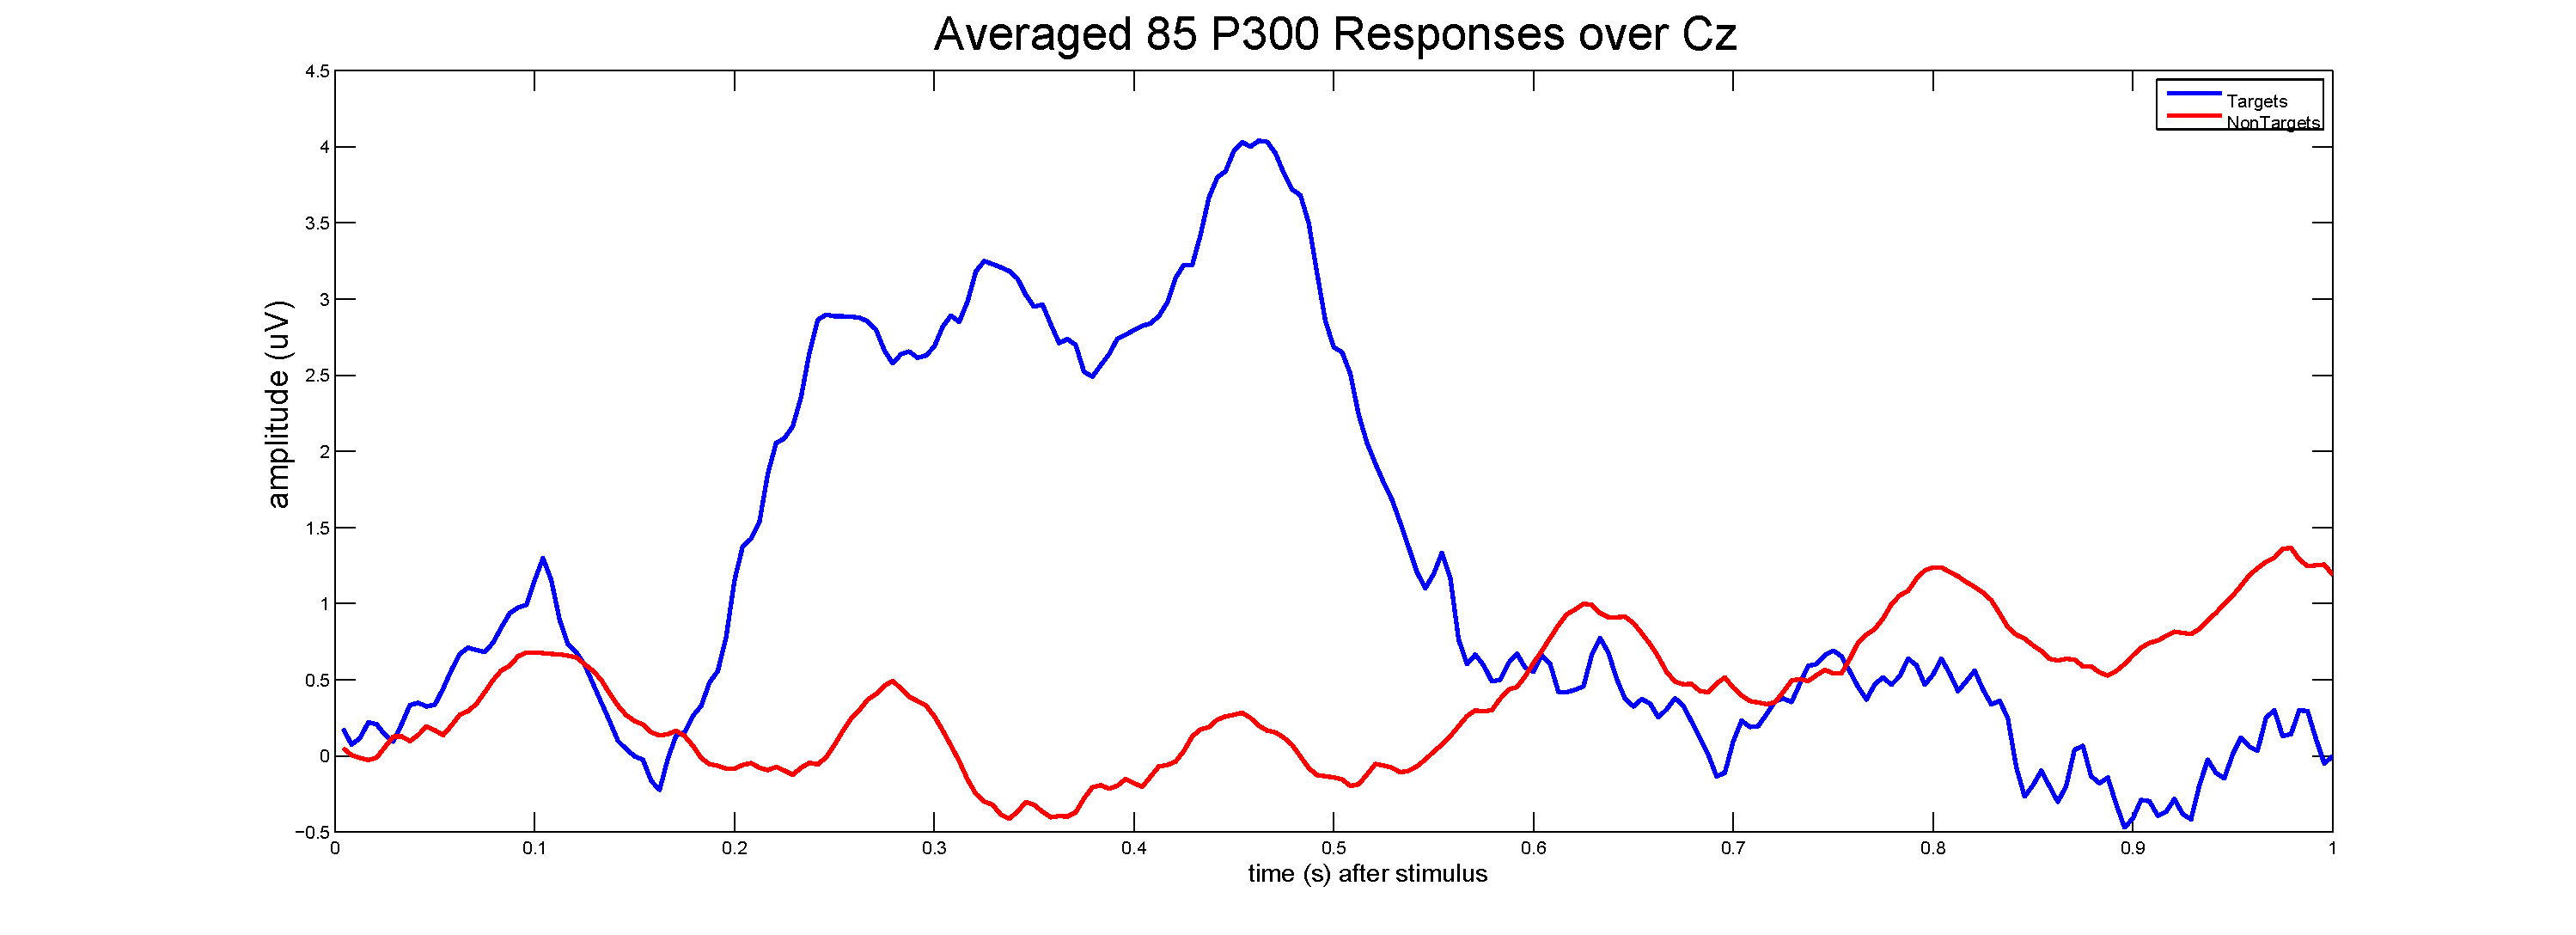
\includegraphics[width=0.5\columnwidth]{Figures/Averaged-85-P300-Responses-over-Cz.pdf}
    \caption{\footnotesize{2550 P300 trials have been averaged to obtain the enhanced P300 (blue line).
    The enhanced P300 is compared to 12750 trials not containing the P300.
    The data used are subject A's recorded signals from the BCI competition III data set II.
    A visual oddball paradigm as described in \citep{donchin_mental_2000} is used to elicit the P300.}}
    \label{fig:85_P300}
\end{figure*}
\par

Contrary to the intuition that P300 might be an exogenous phenomenon, Sutton et al. established that it was endogenous. 
The subject must have perceived the event, analysed it and established its oddity for a P300 to be elicited.
It is related to the psychological reaction of the subject to the stimulus rather than to the physical characteristics of this stimulus \citep{sutton_evoked-potential_1965, sutton_information_1967}.
P300 amplitude is proportional to the temporal probability of the stimulus (e.g. sequential probability) which can roughly be defined as 
($ 1/{\text{total number of stimuli}} $).
It is also, to a lesser extent, related to the stimulus probability: ($\text{stimulus time}/{\text{total trial time}}$) \citep{fitzgerald_temporal_1967}.
\par
P300 has a latency that varies with the difficulty of discriminating the improbable stimulus from the standard ones. 
%For example, while trying to identify, in a series of words, words that are synonymous to ``maverick'', the subject will need some time to process and decide if the word is indeed a synonym, resulting in a longer latency. 
The 300 ms latency is typical in young adults. Older subjects and those with decreased cognitive analogies have smaller P300 with a longer latency. 
Subjects with a greater ability to solve simple problems will generally have shorter latency.
Within the adult population, the latency of P300 increases with age. 
%Polich's review suggests a linear regression of 1.3 milliseconds of latency per year, with a standard error of 31 milliseconds \cite{Polich1991P300inEv}. 
%\par
%The P300 wave is maximally recorded from the midline centroparietal regions. 
%The latency of P300 waves varies from one electrode location to the next, being earlier at more frontal locations. 
Three positive waves overlap during the P300 latency: the P3a near 250 ms, the P3b near 350 ms, and a positive slow wave. 
%The P3a is more frontal than the P3b, while the slow wave is more parietal \cite{Picton1992TheP300}. 
%Depending on the nature of the visual stimulus, the P300 might be larger in the left hemisphere, or larger in the right hemisphere, or just symmetrical \cite{Stapleton1987Endogenous}. 
%When a stimulus was totally unexpected (completely different from the standard stimuli and a new occurrence), the P300 is maximal in the frontal regions \cite{Courchesne1975StimulusNov}.

\subsubsection{P300-based BCI systems}
\label{subsubsec:p300-bci}

In BCI, the \emph{oddball} paradigm is used in a scenario where the subject has a ``pseudo'' voluntary control of P300 generation \citep{ritter_averaged_1969}.  
In this paradigm the subject is presented with a sequence of events that can be classified into two categories, this is the traditional two-stimulus oddball. 
A three-stimulus variation of the oddball paradigm can also be used \citep{polich_updating_2007}. 
In the traditional two-stimulus oddball, events in one of the two categories are rarely presented, thus eliciting a P300. 
%The less probable the eliciting event, the larger the P300 \cite{Donchin2000TheMental}.
\par
Auditory and visual stimuli are used to elicit the P300 with only a few studies focusing on auditory stimuli \citep{elshout_review_2009}. 
Subjects in the complete locked-in state lose all voluntary control and cannot use visual stimuli. 
For such subjects, auditory P300-based BCI could be of great importance. 
Different sounds are played (e.g. notes, words) and for a given task the subject is asked to focus on a particular sound. 
When that sound is played a P300 is elicited around 300 ms later. 
%The BCI system can thus detect the user's intention. Auditory P300s have shorter latency. They typically occur 140 ms earlier than the visual P300. 
Despite the opportunity they represent for people in a complete locked-in state, auditory P300-based BCI have low information transfer rate and have been explored by only a few studies \citep{sellers_p300_2006, elshout_review_2009, kathner_portable_2013, kaufmann_face_2013}.

\par
The most popular application of P300-based BCI systems is the P300 speller \citep{farwell_talking_1988}. 
The subject is presented with a screen, containing a metric of characters. %containing 36 characters arranged in a $6 \times 6$ matrix. 
Rows and columns of the matrix are flashed one after the other in a randomised order. 
The selected character is at the intersection of the row and column which, when flashed, were followed by a P300.
The flashes are repeated several times to enhance the detection of P300 through averaging.
%In another words, when a P300 is generated, the system checks the row or column that was flashed 300 ms earlier. This is repeated a number of time so that both the column and the row of the targeted character are flashed more than once.  
It was pioneered by Farwell and Donchin when for the first time they used the oddball paradigm and the flashing matrix to spell words conveyed to a voice synthesiser. They achieved a communication rate of 12 bits or 2.3 characters per minute \citep{farwell_talking_1988}.
Since then, several improvements have been made. 

\begin{figure*}[!ht]
    \centering
    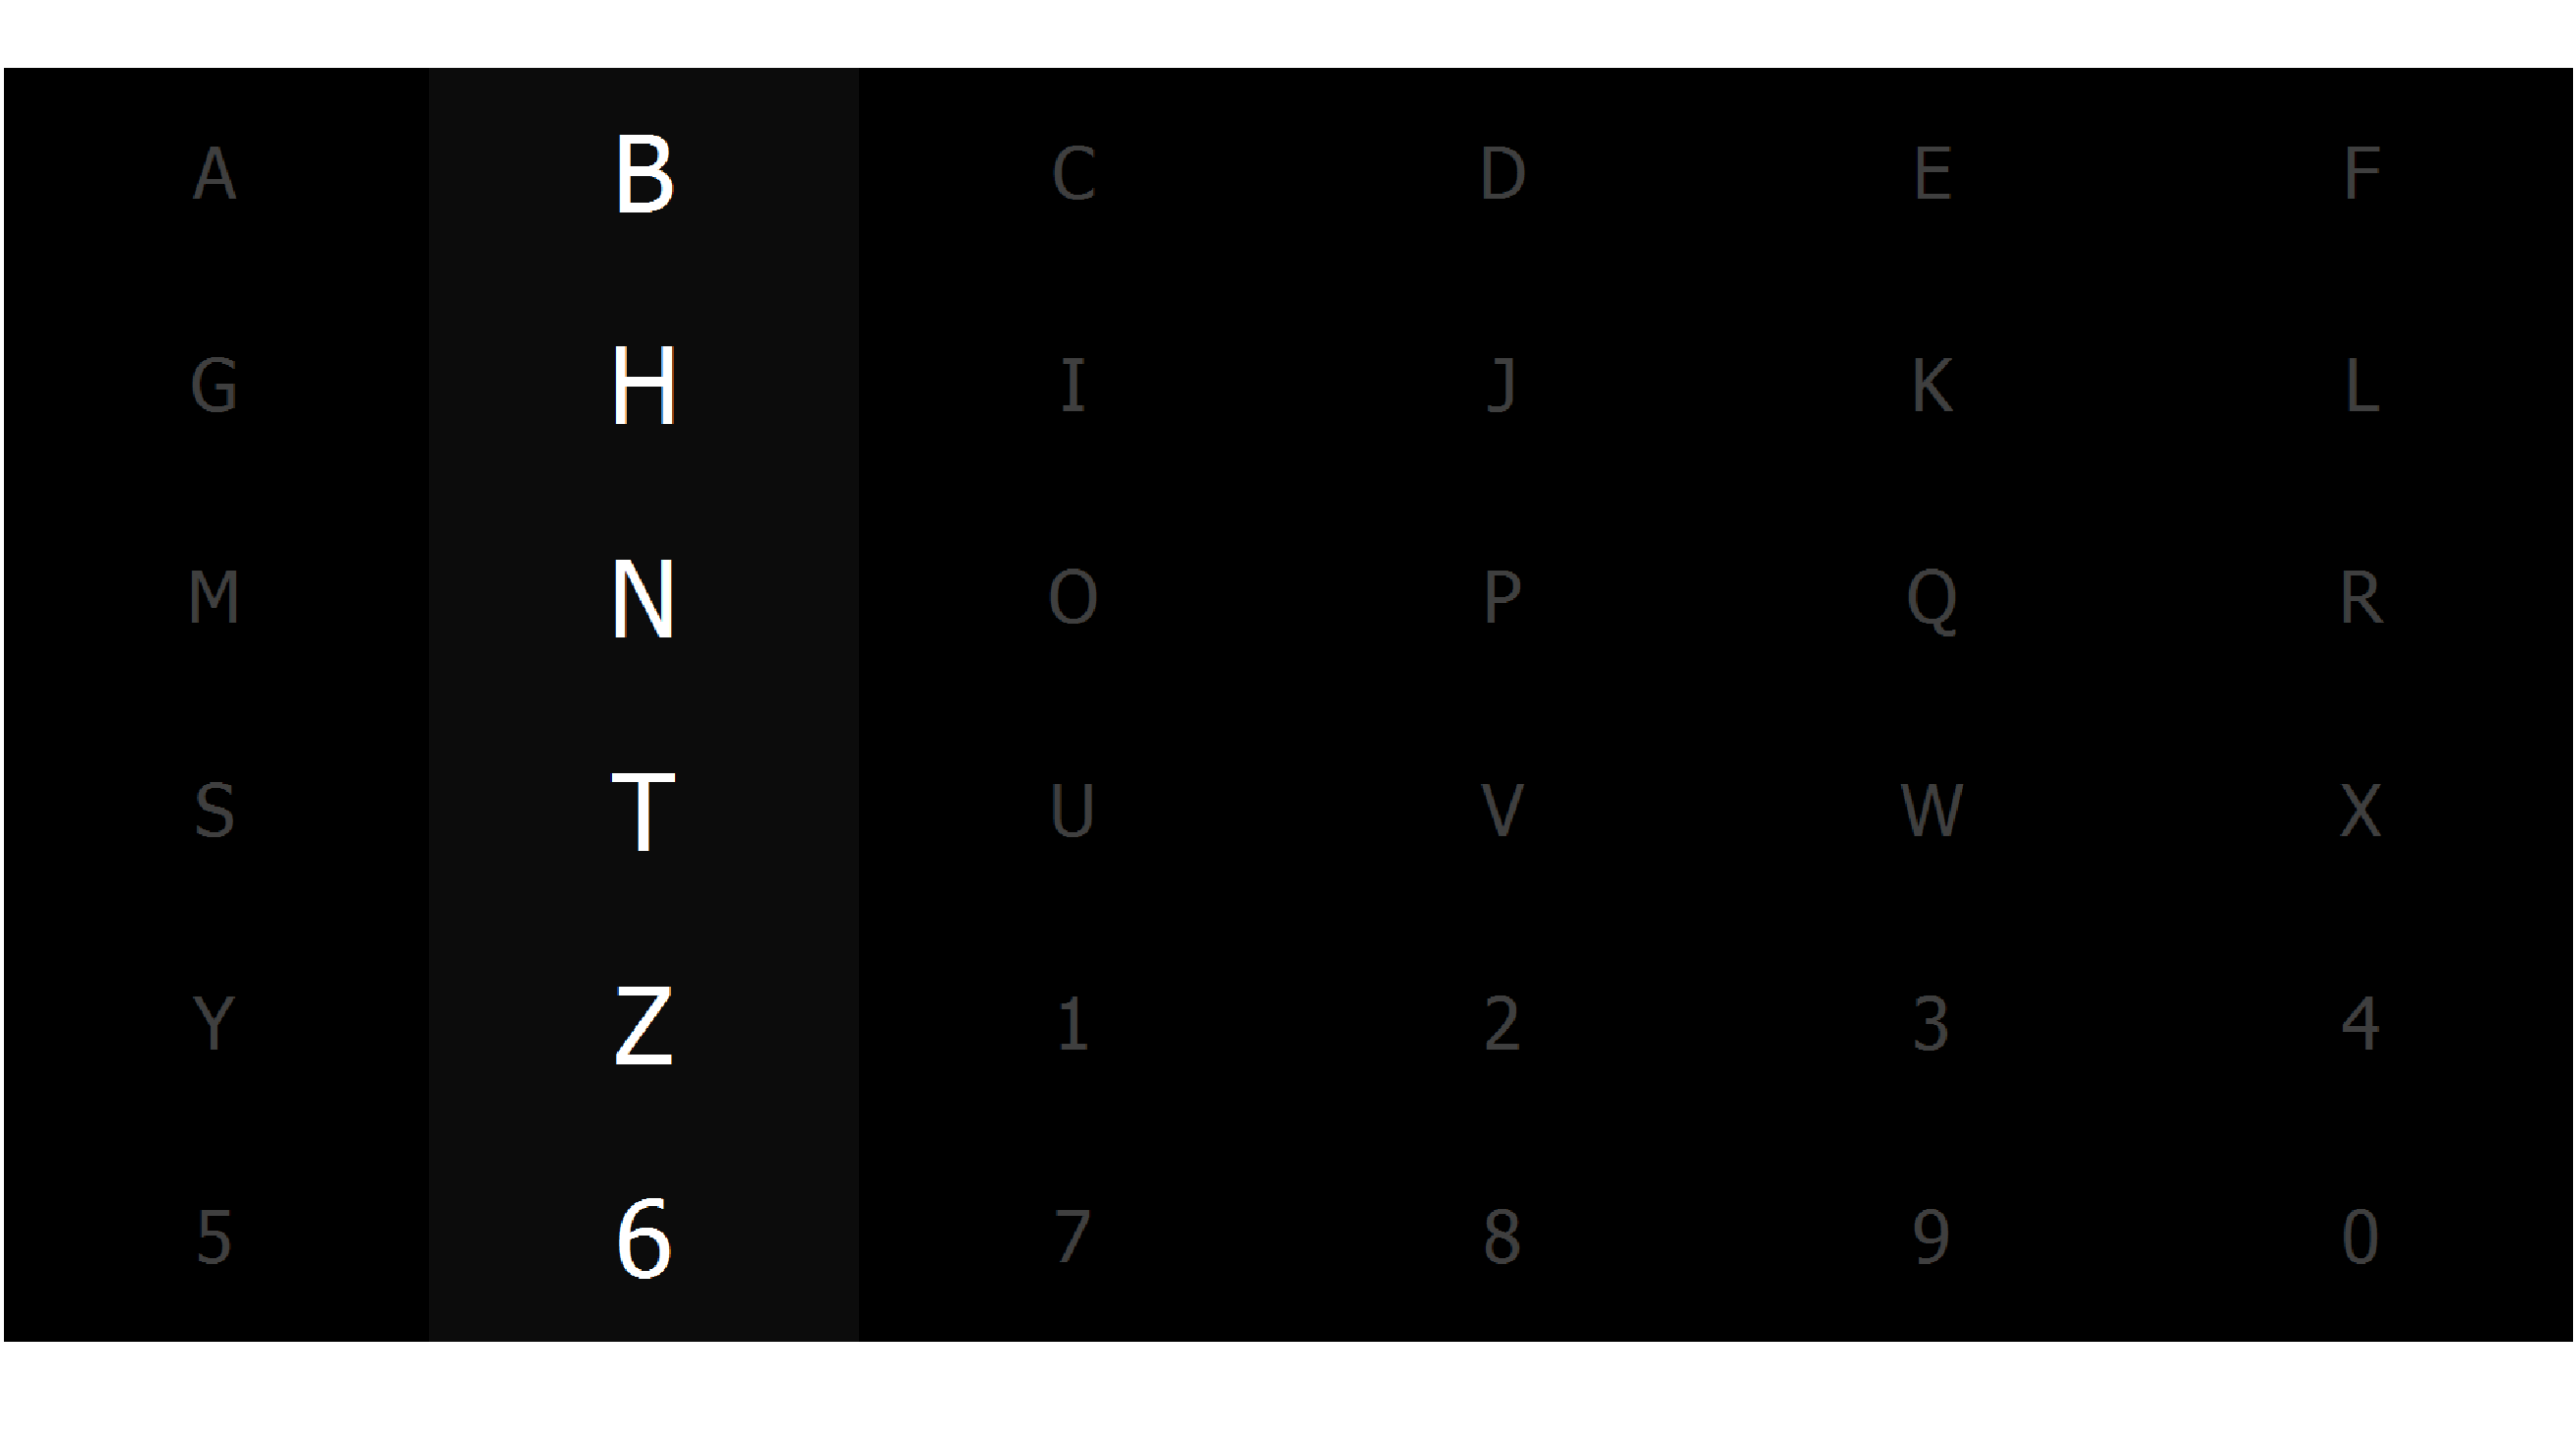
\includegraphics[width=0.5\columnwidth]{Figures/P300Speller.pdf}
    \caption{\footnotesize{A P300-speller screen} }
    \label{fig:P300speller}
\end{figure*}

%Performances were improved by adjusting the size of the stimulation matrix and the duration of the inter-stimulus interval [ref: Sellers 2006], by using the SSVEP evoked by the periodicity of the row/column flashing in the matrix to reinforce the detection of the target symbol.   
A considerable amount of work has been devoted to improving the machine learning algorithms for better detection of P300 \citep{hoffmann_boosting_2005,rakotomamonjy_ensemble_2005,zhang_p300_2007,krusienski_toward_2008,rivet_xdawn_2009,verschore_dynamic_2012,lenhardt_adaptive_2008,panicker_adaptation_2010}.
They have significantly contributed to the development of P300-based BCI.

Other stimulation paradigms, different from the row-column flashing matrix have been proposed, and yield good performances: for example using \emph{chequerboard paradigm} where individual characters are flashed randomly. 
In the chequerboard paradigm flashing objects or human faces improves ERP-based BCI \citep{hoffmann_efficient_2008,kaufmann_flashing_2011,kaufmann_face_2013,chen_survey_2015}. 
%[ref: Hoffmann-2008, ref: Kaufmann-2011-flash, Kaufmann-2013-face, Zhang 2014, Chen-2015-a-survey].

As stated earlier, the detection of P300 is done through averaging of repeated trials. This slows down the communication rate of the BCI.
An important trend in P300 BCI is the detection of P300 in a single trial. This is being achieved by experimental paradigms and signal processing technique that enhance the evoked P300 in a single trial and with adequate machine learning algorithms \citep{bayliss_single_1998,yin_novel_2013,ishita_development_2007,gucluturk_online_2010,kaufmann_comparison_2013} 
%[ref: Bayliss-1998-single, Yin-2013-a-novel-hybrid, Ishita-2007-dev, Güçlütürk-2010-an-online, Kaufmann-2016-comp]. 

Most of P300 BCI systems are synchronous; the timing is dictated by the stimulation system. 
Few implementations of asynchronous P300 BCI have been made. 
It is an effort to discriminate between control state (\textit{i.e.} P300 being elicited) and rest state (\textit{i.e.} the subject does not aim at any target), and to dynamically determine the number of trials needed for P300 detection \citep{lenhardt_adaptive_2008, zhang_asynchronous_2008, schettini_self-calibration_2014}.%, aloise_asynchronous_????} 
%[ref: Aloise-2010-asynch, Schettini-2014-self, Lenhardt-2008-an-adaptive, Zhang-2008-async]. 

Visual P300 stimulation presented thus far requires a gaze control from the subject, which is not achievable by locked-in patients.
A new paradigm was therefore developed to allow the use of visual P300 BCI by locked-in patient. 
%Individual or group of 
One or several characters are presented in a rapid sequence in the middle of a screen. 
In the stream of character, when the intended character is displayed (or magnified), a P300 should be elicited \citep{acqualagna_novel_2010, treder_gaze-independent_2011, aloise_covert_2012,  acqualagna_gaze-independent_2013}. 
%[ref: Acqualagna-2010, Acqualagna-2012, Treder-2011, Aloise-2012-a-covert]. 
Tactile P300 has also been investigated for locked-in patients \citep{kaufmann_comparison_2013}  

\subsubsection{Challenges in P300-based BCI systems}
\label{p300-challenges}

Amongst the limitations in P300-based BCI is the low information transfer rate, due to the repetition of trials required to enhance P300 extraction. 
Acceptable classification is obtained after more than 5 repetitions. 
In \citep{rakotomamonjy_ensemble_2005} for instance 15 repetitions are used and make a trial duration (\textit{i.e.} character epoch) of 35.4 seconds. 
This makes P300-based BCIs very slow. 
Single-trial detection approaches are a solution to this problem, but are hardly achievable. 

\par
The amplitude of the P300 decreases with time. 
The first occurrences of the rare stimuli will elicit a larger P300 \citep{courchesne_stimulus_1975} than the later occurrences will. 
This decrease might be explained by the local versus global probability of the rare stimulus. 
While the local probability of the rare stimuli within an oddball paradigm trial is the same over the entire BCI experiment, their global probability increases, creating a sense of habituation.
In a P300 speller paradigm, this is first observed at the character epoch level as the user gets used to the stimuli that are being repeated, and then over the sessions as the user becomes used to the nature of the rare stimulus. 
The amplitude of P300 will decrease with the habituation, thus deteriorating the BCI performance. 
A potential solution would be to consider the inter-trial variability of the P300 while training the classifier \citep{rakotomamonjy_ensemble_2005}.

\par
On the subject's side, although P300-based BCI systems do not require initial training, they require continuous attention from the user, who should pay close attention to stimuli and notice every time the rare stimulus occurs. 
Over the long run, this might be tiring for some subjects or just not achievable for those with attention disorders \citep{szuromi_p300_2010, krusienski_toward_2008}. 
%All else being equal, improving the methods used in the signal processing component will alleviate the challenges.

\subsubsection{Error-Related Potential}

The neural processing of incorrect response generate a negative going deflection (Ne) in the ERP.
The Ne has been observed in experiences with multiple-choice selection with tasks. Once a person observes an erroneous response, the error-related potential is elicited \citep{gehring_neural_1993}.

The error-related potential could thus improve the performance of non invasive BCI.
The erroneous action can either be automatically corrected or simply undone, as proposed by \cite{margaux_objective_2012}. The erroneous command is automatically replaced by the second most probable output of a probabilistic classifier.  
    
\label{errp}
\goodbreak
%##################################################################################################################################
\subsection{Visual Evoked Potential}
\label{subsec:vep}

%\subsubsection{Steady-State Visually Evoked Potential}

A Visual Evoked Potential (VEP) is an electrophysiological potential in the primary visual cortex in response to a visual stimulus. 
In general, a VEP contains three components illustrated in figure~\ref{fig:VEP}: a negative deflation at around 75 ms from the stimulus referred to as N75, a positive deflation at 100 ms from the stimulus referred to as P100, and a second negative deflation 135 ms after the stimulus called N135.

\begin{figure*}[!ht]
    \centering
    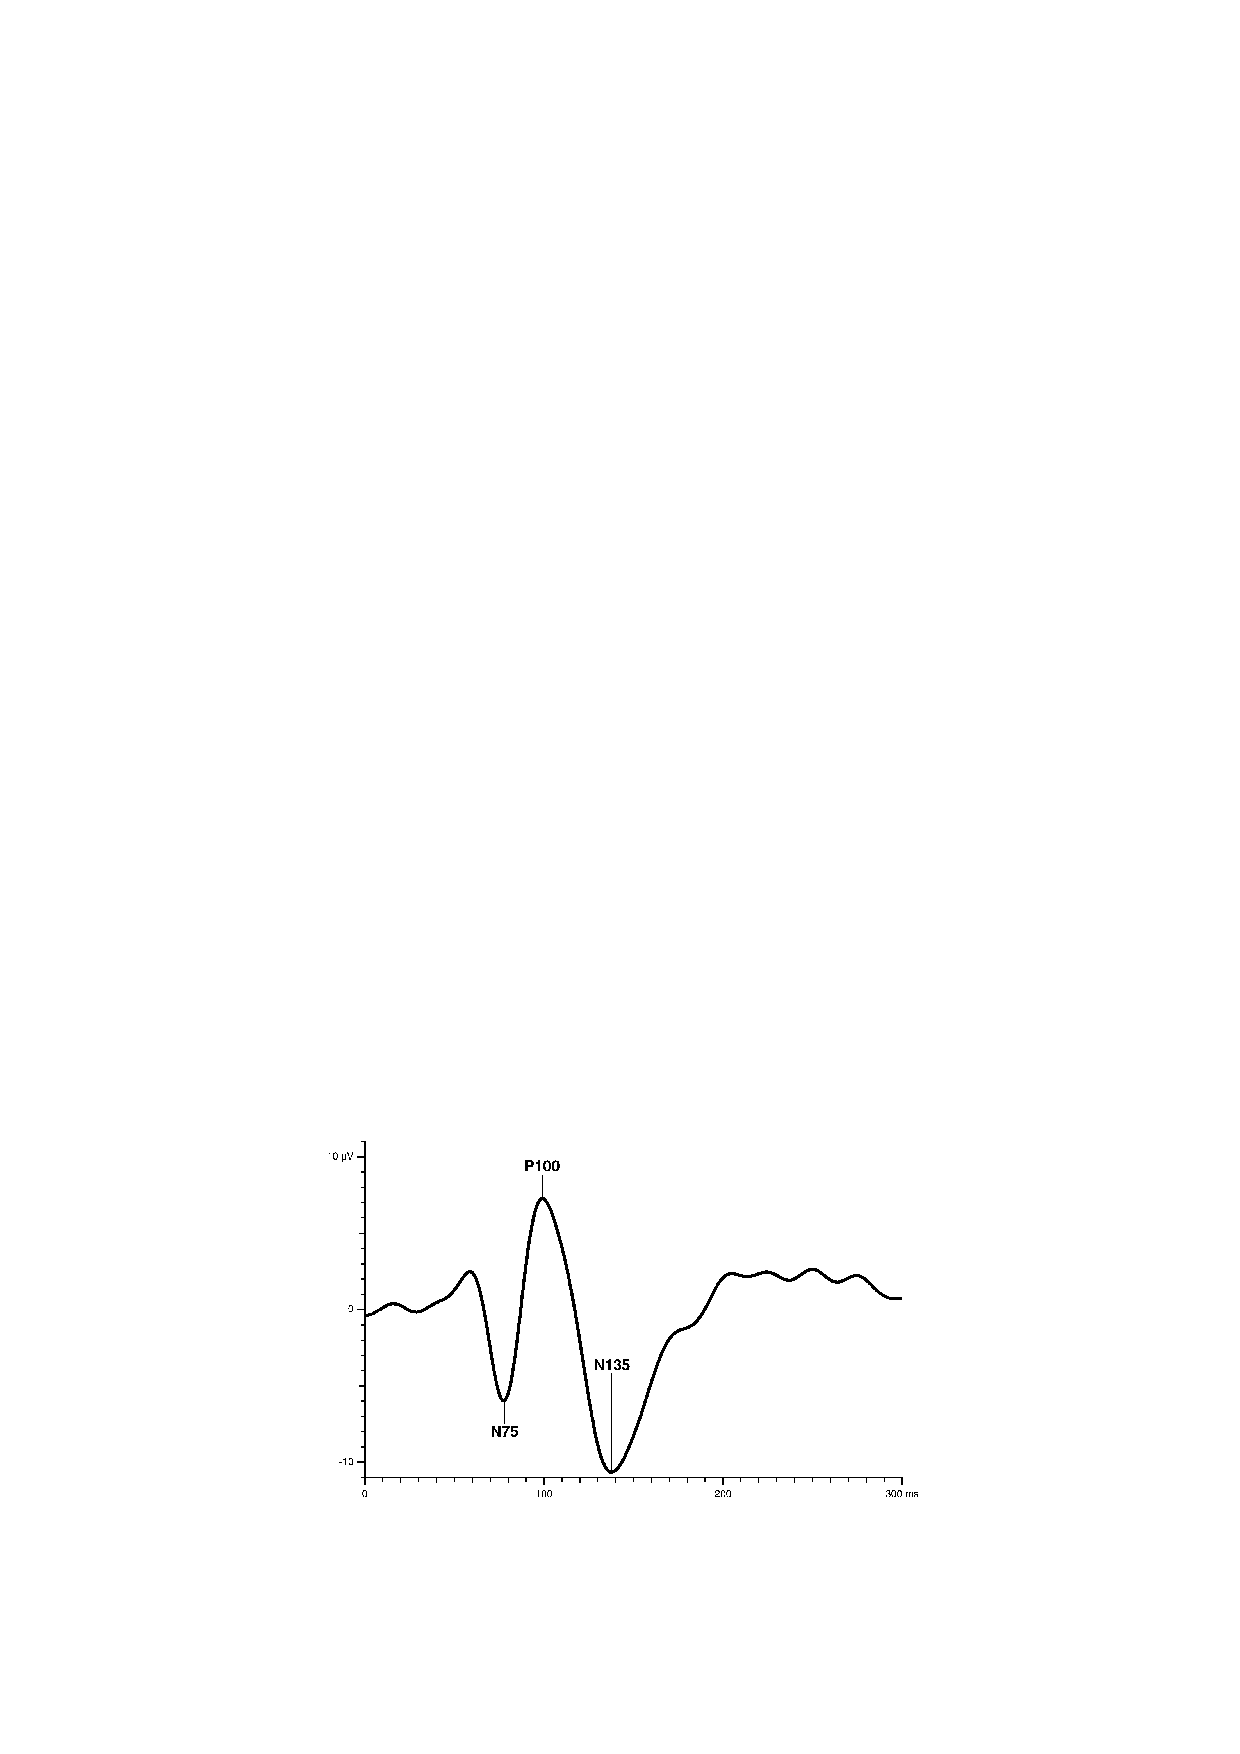
\includegraphics[width=0.5\columnwidth]{Figures/VEP.pdf}
    \caption{\footnotesize{A Standard Visual Evoked Potential} }
    \label{fig:VEP}
\end{figure*}
\par

VEP can be either transient or steady, \textit{i.e.} \emph{Steady-State Visually Evoked Potential} (SSVEP). 
Transient VEP can be defined as the response to an isolated or infrequent stimulus that provides enough time for the system to return to its initial state before onset of the next stimulus.
The steady state response of SSVEP corresponds to a periodic succession of transient evoked potentials \citep{capilla_steady-state_2011}. 
Neuronal activity in the primary visual cortex is synchronised at the stimulation's fundamental frequency and its harmonics. 
This phenomenon is being increasingly used in brain-computer interfaces.  

\begin{figure*}[!ht]
    \centering
    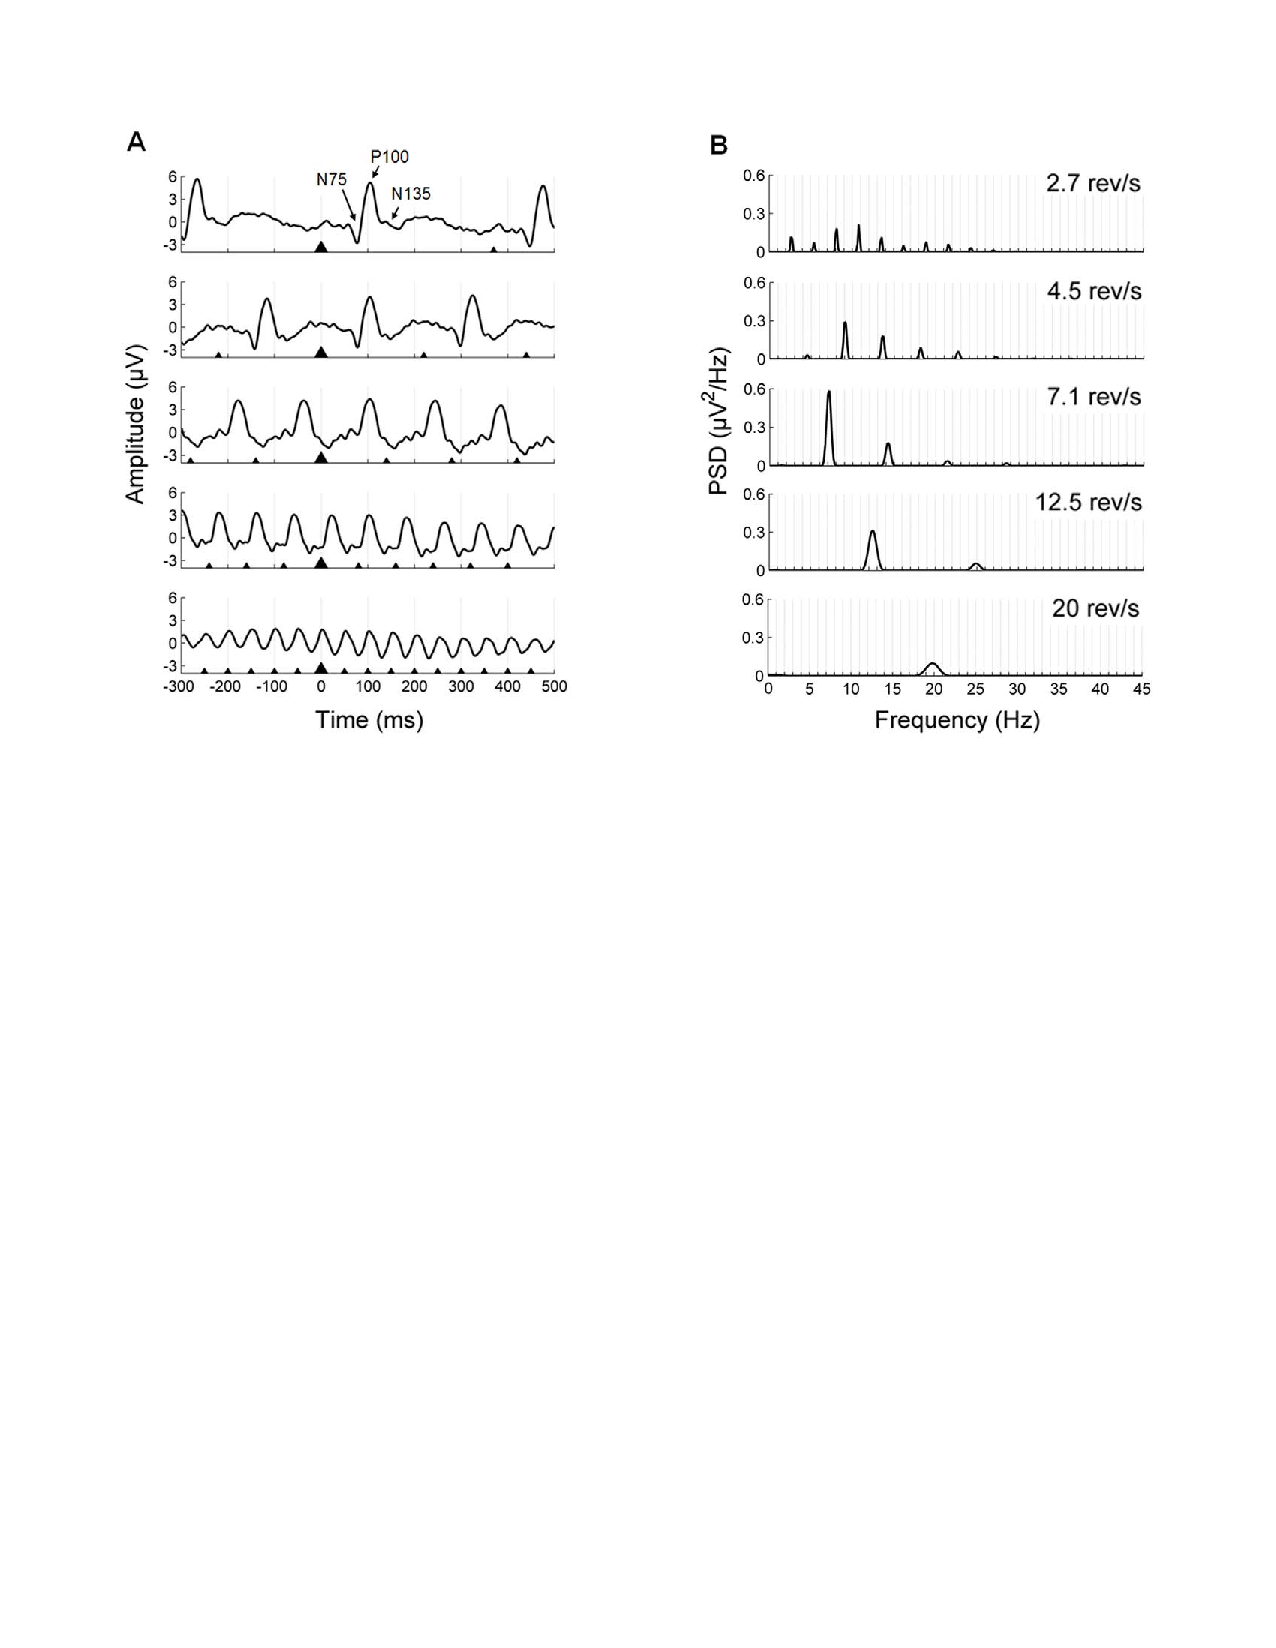
\includegraphics[width=0.5\columnwidth]{Figures/VEP-SSVEP.pdf}
    \caption{\footnotesize{Visual evoked potentials at stimulation frequency of 2.7 Hz, 4.5
            Hz, 7.1 Hz, 12.5 Hz, and 20 Hz. A illustrates the signal in time
            domain and B illustrates the frequency spectrum. \citep[Reproduced from][]{capilla_steady-state_2011} }. }
    \label{fig:VEP-SSVEP}
\end{figure*}
\par

Figure \ref{fig:VEP-SSVEP} is very expressive with regards to the nature of SSVEP. 
While all three major voltage deflation (\textit{i.e.} N75, P100, and N135 ) are observable in steady state responses at lower frequencies (e.g. 2.7 and 4.5 Hz) -- making them very similar to transient evoked responses, they are less visible when the frequency of the stimuli train is increased. 
Only the P100 is still present at all stimulation frequencies. The amplitude of the steady state response appears to be attenuating as the stimulation frequency increases. 
%Based on the conclusion that SSRs are a linear summation of transient responses, 
This attenuation can be explained by latent inhibition, meaning that the transient excitation of the neural generators responding to the first stimulus in a sequence spreads to neurons that, in turn, feed back to them, attenuating the response to an incoming stimulus.
High stimulation frequencies, with periods far shorter than the width of a P100, will suffer more from this inhibition.

\begin{figure*}[!ht]
    \centering
    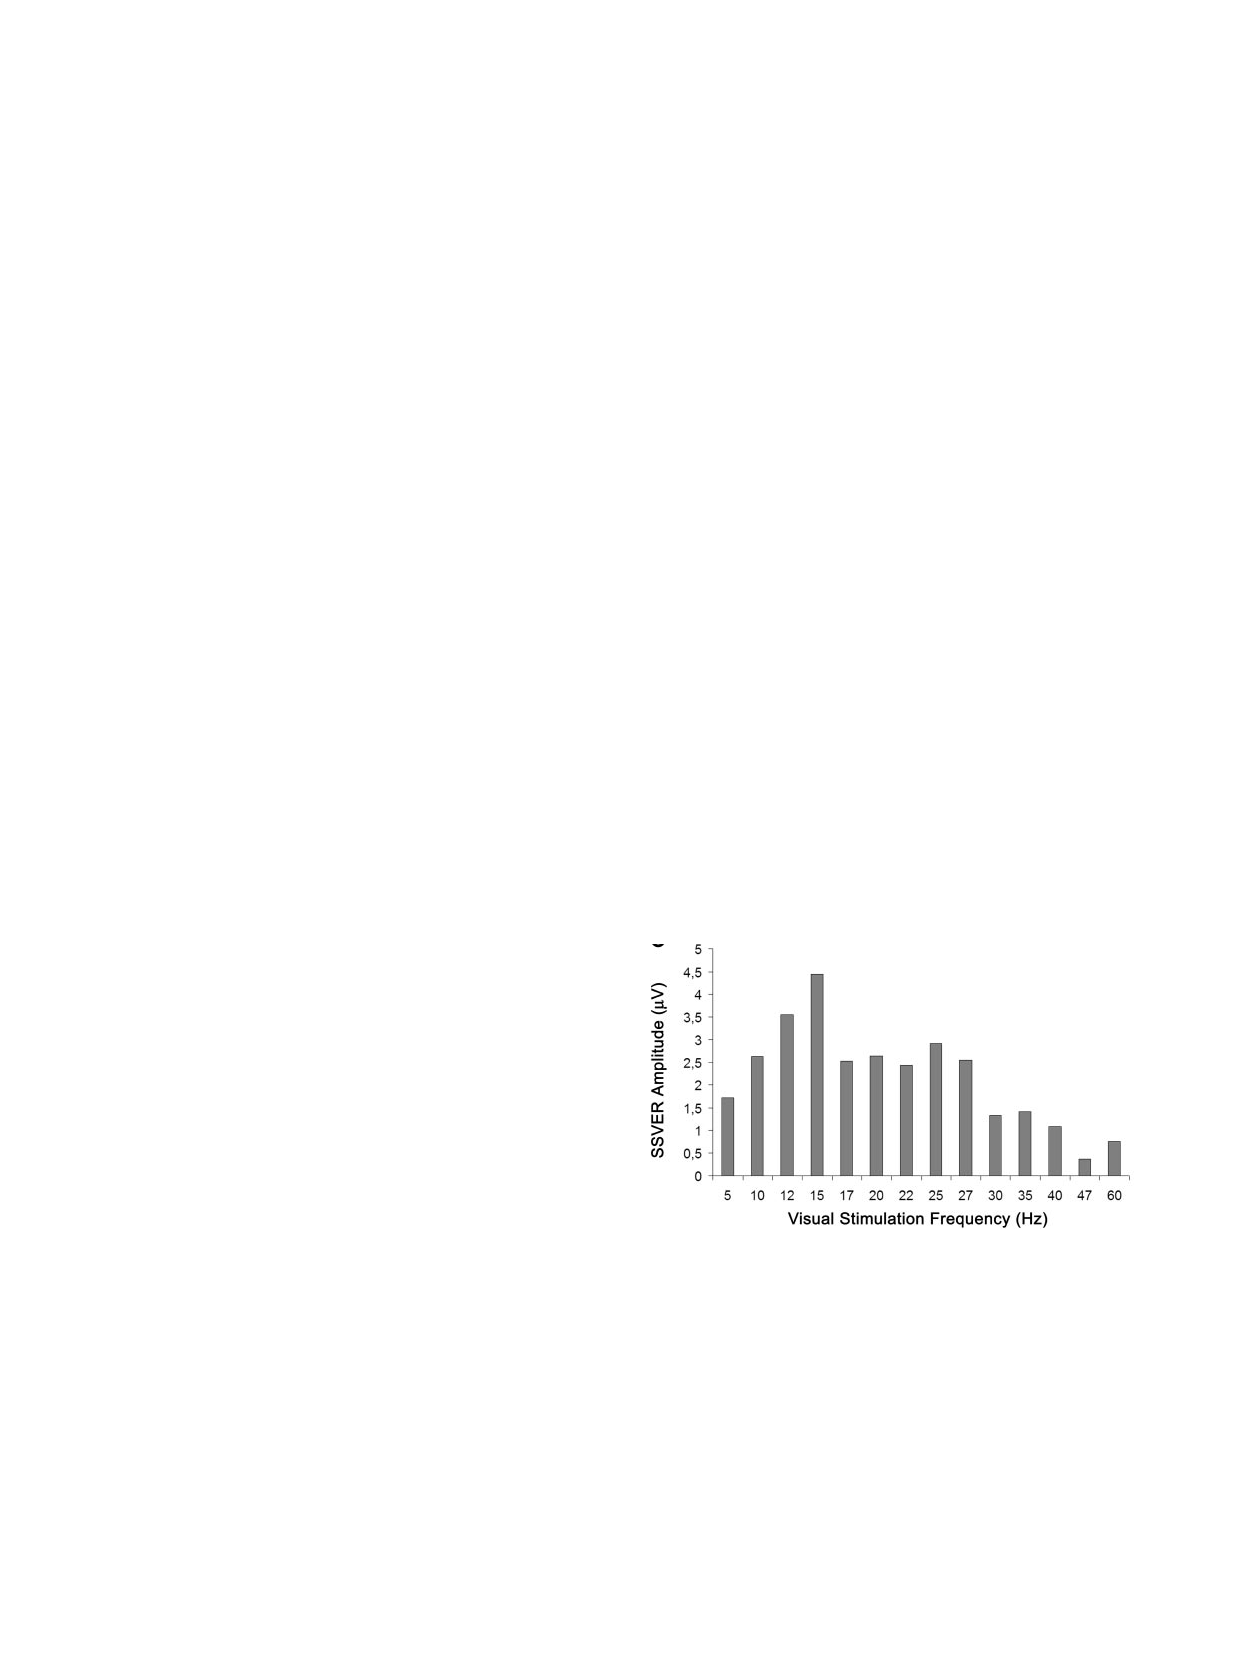
\includegraphics[width=4.0in]{Figures/SSVEP-frequencies.pdf}
    \caption{\footnotesize{Average of the
    mean values of the amplitude of the FFT fundamental frequency of the SSVEP
    recorded at the three occipital leads (Oz, O1, O2) at
    the different stimulation frequencies. The amplitude of the occipital SSVEP,
    expressed in microvolts, reached a maximum at 15 Hz and then fell, with a
    plateau up to 27 Hz, declining at higher frequencies. \citep[Reproduced from][]{pastor_human_2003}.}}
    \label{fig:SSVEP-frequencies}
\end{figure*}
\par

At lower frequencies ( $\le$ 7 Hz), the frequency component corresponding to the stimulation frequency is very weak. 
From 7 Hz up, this component is predominant. 
In both cases, harmonics of the stimuli frequency are visible especially for intermediate frequencies. 
The presence of harmonics is explained by the number of positive and negative voltage deflation found in a single VEP. 
At higher stimulation frequencies, the late deflation of preceding VEP cancel out (or overlap with) the early deflations of the ongoing VEP, leaving out a single VEP component per VEP. 
This explains the absence of harmonics in SSVEP from higher stimulation frequencies. 
With regards to amplitude of response, \cite{pastor_human_2003} reached similar conclusions in their studies. 
They show that responses to low and high stimulation frequencies are less visible than responses to intermediate frequencies (see Figure~\ref{fig:SSVEP-frequencies}). 
Another factor affecting the attenuation of responses to high simulation frequencies is the low pass filtering characteristics of the skull \citep{nunez_electric_2005, bedard_model_2006}.

\subsubsection{SSVEP-based BCI systems}

There are various techniques to design stimulus for SSVEP in BCI. They are reported in \citep{zhu_survey_2010}. 
Different simulation frequencies are used to build multiple BCI commands.
%Two categories of SSVEP stimulation techniques are used in BCI: Pattern stimulus and flash stimulus.
%Pattern stimulus can be divided into two: pattern reversal and pattern onset/offset.
%In pattern reversal stimulation, white and black checks are repeatedly reversing their colours at a specific frequency on a checkboard displayed on a screen. 
%A single reversal perceived by the subject elicits a VEP, while a train of reversals results in SSVEP. 
%For pattern onset/offset a pattern is abruptly exchanged with a diffuse background.
%Pattern reversals are easy to control and offer a noticeable contrast. 
%Flash stimuli on the other side are based on flashing lights. 
%Such stimuli are generated using either light emitting diodes (LED) or screens (\textit{i.e.} LCD orCRT). 
%The amplitude of the evoked potential strongly depends on the nature of the stimulus: its shape, size, color, intensity, contrast with the
%background, etc. 
%This is discussed in more detail in \cite{Zhu2010aSurvey}. %try citep[This is discussed in more detail in]{[ref:}
\par
As in other BCI systems, offline applications of SSVEP-based BCI are used to investigate the parameters influencing the performance of the system. 
SSVEP-based BCI, especially synchronous systems, have the advantage of focusing on EEG activity that occurs at known frequencies. 
Making use of this feature, many studies have reduced the feature extraction methods to a simple frequency spectrum quantification, e.g. Fourier transforms-based methods. 
The target whose stimulation frequency has the largest amplitude in the frequency spectrum of the brain signal recorded in the occipital region is considered to be the one that the
subject is gazing at \citep{muller-putz_control_2008, pfurtscheller_self-paced_2010}. 
Due to inter-trial and inter-subject variability of the frequency spectrum features, parameters optimisation methods are introduced or classifiers such as \emph{support vector machines} that can be trained and used to classify the frequency spectrum features into classes \citep{kalunga_ssvep_2013}.
Methods using canonical correlation analysis are very successful in the identification target's stimulus frequency \citep{lin_frequency_2006, kalunga_ssvep_2013, nakanishi_high-speed_2014}.
\par
Over the past years, interest in SSVEP-based BCI has increased due to the advantages it presents over other BCI systems. 
SSVEP have a higher signal-to-noise ratio, leading to higher classification accuracy, and a fast information transfer rate \citep{nakanishi_high-speed_2014}. 
Moreover, due to the fact that SSVEP is an inherent response of the brain, SSVEP-BCIs' users do not need to go through intensive training.
\par
It should be mentioned that the highest performances have been achieved in synchronous systems. 
Even in some asynchronous systems, the subjects are supposed to be continuously gazing at one target stimulus. 
This keeps the classification simpler as it avoids the complexity of discriminating between intentional control (IC) state and no-control (NC) state.
To alleviate the complexity of having to discriminate continuously between NC and IC, some BCI systems activate the SSVEP target stimuli only when needed.
Once the stimuli are activated, the system is invariably in the IC state, and when deactivated, it is in NC state \citep{cheng_design_2002, pfurtscheller_self-paced_2010}.

SSVEP-based BCI is often employed as a dependent BCI \citep{wolpaw_brain-computer_2000}, that is, some residual muscular capabilities are required to move the eye toward the blinking stimulus as opposed to independent BCI, such as Motor Imagery (MI), where the communication does not rely on any motor capability.
It has been shown that SSVEP could be used as an independent BCI \citep{morgan_selective_1996, muller_feature-selective_2006-1} as the brain oscillations are strongly related to the focus of attention.
Using covert attention, \textit{i.e.} shifting the focus of attention without moving the eyes, subjects can generate different SSVEP responses.%The subjects generate different SSVEP responses without moving their eyes, simply shifting their attention from one stimuli to another.

Visual stimulus plays a crucial role, affecting the BCI performance, and should be designed carefully.
An in-depth review of the literature shows that LED stimuli provide better results than those obtained on computer screen \citep{zhu_survey_2010, oralhan_effect_2016}.
A cognitive study indicates that any stimulation between 2 and 50 Hz induces visible oscillations in the visual cortex \citep{herrmann_human_2001}.
Common values employed in SSVEP studies are between 12 and 25 Hz, as they induce oscillations with higher amplitudes \citep{zhu_survey_2010}. 
One should note that safety of the subject should be taken into account as some frequency ranges of the stimulation could trigger epileptic seizure \citep{fisher_photic-_2005}. 

The phase of the stimulation signal can also be modulated, enhancing the BCI performance by boosting the Information Transfer Rate (ITR) \citep{pan_enhancing_2011, nakanishi_high-speed_2014}. % and a peak bitrate of 124 bit/min~\cite{VOL11}.
An important constraint in that case is that experimental setup requires a synchronization between the display and the recording system, to ensure the correct estimation of the stimulus' phase.
Better alternatives are available when considering systems with such constraints: code-modulated VEP (c-VEP) has yield the highest ITR in BCI \citep{spuler_one_2012, bin_high-speed_2011}.
In c-VEP, the sole difference is that the stimulus flickering is based on pseudorandom sequences instead of the fixed frequencies of SSVEP.

%All these successful approaches in SSVEP and c-VEP rely on CCA.
%Given two sets of signals, CCA aims at finding the projection space that maximises their cross-covariance while jointly minimizing their covariance \cite{Lin2007,kalunga2013ssvep,nakanishi2014high}.
%The common methodology is to find the canonical space between the multichannel EEG trial on the one hand and reference signals, usually sine and cosine of target frequencies and harmonics, on the other hand. 


\subsubsection{Challenges in SSVEP-Based BCI Systems}

Although SSVEP relies on the perception of the subject rather than eye movement, the majority of current SSVEP-based BCI paradigms requires eye movements for the perception of stimuli. 
To operate such systems, the subject must possess a functional visual system which should, moreover, entirely be devoted to the BCI application. 
Nonetheless, studies are investigating the possibility of an SSVEP-based BCI without the need of gazing \citep{lopez-gordo_high_2010}.
\par
%Another challenge is found in the limited number of usable frequencies for SSVEP stimuli.
%While increasing the number of targets in a SSVEP-based BCI is advantageous for the information transfer rate, the number of usable target stimuli is limited. 
This limitation is due to the fact that SSVEP can only be elicited within a limited frequency band. 
Also, due to the fact that harmonics of a stimulation frequency cannot be used in other target stimuli. 
Applications using computer monitors are faced with another limitation in usable frequencies due to the monitors refresh rates. 
The refresh rate must be a multiple of the stimulation frequency to avoid discrepancies in the generated frequency. 
\cite{jia_frequency_2011} proposed a stimuli coding method that combines frequency and phases. 
On a single frequency many stimuli can be coded using different phases, thus increasing the number of targets.
c-VEP is an alternative to SSVEP that does not have this constraint \citep{spuler_one_2012}.
\par
The implementation of asynchronous systems that can discriminate between IC and NC with minimal false positive still poses a challenge. 
This is crucial for real life applications, yet studies investigating the matter and evaluating the performance of such systems are very few in number when
compared to the attention SSVEP-based BCI have drawn in recent years.

\goodbreak
%##################################################################################################################################

\subsection{Discussion}
\label{subsec:neur_pheno_discussion}

The presented neurological phenomena have all been used with considerable success in BCI. 
They each have advantages and drawbacks.
The choice of a neurological phenomenon will depend on the specific needs in the BCI application.
An adequate threshold should be found between the efficiency of the system and the comfort of the BCI user.
Indeed the neurological phenomenon used in the BCI impact both the system's performance and the comfort of users.

In general, there is a duality or complementarity between endogenous and exogenous BCIs, the strengths found in one are usually the weaknesses found in the other.
While exogenous BCIs suffer from the fact that they depend on the muscular functions and on an external stimulus, endogenous BCI are free from this dependency; except visual P300 that might need gaze control.
Endogenous BCIs require that the user be trained, while exogenous BCI can be used with no training.
Endogenous BCI have very low signal amplitude, while their counterpart enjoy a relatively stronger signal amplitude.
Endogenous BCI are flexible; the user can shift between several mental tasks in a single BCI application. That is usually not possible with exogenous BCI.

%Endogenous 	-> pros=>Independent: Muscular system and exteranal stimulus (Exept vP300 that usually require ocular control)
%			-> cons=>Need training: P300 need lesser training 
%				   =>Poor signal amplitude
%Exogenous 	-> pros=>No need for training
%				   =>Good signal to noise amplitude
%			-> cons=>Dependence: Both on muscular and external stimulus

Hence, BCIs that rely on exogenous BCI cannot be used by patients in a complete locked-in state. 
With no muscular function left, they still retain sensory and cognitive abilities that can be leveraged in endogenous BCI.
There is however a vast population of patients who do retain gaze control, for whom visual techniques can still be used. 
Moreover, SSVEP and P300 are related to attention and perception rather than to gaze control. 
An appropriate BCI paradigm leverage this characteristic for their application in locked-in patients.
The dependence to perception and attention also marks the difference between evoked potential-based BCI (\textit{i.e.} P300 and SSVEP) and muscular devices such as eye-trackers, devices that rely on eye-fixation and saccades. 

BCI illiteracy can be observed with any type of BCI.
15 to 20\% of users cannot generate neurological responses necessary to control a particular BCI.
\cite{allison_could_2010-1} discussed the possible causes of illiteracy and proposed few potential solutions that mainly consist of improving BCI accuracy in general. 
An interesting observation is that a subject who is illiterate in one BCI modality (e.g. SSVEP) might effectively use another modality (e.g. ERD). 
Different neurological modalities could be combined in a hybrid interface, where their impact is weighted depending on the user's abilities. 
There are also questions being raised about changing current approaches to BCI altogether.
For example, recently \cite{jeunet_why_2016} challenged the standard training protocol used in MI-based BCI. 
They used the protocol followed in BCI tasks to train users on non-BCI task. They found that about the same rate 17\% of users could not perform the learnt task, which is about the rate of BCI illiteracy. 
Their findings suggest that the training protocol used in BCI is not optimal and might by a influential factor in BCI illiteracy.
These results will surely prompt more digging in approaches used in BCI.

%Une conclusion contenant les conclusin de toutes les section ?
%-------------------------------------------------------------------------
% ------------------------------------------------------------------------
% -*-TeX-*- -*-Hard-*- Smart Wrapping
% ------------------------------------------------------------------------
%%% Literature Survey --------------------------------------------------

%\addtolength{\topmargin}{-.875in}
%\addtolength{\textheight}{.875in}
%\footskip
%\nonumchapter{Literature Survey}
%\chapter{Research Approach}
\chapter[Signal Processing and Machine Learning for BCI]{Signal Processing and Machine Learning for Brain-Computer Interfaces}
\label{chap:lit_survey_sig_process}
\epigraph{It is not by trying to improve the candle that we invented electricity.}{--- \textup{Niels Bohr}}
%-------------------------------------------------------------------------
\section{Signal Processing for Cognitive Functions}
%\subsection{Introduction}
%\label{sec:sig_process_intro}
\label{sec:sig_process}
%* Speak of the EEG processing chain that usually consist of signal preprocessing, spatial filtering, classification.
Brain-computer interfaces translate brain signals into control or communication signal; the signal processing and machine learning component is therefore fundamental.
The usual steps in the translation of brain signals consist of signal preprocessing, feature extraction, and finally a feature classification (or regression).

Signal preprocessing is fundamentally a cleaning up of data. 
The operations involved vary depending on the authors. 
They are usually generic operations such as epoching and removal of non-EEG signal added during the recording. 
\cite{bashashati_survey_2007} report on techniques used to this end.

Feature extraction aims at identifying the characteristics in the EEG signals that bear relevant information for the classification task. 
Thus, it plays an important role in the design and choice of appropriate classifiers. 
The performance of BCI depends as much on the features used as on the classifier.
Feature extraction techniques are a set of operations or transformations applied on the raw EEG such that the neurological phenomenon induced by the BCI task is either enhanced or adequately represented. 
From the EEG signal they can extract:
\begin{itemize}
\item  time features e.g. EEG signal amplitudes, signal power \citep{rivet_xdawn_2009},
\item frequency features e.g. band power, power spectral density \citep{bhattacharyya_performance_2010}, 
\item parametric features e.g. Auto Regressive (AR) and adaptive AR (ARR) parameters \citep{zhang_classification_2015}, 
\item time-frequency features e.g. wavelet transforms \citep{kumar_design_2010, dingyin_feature_2011, zhang_comparison_2015}, short-time Fourier transform \citep{kumar_design_2010}, empirical mode decomposition \citep{gaur_empirical_2015, wang_motor_2011,liu_novel_2011}, 
 \item spatial features e.g. Independent Component Analysis (ICA) \citep{wang_enhancing_2006, wang_improving_2013, brunner_spatial_2007}, Common Spatial Patterns (CSP) \citep{ang_filter_2012, barachant_common_2010, blankertz_optimizing_2008}, Canonical Correlation Analysis (CCA) \citep{nakanishi_high-speed_2014, kalunga_ssvep_2013}, Principal Component Analysis (PCA) \citep{kottaimalai_eeg_2013, yu_analysis_2014}, xDAWN \citep{rivet_xdawn_2009}.
\end{itemize}
Detailed reviews of classic feature extraction methods can be found in \citep{lotte_review_2007, nicolas-alonso_brain_2012, bashashati_survey_2007, khorshidtalab_eeg_2011, krusienski_critical_2011}. 
The choice of feature extraction techniques is guided by the neurological phenomenon used in the BCI.
For instance, in SSVEP, relevant information will be contained in the spectral features while in P300, temporal features will suffice. 
\cite{fukunaga_introduction_1990} defines feature extraction for classification as a search, among all possible singular transformations, for the best subspace which preserves class separability as much as possible in the lowest possible dimensional space.

Spatial filters (from which spatial features are extracted) have proven to be successful tools in extracting (or enhancing) the neurological phenomenon from the EEG signal. 
The information of interest is hidden in the recorded EEG, a mixture of simultaneous active brain sources and noise sources in the recording environment. 
The signal of interest could be overlapped in time, space, and frequency with multiple signals. 
Using \textit{a priori} knowledge on the phenomenon of interest 
%(\textit{i.e.} unsupervised methods)
 or knowledge deduced from pre-recorded data, spatial filters extract better signal features that make subsequent processing tractable. 
Supervised and semi-supervised approaches lead to highest classification performances.
Once a spatial filter has been applied to EEG data, any feature extraction technique can further be used merely for feature representation. 
%Their effect is trivialised by the spatial filter.

With relevant features, standard classification algorithms such as Linear Discriminant Analysis (LDA) and Support Vector Machine (SVM) \citep{rivet_xdawn_2009, pfurtscheller_self-paced_2010, spuler_one_2012}, Artificial Neural Networks \citep{haselsteiner_using_2000, sturm_interpretable_2016}, Quadratic Discriminant Analysis \citep{friedman_regularized_1989, bhattacharyya_performance_2010}, Hidden Markov Model \citep{obermaier_hidden_2001, lee_pca+hmm+svm_2003, yan_classifying_2008}, and nearest neighbour \citep{cincotti_comparison_2003, schlogl_characterization_2005, bhattacharyya_performance_2010} can be applied.

The signal processing pipeline can be represented as in Figure \ref{fig:processing_pipeline}. 
Removing the preprocessing and the feature representation phases that do not require training, the machine learning pipeline of most successful BCI systems \citep{ang_filter_2012, spuler_one_2012, rivet_xdawn_2009} consists mainly of spatial filtering and classification/regression blocks.

\begin{figure}[!h]
\centering

\includegraphics[width=0.8\columnwidth]{Figures/processing_pipeline}
\caption{BCI signal processing pipeline. The fundamental blocks for machine learning are in blue (\textit{i.e.} spatial filtering and classification). Filters and classifiers are learned from training data. Gray blocks (\textit{i.e.} preprocessing and feature representation) do not require learning. }
\label{fig:processing_pipeline}
\end{figure}
Spatial filters and classifiers are trained offline on pre-recorded data. 
The best preprocessing and feature representation can be chosen based on the offline analysis through cross validation. 

Hereafter, classical couplings of spatial filters and classifiers are illustrated as they are used in machine learning of various BCI types \textit{i.e.} motor imagery, P300, and SSVEP.   

Filtering is based on a modelling of EEG as a linear mixture of multiple neural ensembles to which noise is added:
\begin{equation}
\X = AS+R
\label{eq:eeg_model}
\end{equation} 
where $\X \in \Re^{\dc \times \dt}$ is the EEG recorded on $\dc$ channels over $\dt$ samples, $S \in R^{K \times \dt}$ are the brain sources, $A \in \Re^{\dc \times K}$ is a matrix defining the mixture of the brain sources, and $R \in \Re^{\dc \times \dt}$ is the additive noise, with $\dc \leq K$.  
Spatial filters are designed to extract signal of interest \eqref{eq:eeg_model} based on \textit{a priori} knowledge on the neurological phenomenon of interest or knowledge deduced from pre-recorded data.

%* In each method provide: Brief expllanation, Equations, graphical example (if possible), example of applications (+progress) in BCI
%* Organise these methods per BCI type (ERD, ERP, SSVEP)
%- ICA
%- PCA
%
%I. ERD-ERS (MI)
%- CSP, SVM, LDA, ANN
%II. ERP
%- xDawn
%III. SSVEP
%- CCA, SVM, LDA, ANN
%
%- SVM 
%- LDA
%- ANN
%

\subsection{Motor Imagery Processing} % (ERD/ERS based BCI)}
\label{subsec:sign_proc_mi}
%CSP/LDA
Common Spatial Patterns are spatial filters that has been particularly designed for motor imagery tasks classification \citep{koles_spatial_1990}. 
CSP extracts EEG spatial components that are common to two imagery tasks, but maximising the variance of the signal recorded during one task while minimising the variance in the other task.
The distribution of filtered samples belonging to one imagery task has maximal variance, while the distribution of samples in the other task has minimal variance, or vice-versa as illustrated in Figure \ref{fig:class_scatter_csp}. 
CSP should capture the contralateral effect of ERS versus ERD induced by motor imagery tasks. 

CSP has been successfully coupled with linear discriminant analysis classifiers \citep{dornhege_increase_2004, popescu_single_2007}. 
Indeed like CSP, LDA also relies on data class scatter. 
LDA projects samples into a space where the within-class covariance matrices are minimised, while the between-class covariance matrix is maximised. Here the covariance matrices are proportional to the class scatter.  

\subsubsection{Common Spatial Patterns}

CSP model is given by:
\begin{equation}
\label{eq:csp}
S = WX
\end{equation}
%Given the model given in equation \eqref{eq:eeg_model}, 
CSP finds the filter $W \in \Re^{\dc \times \dc}$ that minimises the variance of the filtered signal $S$ in one condition and maximises it in the other.
\begin{figure}[h!]
\centering
\subfigure[]{
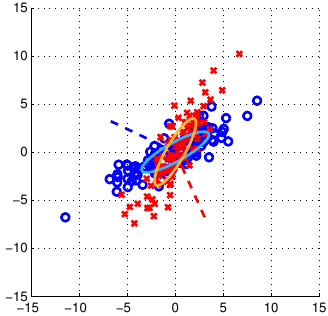
\includegraphics[width=0.4\textwidth]{Figures/class_scatter_before_csp}
\label{fig:class_scatter_before_csp}
}
\subfigure[]{
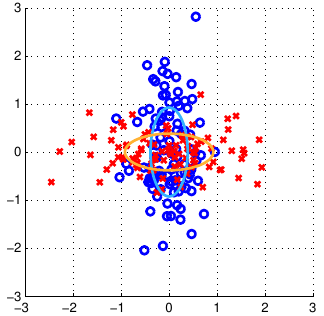
\includegraphics[width=0.4\textwidth]{Figures/class_scatter_after_csp}
\label{fig:class_scatter_after_csp}
}
\caption{CSP effect on class distribution. 
CSP is applied on a 2D toy data set containing samples from two classes marked with red crosses and blue circles. 
(a) Samples distribution is shown before CSP filtering. The ellipses show estimates of each class covariance. 
It can be seen that the two classes are highly correlated. 
The dashed lines show the direction of the CSP projections $\mathbf{w}_j$ ($j=1,2$). 
(b) Distributions after CSP projections. The two distributions are orthogonal, showing that the two classes are uncorrelated. 
Each axis gives the largest variance in one class and the smallest in the other. \citep[Image from][]{blankertz_optimizing_2008}.} 
\label{fig:class_scatter_csp}
\end{figure}
Neglecting additive noise in Equation~\eqref{eq:eeg_model}, the CSP model is equivalent to finding the inverse of $A$:
$W = A^{-1}$. 
In EEG modelling, $A$ is called the \emph{forward model} or the \emph{mixing matrix} and $W$ the \emph{reverse model} or \emph{de-mixing matrix}.  
$A$ describes the spatial pattern. 

Let $\X_i \in \Re^{\dc\times \dt}$ be a band-pass filtered signal of EEG recorded at epoch $i$.
An estimate of its covariance matrix $\cov{i} \in \Re^{\dc\times \dc}$ can be computed as:
\begin{equation}
\label{eq:covmat1}
\cov{i} = \frac{\X_i \X_i^{T}}{trace(\X_i \X_i^{T})} 
\end{equation} 
A class covariance matrix is obtained as: 
\begin{equation}
\cov{(c)} = \frac{1}{N_c} \sum_{i=1}^{N_c} \cov{i}
\end{equation}  
In a two imagery task, $c \in \left\lbrace +,- \right\rbrace$, and $N_c$ is the number of epochs in class $c$. 
\\CSP solves the following problem:

\begin{equation}
\label{eq:csp_problem}
\begin{aligned}
& \underset{W}{\text{maximise}}
& & \mathrm{trace}(W^T \cov{(+)} W) \\
& \text{subject to}
& & W^T(\cov{(+)} + \cov{(-)})W=\eye.
\end{aligned}
\end{equation} 
\begin{figure*}[!th]
    \centering
    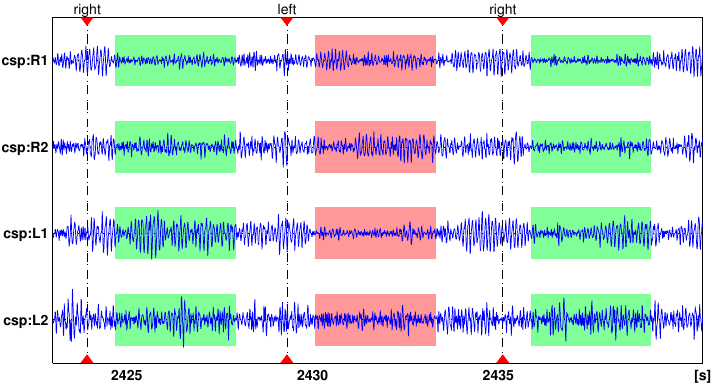
\includegraphics[width=0.8\columnwidth]{Figures/csp_effect}
    \caption{\footnotesize{Effect of CSP filtering. A continuous EEG signal containing two right-hand imagery epochs and one left-hand imagery is filtered using four CSP filters ($\mathbf{w}_j$): csp:R1, csp:R2, csp:L1, and csp:L2. The resulting signals from csp:R1 and csp:R2 have large variance during left hand imagery, while signals from csp:L1 and csp:L2 have large variance during right hand imagery. \citep[Image from][]{blankertz_optimizing_2008}.} }
    \label{fig:csp_effect}
\end{figure*}
The constraint in \eqref{eq:csp_problem}, where $\eye$ is the identity matrix, forces $W^T \cov{(-)} W$ to be minimal when $W^T \cov{(+)} W$ is maximal. 
There are many ways of solving this problem. A simple way is to solve it as a generalised eigenvalue problem \citep{koles_spatial_1990, blankertz_optimizing_2008}:
\begin{equation}
\label{eq:csp_gen_eigen}
\cov{(+)} \mathbf{w}= \lambda \cov{(-)} \mathbf{w} \, ,
\end{equation}
where $\mathbf{w}_j$ ($j=1, \dots, \dc$) are the generalised eigenvectors that constitute the vectors of the matrix $W$, and $\lambda_j = \lambda_j^{(+)}/\lambda_j^{(-)}$, with $\lambda_j^{(c)} = \mathbf{w}_j^T \cov{(c)}\mathbf{w}_j$ where $0 \leq \lambda_j^{(c)} \leq 1$ and $\lambda_j^{(+)} + \lambda_j^{(-)} = 1$. 
$\lambda_j^{(c)}$ is the variance in the filtered signal $\mathbf{s}_j = \mathbf{w}_j^T X$ in the epochs corresponding to class $(c)$.
Thus filtering (\textit{i.e.} projecting) the EEG signal $X_i$ with $\mathbf{w}_j$ that corresponds to the largest $\lambda_ j^{(+)} \rightarrow 1 $, will maximise the variance in class $(+)$ while minimising it in class $(-)$ as illustrated in Figures \ref{fig:csp_effect} and \ref{fig:class_scatter_csp}.

This discussion of CSP is limited to two-class motor imagery. The application of CSP has been extended to multi-class cases \citep{dornhege_increase_2004, grosse-wentrup_multiclass_2008}.

\subsubsection{Linear Discriminant Analysis}

Given a set of $n$ $\dc$-dimensional samples $\x_1, \x_2, \dots, \x_n$ ($\x_i \in \Re^\dc$) , LDA finds a lower dimensional space (typically $\dc-1$) where the data are the most separable.
In a two-class case ($c \in \left\lbrace +, - \right\rbrace$), $n_{(+)}$ samples belong to the positive subset $\mathcal{X}^{(+)}$,
and $n_{(-)}$ samples belong to the negative subset $\mathcal{X}^{(-)}$
LDA finds a projection vector $\w$ that will achieve the mapping
\begin{equation}
y = \w^T \x
\end{equation}
that obtains the $n$ $(\dc-1)$-dimensional samples $y_1, \dots, \y_n$ ($y_i \in \Re^{d-1}$), where the positive subset of the projected data $\mathcal{Y}^{(+)}$ is separable from the negative subset $\mathcal{Y}^{(-)}$.
If the original $\dc$-dimensional samples are highly overlapped, not even the best $\w$ could separate them in a lower dimension. 
A successful application of CSP will avoid such problems.

For separability brings the idea of distance between subsets,
LDA uses the difference of projected samples means:

\[ |\tilde{\m}_{(+)} - \tilde{\m}_{(-)} | \] 
If $\m_{(c)}$ is the $\dc$-dimensional class mean,
\begin{equation}
\label{eq:lda-class-orig-mean}
\m_c = \frac{1}{n_{(c)}} \sum_{\x \in \Xc^{(c)}} \x,
\end{equation}
$\tilde{\m}_{(c)}$ is the mean of projected samples belonging to $\Yc^{(c)}$ and is given by  
%\begin{equation}
%\tilde{\m}_c = \frac{1}{n_{(c)}} \sum_{y \in \mathcal{Y}^{(c)}} y
%\end{equation}
\begin{equation}
\label{eq:lda-class-proj-mean}
  \begin{split}
    \tilde{\m}_{(c)} & = \frac{1}{n_{(c)}} \sum_{y \in \Yc^{(c)}} y
		\\
    & = \frac{1}{n_{(c)}} \sum_{y \in \Yc^{(c)}} \w^T \x = \w^T \m_c ,
  \end{split}  
\end{equation}
Maximising the distance between class means does not ensure class separability. 
If both subset are very scattered, their samples can still be highly overlapped even when their respective means are very distant.
This introduces a second criterion in LDA: the distance between class means should be large relative to the \emph{within-class scatter} given by:
\begin{equation}
\label{eq:lda-within-class-scatter}
\scat_{(c)} = \sum_{y \in \Yc^{(c)}} (y-\tilde{\m}_{(c)})^2  
\end{equation} 
The total within-class scatter is $\scat_{(+)}+\scat_{(-)}$.
LDA uses the function $\w^T \x$ with the vector $\w$ that maximises the criteria 
\begin{equation}
\label{eq:lda-criteria}
J(\w) = \frac{|\tilde{\m}_{(+)} - \tilde{\m}_{(-)} |^2}{\scat_{(+)}+\scat_{(-)}}
\end{equation}
Figure \ref{fig:lda} illustrates a projection of data verifying this criterion. 
\begin{figure*}[!ht]
    \centering
    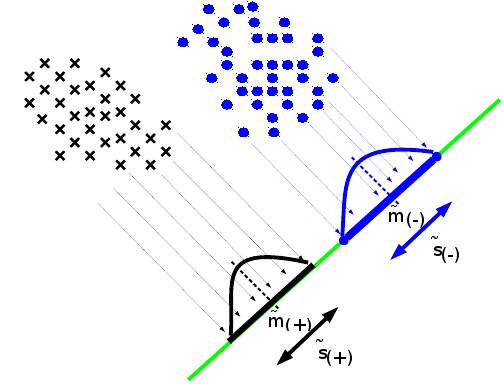
\includegraphics[width=0.5\columnwidth]{Figures/lda}
    \caption{\footnotesize{LDA mapping. The distance $|\tilde{\m}_{(+)}-\tilde{\m}_{(+)}|$} is maximised relative to class variance such as the separability is maximised ($J(\w)$) }
    \label{fig:lda}
\end{figure*}
To express $J(\w)$ in terms of $\w$ and the d-dimensional observed samples, \eqref{eq:lda-class-proj-mean} and \eqref{eq:lda-within-class-scatter} are inserted into \eqref{eq:lda-criteria}, which yields
\begin{equation}
\label{eq:lda-criteria2}
J(\w) = \frac{\w^T \Scat_B \w}{\w^T \Scat_W \w},
\end{equation}
where 
\begin{equation}
\label{lda-b-scatter}
\Scat_B = (\m_{(+)}-\m_{(-)})(\m_{(+)}-\m_{(-)})^T
\end{equation}
is the \emph{between-class scatter matrix}, and 
\begin{equation}
\label{lda-w-scatter}
\Scat_W = \sum_{\x \in \Xc^{(c)}}(\x-\m_{(c)})(\x-\m_{(c)})^T
\end{equation}
is the \emph{within-class scatter matrix}.

Equation \ref{eq:lda-criteria2} is a generalised Rayleigh quotient and can be solved for $\w$ as a generalised eigenvalue problem \citep{duda_pattern_2001}. 

Quadratic Discriminant Analysis (QDA) is a generalisation of LDA to nonlinear boundaries (\textit{i.e.} conic section). 
Unlike LDA, QDA allows different class covariance in the projected space. QDA has also been used for classification of motor imagery tasks \citep{bhattacharyya_performance_2010}. Figure \ref{fig:lda-qda} illustrates the significance of QDA over LDA. 
\begin{figure}[h!]
\centering
\subfigure[]{
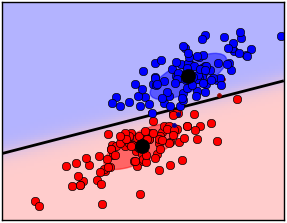
\includegraphics[width=0.4\textwidth]{Figures/lda-separate-data}
\label{fig:lda-separate-data}
}
\subfigure[]{
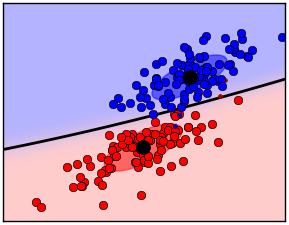
\includegraphics[width=0.4\textwidth]{Figures/qda-separate-data}
\label{fig:qda-separate-data}
}
\subfigure[]{
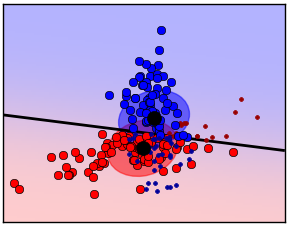
\includegraphics[width=0.4\textwidth]{Figures/lda-overlap-data}
\label{fig:lda-overlap-data}
}
\subfigure[]{
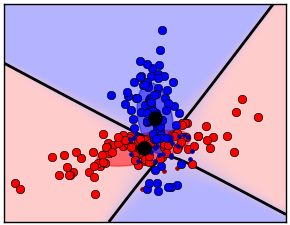
\includegraphics[width=0.4\textwidth]{Figures/qda-overlap-data}
\label{fig:qda-overlap-data}
}
\caption{QDA versus LDA.
Data from two subsets shows with red and blue circles are classified with either LDA (in (a) and (c)) or QDA (in (b) and (d)). The black lines show the classifier separation line. Wrongly classified data are shown with squares instead of circles. 
Class covariances are shown with ellipses of corresponding colours. 
In (a) and (b), the two subsets have similar covariance, while in (c) and (d) they have different covariance \citep{scikit-learn}}
\label{fig:lda-qda}
\end{figure}

%($\x_i \in \Re^d$)

\subsection{SSVEP Processing}% (VEP besed BCI)}
\label{subsec:sign_proc_ssvep}
%CCA + SVM 
Canonical Correlation Analysis (CCA) was recently introduced to classification of SSVEP signal \citep{lin_frequency_2006}. 
It has since been used in the most successful SSVEP-based BCI \citep{bin_online_2009, nakanishi_high-speed_2014}.
It is known that flickering visual stimuli induced an SSVEP that is correlated to the stimuli, \textit{i.e.} the phase and frequency of the signal of interest are known. 
Using this information about the signal of interest, CCA will extract the EEG spatial components that correlate the most with the SSVEP stimuli.
When used as spatial filters, CCA works well when coupled with Support Vector Machine (SVM) classifiers \citep{spuler_one_2012, kalunga_ssvep_2013}.  

\subsubsection{Canonical Correlation Analysis}
\label{subsubsec:cca}
Let  $Y \in \Re^{H \times \dt}$ be a multivariate signal representing the stimulation signal used in recording the EEG signal $\X$.
Per SSVEP principle, $\X$ is expected to be correlated to $Y$. 
Thus CCA will find two projection directions $\w_\X$ and $\w_Y$ such that $\w_X^T \X$ and $\w_Y Y$ have maximal correlation.
$\w_{\X}$ and $\w_Y$ maximises the correlation function $\rho(\w_\X,\w_Y)$:
%In other words, it find the space where the SSVEP -which is correlated to $\Y$, is more observable.
\begin{equation}
\label{eq:cca-rho}
  \begin{split}
    \rho(\w_X,\w_Y) & = \mathrm{corr}(\w_X^T \X,\w_Y Y)
		\\
    & = \frac{\w_{\X}^T \Scat_{\X Y} \w_Y}{\sqrt{\w_{\X}^T \Scat_{\X} \w_X  \w_Y^T \Scat_{Y} \w_Y}},
  \end{split}  
\end{equation}
where $\Scat_{\X Y}$ is the between-set covariance matrix; $\Scat_{\X}$ and $\Scat_{Y}$ are the within-set covariance matrices.
CCA can be solved \citep[as in][]{hardoon_canonical_2004}:
\begin{equation*}
\begin{aligned}
& \underset{\w_X, \w_Y}{\text{maximise}}
& & \w_{\X}^T \Scat_{\X Y} \w_Y \\
& \text{subject to}
& & \w_{\X}^T \Scat_{\X} \w_X = 1, \\
&&& \w_Y^T \Scat_{Y} \w_Y = 1.
\end{aligned}
\end{equation*}
A common way of generating the representation of the simulation signal at frequency $f$ is:
\begin{equation} \label{eq:ref-sig}
    Y_f=\left[
    \begin{array}{c}
    \sin(2\pi f) \\ \cos(2\pi f n) \\
    \vdots \\ \sin(2\pi N_h f n) \\ \cos(2\pi N_h f n)
    \end{array}
    \right],n = \frac{1}{fs}, \frac{2}{fs}, \dots, \frac{\dt}{fs}
\end{equation}  
Where $f_s$ is the EEG sampling frequency, $N_h$ is the number of harmonics, and  $\dt$ the number of sampling points.
$N_h$ is a parameter that can be defined by cross validation.

\subsubsection{Support Vector Machine}
\label{subsubsec:svm}

Support Vector Machines (SVM) have been successfully used in classification of SSVEP signal, and in BCI in general.
The binary SVM decision function is of the form:

\begin{equation}
\label{eq:svm_fct}
y = f(x) = sgn \left( \sum_{i=1}^m y_i \alpha_i k(\x,\x_i) + b \right), y \in \{\pm 1\}
\end{equation}
where $\x$ is the sample variable, $x_i$ a sample in the training data with the label $y_i \in \{\pm 1\}$. $m$ is the number of data samples in the training set, $\alpha_i$ the weight of sample $x_i$ and $b$ an offset.
$k(\cdot,\cdot)$ is a kernel, \textit{i.e.} a function that returns a real number characterising the similarity between its inputs. 
In a Euclidean space, the dot product would often be used as a linear kernel \eqref{eq:linear-kernel}.
Function \eqref{eq:svm_fct} defines a hyperplane of decision boundary that separates samples in the negative class from samples in the positive class.
SVM ignores the influence of training samples $x_i$ that are very far away from the decision boundary by setting their corresponding weight $\alpha_i$ to zero.
Thus, it only relies on a subset of data close to the decision boundary. They are called \emph{Support Vectors}. 
This reduces model complexity and improves generalisation.  
Thought there could possibly exist many hyperplanes that accurately separate data into their specific classes, SVM finds the unique hyperplane that has maximum margin of separation between the support vectors and itself. 
This fact gives SVM classifiers good generalisation performance and robustness to overfitting \citep{scholkopf_learning_2001, ang_filter_2008, ang_filter_2012}. 
To find such a hyperplane SVM solves the following problem:

\begin{equation}
\label{eq:svm_problem}
\begin{aligned}
& \underset{\w \in \dotSpace, b \in \Re}{\text{minimise}}
& & \frac{1}{2} \w^T \w \\
& \text{subject to}
& & y_i( \left\langle \x_i, \w \right\rangle + b )\geq 1, i = 1, \dots, m.
\end{aligned}
\end{equation} 
where $\dotSpace$ is a dot product space, and $m$ is the number of training samples.

\begin{figure}[!h]
\centering
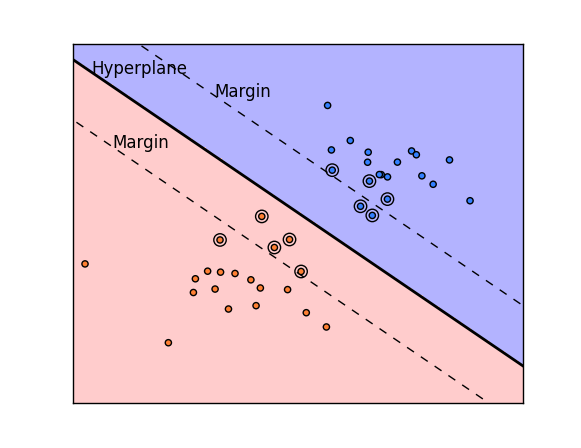
\includegraphics[width=0.8\columnwidth]{Figures/svm}
\caption{Examples of SVM classifiers. 
SVM is applied on 2D artificial data forming two classes represented in red and blue. The hyperplane $\left\langle \x_i, \w \right\rangle + b = 0$ separating the two classes is shown, as well as the margins$\left\langle \x_i, \w \right\rangle + b \geq \frac{1}{||\w||}$. Only few samples relatively close to the hyperplanes are used as support vectors; they are shown with big circles \citep{scikit-learn}.}
\label{fig:svm}
\end{figure}
To achieve nonlinear classification SVM uses kernels other than the dot product.
Such kernels are needed in cases where (1) features are better separated in a higher-dimensional space, (2) features are defined in a space where the dot product is not defined, or (3) the separating line is not linear.
Since SVM is based on the dot product (Eq. \eqref{eq:svm_problem}), the kernel used in the input space $\inputSpace$ corresponds to dot product in $\dotSpace$ via a mapping $\Phi$,

\begin{equation}
\label{eq:kernel-phi}
  \begin{split}
    \Phi : & \inputSpace \rightarrow \dotSpace
		\\
    		   & x \rightarrow \mathbf{\x} := \Phi(x),
  \end{split}  
\end{equation}
such that,
\begin{equation}
\label{eq:kernel-phi2}
k(x,x^{\prime}) = \left\langle \Phi(x), \Phi(x^{\prime}) \right\rangle .
\end{equation}
Examples of such kernels admitting the representation of the form \eqref{eq:kernel-phi} that are often used in SVM are the linear kernel (\textit{i.e.} dot product), the polynomial kernel, and the radial basis function (RBF) kernel.

\begin{figure}[h!]
\centering
\subfigure[]{
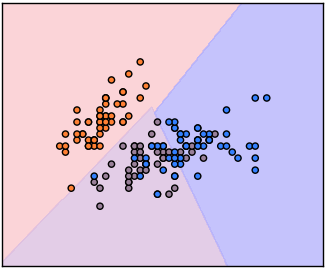
\includegraphics[width=0.3\textwidth]{Figures/svm-linear-kernel}
\label{fig:svm-linear-kernel}
}
\subfigure[]{
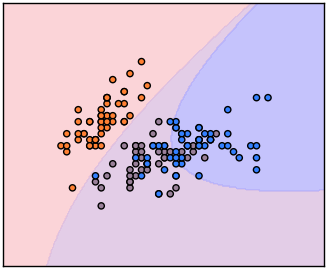
\includegraphics[width=0.3\textwidth]{Figures/svm-poly-kernel}
\label{fig:svm-poly-kernel}
}
\subfigure[]{
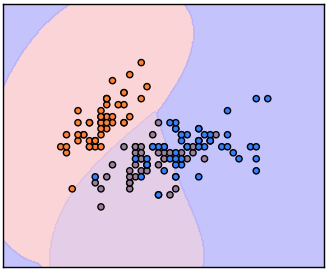
\includegraphics[width=0.3\textwidth]{Figures/svm-rbf-kernel}
\label{fig:svm-rbf-kernel}
}
\caption{Multiclass SVM classification with different kernels on 2D projection of the iris dataset. The decision surface separating three classes are shown. The x-axis and y-axis represent sepal length and sepal width respectively. (a) Linear kernel, (b) polynomial kernel of order 3, (c) RBF kernel \citep{scikit-learn}.}
\label{fig:svm-kernels}
\end{figure}
\emph{Linear kernel}:\\
\begin{equation}
\label{eq:linear-kernel}
k(\x_1,\x_2) = \left\langle \x_1, \x_2 \right\rangle = \x_1^T \x_2.
\end{equation} 
\emph{Polynomial kernels}:\\
\begin{equation}
\label{eq:poly-kernel}
k(x,x^{\prime}) = \left\langle x,x^{\prime} \right\rangle^d, 
\end{equation}
where $d$ is the polynomial degree.\\
\emph{Radial basis function (RBF) kernels}:\\
\begin{equation}
\label{eq:rbf-kernel}
k(x,x^{\prime}) = \exp(- ||x-x^{\prime}||^2), 
\end{equation}
Details on various implementations of SVM classifiers can be found in \citep{chang_libsvm:_2011}

\subsection{P300 Processing}% (ERP-based BCI)}
\label{subsec:sign_proc_p300}

P300 as well as other ERP components are time-locked deflections in the EEG voltage in response to a sensory stimulus.
The time-lock factor is the only known parameter in ERP signals and has been a key factor in their processing. 
Indeed other information about ERP components -- such as phase, amplitude, and period, are either unknown or changing.
They are influenced by concurrent or overlapping components. 

Having a very small amplitude compared to the ongoing brain activity, ERP components are analysed using their occurrence time information.
They are extracted through an averaging of many aligned signal segments of repeated trials. 
After averaging, phenomena that are time-locked to the stimulus will remain while unrelated EEG will cancel out.
This requires that the experiment be repeated a couple of time \citep{rakotomamonjy_ensemble_2005}.

A spatial filter that builds upon the time-locked characteristic of ERP was introduced by \cite{rivet_xdawn_2009} and called xDAWN.
It enhances a specific component in ERP by extracting spatial components that best describe the ERP features reconstructed through averaging of past trials.
It is a major advance in P300-based BCI and ERP analysis in general \citep{rivet_theoretical_2011}. 
Several machine learning competition winners have relied on this approach \citep{barachant_plug&play_2014, barachant_p300-speller:_2015}. 
Using xDAWN, P300 can be processed online with a reduced number of trial repetitions, or even a single trial for ERP identification. 

xDAWN spatial filters can be coupled with any binary classifier used in P300 identification. 
Classification algorithms based on SVM and LDA described in sections \ref{subsec:sign_proc_mi} and \ref{subsec:sign_proc_ssvep} have been particularly used in many successful P300 machine learning \citep{rakotomamonjy_ensemble_2005, krusienski_toward_2008, rivet_xdawn_2009, jrad_sw-svm:_2011, cecotti_robust_2011, mak_optimizing_2011}. 

\subsubsection{xDAWN}  

The first assumption made in xDAWN modelling is that the recorded EEG signal is composed of two typical patterns $P_1$ and $P_2$, one evoked by the ERP stimuli ( $P_1$), and another evoked by any stimulus including ERP stimuli ($P_2$). The second assumption is that the ERP patterns lie in an evoked subspace, hence could be enhanced by a spatial filter.

The first assumption yield the model
\begin{equation}
\X = D_1 P_1 + D_2 P_2 + N,
\end{equation} 
where $D_1 \in \Re^{N_t \times N_1}$ and $D_2 \in \Re^{N_t \times N_2}$ are Toeplitz matrices with first column entries set to one at samples corresponding to ERP stimuli indexes and are zeros otherwise. They define a sort of ERP response temporal distribution in over all recorded EEG samples. $N_1$ and $N_2$ are the number of time samples considered for $P_1$ and $P_2$ respectively. $N$ is the residual noise. 

Based on the second assumption, xDAWN searches for a spatial filter $\xfilt_1^* \in \Re^{N_s}$ that maximises the signal-to-signal-plus-noise ratio (SSNR) $\ssnr(\xfilt)$:
\begin{equation}
\label{eq:xdawn-problem}
\xfilt_1^{*} = \argmax_{\xfilt} \ssnr(\xfilt),
\end{equation}
where the SSNR is estimated with 
\begin{equation}
\label{eq:ssnr}
\hat{\ssnr}(\xfilt) = \frac{\xfilt^T \cov{1} \xfilt}{\xfilt^T \cov{\X} \xfilt}, 
\end{equation} 
where $\cov{1}$ is the estimation of the covariance matrix of the matrix $D_1 P_1$ and  $\cov{\X}$ is the estimation of the covariance matrix of the EEG signal $\X$.
The estimations of covariances are based on estimations of both $P_1$ and $P_2$ \citep[] [as described in ]{rivet_theoretical_2011}.
\\In practice \eqref{eq:ssnr} can be solved for an estimate of the spatial filter $\hat{\xfilt}_1$ with the generalised eigenvalue decomposition (GEVD) of $\cov{1}$ and $\cov{\X}$ to obtain
\begin{equation}
\label{eq:xdawn-gen-eigen}
\cov{1} \hat{\xfilt}_1 = \lambda_1 \cov{\X} \hat{\xfilt}_1,
\end{equation} 
where $\lambda_1$ is the largest eigenvalue returned by the GEVD, and $\hat{\xfilt}_1$ the associated eigenvector. 
\\$P_1$ can be factorised as $P_1 = \mathbf{a}_1 \mathbf{\w}_1^T$ where $\mathbf{a}_1 \in \Re^{N_1}$ is the temporal pattern and $\mathbf{\w}_1 \in \Re^{N_s}$ is its spatial distribution over channels. 
$\mathbf{\w}_1$ is estimated as
\begin{equation}
\hat{\mathbf{\w}}_1 = \cov{\X} \hat{\xfilt}_1.
\end{equation}
 
As a side note, the appellation xDAWN came from the initial method modelling of the EEG signal $X$ obtained in by \cite{rivet_xdawn_2009}:
\begin{equation}
\label{eq:xdawn-initial}
X = D A W^T+N
\end{equation}
where $A$ is the pattern of the synchronised response to the ERP stimulus, $D$ is the Toeplitz matrix defining the samples of the EEG epoch where the pattern of the synchronised response are active (like a temporal distribution), $W$ is the spatial distribution of the ERP over channels, and N is the ongoing EEG.    
%\subsection{Other Machine learning methods}
%\label{subsec:sign_proc_other}

%- Mention other methods used in BCI and references to articles where they were used.
%		e.g. ANN, ICA, PCA
%- Riemmanian approach MDM

\subsection{Discussion}

There is a variety of machine learning techniques that have been explored for classification in brain-computer interfaces \citep{lotte_review_2007, nicolas-alonso_brain_2012, bashashati_survey_2007, khorshidtalab_eeg_2011, krusienski_critical_2011}.  
The ones described in this section are among the most successful and have thus been used recurrently in BCI research.
While the design or the choice of spatial filters is guided by the neurological phenomenon used in a particular BCI type, the classification is achieved using standard classifiers that best separate the extracted features. 
Thus classifiers can be used interchangeably over various BCI types.  

A remarkable fact about the discussed methods is that they all involve in a way or another, an estimate of covariance matrices or scatter matrices.
Indeed, covariance matrices and scatter matrices capture a great deal of information about the signal of interest in the EEG. 
They contain information such as spatial patterns of neuronal activities involves in mental tasks, data distribution, and data variance, which are all crucial for the classification task.
It is also noticed that nearly all algorithms -- with the exception of kernel SVM — are developed from vector space or Euclidean space point of view. 
As has been said in chapter \ref{chap:intro}, and will be discussed in detail in chapter \ref{chap:riem-geom-bci}, covariance matrices lie on a curved space where Euclidean geometry is not suitable \citep{congedo_new_2013}.

BCI learning algorithms often face the \emph{curse of dimensionality}, a phenomenon that describes the relationship between the sample size (\textit{i.e.} number of observations in training set) and dimensionality (\textit{i.e.} dimension of feature space): the amount of data needed to achieve sound statistical learning grows exponentially with the dimensionality \citep{fukunaga_introduction_1990, foley_considerations_1972, kanal_dimensionality_1971, raudys_small_1991}. 
If the sample size to dimensionality ratio is not large enough, the algorithms will be strongly biased.
Although this is a general problem in machine learning, it is particularly present is EEG-based BCI, where a single observation is described by many features (e.g. time samples, frequency bands) from multiple sources.
Such a big feature space would require very large training samples which are not usually attainable.
The samples are recoded through thorough experiment protocols that can be conducted only for a relatively short period of time.
A common way of alleviating the curse of dimensionality is through feature selection and dimensionality reduction techniques such as PCA and ICA. 

A small training set may also lead to the problem of \emph{overfitting}. 
When the training set is too small to represent the entire population, the model trained on such data will describe a separating line that is dependent on processes specific to the observed data rather than the global underlying discriminating factors \citep{hill_classifying_2006}.
This also happens when the model is overtrained or too complex for the task at hand. 
The fact that both spatial filter and classifier parameters are learned from the same training sample increases the risks of overfitting.
In machine learning when the training set is deemed too small (or non-existent) to train a statistical model, notions of \emph{domain adaptation} and \emph{transfer learning} are used \citep{pan_survey_2010}. 
In domain adaptation, exiting data drawn from a different distribution are adapted and used to train a task on data from another distribution. 
In transfer learning, knowledge learned from previous data is used to lighten the learning process and alleviate the lack of training data.
These two options are  being investigated in machine learning for BCI \citep{kang_composite_2009, wang_review_2015}.    

 
%Une conclusion contenant les conclusin de toutes les section ?
%-------------------------------------------------------------------------

%%% #############################################################################################################################
\comment{
% THIS PART WILL BE IN THE RIEMANNIAN GEOMETRY CHAPTER
%\subsection{Riemannian geometry based algorithms}
%\label{subsec:sign_proc_riemann}
%\note{Introduce Riemannian space, and Riemannian geometry. Explain why it is different from Euclidean geometry.
%Show graphically the geometry of SPD matrices. And mention the fact that Covariance matrices have been treated in Euclidean space. And mention the work of congedo and Barachant's team and the ones mentioned in Congedo HDR as being the first considering the geometry of covariance matrices in EEG. N.B. The review will be kept for the chapter on online classif.}\\

Information geometry provides useful tools for various machine learning and optimisation problems. 
In machine learning, Symmetric Positive-Definite (SPD) matrices % and probability distribution functions (pdf)
 have been used in various applications where features and data  are only considered in the Euclidean space. % were explored with tools from Riemannian geometry.
Indeed, covariance matrices lie in the space of SPD matrices which is a subset of the Euclidean space when considered with the scalar product.
But the same space of SPD matrices, endowed with a differential structure, induces a Riemannian manifold.
%Probability distribution functions of observed data and their covariance matrices, which are SPD, are elements of a Riemannian manifold. %zz: j'ai chang? le paragraphe car il parlait de riemannian structure, je ne suis pas sur de la d?finition d'une structure riemannienne. Est ce que tu pourrais m'indiquer o? tu as lu ?a ?

% *La geom?trie riemannienne pour am?liorer les algorithmes des machine learning existant

%To overcome the inadequacy of applying algorithms and operations defined in Euclidian space on data lying on Riemannian manifolds, %zz:idem pour les structure

%Use of kernels to use algo developed for Euclidean space
Riemannian geometry can improve machine learning algorithms, taking into consideration the underlying structure of the considered space explicitly.
%Riemannian geometry have been used to improve machine learning algorithms, most of which were mainly developed for data in euclidean space, to apply them on data lying on Riemannian manifold.  
Three kinds of approaches in the literature use the data geometry in machine learning. 
The first one relies on the mapping of the Riemannian manifold onto a Euclidean vector space. % where Euclidean geometry applies.
One such mapping, called logarithmic mapping, exists between the manifold and its tangent space, which is a Euclidean space, and has been used in classification tasks for BCI~\citep{barachant2012bci,BAR13}. 
%The Riemannian Log map induces a direct mapping on the tangent space, those tangent spaces are Euclidean.
%Mapping on the tangent space using the Riemannian Log map \cite{barachant2012bci} could be used as tangent spaces on Riemannian manifold are known to be Euclidean. 
Other kernels have been applied successfully to this end: Stein kernel, Log-Euclidean kernels as well as their normalised versions~\citep{yger2013review}.
The main idea is to map the input data to a high-dimensional feature space, providing a rich and hopefully linearly separable representation.
The so-called kernel trick is to provide a kernel function, which computes an inner product in the feature space directly from points lying in the input space, defining a Reproducing Kernel Hilbert Space (RKHS).
The family of kernels defined on the Riemannian manifold allows implementing extension of all kernel-based methods, such as SVM, kernel-PCA or kernel $k$-means~\citep{jayasumana2013kernel}.
%Using kernels that are symmetric positive definite and adapted from Euclidean metrics to the Riemannian geodesic metrics to map SPD matrices to higher dimension linear Hilbert space works well on kernel-based algorithms such as SVM and kernel PCA applied to data on Riemannian manifold
Apart from the kernel approaches, once the data are mapped onto a vector space, any machine learning algorithm working in Euclidean space, such as LDA, could be applied~\citep{barachant2012multiclass}.

% Reformulation and adaptation of algorithmes supervis?s :
A second kind of machine learning approach exploit the underlying geometry of the data.
Instead of mapping the data to a Euclidean space, either a tangent space or an RKHS, the algorithms are adapted to Riemannian space. 
% Using kernels makes the numerous existing machine learning algorithms readily usable for data originally on Riemannian manifold. However, some features might be squeezed out during the mapping process. 
% Another avenue has been explored, where the data are left in their original Riemannian space, whereas the algorithms initially developed for Euclidean space are adapted to Riemannian space.
For instance, sparse coding algorithm has been adapted to Riemannian manifold, using the geodesic distance to estimate the data point and its sparse estimate~\citep{xie2013nonlinear}.
%When data points and atoms used to generate them belong to a Riemannian space $\Ma$, they do no support vector space structure. Hence data points are not estimated as linear combination of atoms (as it is the case in sparse coding), rather with a nonlinear sparse coding; and the error (distance) between the data point and its estimate from sparse coding is a geodesic \cite{xie2013nonlinear}.
Similarly nonlinear dimensionality reduction techniques have been adapted to Riemannian manifold, such as Laplacian Eigenmaps (LE), Locally Linear Embedding (LLE), and Hessian LLE. 
This adaptation was used to cluster data using their pdfs \citep{goh2008unsupervised} or covariance matrices \citep{goh2008clustering} as features. 
Another example is the adaptation of interpolation and filtering of data to Riemannian space performed in \citep{PEN06}, where an affine-invariant Riemannian metric is also proposed to offer a geodesically complete manifold i.e a manifold with no edge and no singular point that can be reached in a finite time.  
%The authors of these techniques assume that the data features belonging to $\Ma$ are distributed in submanifolds of $\Ma$; and hence each of the submanifold will be mapped to a different point in $\Re^n$. % zz: the notation
%\textit{k}-disconnected union of \textit{m} \textit{k}-connected submanifolds of $\Ma$; and hence each of the submanifold will be mapped to a different point in $\Re^m$. % zz: the notation

  
% * les outils qui travaillent directement dans l'espace des vari?t?s riemaniennes : (Newly developed algo for features riemanian manifold)
In the last kind of approach, instead of adapting existing algorithms from Euclidean to Riemannian geometry, new algorithms are developed directly for Riemannian manifolds.
% MDRM
The \emph{minimum distance to Riemannian mean} (MDRM) relies on a Riemannian metric to implement a multi-class classifier and have been applied on EEG.
%an equivalent of $k$-mean in % between covariance matrices of EEG to classify trials from multiclass motor imagery BCI.
New EEG trials are assigned to the class whose average covariance matrix is the closest to the trial covariance matrix~\citep{barachant2012multiclass}.
The MDRM classification can be preceded by a filtering of covariance matrices, like in~\citep{barachant2010riemannian} where covariance matrices are filtered with LDA component in the tangent space, then brought back to the Riemannian space for classification with MDRM. 
Another example is the \emph{Riemannian Potato} \citep{barachant2013riemannian}, an unsupervised and adaptive artifact detection method, providing an online adaptive EEG filtering (\textit{i.e.} outlier removal). 
Incoming signals are rejected if their covariance matrix lies beyond a predefined distance z-score from the mean covariance matrix, computed from a sliding window.
% which is defined adaptively along signal recording. 
With the same objective of achieving robustness to noise that affect covariance matrices, Riemannian geometry is used to solve divergence functions of pdfs~\citep{amari2010information}.
This allows to reformulate the CSP as the maximisation of the divergence between the distributions of data from two different classes corresponding to two cognitive states~\citep{samek2013robust, samek2014information}. 
Using the \emph{\beta divergence} the obtained CSP is robust to outliers in sample covariance matrices and this algorithm is successfully applied to the EEG filtering for BCI.   
Riemannian metrics are also used for the EEG channel selection~\citep{barachant2011channel} and the selection of the most discriminatory spatial filters in CSP~\citep{barachant2010common}.  

%%Feature (filters) selection in CSP
%In \cite{barachant2010common}, Riemannian distance is used to select the most discriminatory spatial filters in CSP from eigenvectors of the sum of class mean covariance matrices -- which are obtained with a Riemannian mean. 
%It is established that each eigenvalue corresponding to each filter (eigenvector) contribute to the Riemannian distance between the class mean covariance matrices. 
%Filters whose eigenvalue contribute the most are selected.
%%channel selection
%In \cite{barachant2011channel}, the authors propose a channel selection technique using backward elimination principle. 
%Channels that maximize the Riemannian distance between Riemannian mean covariance matrices of different classes are kept. 

%Riemannian Geometry for Evoked potential and ERP

Applications of Riemannian geometry to BCI mentioned thus far are focusing on motor imagery (MI) paradigm.
%In MI experiment, the subject is asked to imagine a movement (usually hand, feet or tongue), generating Event-Related Synchronization and Desynchronization (ERD/ERS) in pre-motor brain area.
Riemannian BCI is well suited for MI experiments as the spatial information linked with synchronisation is directly embedded in covariance matrices obtained from multichannel recordings.
%needed to identify regions of synchronization and regions of desynchronization is well embedded in covariance matrices obtained from the multichannel observed data.
However, for BCI that rely on Evoked Potential such as SSVEP or Event Related Potential (ERP), as P300, both frequential and temporal information are needed; the spatial covariance matrix does not contain this information. 
%-By an extended definition od SCM
To apply Riemannian geometry to SSVEP and ERP, the sample covariance matrices can be defined from a rearrangement of the recorded data. 
The rearrangement is done such that the temporal or frequency information is captured~\citep{congedo2013new}. 
%-By new definition of riemannian distance
With similar motivations, \cite{li2009eeg} and \cite{li2012electroencephalogram} defined a new Riemannian distance between SPD matrices that would take into account a weighting factor on matrices. 
They use this new distance as a dissimilarity between weighted matrices of power spectral density to classify EEG into different sleep state by $k$-nearest neighbours. 
%Matrices of power spectral density are function of the frequency band $\omega$, and within each EEG epoch varying $\omega$ results in a curve on the manifold. the proposed metric measures the distance between such curves.
}




%\section{New BCI approaches}%Hybrides, Passive, and Neurofeedback
%\label{sec: }

\section{Riemannian Approaches in Machine Learning}
\label{sec:riemann_approach}

%\note{Introduce Riemannian space, and riemannian geomtry. Explain why it is different from Euclidean geometry.
%Show graphically the geometry of SPD matrices. And mention the fact that Covariance matrices have been treated in EUclidean space. And mention the work of congedo and Barachant's team and the ones mentioned in Congedo HDR as being the first considering the geometry of covariance matrices in EEG. N.B. The review will be kept for the chapter on online classif.}\\


%Consequently, spatial filtering methods have been developed or adapted. 
%Most of them (\textit{i.e.} Common Spatial Patern (CSP), xDAWN, and Canonical Correlation Analysis (CCA)) are based on covariance matrix estimations. 
%Covariance matrices are key in the representation of information contained in EEG signal and constitute an important feature in their classification.
%In most of the existing machine learning algorithms, covariance matrices are treated as elements of the Euclidean space. 
%However, being Symmetric and Positive-Definite (SPD), covariance matrices lie on a curved space that is identified as a Riemannian manifold. 
%Using covariance matrices as features for classification of EEG signals and handling them with the tools provided by Riemannian geometry provide a robust framework for EEG representation and learning. 


Information geometry provides useful tools for various machine learning and optimisation problems. 
In machine learning, Symmetric Definite-Positive (SPD)	 matrices % and probability distribution functions (pdf)
 have been used in various applications where features and data  are only considered in the Euclidean space. % were explored with tools from Riemannian geometry.
A typical case where SPD could be found in machine learning is in covariance matrices which are of paramount importance in feature representation (Section \ref{sec:sig_process}).
The covariance matrices are constrained to a special topology by their properties namely symmetry, positive definiteness, strict positivity of the diagonal elements, and the Cauchy-Schwarz inequalities (further discussed in Section \ref{subsec:mean}).
Indeed, covariance matrices lie in the space of SPD matrices which is a subset of the Euclidean space when considered with the scalar product.
But the same space of SPD matrices, endowed with a differential structure, induces a Riemannian manifold.

Riemannian geometry can improve machine learning algorithms, taking into consideration the underlying structure of the considered space explicitly.
%Riemannian geometry have been used to improve machine learning algorithms, most of which were mainly developed for data in euclidean space, to apply them on data lying on Riemannian manifold.  
Three kinds of approaches in the literature use the data geometry in machine learning. 
The first one relies on the mapping of the Riemannian manifold onto a Euclidean vector space. % where Euclidean geometry applies.
One such mapping, called logarithmic mapping, exists between the manifold and its tangent space, which is a Euclidean space, and has been used in classification tasks for BCI \citep{barachant_bci_2012,barachant_classification_2013}. 
%The Riemannian Log map induces a direct mapping on the tangent space, those tangent spaces are Euclidean.
%Mapping on the tangent space using the Riemannian Log map \cite{barachant2012bci} could be used as tangent spaces on Riemannian manifold are known to be Euclidean. 
Other kernels have been applied successfully to this end: Stein kernel, Log-Euclidean kernels as well as their normalised versions \citep{yger_review_2013}.
The main idea is to map the input data to a high-dimensional feature space, providing a rich and hopefully linearly separable representation.
The so-called kernel trick is to provide a kernel function, which computes an inner product in the feature space directly from points lying in the input space, defining a Reproducing Kernel Hilbert Space (RKHS).
The family of kernels defined on the Riemannian manifold allows implementing extension of all kernel-based methods, such as SVM, kernel-PCA or kernel $k$-means \citep{jayasumana_kernel_2013}.
%Using kernels that are symmetric positive definite and adapted from Euclidean metrics to the Riemannian geodesic metrics to map SPD matrices to higher dimension linear Hilbert space works well on kernel-based algorithms such as SVM and kernel PCA applied to data on Riemannian manifold
Apart from the kernel approaches, once the data are mapped onto a vector space, any machine learning algorithm working in Euclidean space, such as LDA, could be applied \citep{barachant_multiclass_2012}.

% Reformulation and adaptation of algorithmes supervis?s :
A second kind of machine learning approach exploit the underlying geometry of the data.
Instead of mapping the data to a Euclidean space, either a tangent space or an RKHS, the algorithms are adapted to Riemannian space. 
% Using kernels makes the numerous existing machine learning algorithms readily usable for data originally on Riemannian manifold. However, some features might be squeezed out during the mapping process. 
% Another avenue has been explored, where the data are left in their original Riemannian space, whereas the algorithms initially developed for Euclidean space are adapted to Riemannian space.
For instance, sparse coding algorithm has been adapted to Riemannian manifold, using the geodesic distance to estimate the data point and its sparse estimate \citep{xie_nonlinear_2013}.
%When data points and atoms used to generate them belong to a Riemannian space $\Ma$, they do no support vector space structure. Hence data points are not estimated as linear combination of atoms (as it is the case in sparse coding), rather with a nonlinear sparse coding; and the error (distance) between the data point and its estimate from sparse coding is a geodesic \cite{xie2013nonlinear}.
Similarly nonlinear dimensionality reduction techniques have been adapted to Riemannian manifold, such as Laplacian Eigenmaps (LE), Locally Linear Embedding (LLE), and Hessian LLE. 
This adaptation was used to cluster data using their pdfs \citep{goh_unsupervised_2008} or covariance matrices \citep{goh_clustering_2008} as a feature. 
Another example is the adaptation of interpolation and filtering of data to Riemannian space performed in \citep{pennec_riemannian_2006}, where an affine-invariant Riemannian metric is also proposed to offer a geodesically complete manifold \textit{i.e.} a manifold with no edge and no singular point that can be reached in a finite time.  
%The authors of these techniques assume that the data features belonging to $\Ma$ are distributed in submanifolds of $\Ma$; and hence each of the submanifold will be mapped to a different point in $\Re^n$. % zz: the notation
%\textit{k}-disconnected union of \textit{m} \textit{k}-connected submanifolds of $\Ma$; and hence each of the submanifold will be mapped to a different point in $\Re^m$. % zz: the notation

  
% * les outils qui travaillent directement dans l'espace des vari?t?s riemaniennes : (Newly developed algo for features riemanian manifold)
In the last kind of approach, instead of adapting existing algorithms from Euclidean to Riemannian geometry, new algorithms are developed directly for Riemannian manifolds.
% MDRM
The \emph{minimum distance to Riemannian mean} (MDRM) relies on a Riemannian metric to implement a multi-class classifier and have been applied on EEG.
%an equivalent of $k$-mean in % between covariance matrices of EEG to classify trials from multiclass motor imagery BCI.
New EEG trials are assigned to the class whose average covariance matrix is the closest to the trial covariance matrix \citep{barachant_multiclass_2012}.
The MDRM classification can be preceded by a filtering of covariance matrices, like in \citep{barachant_riemannian_2010} where covariance matrices are filtered with LDA component in the tangent space, then brought back to the Riemannian space for classification with MDRM. 
Another example is the \emph{Riemannian Potato} \citep{barachant_riemannian_2013}, an unsupervised and adaptive artifact detection method, providing an online adaptive EEG filtering (i.e outlier removal). 
Incoming signals are rejected if their covariance matrix lies beyond a predefined distance z-score from the mean covariance matrix, computed from a sliding window.
% which is defined adaptively along signal recording. 
With the same objective of achieving robustness to noise that affect covariance matrices, Riemannian geometry is used to solve divergence functions of pdfs \citep{amari_information_2010}.
This allows to reformulate the CSP as the maximisation of the divergence between the distributions of data from two different classes corresponding to two cognitive states \citep{samek_robust_2013,samek_information_2014}. 
Using the \emph{beta divergence} the obtained CSP is robust to outliers in sample covariance matrices and this algorithm is successfully applied to the EEG filtering for BCI.   
Riemannian metrics are also used for the EEG channel selection \citep{barachant_channel_2011} and the selection of the most discriminatory spatial filters in CSP \citep{barachant_common_2010}.  

%%Feature (filters) selection in CSP
%In \cite{barachant2010common}, Riemannian distance is used to select the most discriminatory spatial filters in CSP from eigenvectors of the sum of class mean covariance matrices -- which are obtained with a Riemannian mean. 
%It is established that each eigenvalue corresponding to each filter (eigenvector) contribute to the Riemannian distance between the class mean covariance matrices. 
%Filters whose eigenvalue contribute the most are selected.
%%channel selection
%In \cite{barachant2011channel}, the authors propose a channel selection technique using backward elimination principle. 
%Channels that maximize the Riemannian distance between Riemannian mean covariance matrices of different classes are kept. 

%Riemannian Geometry for Evoked potential and ERP

Applications of Riemannian geometry to BCI mentioned thus far are focusing on motor imagery (MI) paradigm.
In MI experiments, the subject is asked to imagine a movement (usually hand, feet or tongue), generating Event-Related Synchronisation and Desynchronisation (ERD/ERS) in pre-motor brain area.
Riemannian BCI is well suited for MI experiments as the spatial information linked with synchronisation is directly embedded in covariance matrices obtained from multichannel recordings.
%needed to identify regions of synchronization and regions of desynchronization is well embedded in covariance matrices obtained from the multichannel observed data.
However, for BCI that rely on Evoked Potential such as SSVEP or Event Related Potential (ERP), as P300, both frequential and temporal information are needed; the spatial covariance matrix does not contain this information. 
%-By an extended definition od SCM
To apply Riemannian geometry to SSVEP and ERP, the sample covariance matrices can be defined from a rearrangement of the recorded data. 
The rearrangement is done such that the temporal or frequency information is captured \citep{congedo_new_2013}. 
%-By new definition of riemannian distance
With similar motivations, \cite{li_eeg_2009, li_electroencephalogram_2012} defined a new Riemannian distance between SPD matrices that would take into account a weighting factor on matrices. 
They use this new distance as a dissimilarity between weighted matrices of power spectral density to classify EEG into different sleep state by $k$-nearest neighbours. 
%Matrices of power spectral density are function of the frequency band $\omega$, and within each EEG epoch varying $\omega$ results in a curve on the manifold. the proposed metric measures the distance between such curves.

\section{New Trend in BCI Systems}
\label{sec:new_trends_BCI}
From the current state-of-the-art in BCI for control and communication (Chapter \ref{chap:lit_survey_neuro}), it has become clear that the limitations in this field are such that BCI cannot replace traditional input modalities for human machine interface, nor match their performance.
This restrains the use of BCI to a population with limited residual muscular ability to use traditional input devices.

Recently, research has been exploring ways of extending the use of BCI to a larger population -- including healthy subject, in applications that will suffer less from BCI limitations such as the limited bandwidth (low information transfer rate), the BCI illiteracy, the training required to intentionally alter or generate patterns of brain signals, as well as the cognitive workload involved in performing the BCI tasks. 
This effort has resulted in applications (or modalities) that tend to move away from fully relying on BCI as the sole input modality for human machine interfaces.
The prominent examples in this trend are \emph{hybrid brain-computer interfaces} (hBCI) \citep{millan_combining_2010} and \emph{passive brain-computer interfaces} (pBCI) \citep{zander_towards_2011}.
In the following lines both of them are further discussed. %, hBCI first, then pBCI.

\subsection{Hybrid BCI systems}
\label{sec:hBCI-systems}

One way of alleviating limitations in BCI is to combine multiple modalities or neurological phenomena. This has the potential of achieving higher information transfer rate and increasing degree of freedom. 
It is also a way to compensate a weakness in a particular type of brain-computer interface by relying on another one.
Many combinations are possible: SSVEP and motor imagery, P300 and error related potential, etc. 
This has been suggested as a solution to BCI illiteracy as a subject who is illiterate toward a particular BCI type, e.g. SSVEP, might show efficiency in using another BCI type e.g. motor imagery.

The existing hBCI can be categorised according to (1) the type of %activities or 
signals combined and (2) how the signals %the manner the activities or signals
are combined to achieve the desired task.
According to the type of %activities or 
signal used, two types of hBCI are distinguished. 
In the first type, different brain signals (e.g. motor imagery, evoked potentials) are combined \citep{ferrez_simultaneous_2008, allison_toward_2010, finke_hybrid_2011}, while in the second a brain signal is combined with other biosignals e.g. ECG \citep{scherer_self-initiation_2007} or EMG \citep{leeb_multimodal_2010}. 
The hBCI combining EMG and a brain signal is the only case where the residual muscular functionalities of the patients are used.
%The hBCI combined EMG and a brain signal is the only case where the 
%The residual muscular functionality are only considered in the case of EMG residual muscular functionality of the patients used. 
%Only in the case of combining brain activities and EMG is the residual muscular functionality of the patients used. 
Apart from this approach, residual muscular functionalities have been combined with BCI in a neuroprosthesis where the patient uses arm movement for reaching positions and BCI for grasping objects \citep{millan_asynchronous_2009, millan_noninvasive_2004}. 
Though in this approach BCI is used as an additional channel to assistive technologies, using residual muscular functionality, BCI literature refers to it also as hBCI \citep{millan_combining_2010}.

Depending on the combination of interfaces (or control channel), several control strategies are possible.
The first one is to assign one specific task per interface.
%According to the manner in which the activities or signals (\textit{i.e.} control channels) are combined, they can operate different components of the assistive device or different tasks.
Another possibility is to merge all interfaces in a weighted combination to achieve a unique task with higher accuracy.
Finally, they can be used alternatively so as to allow users to smoothly switch from one interface to another depending on their performance or preference. 
The work of \cite{millan_combining_2010} provides a comprehensive review of the existing hBCI approaches and their applications.
  
%\textcolor{red}{To extend.}
\subsection{Passive BCI}

%* Definition + History
While BCI relies on brain activities intentionally controlled by the user, there is a lot more information related to the user's states not intentionally expressed, that can be obtained from a real-time brain signal decoding (RBSD) and used in human computer/machine interaction (HCI or HMI).
For decades, RBSD has been used for cognitive monitoring providing a way of looking into one's cognitive and affective states \citep{zander_towards_2011}.
Passive BCI uses this implicit information as an additional input modality in HCI.    
%* Objectives (motivation) + problem solved from BCI
%	- Target popo
%	- bandwidth, etc. axtension to any HCI
Thus, the objective of BCI is moved from control and communication to improving HCI by using brain information not intentionally generated by the user. 
This opens BCI to all HCI applications and to a larger population.

In BCI for communication and control, the brain activities are consciously generated by the user either directly or indirectly resulting in a considerable cognitive workload which is not present in pBCI.
\cite{zander_towards_2011} categorises BCI in active, reactive, and passive. 
Active BCI and reactive BCI are used for control and communication. 
In the first, the brain patterns are directly and consciously controlled by the user (e.g. motor imagery). 
In the second, they are indirectly generated with the help of external stimulus (e.g. SSVEP).

pBCI does not require training users to generate specific patterns in brain signals, and thus not affected by problems of BCI illiteracy and heavy cognitive workload.
Moreover pBCI does not suffer from the bandwidth limitation as it is used on top of other HCI input modalities. 
%* Few info about the technique: Basically uses all components of BCI with few changes.
%		- Signal used: EEG and fNIRS
%		- Information sought after	
%		- Brain pattern and signal features
%pBCI uses the same technology developed for active BCI.
%EEG and fNIRS are preferred mainly for their portability as the BCI is to be used in tandem with other HCI input modalities [ref: Girouard-designing-2013].
pBCI uses various brain signal features to infer information about the cognitive and affective state of the user \citep{george_overview_2010}.   
%* Applications of pBCI
%	- Gaming, etc (may be grouped under adaptive context: adaptation of environment) 
%	- adapting control (automation, safety driving, etc.)
%	- error correction
%	- Multimedia tagging
%	- epilepsy
%	- Musical
%	- Neurofeedback: - training, emotion regulation, etc
Using this information, pBCI has been deployed in many HCI applications.
% with promising result as it improves the interaction between man and computer. 
In gaming for instance, pBCI has been used to adapt the game interface and difficulty level to the affective and cognitive state of the player. 
This has crucial importance as the whole point of recreational activities such as games themselves is to relax, engage and entertain the user. 
With pBCI it is possible to measure this information and adapt while the user is still playing to ensure a balance between frustration, rewards, pleasure, etc. for overall satisfaction \citep{cutrell_bci_2008,girouard_designing_2013}.

Similarly, pBCI can be used for adaptive control in delicate applications such as aeroplane piloting, driving semi-autonomous cars, and automated industries. 
As control can be shared between man and machine, pBCI can detect when man control is likely to be defective--due to stress, fatigue, somnolence, etc., and allow the machine to take over \citep{cutrell_bci_2008,george_overview_2010}. 

pBCI can also be used to detect and correct errors in HCI. When a user notices an erroneous response of a machine, an error related potential is evoked in their brain, and can be used in pBCI to correct the error. Errors are very common in active BCI and are more machine-made than human-made. With pBCI, BCI systems can fix their own mistakes \citep{ferrez_error-related_2008, ferrez_simultaneous_2008,george_overview_2010}.

pBCI is not only limited to human-machine interactions. Other applications include prevention of epileptic seizures \citep{liang_closed-loop_2010}, neurofeedback \citep{huster_braincomputer_2014,hao_visual_2014}, and music creation \citep{yuksel_implicit_2015}, etc.

%* pBCI versus cognitive monitoring
%Note that pBCI is not a mere cognitive monitoring; implicit information obtained from RBSB should be used in the HCI.			


\section{Proposed Approach}
\label{sec:proposed-approach}

To address BCI problems raised in Section \ref{sec:research_problem}, namely user specificity, robustness of EEG representation and learning, and sufficiency of training data, two main avenues are explored: a hybrid BCI approach and a machine learning approach based on Riemannian geometry.
The first aims at giving a solution to the problem of BCI users' specificity while the second tackles problems of EEG representation and data sufficiency.  

\subsection*{A Hybrid BCI Approach}
The hybrid approach taken in this work combines brain signals (cerebral commands) with haptic command from user's residual motor skills.
This approach offloads or takes a part of the control away from BCI by allowing the use of residual motor skills.
The cerebral command limited by BCI state-of-the-art and the haptic command limited by user residual abilities complement each other.
It has the advantage of reactive BCI systems; they only require the user to be attentive to the external stimuli; the pattern generated are merely a natural brain response. Thus, less training requires from the user, and lower cognitive workload involved.
A touchless interface is used as the input modality for haptic commands. It is designed for a comfortable 3-D navigation, particularly for users with limited hand control. 

The concept of hybrid BCI has been known mostly as a combination of various neurological phenomenon, combining various BCI types in one system. In the largest sense, hybrid BCI has combined brain signals and other biosignals \citep{millan_combining_2010}. 
In this work, the concept of hybrid BCI is stretched further  to include muscular commands. 
A SSVEP based BCI is used for the cerebral command. 

\subsection*{Machine Learning with Riemannian Framework}
The proposed approach uses covariance matrices of EEG signals in a Riemannian framework.
The covariance matrices are key in the representation of information contained in the EEG signal and constitute an important feature in their classification. 
They are handled with tools provided by the Riemannian geometry to alleviate difficulties in current BCI machine learning.
Using covariance matrices as features, the machine learning pipeline depicted in Figure \ref{fig:porposed-pipeline} is adopted.
It consists of three main phases: offline model selection, training phase, and classification.
Unlike the one in Figure \ref{fig:processing_pipeline}, it does not include a spatial filtering phase.

\begin{figure}
\centering
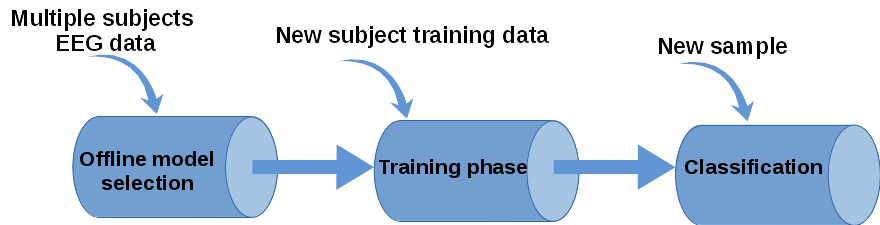
\includegraphics[width=0.8\columnwidth]{Figures/proposed-processing-pipeline.png}
\caption{Adopted machine learning pipeline. It consists of 3 main phases: 1) Offline model selection: A number of preprocessing and classifiers are tested on a collection of data from multiple subjects, the best combination is selected. 2) Training phase: Classifier parameters are trained for each new subject before classification. 3) Classification: A new [unseen] sample is preprocessed similarly to training data, then classified.}
\label{fig:porposed-pipeline}
\end{figure}  
% ------------------------------------------------------------------------
% -*-TeX-*- -*-Hard-*- Smart Wrapping
% ------------------------------------------------------------------------
%%% Literature Survey --------------------------------------------------

%\addtolength{\topmargin}{-.875in}
%\addtolength{\textheight}{.875in}
%\footskip
%\nonumchapter{Literature Survey}
\chapter{Hybrid Brain-Computer Interface}
\label{chap:hBCI}
\epigraph{Anybody who has been seriously engaged in scientific work of any kind realises that over the entrance to the gates of the temple of science are written the words: Ye must have faith. It is a quality which the scientist cannot dispense with.}{--- \textup{Max Planck}}
%-------------------------------------------------------------------------

\section{Introduction}%Hybrides, Passive, and Neurofeedback
\label{sec:hBCI-intro}

% In rehabilition, one must find a solution which could be adapted to the need and the capacities of each user, because each person is unique.
% people with disability often have residual motor capabilities and want to use it. BCI only system are not robust enough and contradict with the subject's desire to use the working part of their body. A hybrid approach allows the user to combined his residual skills with the possbility of using a BCI to alleviate some boring/repetitive task.
% Claim : We propose a new methodology for disabled people, using an hybrid approach where a physical interface is complemented by a brain computer interface.
% Contribution: Our contribution are threefold : we define a new methodology for design control system for disabled people, we introduce a new learning scheme for BCI and we propose an implementation of  the whole system for two applications in rehabilitation robotics.

Rehabilitation and assistive technologies aim at developing solutions \emph{adapted} to the subjects' disabilities.
A crucial aspect is to take into account the specificities of each person and to propose technical solutions which make use of their residual motor capabilities.
As a simple example, an electric wheelchair will not interest someone who has still some strength in his upper limbs but the same person could be interested by the assistance of an electric motor for driving a manual wheelchair. 
% The aim in rehabilitation and assistive technology is to develop solutions that are adequate to patients' disabilities. 
% Rather than the patients being obliged to adapt to the assistive technologies regardless of their conditions, the approach in rehabilitation is for the assistive technology devices to adapt to the needs of patients, taking into account their disabilities while allowing them to use their residual motor capabilities. 
%Hence in this work, we propose a new methodology for disabled people, using an hybrid approach where a physical interface is complemented by a Brain-Computer Interface (BCI). 

%BCI do not rely on subjects' residual motor capabilities but current system have shown limited performances.
%To overcome these limitations, we design a system that allows the users to use both their brain signals and their residual motor abilities for control tasks.
%Our contribution are threefold : we define a new methodology for a hybrid control system, we introduce a new learning scheme for SSVEP-based BCI and we propose an implementation of  the whole system in two applications of rehabilitation robotics. 

BCI, in their essence, overlook the muscular system. 
They do not rely on subjects' residual motor capabilities. But because of the limited performances of current BCI systems, patients might desire to use their residual motor abilities. 
In this case a system that allows patients to use both their brain signals and their residual motor abilities would be adequate and in-line with rehabilitation principles. 

Hence, in this work, we propose a new methodology for disabled people, using a hybrid approach where a physical interface is complemented by a brain-computer interface. 

The contribution is threefold : we define a new methodology for a shared control system, we introduce a new learning scheme for BCI and we propose an implementation of the whole system in two applications of rehabilitation robotics. 

%We propose a new methodology, where the system integrates a BCI as a complementary communication channel. %that uses user's residual motor abilities. 
The proposed system makes use of user's residual motor abilities and offers BCI as an optional choice: the user chooses when to rely on BCI and could alternate between the muscular- and brain-mediated interface at the appropriate time. % best moment. % leaving to the user the choice 
The hybrid system integrates a 3D touchless interface based on IR-sensors~\citep{martin_fast_2012} that captures hand poses % variation in infrared intensity caused by different hand positions, 
and an SSVEP-based BCI. 
Such an approach combines these two interfaces in a multimodal BCI-motor system that takes advantage of both the user's brain signals and her residual motor ability. %ability to use his 

Regarding the touchless interface, the IR-based interface does not need to be held by the user, thus not requiring any grasping capability. 
It provides a three degrees of freedom controller. 
On the neural side, an SSVEP-based BCI is used and a novel algorithm based on Canonical Correlation Analysis (CCA) is used to classify SSVEP epochs.

%\section{Method and Material}
%\label{sec:hBCI-method}
\section{Proposed Hybrid Interface}

The proposed hybrid approach is illustrated in Figure~\ref{fig:hBCI}.
The user -- a person with motor disabilities -- is given two modalities to control the system. 
The first modality is an input device that takes a signal generated by users' motor action. 
This might be any type of device that is adapted to the subject's disability, allowing her to use her residual motor ability. 
This modality is used for the continuous control of the system. 

\begin{figure}[!ht]
    \centering
    %\pgfimage[interpolate=true,width=0.8\columnwidth]{Figures/hBCI2.pdf}
    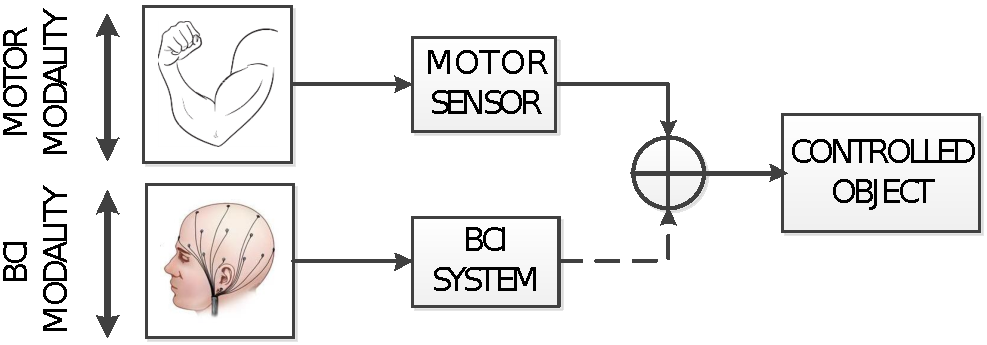
\includegraphics[width=0.8\columnwidth]{Figures/hBCI2.pdf}
    \caption{Hybrid BCI system integration. The motor abilities of the user are the primary controller of the system, using adapted interfaces (here: 3D touchless interface). The brain-computer interface (here: SSVEP) provides a complementary communication channel and is designed to trigger specific actions.}
    \label{fig:hBCI}
\end{figure}

The second modality, which is based on the EEG, is used to provide an additional command, giving alternative control options to the user, or a special command to activate a common and repetitive task.
In this work, the continuous control is achieved by means of a touchless interface and the BCI modality relies on SSVEP. 

\section{Touchless Interface}
\label{sec:touchless-interface}

%- First to equip exoskeleton
%- Then as a general interface that offers many degree of freedom without grasping. It can suitably replace the joistick
There are a number of neurodegenerative diseases that affect large muscles. Some result in loss of strength in the hands and the fingers.
For instance, people with amyotrophic lateral sclerosis may have their hands and fingers weakened and lose their grasping capacity.
Such patients cannot use most of the existing computer input devices such joysticks and mouses that require a certain degree of grasping. 
The \emph{touchless} interface used in this work is designed for such patients. 
It requires no physical contact and no grasping.
The interface embeds five infrared (IR) sensors which could be setup in different spatial positions, according to the user requirements.
Each IR-sensor consist of a pair of IR transmitter-receiver (Tx/Rx). 
The sensors are placed spatially around a user's arm such that a slight hand movement will alter the pattern of reflected IR beams.
The interface is configured to detect six hand positions for six commands namely up, down, left, right, forward, and backward.
To these is added a resting position.
The position is chosen to be intuitive and coherent with the command. They are further tuned to fit user hand movement capacities through a training phase where the subject is asked to perform movements corresponding to the six positions for a number of times.

\begin{figure}[h!]
\centering
\subfigure[]{
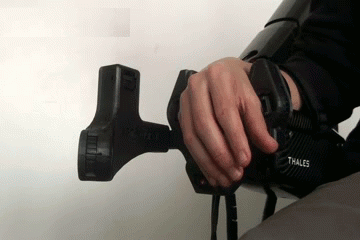
\includegraphics[width=0.3\textwidth]{Figures/left}
\label{fig:ir-left}
}
\subfigure[]{
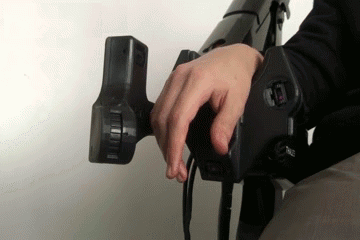
\includegraphics[width=0.3\textwidth]{Figures/right}
\label{fig:ir-right}
}
\subfigure[]{
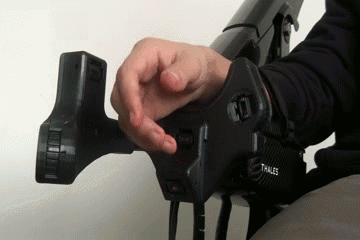
\includegraphics[width=0.3\textwidth]{Figures/up}
\label{fig:ir-up}
}
\subfigure[]{
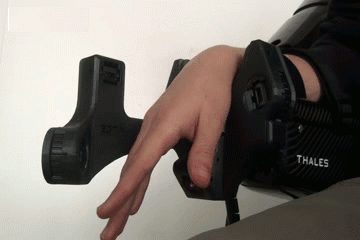
\includegraphics[width=0.3\textwidth]{Figures/down}
\label{fig:ir-down}
}
\subfigure[]{
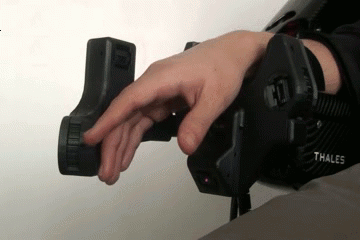
\includegraphics[width=0.3\textwidth]{Figures/front}
\label{fig:ir-front}
}
\subfigure[]{
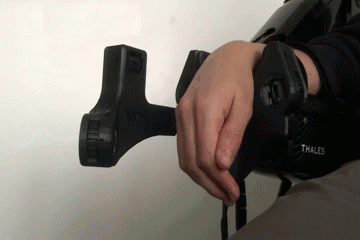
\includegraphics[width=0.3\textwidth]{Figures/rear}
\label{fig:ir-rear}
}
\subfigure[]{
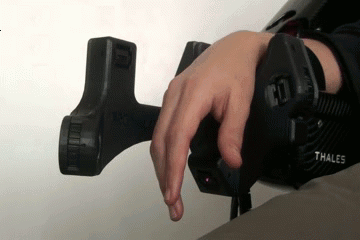
\includegraphics[width=0.3\textwidth]{Figures/rest}
\label{fig:ir-rest}
}
\caption{The 3D touchless interface and a user's hand positions for different commands: (a) left, (b) right, (c) up, (d) down, (e) forward, (f) backward, (g) rest. The IR-sensors are in the black plastic housing on the right side of the hand and around the wrist. Another symmetrical plastic housing has been realised for left-handed users.} 
\label{fig:3D-touchless}
\end{figure}   

The control system relies on an iterative $k$-Nearest Neighbours (kNN) scheme to learn hand poses of each user. 
Firstly, the iterative kNN scheme requires a fast calibration phase to learn the different hand poses, here seven (six for the directions and one for the resting position). 
The outliers and ambiguous examples are excluded from the training examples.
Secondly, the algorithm continuously adapts to the received signal, labelling new examples change the  set of neighbours.
This algorithm is able to track the changes of the user's hand pose, providing an online adaptation to the behavioural modifications induced by tiredness. 
For more details on the algorithm, see\citep{martin_fast_2012}.
The six hand positions recognised by IR-interface is used to control a four degrees-of-freedom robotic arm exoskeleton developed in the \emph{ESTA} project \citep{baklouti_force_2008} to compensate for motor deficiency in the upper limb (Figure~\ref{fig:esta-expe-setup}). 
More generally, it can be used by patients as well as healthy subjects in applications where navigation in a 3D Euclidean space is needed.  

\section{SSVEP-based BCI}
\label{sec:ssvep-bci}

\subsection{Material and EEG Recording}
\label{subsec:material-recording}
The g.Mobilab+ device (shown in Figure \ref{fig:acquisition-system}) is used for recording EEG at 256~Hz on 8 channels.

\begin{figure}[!h]
    \centering
    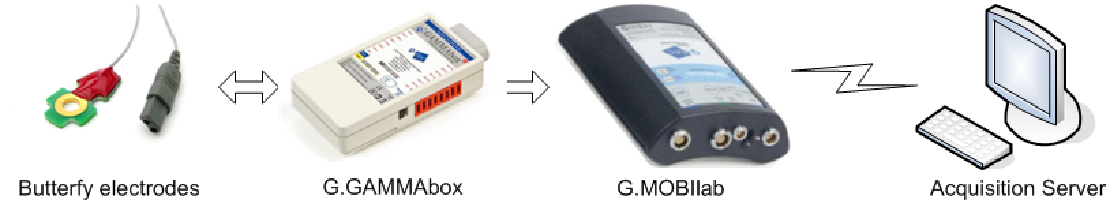
\includegraphics[width=0.8\columnwidth]{Figures/acquisition-system.pdf}
    \caption{\footnotesize{Acquisition material, the EEG is recorded with electrodes, the signal is amplified and sent to a computer running OpenVIBE.}}
    \label{fig:acquisition-system}
\end{figure}

For SSVEP stimulation, flash stimulus technique has been chosen. 
To avoid limitations imposed by refresh rate of computer screens, a microcontroller is set up to  flash stimuli with light-emitting diodes (LED) at frequencies $F =\{13, 17, 21\}$~Hz. %, 17~Hz, and 21~Hz.
The device has been controlled and the LED blinking is precise up to the millisecond.
The eight electrodes are placed according to the 10/20 system on Oz, O1, O2, POz, PO3, PO4, PO7 and PO8. 
The ground was placed on Fz and the reference was located on the right (or left) ear lobe.

In this study, 12 male and female subjects aged between 20 and 32 years participated in the experiment. 
Informed consent was obtained from all subjects, each one has signed a form attesting their consent. 
The subject sits in an electric wheelchair, his right upper limb is resting on the exoskeleton (Figure~\ref{fig:esta-expe-setup}). 
The exoskeleton is functional but is not used in the offline recordings.

\begin{figure}[!t]
    \centering
    %\pgfimage[interpolate=true,width=\linewidth]{Figures/IR_interface}
    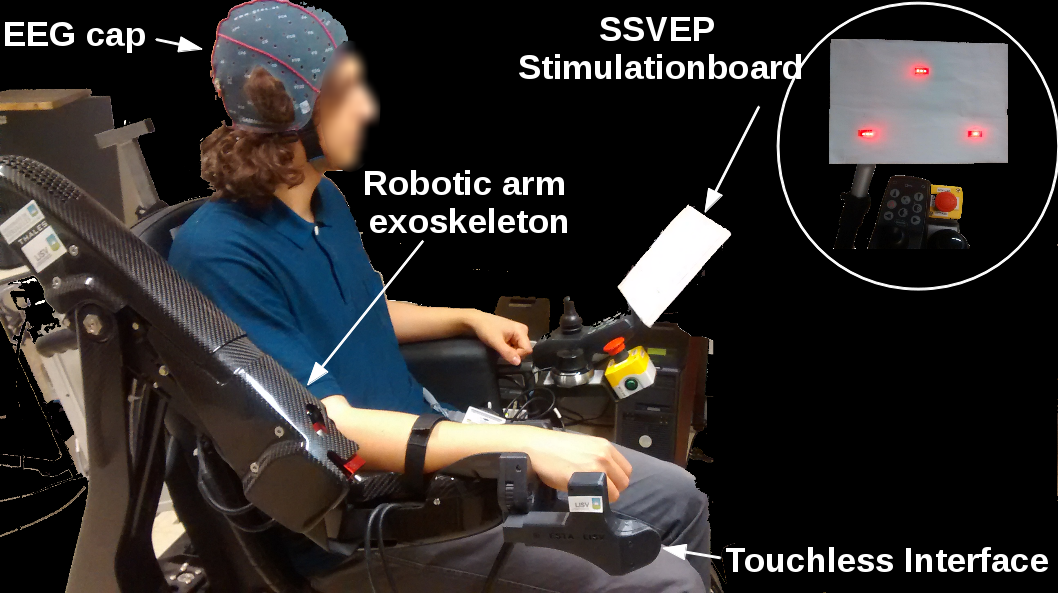
\includegraphics[width=0.8\columnwidth]{Figures/esta-expe}
    \caption{Experimental setting: subject sitting on an electric wheelchair equipped with a robotic arm exoskeleton. During offline recordings, the exoskeleton and the touchless interface are disabled; the subject performs the SSVEP task as prompted by audio cues.}
    \label{fig:esta-expe-setup}
\end{figure}

A panel of size 20x30 cm is attached on the left side of the chair, with three groups of four LEDs blinking at different frequencies. 
Despite the panel being on the left side, users can see it without moving their head. 
The subjects were asked to sit comfortably in the wheelchair and to follow the auditory instructions, they could move and blink freely.
A sequence of trials is proposed to the user. 
A trial begins by an audio cue indicating which LED to focus on, or to focus on a fixation point set at an equal distance from all LEDs for the reject class. 
A trial lasts five seconds and there is a three second pause between each trial. 
The evaluation is conducted during a session consisting of 32 trials, with 8 trials for each frequency and 8 trials for the reject class (or resting class), \textit{i.e.} when the subject is not focusing on any specific blinking LED.

The experiments were conducted at the \emph{Laboratoire d'Ing\'{e}nierie des Syst\`{e}mes de Versailles} (LISV) of the Universit\'{e} de Versailles Saint-Quentin-en-Yvelines, Paris-Saclay. 

\subsection{Signal Processing}

The measured EEG signal is treated with a processing pipeline that offers state-of-the art BCI performance.
EEG epochs of three seconds are gathered every 0.5 second. 
Each epoch is filtered between 12 Hz and 45 Hz to discard irrelevant bands while allowing all stimulation frequencies and their first harmonics. 

A spatial filter is then designed based on CCA method described in Section~\ref{subsubsec:cca}.
Unlike the work of \citep{lin_frequency_2006}, which propose to rely on the correlation coefficient of CCA for processing SSVEP signals, in this work CCA is only applied to determine the spatial filter $w_{\X}$.


%A spatial filter is then designed based on CCA. 
%Let $\X \in \Re^{\dc \times \dt}$ be the obtained EEG trial, where $\dc$ is the number of channels and $\dt$ the number of samples in the trail. 
With the signal being recorded at 256 Hz with eight electrodes, the size of a 3-second EEG trial is $8 \times 768$ ($\X \in \Re^{8 \times 768}$). And let $Y \in \Re^{H \times \dt}$ be a multivariate signal representing the SSVEP stimulation signal.
As described in Section~\ref{subsubsec:cca}, CCA finds the mappings $\w_{\X}, \w_{Y} \in \Re^{8}$ that maximises the correlation between the $\w_{\X}^T \X$, and $\w_{Y}^T Y$.
The signal $\x = \w_{\X}^T \X$ is a linear combination of all the electrodes and is expected to maximise the correlation with a hypothetically perfect neural response, that is the sinusoids of $Y$.
A similar approach can be found in~\citep{spuler_one_2012} but in a different context and using $\x$ to generate exemplars for supervised learning.
After filtering, a multiclass SVM classifier with RBF kernels is used for classification (refer to Section \ref{subsubsec:svm}). 
It is given as input the power spectral densities extracted from the spatially filtered signal $\x$, and output a class $\ci \in \left\lbrace 13 \mathrm{Hz}, 17 \mathrm{Hz}, 21\mathrm{Hz}, resting \right\rbrace$.
The LIBSVM \citep{chang_libsvm:_2011} package is used for SVM implementation.

\section{Applications}

The described approach is validated in two contexts: a Virtual Environment (VE) for the navigation of a helicopter shown in Figure~\ref{fig:online-VE-setup}, and an exoskeleton arm control task shown in Figure~\ref{fig:esta-expe}.
In the VE, the user is asked to reach three waypoints.
Three specific locations are identified in the VE to serve as \emph{shortcuts}. 
In previous works, locations of this nature have been used as a predefined final destination~\citep{lotte_exploring_2010}, while we only use them as shortcuts. 
%They are limited in number to feat the limited number of commands that BCI usually provide. 
After reaching these locations using BCI commands, the user could reach any position using the 3D-touchless interface. 
%is given the option of reaching an infinite number of destinations using the 3D-touchless interface. 

The approach with the exoskeleton arm bears some similitude with the VE navigation task. 
The arm is controlled with the 3D-touchless interface.
Common arm movements performed by the user are predefined (e.g. reaching the mouth or a resting position). 
The BCI shortcut trigger the automatic arm movement to these positions.
 
The hybrid scheme is especially well suited for exoskeleton arm control task: 
%For the robotic arm, this is of essential importance.
as the arm is continuously controlled by the 3D touchless interface, once the user has grabbed an object (e.g. a glass of water), she will no longer be able to move her hand freely to control the touchless interface. 
The BCI command allows to overcome this limitation by activating predefined movements.

\section{Experimental Results}
\label{sec:hBCI-results}
       
This section describes the results obtained with the proposed system.
Out of twelve subjects who participated in the offline EEG recording, only five participated in the online experiment in the virtual environment.
%Five subjects out of participated in the experiments. 
One of the subjects is hemiplegic and the four others are healthy. 
The first section is dedicated to the assessment of the proposed online detection of SSVEP algorithm.
The second section provides the results obtained using the hybrid system for a navigation task in a virtual environment.
The last section explained how the system has been implemented on an embedded system for an exoskeleton arm control task.

\subsection{Validation of Proposed SSVEP Algorithm}
\label{sec:resssvep}

\newcommand{\win}{\ensuremath{t_W}}

Before using the BCI subsystem in online mode, a calibration phase is needed to compute the CCA spatial filter and training the SVM classifier.
During the calibration phase, a sequence of trials is proposed to the user.
%A trial begin by an audio cue indicating which LED to focus on, or to focus on a fixation point set at an equal distance from all LEDs for the reject class.
%A trial last 5 seconds and there is a 3 second pause between each trial.
%The evaluation is conducted during a session consisting of 32 trials, with 8 trials for each frequency $f \in F$ and 8 trials for the reject class, \textit{i.e.} when the subject is not focusing on any specific blinking LED. 
The online classification is done every 0.5 second, using a $\win = 3$~s window of EEG signals. 
An audio feedback indicates the predicted class to the user. %success or failure in the classification. 
%A classification is done every 2 second on the latest EEG sample of 3 seconds.  
%The classification accuracies are given in table~\ref{tab:online_accuracy}.

Figure~\ref{fig:error_rate} shows the online BCI classification performances for each prediction made every 0.5 second, starting at $t=t_0+\win$, that is three seconds after the beginning of the trial $t_0$. 
The y-axis indicates the error rate for each of the five subjects.
The results demonstrate that the proposed algorithm is very robust and provides a very reliable response after $t+2$~s with a small mean error rate for all subjects. 

To further evaluate the algorithm, it is important to consider that the loss function is not uniform. 
If the algorithm detects a reject class instead of a specific class, the consequences are not as bad as a wrong prediction: e.g. detecting 13~Hz instead of 17~Hz, as the user needs only to concentrate half a second on the chosen LED before the system make another prediction.
Thus we propose the following accuracy measure, similar to a precision score.
For each trial, we consider the first class prediction at time $t$: if this is correct the accuracy is increased, if this is false the accuracy is decreased.
If the prediction is the reject class, the accuracy measure is only postponed on the next time segment.
Figure~\ref{fig:accuracy} displays the results of this measure for all subjects.
The accuracy is above 70\% for almost all subjects and it can be seen that the algorithm provides almost immediately the correct answer.
%Table~\ref{tab:online_accuracy} summarizes the maximal accuracy achieved for each subject.

At last, we compare the proposed algorithm with classical SSVEP approaches in Table~\ref{tab:none_ica_cca}, using an offline evaluation  for each subject. 
The baseline is a comparison with a SVM using the PSD of the EEG signal, that is without applying the CCA spatial filter.
A classical methodology is to rely on ICA to extract the main components of the signal and to provide these components to the SVM classifier.
Table~\ref{tab:none_ica_cca} shows that the proposed algorithm yields the best results.

% with a plot of the average classification error rate over a 6.5 seconds trial, computed every 0.5 second for each subject.
% On Figure~\ref{fig:accuracy}, the average accuracy convergence over a 6.5 second trial is plotted for each subject. 
% To evaluate the impact of CCA on the classification, we compare, in table ~\ref{tab:none_ica_cca}, the performance of this technique to the one obtained when no spacial filter is used and the one where ICA is used instead. This was than offline. 

\begin{figure}[!t]
    \centering
    %\pgfimage[interpolate=true,width=0.9\columnwidth]{Figures/error_rate.pdf}
    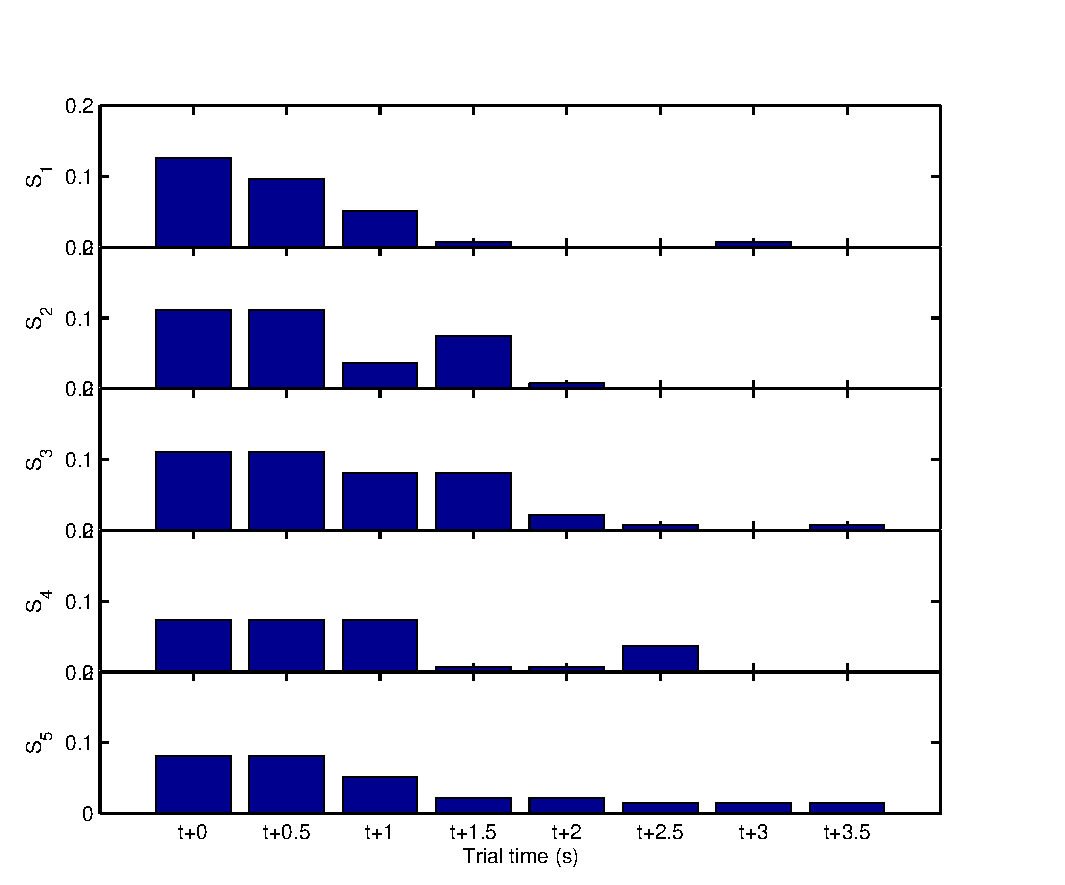
\includegraphics[width=0.8\columnwidth]{Figures/error_rate.pdf}
    \caption{Evaluation of the online performances of the proposed BCI algorithm. The error rates for all five subjects are indicated as a function of time, with $t$+0 indicating the first prediction made (after $\win = 3$~s). The error rates are averaged on all classes.}
    \label{fig:error_rate}
\end{figure}

 \begin{figure}[!t]
    \centering
    %\pgfimage[interpolate=true,width=0.9\columnwidth]{Figures/accuracy.pdf}
    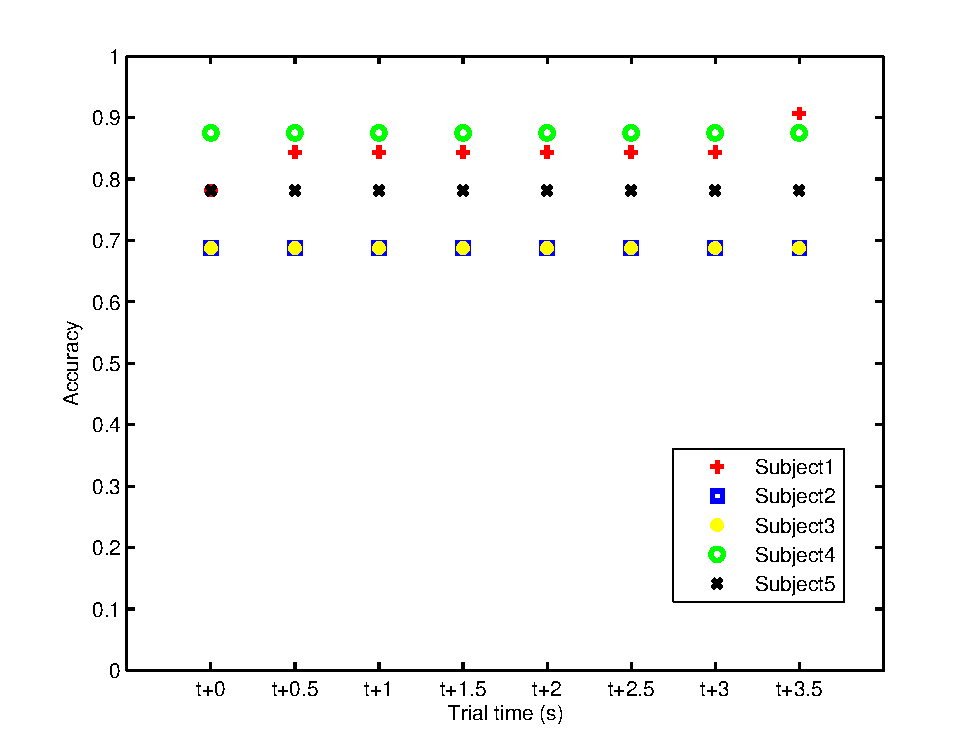
\includegraphics[width=0.8\columnwidth]{Figures/accuracy.pdf}
    \caption{Assessment of the accuracy of classification depending on the time of the prediction. On x-axis, $t$+0 indicates the first prediction made three seconds after the start of a trial. The results are averaged on all trials for each subject. Subject 1 is the only one to present a slight increase of the classification accuracy. For all other subjects, the algorithm proposes a correct answer as the first prediction.}
    \label{fig:accuracy}
\end{figure}

% \begin{table}[!t]
% \centering
% %\ra{1.3}
% \begin{tabular}{@{}lrrrrr@{}}\toprule
% & \multicolumn{1}{c} {Subject1} & \multicolumn{1}{c} {Subject2} & \multicolumn{1}{c} {Subject3} & \multicolumn{1}{c} {Subject4} & \multicolumn{1}{c}{Subject5} \\ \midrule
% Accuracy (\%) & 84.50 & 68.75 & 68.75 & 87.50 & 78.25 \\
% \bottomrule
% \end{tabular}
% \caption{Online accuracy achieved for each subject}
% \label{tab:online_accuracy}
% \end{table}

%\textcolor{red}{table~\ref{tab:online_accuracy} should be updated according to final value of ploss} 


\begin{table}[!t]
\caption{Comparison with other algorithms}
\centering
%\ra{1.3}
\begin{tabular}{@{}lrrrrr@{}}\toprule
& \multicolumn{1}{c} {Subject1} & \multicolumn{1}{c} {Subject2} & \multicolumn{1}{c} {Subject3} & \multicolumn{1}{c} {Subject4} & \multicolumn{1}{c}{Subject5} \\ \midrule
%\cmidrule{2-3} \cmidrule{4-6} \cmidrule{7-9} \cmidrule{10-12}
Baseline& 81.3 & 88.3  & 80.0 & 75.0 & 79.2 \\ \midrule
ICA & \textbf{100} & 88.3  & 91.7 & \textbf{93.3} & 95.0 \\ \midrule
CCA & \textbf{100} & \textbf{100}  & \textbf{97.5} & \textbf{93.3} & \textbf{96.7} \\
\bottomrule
\end{tabular}
\label{tab:none_ica_cca}
\end{table}

\subsection{Experiments in Virtual Environment}
\label{sec:expve}

\begin{figure}[!t]
    \centering
    %\pgfimage[interpolate=true,width=0.8\columnwidth]{Figures/online-expe-setup.jpg}
    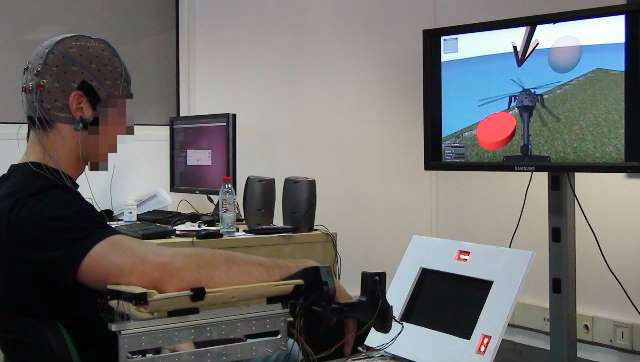
\includegraphics[width=1\columnwidth]{Figures/online-expe-setup.jpg}
    \caption{Experiment in the virtual environment. Here the subject is using the 3D touchless interface with his right hand and the SSVEP LEDs are put in front of him. The screen displays a helicopter in the virtual environment. The subject should pass through all waypoints, materialised by red (or grey) disks on the screen. When the subject triggers a shortcut, the helicopter is automatically moved to a location materialised by the transparent ball.}
    \label{fig:online-VE-setup}
\end{figure}
 
For the navigation task in the virtual environment, the assessment is based on the time spent and the distance travelled during the experiment for four subjects.
%The results in the VE navigation is presented as an evaluation of time spent and trajectory covered to reach the 3 destinations. 
These results are shown in Table~\ref{tab:distime}. 
The time is indicated in seconds and the distance in metric units. 
Each subject has performed three experiments: in the first experimental condition, the subject should rely only on the 3D touchless interface (`None' in Table~\ref{tab:distime}).
In the second one, shortcuts are available and are triggered by the BCI subsystem (BCI-S).
In the last experimental condition, the subject could trigger a shortcut using a keyboard (KB-S).
The fourth subject is hemiplegic and she could not use the keyboard with her spare hand.
Thus, her results do not include the last experimental condition. 

In Table~\ref{tab:distime}, next to the BCI and keyboard shortcut, a percentage indicates the relative improvement compared to the reference experiment (without shortcut).
It could be seen that distance covered is almost equivalent with BCI shortcuts and keyboard shortcuts, which is the expected results as users have activated the shortcut each time it was possible. 
When the shortcuts are activated by the BCI, the task is slower than when using the keyboard. 
This effect is mainly caused because the subject need to focus at least three seconds on a blinking LED before triggering the shortcut. 
%Nonetheless, it could be seen than the subject with hemiplegia could not use the keyboard with his spare hand and thus he could not rely on this alternative to trigger the shortcut.


% , the time spent and the distance covered to reach the destinations when using the 3D touchless interface alone (No short.), are compared with those achieved by using the combination of the touchless interface and shortcuts taken with BCI commands (BCI short.). To evaluate the delay that BCI inserts in the shortcut taking approach, the result are also compared to those achieved when shortcuts are activated by pressing a key on the keyboard (Key short.). The results of 4 subject are shown in table~\ref{tab:distime}. The fourth subject is hemiplegic. His results do not include those of shorcuts activated with the keyboard. Next to BCI short. and Key short. are they respective improvement (increase in performance) factor in percentage compared to the performance of the touchless interface alone.

\begin{table}[!ht]
\centering
\caption{Distance covered and duration of experiments, without shortcuts (None), with BCI-activated shortcuts (BCI-S) and with keyboard-activated shortcuts (KB-S).}
\ra{1.3}
\begin{tabular}{@{}ccrrr@{}}
\cline{1-5}
&  & None & BCI-S (inc. \%). & KB-S (inc. \%). \\ \cline{1-5}
\multicolumn{1}{ c }{\multirow{2}{*}{Subject 1} } &
\multicolumn{1}{ c }{Time} & 108.9 & 68.3 (37.3\%) & 53.56 (50.8\%)      \\ \cline{2-5}
\multicolumn{1}{ c  }{}                        &
\multicolumn{1}{ c }{Distance} & 1367.7 & 538.2 (60.6\%) & 535.0 (60.9\%) \\ \cline{1-5}
\multicolumn{1}{ c }{\multirow{2}{*}{Subject 2} } &
\multicolumn{1}{ c }{Time} & 99.2 & 74.7 (24.7\%) & 50.5 (49.1\%) \\ \cline{2-5}
\multicolumn{1}{ c  }{}                        &
\multicolumn{1}{ c }{Distance} & 1469.4 & 529.1 (64.0\%) & 549.0 (62.6\%) \\ \cline{1-5}
\multicolumn{1}{ c }{\multirow{2}{*}{Subject 3} } &
\multicolumn{1}{ c }{Time} & 105.5 & 63.4 (39.9\%)& 50.4 (52.2\%) \\ \cline{2-5}
\multicolumn{1}{ c  }{}                        &
\multicolumn{1}{ c }{Distance} & 1447.3 & 627.6 (56.6\%) & 542.1 (62.5\%) \\ \cline{1-5}
\multicolumn{1}{ c }{\multirow{2}{*}{Subject 4} } &
\multicolumn{1}{ c }{Time} & 125.6 & 70.4 (43.9\%) & --       \\ \cline{2-5}
\multicolumn{1}{ c  }{(hemiplegic)}                        &
\multicolumn{1}{ c }{Distance} & 1490.8 & 598.9 (59.8\%) & --     \\ \cline{1-5}
\end{tabular}  
\label{tab:distime}
\end{table}
%%\newcommand{\ra}[1]{\renewcommand{\arraystretch}{#1}}
%\begin{table*}\centering
%\ra{1.3}
%\begin{tabular}{@{}rrrcrrcrrcrr@{}}\toprule
%& \multicolumn{2}{c}{Subject1} & \phantom{abc}& \multicolumn{2}{c}{Subject2} & 
%\phantom{abc} & \multicolumn{2}{c}{Subject3} & \phantom{abc} & \multicolumn{2}{c}{Subject4}\\
%\cmidrule{2-3} \cmidrule{4-6} \cmidrule{7-9} \cmidrule{10-12}
%& Time & Distance  && Time & Distance && Time & Distance && Time & Distance\\ \midrule
%Touchless alone & 108.9 & 1367.7 && 99.2 & 1469.4  && 105.5 & 1447.3 && 125.6 & 1490.8 \\
%BCI shortcut & 68.3 & 538.2 && 74.7 & 529.1  && 63.4 & 627.6 && 70.4 & 598.9 \\
%Keyboard shortcut & 53.56 & 535.0 && 50.5 & 549.0  && 50.4 & 542.1 && -- & -- \\
%\bottomrule
%\end{tabular}
%\caption{Distance covered and duration of tasks}
%\label{tab:distime}
%\end{table*}

% The time spent to reach the destinations while using shortucts, BCI or keyboard, is shorter than the time spent when using the touchless interface alone. The difference could be greater in a larger environment. Using a shortcut is definitely a way of fastening and easing the the task. Both BCI and keyboard shortcuts allow users to take predefined optimal paths. They reduce the distance covered by almost equal factors. It is clear when comparing the time of BCI shortcut against the one of keyboard shortcut, that BCI insert a significant delay. Since disabled users, e.g. hemiplegic, cannot reach the keyboard, performances of BCI shortcuts are of great significance.      

\subsection{Application to Exoskeleton Arm Control}
\label{sec:estares}

The proposed system has been applied to the ESTA exoskeleton arm control.
This assistive device is designed to compensate shoulder and elbow deficiencies occurring in degenerative diseases.
The subject controls the exoskeleton arm with the touchless interface and the BCI shortcuts allow to reach predefined positions, such as a resting or a close-to-mouth positions.
In the case of the hemiplegic subject (who cannot use her left arm and hand), the BCI subsystem is the only possibility to control the exoskeleton with an object in hand.
This example illustrates the complementary aspect of the two interfaces, the physical and the brain one.

Figure \ref{fig:esta-expe} illustrates an application of the proposed hybrid interface on the ESTA chair.
The user is seated in an environment where he can perform daily life routine. 
In this case, next to a table where a phone and a glass of water are placed on (to represent objects that are commonly used).
The user can reach to the table, and pick an object of his choice and manoeuvre it around. His arm is supported with the robotic exoskeleton and he is given the touchless interface and the BCI in the hybrid multimodal framework to control it.   
As with in the VR environment, regions of interest can be defined in a daily life environment. 
These regions are the most visited and trajectories leading to them can be optimised and recorded. 
In the current experiment, the table and the user's face (mouth), and the resting positions are defined as regions of interest. 
Their trajectories are optimised, recorded and can be triggered automatically.
In this way, the user can use BCI commands to trigger movement to regions of interest. 
The touchless interface can then be used for it continuous control to reach local positions.
The IR interface can be turned on and off using a BCI command. 
This will allow the user to move his hand even when he does not intend to send a command to the touchless interface.  

\begin{figure}[h!]
\centering
\subfigure[]{
\includegraphics[width=0.45\textwidth]{Figures/esta01}
\label{fig:esta01}
}
\subfigure[]{
\includegraphics[width=0.45\textwidth]{Figures/esta02}
\label{fig:esta02}
}
\subfigure[]{
\includegraphics[width=0.45\textwidth]{Figures/esta03}
\label{fig:esta03}
}
\subfigure[]{
\includegraphics[width=0.45\textwidth]{Figures/esta04}
\label{fig:esta04}
}
\caption{Subject sitting on the ESTA wheelchair. His arm is supported by the exoskeleton, and the left hand is lying on the touchless interface. On his right-hand side is the SSVEP stimulation board. He is fitted with an EEG cap for brain signals recording. Next to the exoskeleton, an object is put on a table. (a) The subject is in resting position. He is gazing at the 17 Hz LED to trigger an automatic trajectory to the table. (b) Subject has reached the table and is using the touchless interface to reach and grab the glass (c) Glass in hand, the user gazing at the 13 Hz LED to activate the automatic trajectory to mouth. (d) The arm reaches the mouth while the touchless interface is deactivated.} 
\label{fig:esta-expe}
\end{figure} 
%\begin{figure}[!t]
%  \centering
%  %\pgfimage[interpolate=true,width=0.8\columnwidth]{Figures/online-esta.jpg}
%  \includegraphics[width=0.8\columnwidth]{Figures/online-esta.jpg}
%  \caption{The ESTA arm exoskeleton with the proposed system: a 3D-touchless interface and the SSVEP-based BCI.}
%  \label{fig:online-esta-setup}
%\end{figure}


%%%%%%%%%%%%%%%%%%%%%%%%%%%%%%%%%%%%%%%%%%%%%%%%%%%%%%%%%%%%%%%%%%%%%%%%%%%%%%%%
\section{Conclusion}
\label{hBCI-conclusion}

In this chapter a new methodology for designing hybrid systems was proposed. It uses a brain interface and physical interface specifically design to fit the user's needs. 
The main goal of this hybrid system is to assist people with motor disabilities or muscular diseases, by proposing a system that adapts to their individual needs, and makes use of their residual abilities.
The BCI is integrated in the system as a secondary modality, which is used to trigger specific behaviour or predefined actions.

A first contribution is to propose an implementation of such a system using a 3D touchless interface and a SSVEP-based BCI.
This implementation gathers the two interfaces in a multimodal system which benefits from both the brain and motor signals.
The second contribution is to describe a novel algorithm for processing SSVEP-based EEG signals, with stable results, even when computed in an online setup.
This algorithm is compared to other existing solutions and an experimental assessment of its validity is conducted.

The full system is evaluated on a 3D  navigation task in virtual environment. 
The results demonstrate that the system is functional and could be used to assist people in various contexts.
The system is lastly used to control the ESTA arm exoskeleton: the system is functional and could be adapted for controlling other  assistive devices.

Although a good classification accuracy is achieved with the proposed method based on CCA and SVM, this work focuses more on BCI framework to improve the BCI usability and adaptability to the physical needs of subjects. The proposed framework answers the problem of variability in physical aptitude amongst patients and users of BCI.
Future work will be focused on the signal processing and machine learning methods that tackle variability in the brain response and in the experimental environment. 
%This continuous adaptation to the user's condition could help 
%speak of the aspect of maintaining both motor activity while lightening and/or fastening the task to be achieved with BCI.
% ------------------------------------------------------------------------
% -*-TeX-*- -*-Hard-*- Smart Wrapping
% ------------------------------------------------------------------------
%%% Literature Survey --------------------------------------------------

%\addtolength{\topmargin}{-.875in}
%\addtolength{\textheight}{.875in}
%\footskip
%\nonumchapter{Literature Survey}
\chapter{Riemannian Geometry for Brain-Computer Interfaces}
\label{chap:riem-geom-bci}
\epigraph{The history of science has proved that fundamental research is the lifeblood of individual progress and that the ideas that lead to spectacular advances spring from it.}{--- \textup{Sir Edward Appleton}}

\section{Riemannian Manifold of Symmetric Positive-Definite Matrices}
\label{sec:riemann-manifold}

A $\totd$-dimensional \emph{manifold} $\GenMa$ is a Hausdorff space for which every point has a neighbourhood that is homeomorphic to an open subset of $\Re^\totd$ \citep{jost_riemannian_2011}.
When a tangent space is defined at each point, $\GenMa$ is called a differential manifold. 
A \emph{geodesic} $\gamma$ is the shortest smooth curve between two points, $\P_1$ and $\P_2$. 
The tangent space $T_\P\GenMa$ at point $\P$ is the vector space spanned by the tangent vectors of all geodesics on $\GenMa$ passing through $\P$. 
A \emph{Riemannian} manifold is a manifold endowed with an inner product defined on the tangent space, which varies smoothly from point to point.  %at each point is a finite-dimensional Euclidean space. 

For the rest of this chapter, we will restrict to the analysis of the manifold $\Ma$ of  the $\dc\times\dc$ symmetric positive-definite (SPD) matrices, defined as:
\begin{equation*}
	\label{eq:rm}
  \Ma = \left\{ \P \in  \Re^{\dc\times\dc} : \P = \P^\intercal \text{ and } x^\intercal \P x > 0, \forall x \in \Re^{\dc} \backslash 0 \right\} \ . %\nonumber
\end{equation*}
The tangent space $T_{\P}\Ma$ is identified to the Euclidean space of symmetric matrices:
\begin{equation*}
  \label{eq:sy}
  \Sy = \left\{ \S \in \Re^{\dc\times\dc} : \S = \S^\intercal \right\} \ . %\nonumber
\end{equation*}
The dimension of the manifold $\Ma$, and its tangent space $T_{\P}\Ma$, is $\totd = \dc(\dc+1)/2$.

The mapping from a point $\S_i$ of the tangent space to the manifold is called the exponential mapping $\Exp{\P}(\S_i)$: $T_{\P}\Ma \rightarrow \Ma$ and is defined as:
\begin{equation}
	\label{eq:exp_r}
	\Exp{\P}(\S_i) = \P^{\frac{1}{2}}\Expm(\P^{-\frac{1}{2}}\S_i \P^{-\frac{1}{2}})\P^{\frac{1}{2}} \ .
\end{equation}  
Its inverse mapping, from the manifold to the tangent space is the logarithmic mapping $\Log{\P}(\P_i)$: $\Ma \rightarrow T_{\P}\Ma$ and is defined as:
\begin{equation}
	\label{eq:log_r}
	\Log{\P}(\P_i) = \P^{\frac{1}{2}}\Logm(\P^{-\frac{1}{2}}\P_i \P^{-\frac{1}{2}})\P^{\frac{1}{2}} \ .
\end{equation} 
$\Expm(\cdot)$ and $\Logm(\cdot)$ are the matrix exponential and matrix logarithm respectively.
The computation of these operators is straightforward for SPD matrices of $\Ma$. %for symmetric matrices of $\Sy$. % in $T_{\P}\Ma$ or $\Ma$.  
They are obtained from their eigenvalue decomposition (EVD): 
\begin{displaymath}
  \begin{split}
    \P &= U\, \text{diag}(\ev_1, \dots, \ev_\dc)\, U^\intercal \ , \\
    \Expm(\P) &= U\, \text{diag}(\exp(\ev_1), \dots, \exp(\ev_\dc))\, U^\intercal \ , \\
    \Logm(\P) &= U\, \text{diag}(\log(\ev_1), \dots, \log(\ev_\dc))\, U^\intercal \ ,
  \end{split}
\end{displaymath}
where $\ev_1, \dots, \ev_\dc$ are the eigenvalues and $U$ the matrix of eigenvectors of $\P$.
As any SPD matrix can be diagonalised with strictly positive eigenvalues, $\Logm(\cdot)$ is always defined.
Similarly the square root $\P^{\frac{1}{2}}$ is obtained as:
\begin{equation*}
  \label{eq:sqm}
  \P^{\frac{1}{2}} = U\, \text{diag}(\ev_1^{\frac{1}{2}}, \dots, \ev_\dc^{\frac{1}{2}})\, U^\intercal \ , %\nonumber
\end{equation*}
and is unique. The same goes for $\P^{-\frac{1}{2}}$.

The tangent vector of the geodesic $\gamma(t)$ between $\P_1$ and $\P_2$, where $\gamma(0) = \P_1$ and $\gamma(1) = \P_2$ is defined as:
\begin{equation}
  \label{eq:tan_geo}
  v = \overrightarrow{\P_1 \P_2} = \Log{\P_1}(\P_2) \, . 
\end{equation}

%A Riemannian distance between $\P_1$ and $\P_2$ can thus be defined as~\cite{moakher2005differential}:  
%\begin{equation}
%	\label{eq:dist_r}
%	\distR(\P_1,\P_2) = \|\Logm(\P_1^{-1}\P_2)\|_F = \left[\sum_{\chI=1}^{\dc}\log^{2}\lambda_{\chI}\right]^{1/2} ,
%\end{equation}
%where $\lambda_\chI$, $\chI = 1, \dots, \dc$, are the eigenvalues of $\P_1^{-1}\P_2$.
%From Eq.~\eqref{eq:dist_r}, the geometric mean of $\Nb$ points $\P_\nb$ on the manifold, $\nb = 1, \dots , \Nb$, can be defined as the point that minimizes the sum of squared distances to all $\P_\nb$:
%\begin{equation}
%\label{mean_r}
%\Rm(\P_1, \dots, \P_\Nb) = \argmin_{\P \in \Ma} \sum_{\nb=1}^{\Nb} \distR^2(\P_\nb,\P) \ .
%\end{equation}
%%\|\log(P_k^{-1}P)\|_F^2
%This mean has no closed form, and can be computed iteratively \cite{fletcher2004principal}.
%%Syl: was "This geometric mean" but it could be interpreted as a mean of the product of the terms, that is called a geometric mean.

\section{Covariance Matrix Estimation}
\label{sec:covmat-estimation}

When working with covariance matrices, a crucial point is to correctly estimate the covariance when the number of samples is small or heavily corrupted by noise. 
Several approaches have been proposed to build the covariance matrices, relying on normalisation or regularisation of the sample covariances. 
To assess the quality of the covariance matrices obtained from EEG samples, a comparative study of these estimators is conducted.

%Let $X \in \Re^{p \times n}$ denotes a sample of random variables, where $p$ is the number of variables and $n$ the number of samples, $X = [\x_1 \x_2 \dots \x_n]$
Let $\x_\si \in \Re^{\dc}$, $\si=1, \ldots, \dt$, denotes a sample of a multichannel EEG trial recorded on $\dc$ electrodes. 
$\dt$ is the trial length. 
Let $\X \in \Re^{\dc\times\dt}$ be the EEG trial such as $\X = [\x_1, \ldots, \x_{\dt} ]$.
Under the hypothesis that all $\dt$ samples $\x_\si$ are randomly drawn from a distribution, it follows that $\boldsymbol{x}$ is a variable of random vectors and its expected vector is $\EX = E\{ \boldsymbol{x} \}$ \citep{fukunaga_introduction_1990}. %Fukunaga page 18
The covariance matrix of the random variable $\boldsymbol{x}$ is defined by $\P = E\{ (\boldsymbol{x} - \EX)(\boldsymbol{x} - \EX)^{\intercal} \}$ and is unknown, thus an estimate $\cov{ }$ should be computed.
% The covariance matrix $\P$ of EEG multichannel recording is usually unknown and an estimate $\cov{ }$ should be computed.
%There are many techniques that are used to an estimate $\cov{ }$. 
The choice of the appropriate estimator is crucial to verify that the obtained covariance matrices fulfil the following properties: they should be accurate, SPD, and well-conditioned.
The last property requires that the ratio between the maximum and minimum singular value is not too large.
Moreover, to ensure the computational stability of the algorithm, the estimator should provide full-rank matrices, and its inversion should not amplify estimation errors. 

\subsection{Sample Covariance Matrix Estimator}

The most usual estimator is the empirical \emph{sample covariance matrix} (SCM), defined as: 
\begin{equation}
  \begin{split}
    \cov{scm} & = \frac{1}{\dt-1} \sum_{\si=1}^{\dt} (\x_\si - \xb)(\x_\si - \xb)^\intercal 
		\\
    & = \frac{1}{\dt-1} \X\left( \eye_\dt -\frac{1}{\dt}\unitary_{\dt} \unitary_{\dt}^\intercal \right) \X^\intercal \ ,
  \end{split}  
\end{equation}
where $\xb \in \Re^{\dc}$ is the sample mean vector $\xb = \frac{1}{\dt} \sum_{n=1}^\dt \x_\si $.
In the matrix notation, $\eye_{\dt}$ is the $\dt\times\dt$ identity matrix and $\unitary_{\dt}$ is the vector $[1, \ldots, 1]$.
The SCM is often normalised as~\citep{fukunaga_introduction_1990}:
\begin{equation}
  \label{eq:nscme}
  \cov{nscm} = \frac{\dc}{\dt} \sum_{\si=1}^{\dt} \frac{(\x_\si - \xb)(\x_\si - \xb)^\intercal }{\sigma_{\x_\si}^2} \ ,
\end{equation}
with the inter-channel variance at time $\si$ defined as $\sigma_{\x_\si}^2 = (\x_\si - \xb)^\intercal (\x_\si - \xb)$. % A VERIFIER! OK
Another normalisation techniques could be used. 

This estimation is fast and computationally simple.
However when $\dc \approx \dt$, the SCM is not a good estimator of the true covariance. 
In the case $\dc > \dt$, the SCM is not even full rank.

\subsection{Shrinkage Covariance Matrix Estimators}

To overcome the shortcomings of SCM, the shrinkage estimators have been developed as a weighted combination of the SCM and a target covariance matrix, which is often chosen to be close to the identity matrix, \textit{i.e.} resulting from almost independent variables of unit variance.
\begin{equation}
	\label{eq:shrink}
	\cov{shrink} = \kappa \tarco +(1-\kappa)\cov{scm} \ ,
\end{equation} 
where $0 \leqslant \kappa < 1$.
This estimator provides a regularised covariance that outperforms the empirical $\cov{scm}$ for small sample size, that is $\dc \approx \dt$. 
The shrinkage estimator has the same eigenvectors as the SCM, but the extreme eigenvalues are modified, \textit{i.e.} the estimator is shrunk or elongated toward the average.

The different shrinkage estimators differ in their definition of the target covariance matrix $\tarco$. 
Ledoit and Wolf~\citep{ledoit_well-conditioned_2004} ($\cov{shrink\_ledoit}$ on Figure~\ref{fig:acc_errorbar}) have proposed $\tarco=\mathit{v}\eye_{\dc}$, with $\mathit{v} = \text{Tr}(\cov{scm})$. 
Blankertz~\citep{blankertz_single-trial_2011} ($\cov{shrink\_blank}$) defines $\tarco$ also as $\mathit{v}\eye_{\dc}$ but with $\mathit{v} = \frac{\text{Tr}(\cov{scm})}{\dc}$. 
Sch\"{a}fer ($\cov{shrink\_schaf}$) proposes several ways of defining $\tarco$ depending on the observed $\cov{scm}$~\citep{schafer_shrinkage_2005}.
%The shrinkage estimator shrinks (or enlarges) the sample covariance matrix toward a more \textcolor{red}{circular covariance}. 
%When $\lambda = 1$, the estimated covariance matrix $\hat{\Sigma}$ does not take into consideration the empirical data; and when $\lambda=0$, $\hat{\Sigma}$ is not regularized. 

%
%\subsection{Ledoit Shrinkage}
%Ledoit and Wolf developed a shrinkage estimator $\hat{\Sigma}$ of the covariance $\Sigma$ as a linear combination of the identity matrix and the sample covariance matrix, $\hat{\Sigma}=\rho_1I+\rho_2\SCM $ that minimizes the expected quadratic loss $E[\| \hat{\Sigma}-\Sigma \|]$. $\rho_1$ and $\rho_2$ are the shrinkage parameters defined by scalar functions of the covariance matrix $\Sigma$. Since estimator $\Sigma$ is unobserved, these parameters are estimated from the empirical covariance matrix $\SCM$ as described in [Ledoit 2004]. 
%\subsection{Sch\"{a}fer Shrinkage}
%Sch\"{a}fer and Strimmer proposed a shrinkage estimator based on Ledoit and Wolf work [Ledoit2003]. Their estimator is a weighted combination of the sample covariance matrix $\SCM$ and an estimated covariance target $\mathbf{T}$: $\hat{\Sigma}=\lambda \mathbf{T}+(1-\lambda)\SCM$. $\lambda$ is taken to be the argument that minimizes the squared error loss function, i.e. the Frobenius norm: $L(\lambda) = \| \hat{\Sigma} - \Sigma \|_F^2$. This estimator offers a systematic way to obtain a regularized $\hat{\Sigma}$ that outperforms the empirical $SCM$ and the theoretical $\mathbf{T}$, based on the knowledge of data.
%\subsection{Blankertz Shrinkage}

\subsection{Fixed-Point Covariance Matrix Estimator}

The fixed-point covariance matrix~\citep{pascal_theoretical_2005} is based on the maximum likelihood estimator $\mle$ which is a solution to the following equation:
\begin{equation}
\label{eq:max_lik}
\cov{fp} = \mle = \frac{\dc}{\dt} \sum_{\si=1}^\dt \left( \frac{(\x_\si - \xb)(\x_\si - \xb)^\intercal }{(\x_\si - \xb)^\intercal  \mle^{-1} (\x_\si - \xb)} \right) \ .
\end{equation}
%where $p$ is the normalization: $p = tr(\cov{scm})$. 
%This equation admits a single fixed point $\hat{\mathbf{M}}_{fp}$ as solution. 
As there is no closed form expression to Eq.~\eqref{eq:max_lik}, it can be written as a function of $\mle$: $\fmle(\mle) = \cov{fp}$.
%\begin{equation}
%\label{eq:max_lik_func}
%\fmle(\mle) = \frac{p}{\dc} \sum_{i=1}^\dt \left( \frac{(\x_i-\xb)(\x_i-\xb)^\intercal }{(\x_i-\xb)^\intercal  \mle^{-1} (\x_i-\xb)} \right) \ .
%\end{equation}
$\fmle$ admits a single \emph{fixed point} $\mle^*$, where $\fmle(\mle^*) = \mle^*$, which is a solution to Eq.~\eqref{eq:max_lik}. 
Using $\mle_{0}:=\cov{nscm}$ as the initial value of $\mle $, it is solved recursively as $\mle_{t} \underset{t \to \infty}{\longrightarrow} \mle^{*}$.

\section{Classification of SSVEP Covariance Matrices}
\label{sec:classification-covmat}
%%%%%%%%%%%%%%%%%%%%%%%%%%%%%%%%%%%%%%%%%%%%%%%%%%%%%%%%%%%%%%
\subsection{Machine Learning Approach for Classification}
\label{subsec:fund_class}

From multiple labelled observations, belonging to two or more classes, and a new unlabelled observation, the classification task objective is to assign to the class whose elements share similar properties with the considered observation.
In this article, we make two hypotheses that are commonly acknowledged in EEG: the data distribution is Gaussian and classes have identical dispersions.
Given labelled observations $\x_i$ drawn from two classes ($y_i = 1$ or $y_i=-1$), a simple classification algorithm consists in assigning a previously unseen observation to the class with the closest mean.
This simple algorithm requires only to define a computable distance and mean. %, that could be computed
Assuming that the observations are embedded into a dot product space, \textit{e.g.} Euclidean space, the mean can be expressed as:
\begin{equation}
c_{+} = \frac{1}{m_{+}} \sum_{ \left\lbrace i|y_i=+1 \right\rbrace } \x_i \ ,
\label{eq:mean_eucl1}
\end{equation}
\begin{equation}
c_{-} = \frac{1}{m_{-}} \sum_{ \left\lbrace i|y_i=-1 \right\rbrace } \x_i \ ,
\label{eq:mean_eucl2}
\end{equation}
where $y_i \in \left\lbrace +1, -1 \right\rbrace$ is the label of the training observation $\x_i$, $m_{+}$ and $m_{-}$ the number of positive and negative observations respectively. 
An unseen observation $\x$ is assigned to the class whose mean is the closest. 
This simple geometric classification framework is the founding principle of more complex algorithms such as support vector machines. 
It can be formulated in terms of the dot product $\left\langle \cdot, \cdot \right\rangle$.
If $c=(c_{+}+c_{-})/2$ is the point lying halfway between $c_{+}$ and $c_{-}$, and $w=c_{+}-c_{-}$ the vector connecting $c_{+}$ to $c_{-}$, the class label $y$ of the unseen observation $\x$ is determined by checking whether the vector $\x-c$ connecting $c$ to $x$ make an angle $\alpha < \pi/2$ with $w$.   
This is expressed as:
\begin{equation}
\begin{split}
y &= \mathrm{sgn} \left\langle (\x-c),w \right\rangle \\
  &= \mathrm{sgn} \left\langle (\x-(c_{+}+c_{-})/2),(c_{+}-c_{-}) \right\rangle \\
  &= \mathrm{sgn} (\left\langle \x,c_{+} \right\rangle - \left\langle \x,c_{-} \right\rangle + b)
\end{split}
\label{eq:classif1}
\end{equation}
where $\mathrm{sgn}$ is the sign function.
The offset $b$ vanishes if class means are equidistant to the origin \cite{scholkopf_learning_2001}.

This thesis focuses on a simple classification scheme, which assigns a previously unseen observation to the class with closest mean.
The observations are considered in a different feature space, through their covariance matrices, which is not usual in signal processing for BCI.
Most approaches favour more or less complex scheme relying on the estimation of covariance matrices, but consider only Euclidean metrics for the practical computations.
The proposed approach is built upon Riemannian metrics and divergences, and their associated mean.
%%%%%%%%%%%%%%%%%%%%%%%%%%%%%%%%%%%%%%%%%%%%%%%%%%%%%%%%%%%%%%

\subsection{Means of Covariance Matrices}
\label{subsec:mean}

%Consider a multivariate variable $\X \in \Re^{\dc \times \dt}$ where $\dc$ is the number of variables and $\dt$ the number of samples, with $C > N $, 
The covariance matrix of $\X$ which can be estimated with the sample covariance estimator as
\begin{equation}
\cov{} = \frac{1}{\dt} \X \X^\intercal
\end{equation}
is symmetric positive-definite (SPD).
Other estimators seen in Section~\ref{sec:covmat-estimation} are also producing SPD matrices. 
%i.e $\P = \P^\intercal \text{ and } x^\intercal \P x > 0, \forall x \in \Re^{\dc} \backslash 0 \ . \nonumber$
The properties of SPD matrices constrain them to a convex cone:
\begin{enumerate}[label=(\roman*)]
\item Symmetry: $\P = \P^\intercal$
\item Positive definiteness: $\x^\intercal \P \x > 0, \forall x \in \Re^{\dc} \backslash 0$
\item Strict positivity of diagonal elements: $\P_{ij} > 0 | i=j, \forall i,j \in \left\lbrace 1, \dots, \dc \right\rbrace$ i.e. positive variance.
\item Cauchy-Schwarz inequalities: $|\P_{ij}| \leq (\P_{ii} \P_{jj})^{1/2}, \forall i,j \in \left\lbrace 1, \dots, \dc \right\rbrace$
\end{enumerate}


The mean of SPD matrices can be computed as a centre of mass:
given a set of covariance matrices $\{\P_\nb\}_{\nb=1,\dots,\Nb}$,
the centre of mass $\Pm$ is the covariance matrix that minimises the dispersion of matrices $\P_\nb$: %variance
\begin{equation}
	\label{eq:mean}
	\Pm = \Rm(\P_1, \dots, \P_\Nb) = \argmin_{\P \in \Ma} \sum_{\nb=1}^{\Nb} \dist^p(\P_\nb,\P) \ ,
\end{equation}
where $\dist^p(\cdot,\cdot)$ can either be a distance ($p=2$) between two matrices, or a divergence ($p=1$). %, \textit{i.e.} a generalization of squared distance.

In the literature, this mean is shown to have a unique solution and is at times designated as the geometric mean, \emph{Cartan mean}, \emph{Frechet mean}, or \emph{Karcher mean} \footnote{This appellation has been recently criticised by Karcher himself \cite{karcher_riemannian_2014}.} \cite{ando2004geometric,lim_matrix_2012}.
%Cartan \cite{cartan_groupes_1929} had shown that a unique solution to \eqref{eq:mean} exists if all $\P_\nb$ lie in a convex ball \citep[see Section 16 of][]{cartan_groupes_1929}. This applies also to closed convex cones.
Depending on the divergence or distance used, different means can be defined from \eqref{eq:mean}. 
Those considered in this study are presented below and summarised in Table~\ref{tab:dist}.

%From Eq.~\eqref{eq:mean}, several means can be defined and those considered in this study are indicated in Table~\ref{tab:dist}.
%We consider the Euclidean distance $\distF$, as a baseline, giving the Arithmetic mean.
%The first considered Riemannian distance is the Log-Euclidean $\distLE$ distance. 
%Its mean is expressed explicitly~\cite{arsigny_geometric_2007}.
%The second is the Affine-Invariant $\distAIRM$~\cite{moakher_differential_2005}, also called AIRM. 
%Unlike the $\distLE$, it does not have an explicit expression for the mean. 
%It could be efficiently computed with the gradient-based iterative algorithm proposed in~\cite{letcher_principal_2004}.
%The two last distances considered in this study are the log-determinant $\alpha$-divergence~\cite{chebbi_means_2012} and the Bhattacharyya distance~\cite{nielsen_matrix_2012}, the later being a special case of the the former with $\alpha=0$.

%\subsection{Distances and divergences} %(CAN BE MOVED WITHIN THE PREVIOUS SECTION)
%\label{subsec:dist_div}
\subsubsection{Distances and Divergences}
Divergences and distances are measures of dissimilarity between two points in a space.
Here the Riemannian space will be considered.
A distance function $\dist:\GenMa \times \GenMa \rightarrow \Re^+$ has the following properties for all $\P_1, \P_2,\P_3 \in \GenMa$:
\begin{enumerate}[label=(\roman*)]
\item $\dist(\P_1, \P_2) \geq 0$  \tab non-negativity
\item $\dist(\P_1, \P_2) = 0 \, \mathrm{iff} \, \P_1 = \P_2$ \tab identity
\item $\dist(\P_1, \P_2) = \dist(\P_2, \P_1)$ \tab symmetry
\item $\dist(\P_1, \P_3) \leq \dist(\P_1, \P_2) + \dist(\P_2, \P_3)$ \tab triangular inequality 
\end{enumerate}
Divergences are very similar to distances with the difference that properties (iii) and (iv) do not have to be satisfied. 
In the context of Covariance matrices, divergences and distances should both induce a Riemannian metric on the manifold of SPD matrices. 

In this work, we consider several existing distances and their associated mean, namely the Euclidean distance, the Harmonic distance \cite{lim_matrix_2012}, the Affine-invariant Riemannian distance~\cite{pennec_riemannian_2006}, the Log-Euclidean distance~\cite{arsigny_geometric_2007}, the Wasserstein distance~\cite{VIL08}, and divergences, such as the Kullback-Leibler divergence~\cite{nielsen_sided_2009}, the S-divergence~\cite{sra_positive_2016}, the $\alpha$-divergence~\cite{nielsen_clustering_2014}, the Bhattacharyya divergence~\cite{chebbi_means_2012}.
%the Log-det divergence~\cite{dhillon_matrix_2007}, 


%%%%%%%%%%%%%%%%%%%%%%%%%%%%%%%%%%%%%%%%%%%%%%%%%%%%%%%%%%%%%%
\subsubsection{Euclidean Distance}
\label{sec:eucl-distance}
The Euclidean distance between two matrices is represented by the Frobenius norm of their difference:
\begin{equation}
\distF(\P_1, \P_2) = \lVert \P_1-\P_2 \rVert _F = \sqrt{ \tr \left( (\P_1-\P_2)^T (\P_1-\P_2) \right) } \ .
\label{eq:dist_eucl}
\end{equation}
In \eqref{eq:mean}, this yields the arithmetic mean:
\begin{equation}
\PmE = \frac{1}{\Nb} \sum_{\nb=1}^{\Nb} \P_\nb \ .
\label{eq:mean_arithmetic}
\end{equation}
The arithmetic mean is drawn from a family of power means \cite{lim_matrix_2012}, defined as:
\begin{equation}
\P_t = \left( \frac{1}{\Nb} \sum_{\nb=1}^{\Nb} \P_\nb^t \right)^{\frac{1}{t}}, \ t \in [-1,+1] \ .
\label{eq:mean_power}
\end{equation}
and could be expressed as $\PmE = \P_{t|t = 1}$. 
From the same family, one can also define the \emph{harmonic} mean as $\PmH = \P_{t|t = -1}$. 

We consider the arithmetic mean $\PmE$, as a baseline. 
This arithmetic mean is not adequate in the space of SPD matrices for two main reasons. 
First, the Euclidean distance and the arithmetic mean does not guarantee invariance under inversion know as \emph{duality}, and thus could not guarantee that a matrix and its inverse are at the same distance from the identity matrix. 
Second, the arithmetic mean of covariance matrices leads to a \emph{swelling effect}: the determinant of the arithmetic mean of SPD matrices can be larger than the determinant of its individual components.
And since the determinant of a covariance matrix is a direct measure of the dispersion of the multivariate variable, the swelling effect introduces a large distortion of the data dispersion~\cite{arsigny_geometric_2007}.
For these reasons, it is more appropriate to rely on a mean that adapt to the geometry of the SPD matrices. 

\subsubsection{Affine-Invariant Riemannian Distance}

The convex cone of SPD matrices is a manifold that can be endowed with a Riemannian metric; such manifolds are called Riemannian manifold.
The affine-invariant Riemannian (AIR) distance between two points is defined by the length of the curve connecting these points on the Riemannian manifold known as the \emph{geodesic}~\cite{pennec_riemannian_2006}. 

Let $\GenMa$ be a Riemannian manifold, and $T_\P\GenMa$ its tangent space defined on the point $\P$. 
A Riemannian metric $\metric$ is a family of inner product defined on the tangent space defined on each point $\P$ of the manifold.
This inner product varies smoothly from point to point on the manifold,
\[
 \metric_\P: T_\P\GenMa\times T_\P\GenMa \rightarrow \Re \]
$\metric$ is a function that assigns, for each point $\P \in \GenMa$, an inner product in the tangent space $T_\P\GenMa$  .
The Riemannian metric allows to compute the length of vectors or distance between two points on the tangent space. 

The affine-invariant Riemannian distance is the distance between two points of a Riemannian manifold and is defined as: 
\begin{equation}
\distAIRM(\P_1, \P_2) = \lVert \Logm(\P_1^{-1/2}\P_2\P_1^{-1/2}) \rVert_F = \left( \sum_{\chI=1}^{\dc} \log^2 \lambda_\chI \right)^{1/2},
\label{eq:dist_air}
\end{equation}
where $\Logm$ is the matrix logarithm and $\lambda_\chI$, $\chI = 1, \dots, \dc$, are the eigenvalues of $\P_1^{-1}\P_2$. %instead of $\log$ for scalars,
This expression is obtained by solving the geodesic equations on the space of SPD matrices. 

Inserting \eqref{eq:dist_air} in \eqref{eq:mean} yields the mean $\PmAIRM$ associated to the affine-invariant Riemannian metric. 
It is the solution to:
\begin{equation}
\sum_{\nb=1}^\Nb \Logm(\PmAIRM^{-1/2} \P_\nb \PmAIRM^{-1/2})=0 \ .
\label{mean_air}
\end{equation}
It has no closed form solution and can be solved iteratively through a gradient descent algorithm \cite{fletcher_principal_2004}. 

This distance and mean are invariant to affine transformations. 
Some of these invariances are particularly interesting for the SPD matrices
Let $f$ be an affine-invariant Riemannian function defined on $\GenMa \times \GenMa$ (e.g. distance or mean), it displays the following properties:
\begin{enumerate}[label=(\roman*)]
\item \emph{Invariance under congruent transformation, for any invertible matrix $W$}
\begin{equation}
f(\P_1, \P_2) = f(W^\intercal \P_1 W, W^\intercal \P_2 W)
\label{eq:invar_congr}
\end{equation}
\item \emph{Invariance under inversion}
\begin{equation}
f(\P,\eye) = f(\P^{-1},\eye)
\label{eq:invar_invers}
\end{equation}
implying self-duality
\begin{equation}
f(\P_1,\P_2) = f(\P_1^{-1},\P_2^{-1})
\label{eq:invar_invers2}
\end{equation}
\end{enumerate}
Another interesting property of the affine-invariant Riemannian metric is its invariance to left- and right-multiplication by a positive matrix \cite{arsigny_geometric_2007}:
\begin{equation}
f(\P_1, \P_2) = f(\P \P_1, \P \P_2) = f(\P_1 \P, \P_2 \P) \ .
\label{eq:invar_mult}
\end{equation}

\subsubsection{Log-Euclidean Distance}
The Log-Euclidean is another distance that takes into consideration the topology of Riemannian manifold. 
It was introduced to alleviate the complexity involved in the computation of the affine-invariant Riemannian distance and its related mean~\cite{arsigny_geometric_2007}. 
The mean associated to the Log-Euclidean distance corresponds to an arithmetic mean in the domain of matrix logarithms.  
The distance between two SPD matrices is expressed as:
\begin{equation}
\distLE(\P_1, \P_2) = \lVert \Logm(\P_1)-\Logm(\P_2) \rVert_F \ ,
\label{eq:dist_LE}
\end{equation}
and its associated mean is defined explicitly:
\begin{equation}
\PmLE = \Expm \left( \frac{1}{\Nb} \sum_{\nb=1}^{\Nb} \Logm(\P_\nb) \right) \ .
\label{eq:mean_LE}
\end{equation}
Unlike the affine-invariant Riemannian mean, the Log-Euclidean mean has a closed form expression, providing a large computational advantage. 
Moreover, the obtained mean is, to a large extent, similar to the affine-invariant Riemannian mean:
\begin{enumerate}[label=(\roman*)]
\item they have the same determinants which correspond to the geometric mean of the determinants of their matrices  \citep{arsigny_geometric_2007}: \[ \det \PmLE = \det \PmAIRM  = \prod_{\nb=1}^{\Nb} (\det \P_\nb)^{1/\Nb} = \exp \left( \frac{1}{\Nb} \sum_{\nb=1}^{\Nb} \log( \det \P_\nb) \right) \ ; \]
\item they are similar, in some cases identical, and if not, $\tr \PmLE > \tr \PmAIRM$ ;
\item Log-Euclidean mean has properties close to affine-invariance, \textit{i.e.} similarity-invariance instead of congruent-invariance.
\end{enumerate}

\subsubsection{Wasserstein Distance}

The Wasserstein distance, also known as the earth mover's distance, is a measure of distance between two probability distributions. It is the optimal cost of moving one probability distribution into another. 
If the two probability distributions are pictured as two different ways of piling up a mass of sand, then the Wasserstein distance can be seen as the optimal cost involved in transporting sand from one piling to another~\cite{VIL08}.

Let $P(\mathcal{X})$ and $P(\mathcal{Y})$ two spaces of probability measures,
the optimal transport between two masses (or probability distributions) $\eta \in P(\mathcal{X})$ and $\nu \in P(\mathcal{Y})$ is defined as~\cite{VIL08}:
\begin{equation}
C(\eta, \nu) = \inf_{\pi \in \Pi(\eta,\nu)} \int c(x,y) d \pi(x,y) \ ,
\label{eq:opttrans}
\end{equation}
where $\Pi(\eta, \nu)$ is the set of all joint probabilities on $\mathcal{X} \times \mathcal{Y}$; and $c(x,y)$ is the cost for transporting one unit of mass from $x$ to $y$.
In the Wasserstein distance, the cost $c(x,y)$ is defined as a distance. 
The Wasserstein distance of order $p$ is defined as:
\begin{equation}
W_p(\eta,\nu) =  \left( \inf_{\pi \in \Pi(\eta,\nu)} \int d(x,y)^p d\pi(x,y) \right)^{1/p} \ .
\label{eq:wasser}
\end{equation}
Following the development in~\cite{barbaresco_geometric_2011}, the Wasserstein distance between multivariate Gaussian measures, with means $\mu_1$ and $\mu_2$ and covariance matrices $\P_1$ and $\P_2$, which are noted $\mathcal{N}(\mu_1, \P_1)$ and $\mathcal{N}(\mu_2, \P_2)$, is expressed as:
\begin{equation}
d_W(\mathcal{N}(\mu_1, \P_1), \mathcal{N}(\mu_2, \P_2)) = |\mu_1 -\mu_2|^2 + \tr \P_1 + \tr \P_2 - 2 \tr \left( \left( \P_1^{1/2} \P_2 \P_1^{1/2} \right)^{1/2} \right) \ .
\label{eq:dist_wass}
\end{equation}
Considering that $\mu_1 = \mu_2 =0$, the Wasserstein distance between two covariance matrices is:
\begin{equation}
d_W(\P_1, \P_2) = \tr \P_1 + \tr \P_2 - 2 \tr \left( \left( \P_1^{1/2} \P_2 \P_1^{1/2} \right)^{1/2} \right) \ .
\label{eq:dist_wass_2}
\end{equation}

\subsubsection{Bregman Divergences}
\label{sec:bregman-divergence}
Divergences have been considered for the computation of mean in applications of clustering and classification of SPD matrices due to the fact that they induce a Riemannian metric~\cite{amari_information_2010}. % given by \eqref{eq:metric-riemann}. 
Consider a strictly convex and differentiable function $f: \Re \rightarrow \Re$; then $f(x) > f(y) + f'(y)(x-y)$ and $f(x) = f(y) + f'(y)(x-y) \Leftrightarrow x = y$ for all $x,y \in \Re$.  
The Bregman divergence \cite{bregman_relaxation_1967} is the difference between the left and right sides of the inequality:
\begin{equation}
\divB{f}(x,y) = f(x)-f(y)-f'(y)(x-y) \ ,
\label{eq:bregman-div}
\end{equation} 
where $f$ is called a \emph{seed function}.
It is shown that $\divB{f}$ verifies the non-negativity and the identity properties. 
When the seed function is quadratic, it can also be symmetric. 
The other properties of $\divB{f}$ are reported in \cite{bregman_relaxation_1967}.
%There is another set of properties that $\divB{f}$ verifies, reported in \cite{bregman_relaxation_1967}.
Geometrically, the Bregman divergence can be seen as the measure of the difference between $f(x)$ and its representation on the plane tangent to $f$ at $y$ as illustrated on Fig.~\ref{fig:bregman-projection}.

\begin{figure}[ht!]
	\begin{center}
	%\includegraphics[width=0.7\columnwidth]{figures/bregman_projection1.png}
	\includegraphics[width=0.6\columnwidth]{Figures/bregman_projection}
	\end{center}
	\caption{Geometry of the Bregman divergence with the seed function $f(z)=\frac{1}{2}z^\intercal z$. $h(z)$ is a hyperplane tangent to $f(z)$ at $y$. While it accurately represents $f(y)$, it underestimates $f(x)$. The Bregman divergence measures how much the representation of $f(x)$ on $h(z)$ \emph{diverges} from $f(x)$ (in green).}
	\label{fig:bregman-projection}
\end{figure}

The scalar divergence can be directly adapted to SPD matrices as:
\begin{equation}
\divB{f}(\P_1,\P_2) = \varphi(\P_1) - \varphi(\P_2) - \varphi'(\P_2)(\P_1 - \P_2) \ ,
\end{equation}
where the seed function $f$ is combined with a function $g: \GenMa \rightarrow \Re^\dc$ that maps an SPD matrix to a vector containing its eigenvalues: $\varphi = f \circ g$. 
$g$ can also be the trace function, $g: \GenMa \rightarrow \Re$ that maps an SPD matrix to its trace.
For convenience, $f \circ g$ will be referred to as $f(X)$ or $f(\P)$ for matrices. 

Depending on the seed function used, various divergences can be defined from the Bregman divergence. 
However, the mean induced by a Bregman divergence is independent of the seed function. 
It always correspond to the center of mass, i.e. the arithmetic mean \cite{nielsen_sided_2009}.
\\ \\ \textbf{Euclidean divergence} \\

A first Bregman divergence could be defined from the Frobenius norm~\cite{dhillon_matrix_2007}, with $f(x) = \frac{1}{2} \lVert x \rVert_F^2$:
\begin{equation}
\divB{E}(\P_1, \P_2) = \frac{1}{2}\lVert \P_1-\P_2 \rVert _F^2 \ .
\label{eq:div-eucl}
\end{equation}
In the Euclidean case, this divergence is equivalent to the square distance and consequently the mean of SPD matrices based on the Euclidean divergence corresponds to their arithmetic mean, see Eq.~\eqref{eq:mean_arithmetic}.
\\ \\ \textbf{Kullback-Leibler divergence} \\
Using the \emph{negative Shannon entropy} $f(x) = \sum_\nb x_\nb \log x_\nb$ yields the \emph{Kullback-Leibler} divergence~\cite{nielsen_sided_2009}.
It is also known as the \emph{relative entropy} or \emph{discrimination information}. 
The Kullback-Leibler divergence was introduced in information theory to measure the difference between two probability distributions over the same alphabet.
Given a set $\mathfrak{X} = \left\lbrace \x, \X, P \right\rbrace$, where:
\begin{itemize}
\item $\x \in \Re^{\dc}$ is a variable,
\item $\X \in \Re^{\dc \times \dt}$ is the set of all possible values of $\x$, \textit{i.e.} the \emph{alphabet}, and
\item $P$ is the probability distribution of $\x$ over $\X$ 
\end{itemize}
The Kullback-Leibler divergence measure the different between $P_1(\x)$ and $P_2(\x)$, both defined over $\X$:
\begin{equation}
\divB{KL}(P_1(\x), \P_2(\x)) = \sum_{i}^{\dt} P_1(\x_i) \log \frac{P_1(\x_i)}{P_2(\x_i)}
\label{eq:kl} 
\end{equation}
if both distribution are normal, 
\begin{equation}
P(\x) = \mathcal{N}(\mu, \P) = \frac{1}{(2\pi)^{\dc/2}\det(\P)^{1/2}} \left\lbrace \exp\left( -\frac{1}{2}(\x-\mu)^{T} \P^{-1}(\x-\mu) \right)  \right\rbrace
\label{eq:normal-distr}
\end{equation}
\eqref{eq:normal-distr} in \eqref{eq:kl},
\begin{equation}
\divB{KL}(P_1(\x), P_2(\x) = \frac{1}{2} \left( (\mu_1-\mu_2)^T \P_2^{-1}(\mu_1-\mu_2) - \log \det (\P_2^{-1}\P_1) + \tr(\P_2^{-1} \P_1) - \dc \right) \ .
\label{eq:div-kl-gen}
\end{equation}
When $P_1(\x)$ and $P_2(\x)$ are zero-centered, \eqref{eq:div-kl-gen} becomes:  
\begin{equation}
\divB{KL}(P_1(\x), P_2(\x) = \frac{1}{2} \left( \log \det (\P_1^{-1} \P_2) + \tr(\P_2^{-1} \P_1) - \dc \right) 
\label{eq:div-kl-proba}
\end{equation}
The Kullback-Leibler divergence correspond to the Bregman divergence of covariance matrices with the seed function $f(\P) = -\log \det (\P) $:
\begin{equation}
\divB{KL}(P_1(\x), P_2(\x) = \divB{KL}(\P_1, \P_2 = \frac{1}{2} \left( \log \det(\P_1^{-1} \P_2) + \tr(\P_2^{-1} \P_1) - \dc \right) \ .
\label{eq:div-kl}
\end{equation}
\\ \\ \textbf{S-divergence} \\
An example of a symmetric divergence is the S-divergence. 
It is obtained from the \emph{Jensen-Shannon} divergence which is a symmetrised Bregman divergence:
\begin{equation}
\begin{split}
\divB{J-S}(\P_1, \P_2) & = \frac{1}{2} \left( \divB{f}(\P_1,\frac{\P_1+\P_2}{2}) + \divB{f}(\frac{\P_1+\P_2}{2},\P_2) \right) 
\\
 & = \frac{1}{2} \left( \tr f(\P_1) + \tr f(\P_2) \right) - \tr f(\frac{\P_1+\P_2}{2}) \ .
\end{split} 
\label{eq:div-js}
\end{equation}
The S-divergence is obtained by using the logarithmic barrier function for the positive-definite cone $f(\P)=-\log \det(\P)$ as seen in $\divB{J-S}$, and the S-divergence between two SPD matrices corresponds to the Bhattacharyya divergence between them \cite{sra_positive_2016}:
\begin{equation}
\divB{S}(\P_1,\P_2) = \log \det(\frac{\P_1+\P_2}{2}) - \frac{1}{2}\log \det(\P_1 \P_2) \ .
\label{eq:div-s}
\end{equation}  
Despite its symmetry, S-divergence is not a metric: it does not satisfy the triangular inequality criterion. 
However, its squared root has been shown to be a distance~\cite{sra_positive_2016}.

Other symmetric divergences can be obtained in the same fashion; for instance, the \emph{Jeffreys divergence} which is a symmetrised Kullback-Leibler divergence: $\divB{J}(\P_1, \P_2) = \divB{KL}(\P_1, \P_2) + \divB{KL}(\P_2, \P_1)$~\cite{sra_positive_2016}.
\\ \\ \textbf{Log-det $\alpha$-divergence} \\
Another family of divergence is defined when the right- and left-sided divergences are mixed in a weighted manner.
One such family is the \emph{$\alpha$-divergence}~\cite{nielsen_clustering_2014}, and it is defined in this work by~\cite{chebbi_means_2012}:
\begin{equation}
\divB{f}^\alpha(\P_1,\P_2) = \frac{4}{1-\alpha^2}\left[ \frac{1-\alpha}{2} f(\P_1) + \frac{1+\alpha}{2}f(\P_2) - f \left( \frac{1-\alpha}{2}\P_1 + \frac{1+\alpha}{2}\P_2 \right) \right], \alpha^2 \neq 1
\label{eq:div-alpha}
\end{equation}
$\divB{f}^\alpha$ can be expressed in terms of Bregman divergence as:
\begin{equation}
\divB{f}^\alpha = \frac{4}{1-\alpha^2}\left[\frac{1-\alpha}{2}\divB{f}\left(\P_1, \frac{1-\alpha}{2}\P_1+\frac{1+\alpha}{2}\P_2\right) + \frac{1+\alpha}{2}\divB{f}\left(\P_2, \frac{1-\alpha}{2}\P_1 + \frac{1+\alpha}{2} \P_2 \right)\right], \alpha^2 \neq 1
\label{eq:div-alpha2}
\end{equation}
$\alpha$-divergences at $\alpha = \pm 1$ are obtained through the limit values $\lim_{\alpha \rightarrow \pm 1}\divB{f}^\alpha$. 
Using the logarithmic-barrier function yields:
\begin{equation}
\begin{split}
\divB{LD}^\alpha(\P_1,\P_2) &= \frac{4}{1-\alpha^2}\log \det \left(\frac{1-\alpha}{2}\left(\P_1 \P_2^{-1}\right)^{\frac{1+\alpha}{2}}+\frac{1+\alpha}{2}\left(\P_2 \P_1^{-1}\right)^{\frac{1-\alpha}{2}}\right), \quad -1 < \alpha < 1 \\
\divB{LD}^{1}(\P_1,\P_2) &= \tr \left( \P_2^{-1}\P_1-\eye \right) - \log \det \left(\P_2^{-1}\P_1 \right)\\
\divB{LD}^{-1}(\P_1,\P_2) &= \tr \left(\P_1^{-1}\P_2-\eye \right) - \log \det \left(\P_1^{-1}\P_2 \right) .
\end{split}
\label{eq:div-log-det-alpha}
\end{equation}   
$\divB{LD}^{1}$ and $\divB{LD}^{-1}$ are right- and left-sided Bregman divergences respectively.
At $\alpha=0$, the log-det $\alpha$ divergence yields a symmetric divergence corresponding to the Bhattacharyya divergence \cite{chebbi_means_2012,sra_positive_2016}. 
%%%%%%%%%%%%%%%%%%%%%%%%%%%%%%%%%%%%%%%%%%%%%%%%%%%%%%%%%%%%%%

All these distances and divergences are summed up in Table~\ref{tab:dist}.

\begin{table}[h]
  \centering
  \ra{1}
\begin{adjustbox}{center}
\resizebox{1.4\textwidth}{!}{
  \begin{tabular}{ l | c | c | c |}
    \cline{2-4}
    & Distance/Divergence & Mean & References \rule[-5pt]{0pt}{18pt} \\ \hline
    \multicolumn{1}{|l|}{Euclidean} & $\distF(\P_1, \P_2) = \lVert \P_1-\P_2 \rVert _F$ & $\PmE = \frac{1}{\Nb}\sum_{\nb=1}^{\Nb} \P_\nb$ & \rule[-5pt]{0pt}{18pt} \\  
    \multicolumn{1}{|l|}{Harmonic} & $\distH(\P_1, \P_2) = \lVert \P_1^{-1}-\P_2^{-1} \rVert _F$ & $\PmH = \left(   \frac{1}{\Nb}\sum_{\nb=1}^{\Nb} \P_\nb^{-1} \right)^{-1} $ & \cite{lim_matrix_2012} \rule[-5pt]{0pt}{18pt} \\ 
		 \multicolumn{1}{|l|}{Log-Euclidean} & $\distLE(\P_1, \P_2) = \lVert \log(\P_1)-\log(\P_2) \rVert_F$ & $\PmLE = \exp \left( \frac{1}{\Nb} \sum_{\nb=1}^{\Nb} \log(\P_\nb) \right) $ & \cite{arsigny_geometric_2007} 
		\rule[-5pt]{0pt}{18pt} \\    
     \multicolumn{1}{|l|}{Affine-invariant} & $\distAIRM(\P_1, \P_2) = \lVert \log(\P_1^{-1}\P_2) \rVert_F$ & Algorithm 3 in \cite{fletcher_principal_2004}  & \cite{moakher_differential_2005,fletcher_principal_2004} 
		\rule[-5pt]{0pt}{18pt} \\	
	\multicolumn{1}{|l|}{Kullback-Leibler} & $\divB{KL}(\P_1, \P_2) = \frac{1}{2} \left( \log \det(\P_1^{-1} \P_2) + \tr(\P_2^{-1} \P_1) - \dc \right) $ & $\PmKL = \frac{1}{\Nb}\sum_{\nb=1}^{\Nb} \P_\nb$ & \cite{chebbi_means_2012,kang_composite_2009} \rule[-5pt]{0pt}{18pt} \\
	\multicolumn{1}{|l|}{S-divergence} & $\divB{S}(\P_1,\P_2) = \log \det(\frac{\P_1+\P_2}{2}) - \frac{1}{2}\log \det(\P_1 \P_2)$ &  Eq. (17-20) in \cite{cherian_efficient_2011} & \cite{sra_positive_2016,cherian_efficient_2011} \rule[-5pt]{0pt}{18pt} \\
    \multicolumn{1}{|l|}{$\alpha$-divergence} & $\divB{LD}^\alpha (\P_1, \P_2)$ from Eq.~\eqref{eq:div-log-det-alpha} & Algorithm 1 in \cite{chebbi_means_2012} & \cite{chebbi_means_2012} \rule[-5pt]{0pt}{18pt} \\ 
    \multicolumn{1}{|l|}{Bhattacharyya} & $\divB{B}(\P_1, \P_2)=\left( \log \frac{ \det \frac{1}{2} (\P_1+\P_2)}{(\det (\P_1)\det(\P_2))^{1/2}} \right)^{1/2}$ & Algorithm 1 in \cite{chebbi_means_2012} & \cite{nielsen_matrix_2012,chebbi_means_2012} \rule[-5pt]{0pt}{18pt} \\ 
    \multicolumn{1}{|l|}{Wasserstein} & $\distW = \tr \left( \P_1 + \P_2 - 2 \left( \P_1^{1/2} \P_2 \P_1^{1/2} \right)^{1/2} \right)$ & Eq. 6.2 in \cite{agueh_barycenters_2011}  & \cite{agueh_barycenters_2011, barbaresco_geometric_2011} \rule[-5pt]{0pt}{18pt} \\ \hline
  \end{tabular}
  }
  \end{adjustbox}
  \caption{Distances, divergences and means considered in the experimental study.}
  \label{tab:dist}
\end{table}

\subsection{Minimum Distance to Mean Classifier for SSVEP}
\label{subsec:mdm}
The considered classifier is described in section \ref{subsec:fund_class}. 
It is given the name \emph{Minimum Distance to Mean} or MDM, and was inspired by~\citep{barachant_multiclass_2012} where it is limited to Riemannian mean.
%The considered classifier is referred to as Minimum Distance to Mean (MDM), and is inspired from~\cite{barachant_multiclass_2012} where it is limited to Riemannian mean. 
The covariance matrices of EEG trials are classified based on their distance to the centres of the classes (i.e. means or centroids).
To embed frequency information in the covariance matrices, we use a construction of matrices proposed in~\citep{congedo_new_2013}.
%In a SSVEP experiment with $\dF$ stimulus blinking at $\dF$ different frequencies, 
Let $\X \in \Re^{\dc\times\dt}$ be an EEG trial measured on $\dc$ channels and $\dt$ samples in an SSVEP experiment with $\dF$ stimulus blinking at different frequencies.  
The covariance matrices are estimated from a modified version of the input signal $\X$: 
\begin{equation}
	\X \in \Re^{\dc \times \dt} \rightarrow 	
	\begin{bmatrix}
		X_{\text{freq}_1}\\ \vdots \\ X_{\text{freq}_{\dF}} \\
	\end{bmatrix}
	\in \Re^{\dF\dc \times \dt} \ ,
	\label{eq:ext_data}
\end{equation}
where $X_{\text{freq}_\df}$ is the input signal $\X$ band-pass filtered around frequency $\text{freq}_\df$, $\df=1, \ldots, \dF$. 
Thus the resulting covariance matrix $\P$ belongs to $\mathcal{M}_{\dF\dc}$. 
Henceforth, all SSVEP EEG signals will be considered as filtered and modified by Eq.~\eqref{eq:ext_data}.

For ERP paradigm with a number $E$ of different ERPs, the modified signal is the concatenation of the original signal and the grand averages of trials containing the target ERPs $\bar{X}_e$, $e=1, \ldots, E$:
\begin{equation}
\X \in \Re^{\dc \times \dt} \rightarrow 	
\begin{bmatrix}
 \bar{X}_1\\ 
\vdots \\
\bar{X}_E \\
X\\
\end{bmatrix}
\in \Re^{(E+1)\dc \times \dt} \ ,
\label{eq:ext_data_erp}
\end{equation}
The resulting covariance matrix will be of size $((E+1) \times \dc)^2$. 
%Adding a non-target class, it is a multiclass classification with $\dK=E+1$ classes.

For SSVEP classification, $\dK = \dF + 1$ classes are considered: one class for each target frequency, and one for the resting state.
As described in Algorithm~\ref{alg:mdm}, from $\dT$ labelled training trials $ \left\{ \X_{\ti} \right\}_{\ti=1}^{\dT}$ recorded per subject, $\dK$ centres of classes $\Pm^{(\ci)}$ are estimated (step~\ref{op:class_center}). 
In this step, outliers matrices are removed to have a reliable mean estimation \citep{barachant_riemannian_2013}.
A new unlabelled test trial $\Y$ is predicted to belong to the class whose mean $\Pm^{(\ci)}$ is the closest to the trial covariance matrix, w.r.t. one of the distances from Table~\ref{tab:dist} (step~\ref{op:decision}).

\begin{algorithm}
\caption{Minimum Distance to Mean Classifier}
\label{alg:mdm}
	Inputs: $\X_{\ti} \in \Re^{\dF \dc\times\dt}$, for $\ti = 1, \ldots, \dT$, a set of labelled EEG trials. \\
	Inputs: $\setindex(\ci)$, a set of indices of trials belonging to class $\ci$. \\
	Input: $\Y \in \Re^{\dF \dc\times\dt}$, an unlabelled test EEG trial. \\
	Output: $\clout$, the predicted label of $\Y$.
	\begin{algorithmic}[1]
	\State Compute covariance matrices $\P_{\ti}$ of $\X_\ti$ 
	\State \textbf{for} $\ci$ = 1 \textbf{to} $\dK$ \textbf{do}
	\State \quad Compute centre of class : $\Pm^{(\ci)}=\Rm(\P_{\ti}:\ti \in \setindex(\ci))$
	\label{op:class_center}
	\State \textbf{end}
	\State Compute covariance matrix $\P$ of $\Y$, and classify it : $\clout = \arg \min_{\ci} \dist(\P, \Pm^{(\ci)})$
	\label{op:decision}
	\State \textbf{return} $\clout$
	\end{algorithmic}
\end{algorithm}

where $X_{\text{freq}_\df}$ is the input signal $\X$ band-pass filtered around frequency $\text{freq}_\df$, $\df=1, \ldots, \dF$. 

From $\dT$ labelled training trials $ \left\{ \X_{\ti} \right\}_{\ti=1}^{\dT}$ recorded per subject, $\dK$ centres of class $\P_{\Rm}^{(\ci)}$ are estimated using Algorithm~\ref{alg:r_mean}. 
%The MDRM is then used for classification, as shown in Algorithm~\ref{alg:mdrm}. 
When an unlabelled test trial $\Y$ is given, it is classified as belonging to the class whose centre $\P_{\Rm}^{(\ci)}$ is the closest to the trial's covariance matrix (Algorithm~\ref{alg:mdm}, step \ref{op:decision}).
   
\begin{algorithm}
\caption{Offline Estimation of Riemannian Centres of Classes}
\label{alg:r_mean}
	Inputs: $\X_{\ti} \in \Re^{\dF \dc\times\dt}$, for $\ti = 1, \ldots, \dT$, a set of labelled trials. \\
	Inputs: $\setindex(\ci)$, a set of indices of trials belonging to class $\ci$. \\
	Output: $\P_{\Rm}^{(\ci)}$, $\ci = 1, \ldots, \dK$, centres of classes.
	\begin{algorithmic}[1]
	\State Compute covariance matrices $\cov{\textit{\ti}}$ of $\X_\ti$ %, Eq.~\eqref{eq:shrink}
	\label{op:cov_i}
	\State \textbf{for} $\ci$ = 1 \textbf{to} $\dK$ \textbf{do}
	\State \quad $\P_{\Rm}^{(\ci)}=\Rm(\cov{\textit{\ti}}:\ti \in \setindex(\ci))$ , Eq.~\eqref{eq:mean}
	\label{op:class_center}
	\State \textbf{end}
	\State \textbf{return} $\P_{\Rm}^{(\ci)}$ 
	\end{algorithmic}
\end{algorithm}

\section{Online Classification}
\label{sec:online-classification}

\subsection{Curve-Based Online Classification} %pas Gradient-based 

\begin{algorithm}
\caption{Curve-based Online Classification}
\label{alg:online}
	Inputs: hyper-parameters $\ws$, $\deltaN$, $\dd$, and $\pthres$.\\
	Inputs: $\P_{\Rm}^{(\ci)}$, $\ci = 1, \ldots, \dK$, centres of classes from Algorithm~\ref{alg:r_mean} (offline training). \\
	Inputs: Online EEG recording $\onlineX(\si)$. \\
	Output: $\cloutOn(\si)$, online predicted class.
	\begin{algorithmic}[1]
	\State $\di=1$
	\State \textbf{for} $\si = \ws$ \textbf{to} $\dr$ \textbf{step} $\deltaN$
	\State \quad Epoch $\Xs{\di}$, Eq.~(\ref{eq:online_epoch}), and classify it with Algorithm~\ref{alg:mdm}
	\label{op3:epoch_and_classify}
	\State \quad \textbf{if} $\di \geq \dd$ %$\si \geq \ws+(\dd-1)\deltaN$
	\label{op3:test_len}
	\State \quad \quad Find the most recurrent class in $\clarray = \clout_{\tj \in \Dindex(d)}$:
	$\cloutmp = \argmax_{\ci} \pocc(\ci)$, Eq.~\eqref{eq:occ_prob}
	\label{op3:get_rho}
	\State \quad \quad \textbf{if} $\pocc(\cloutmp)>\pthres$
	\label{op3:test_rho}
	\State \quad \quad \quad Compute $\disvec_{\cloutmp}$, Eq.~\eqref{eq:dist_vec} %This line can be left out
	\label{op3:get_disvec}
	\State \quad \quad \quad \textbf{if} $\disvec_{\cloutmp} < 0$ 
	\label{op3:test_disvec}
	\State \quad \quad \quad \quad \textbf{return} $\cloutOn = \cloutmp$
	\label{op3:valid_class}
	\State \quad \quad \quad \textbf{end}
	\State \quad \quad \textbf{end}
	\State \quad \textbf{end}
	\State \quad $\di = \di+1$
	\label{op3:increment_d}
	\State \textbf{end}
	\end{algorithmic}
\end{algorithm}

%Sylvain: Est ce qu'on peut donner une formule pour calculer \pocc qui soit pas trop ridicule ? 
%Emmanuel: Comme \pocc est une probabilite, sa formule serait (tu peux uncomment pour voir ce que ca donne: 
%\[
%\pocc(j) = \frac{\textrm{number of outcome }j}{\textrm{total number of outcomes}}
%\]
%qui pourait s'ecrire aussi:
%\[
%\pocc(j) = \frac{1}{D}| \{ i \in \{ 1, \dots, \dd \}:\clout_i = j \} |
%\]
%ou peut etre tout simplement:
%\[
%\pocc(j) = \frac{1}{D} \sum_{i=1}^{\dd} \left[\clout_i = j \right]
%\]
%Sylvain: changer les parametres et dire qu'on prend les centers de classe.
%Emmanuel: C'est fait! 


In offline synchronous BCI paradigm, cue onset is used as reference for the localisation of a brain response, e.g. an evoked potential. 
Nonetheless most of the BCI applications are online and asynchronous; cue onsets are not known, thus designing online version of BCI algorithms %, even well documented ones, 
is not a trivial task. 
%In online and asynchronous experiment, there is no such cue onset and the adaptation of the algorithm for online processing is not trivial and often difficult.
The approach introduced here identifies a period (\textit{i.e.} time interval) in the online EEG $\onlineX \in \Re^{\dF\dc\times\dr}$, where $\dr$ is the number of recorded samples, associated with a high probability (above the threshold) of observing an SSVEP at a specific frequency, as illustrated in Algorithm~\ref{alg:online}. % (i.e. beyond a predefined threshold). 
  
To locate this interval, we focus on the last $\dd$ recorded EEG overlapping epochs 
%$ \left\{ \Xs{\ensuremath{i}} \in \Re^{\dF\dc \times \ws} \right\}_{\tj \in \Dindex(d)} $, 
$ \left\{ \Xs{\tj} \in \Re^{\dF\dc \times \ws} \right\}_{\tj \in \Dindex(d)} $,
with the set of indices $\Dindex(d) = \di-\dd +1,\ldots,\di-1,\di$; 
where $\di$ is the index of the current epoch $\Xs{\di}$ in the online recording $\onlineX(n)$. 
Epochs have size $\ws$, and the interval between two consecutive epochs is $\deltaN$, with $\ws > \deltaN $:
%Epochs $\Xs{\di}$ are obtained by sliding a window of size $\ws$ by a step of size $\deltaN$ every time $\deltaN$ new samples are available (step~\ref{op3:epoch}):
%\[ \Xs{\di} = \onlineX(\time) \Big|_{\time=\si-\ws,\ldots,\si} \]
\begin{equation}
\label{eq:online_epoch}
 \Xs{\di} = \onlineX(\si-\ws,\ldots,\si) \ .
\end{equation}
%Consecutive $\Xs{\di}$ overlap, with $\ws > \deltaN $.
%To sum up, $\Xs{\di}$ slides over all the signal to give successive epochs for the online framework.
To obtain the first $\dd$ epochs $\Xs{\ensuremath{\tj \in \Dindex(d)}}$, at least $\ws+(\dd-1)\,\deltaN$ samples of $\onlineX$ should be recorded (step~\ref{op3:test_len}).

The classification outputs $\clout_{\tj \in \Dindex(d)}$ obtained in step~\ref{op3:epoch_and_classify} by applying Algorithm~\ref{alg:mdm} on $\Xs{\ensuremath{\tj \in \Dindex(d)}}$ are stored in a vector $\clarray$, 
which always contains the latest $\dd$ classification outputs.
The class that occurs the most in $\clarray$ (step~\ref{op3:get_rho}), with an occurrence probability $\pocc(\ci)$ above a defined threshold $\pthres$, 
%(where $\pocc$ is a vector of size $\dF$ containing the probabilities of occurrence of each class in $\clarray$)
is considered to be the class, denoted $\cloutmp$, of the ongoing EEG recording $\onlineX(\si)$. 
The vector $\pocc$ is defined as:
% \begin{equation}
% \label{eq:occ_prob}
% \begin{split}
%   \pocc(\ci) = \frac{\#\{ \clout_{\tj \in \Dindex(d)} = \ci \}}{\dd} & , \text{ for } \ci = 1, \ldots, \dK, \\
%   \text{and} \ \ \ \ \ \ \ \ \ \ \ \ \ \ \ \ \cloutmp = {\argmax}_{\ci} & \ \pocc(\ci) \ .
% \end{split}
% \end{equation}
\begin{equation}
\label{eq:occ_prob}
  \pocc(\ci) = \frac{\#\{ \clout_{\tj \in \Dindex(d)} = \ci \}}{\dd}, \text{ for } \ci = 1, \ldots, \dK,
\end{equation}
with $\cloutmp = {\argmax}_{\ci} \ \pocc(\ci)$; % and \revise{$\pocc(\cloutmp) > \pthres$}.
then $\pocc(\cloutmp)$ is compared to the threshold $\pthres$.
If $\pthres$ is not reached within the last $\dd$ epochs, the classification output is held back, and the sliding process continues until $\pthres$ it is reached. 
%and with a new epoch $\Xs{\di+1}$ classified, and $\clarray$ updated with $\clout_{\di+1}$. 
%The process carries on until $\pthres$ is reached.    
In the last $\dd$ epochs, once a class $\cloutmp$ has been identified,  a curve direction criterion is introduced to enforce the robustness of the result.  
For class $\cloutmp$ to be validated, this criterion requires that the direction taken by the displacement of covariance matrices $\cov{\textit{\tj} \in \Dindex(\textit{\di})}$ be toward the centre of class $\P_{\Rm}^{(\cloutmp)}$. %\classM{l}
Hence $\disvec_{\cloutmp}$, the sum of gradients (\textit{i.e.} differentials) of the curve made by distances from $\cov{ \textit{\tj} \in \Dindex(\textit{\di})}$ to $\P_{\Rm}^{(\cloutmp)}$ should be negative (step~\ref{op3:test_disvec}):
%%A window of size $w_s$ seconds is slided from $t = t_0 - w_s$ to $t_0$ with a step of $\Delta t$ seconds.
%%The most represented class in the $\dd$ last classifications, with an occurrence probability $\pocc(j)$ reaching a predetermined threshold $\pthres$, is considered to be the class of the current EEG samples.  
%%%Sylvain : inclure une ref a l'algo avec la ligne
%%If $\pthres$ is not reached within $\dd$ epochs, no classification is done and the sliding window process goes on. 
%%When considering $\dd$ epochs, if a specific class is selected several times in a row,  a curve direction criterion is introduced to enforce the stability of the results. %validate the output. %gradient
%Once the classification result is more or less \emph{steady} on a specific class, a direction criterion is introduced to validate the output. %gradient
%Sylvain : idem, ref a la ligne dans l'algo
\begin{equation}
\label{eq:dist_vec}
\begin{split}
  \disvec_{\cloutmp} &= \sum_{\tj \in \Dindex(\di)} \frac{\Delta \diffdist_{\cloutmp}(\tj)}{\Delta \tj} 
  \ = \sum_{\tj=\di-\dd+2}^{\di} \diffdist_{\cloutmp}(\tj) - \diffdist_{\cloutmp}(\tj-1)
	\ < 0 
	\\
  & \text{with} \ \ \ \ \diffdist_{\cloutmp}(\tj) = \frac{\distR (\cov{\textit{\tj}}, \P_{\Rm}^{(\cloutmp)} )}{\sum_{\ci=1}^{\dK} \distR (\cov{\textit{\tj}},\P_{\Rm}^{(\ci)})} \ .
\end{split}
\end{equation}
%$L$ is the number of classes, and $d_R(\cdot,\cdot)$ is the Riemannian distance between two covariance matrices at $\Delta_t = n$.\\  

The occurrence criterion is inspired by the dynamic stopping of \citep{verschore_dynamic_2012}; there is no fixed trial length for classification.
The occurrence criterion ensures that the detected user intention is unaffected by any short time disturbances due to noise or subject inattention, as presented in Algorithm~\ref{alg:online}. 
This approach offers a good compromise to obtain robust results within a short and flexible time.

The curve direction criterion solves both the problems of latency in the EEG synchronisation and of the delays inserted by the EEG epochs processing. 
Indeed, some EEG epochs gather signals from different classes and might be wrongfully classified if the decision is solely based on the distance with the centre of the class.
% a given epoch may be wrongly assigned to a class previous EEG states might 
%This might results in previous EEG states being detected as current states while the user has intentionally moved to another state. 
This situation and the effect of the curve direction criterion are well shown in Section~\ref{sec:ssvep_response_delay}. 
Ensuring that the covariance matrices are displaced toward the centre of the detected class provides a guaranty that it matches with the current EEG state.
%Having the displacement of covariance matrices toward the center of the detected class guarantees that it matches the current EEG state (user's target).
Inversely, if the direction of the curve is moving away from the centre of the detected class, it might indicate that there have been a change in the EEG state that has not been detected.

The Algorithm~\ref{alg:online} has four hyperparameters: $\ws$, $\deltaN$, $\dd$, and $\pthres$.
The values of $\ws$, $\dd$, and $\pthres$ are set through cross validation and are given in Section~\ref{sec:ssvep_response_delay}.
Although a large window size $\ws$ is expected to increase the classification accuracy, it increases the response time, thus reducing the time resolution, and extends the overlap between different EEG states.
The step size $\deltaN$ should be set to a minimum value to allow a maximum number of overlapping epochs ($\dd$) within a short time. 
However, it should be large enough to avoid too many calculations within a time interval with small or inexistent changes in EEG states.
% However, it should be large enough to yield the difference between two consecutive epochs. 
% A large enough step size will also avoid too many calculations within a time interval with no change in EEG states.  
If the number of the epoch  $\dd$ is too small, the classification will be sensitive to non-intentional and abrupt changes in the EEG.
A too large $\dd$ will increase the momentum and reinforce the influence of the past EEG signals.
% make the classification depends too much on past EEG epochs. 
It should also be mentioned that both the occurrence and the curve direction criteria cannot have a significant impact if the value of $\dd$ is too small.
The probability threshold parameter $\pthres$ acts like a rejection parameter: high $\pthres$ values correspond to high rejection rate. 
%The optimal value is determined through cross validation.  
%- Having D epoch constitute a memory and gives a trend in the measurement    

\subsection{Outliers Removal with Riemannian Potato}
\label{sec:potato} 
Outliers in the training data might affect the Riemannian mean of classes in the MDRM classification scheme.
To alleviate this effect, an approach called the Riemannian potato, introduced in \citep{barachant_riemannian_2013}, is exploited.
In this approach, all trials are represented by their covariance matrices $\P_i$.
A reference covariance matrix is estimated, e.g. Riemannian mean of all trials $\P_{\mu}$.
The Riemannian distances $\distR_i$ between each $\P_i$ and $\P_{\mu}$ are computed. 
Any trial that lies too far, \textit{i.e.} beyond a certain threshold, from the reference matrix $\P_{\mu}$ in terms of Riemannian distance is rejected.
In \citep{barachant_riemannian_2013}, the distance z-score thresholding is defined as:
\begin{equation}
	\zs(\distR_i) = \frac{\distR_i - \mu}{\sigma} > \zs_{th}
\label{eq:potato}
\end{equation}
where $\mu$ and $\sigma$ are respectively the mean and standard deviation of distances $\left\{ \delta_i \right\}_{i=1}^I$. 
%Eq.~\eqref{eq:potato} defines the Riemannian potato. 
In other words, any trial $\P_i$ whose z-score $\zs(\distR_i)$ is larger than the threshold $\zs_{th}=2.5$ is rejected.

In this work, we propose a slightly different application of the Riemannian potato where the outliers are removed per class. 
Hence for $K$ class, $K$ Riemannian potatoes are defined $\left\{ \P^k_{\mu}, \mu^k, \sigma^k \right\}_{k=1}^K$.
Since Riemannian distances to geometric mean do not have a Gaussian distribution, we make use of the geometric mean for $\mu$, the geometric standard deviation for $\sigma$ and the geometric z-score.
They are defined as follows \citep{congedo2013eeg}:
\begin{equation}
  \begin{split}
    \mu^k = & \exp \left( \frac{1}{I} \sum_i \ln(\distR^k_i) \right)\\
    \sigma^k = & \exp \left( \sqrt{\frac{1}{I} \sum_i \left( \ln \left( \distR^k_i / \mu^k \right) \right)^2 } \right)\\
    \zs(\distR^k_i) = & \frac{\ln \left( \distR^k_i / \mu^k \right)}{\ln(\sigma^k)} \ .\\
  \end{split}
\end{equation}
Through cross-validation, the z-score threshold is set to $\zs_{th}=2.2$.
Moreover, outliers are removed iteratively. 
Each time outliers are rejected, a new centre of class is computed and used as reference for the next iteration.
The iterations continue until convergence, \textit{i.e.} no more outlier
found. 
\section{Experimental Validation}
\label{sec:experimental-validation}

\subsection{Covariance Estimators Comparison}

\begin{figure}[ht!]
  \centering
  \pgfimage[width=1.0\columnwidth]{Figures/accuracy_errorbar-eps-converted-to.pdf}
  %\includegraphics[width=1.0\columnwidth]{Figures/accuracy_errorbar.eps}  
  \caption{Comparison of covariance estimators in terms of classification accuracy
    obtained with MDRM with increasing EEG trial length. For each trial length, the average accuracy 
    across all subjects and across all replication is shown. 
    Bars indicate the error of the mean, i.e. standard deviation divided by the square root of $n-1$, $n$ = number of samples.}
    \label{fig:acc_errorbar}
  \end{figure}

%To perform classification on the Riemannian manifold, it is crucial to ensure that the covariance matrices obtained from the measured signal are symmetric positive-definite, that they are well conditioned and representative of the samples. 
In this section, the effectiveness of covariance matrix estimators is evaluated for SSVEP signals. 
The evaluation is done in terms of classification accuracy
%, information transfer rate (ITR),
 and integrated discrimination improvement (IDI), obtained by each estimator (see Section~\ref{sec:covmat-estimation}) with respect to the SCM estimator while using the offline MDRM classifier. 
%\textcolor{red}{QB:Si c est MDRM, toutes les comparaisons sont effectu\'ees  sur algo offline, et non online. ce qui est incoherent avec le fait de decouper des epoch (on parle de epoch size)... Idem legende Fig 1!}. 
The different conditioning of covariance matrices are also investigated.
%The estimators analyzed are described in. 

%\subsubsection{Methods}
A bootstrapping with 1000 replications is performed to assess the performances of each estimator. 
%From the pool of recorded samples available for each subject, a set of training data is randomly sampled with replacement; similarly, a set of test data is selected, with no overlap between the two sets. Class-mean matrices are obtained from the training set, and the classification performed on the test set. This is done for each matrix estimator (used to compute covariance matrix of samples), and the performance of each estimator are calculated. And the process is repeated 1000 times.
Estimators are compared on 10 trial lengths $t \in \{ 0.5, 1.0, \dots 5.0\}$ seconds, as these are known to affect the estimators performance. Here $\dt \in \{ 128, 256, \dots, 1280 \}$ is computed as $\dt=t \times T_s$.

Figure~\ref{fig:acc_errorbar} shows the classification accuracy of each estimator. 
The increase in the accuracy can be attributed to the fact that the relevant patterns in EEG accumulate with the trial length, producing better estimation of the covariance matrices. 
%It is as well due to the fact that an increase in sample size results in a
This is known to be particularly true for the SCM estimator and it could be seen in Figure~\ref{fig:acc_errorbar}.
It appears that shrinkage estimators (especially Ledoit and Sch\"afer) are less affected by the reduction of epoch sizes than the other estimators. This is a direct consequence of the regularisation between the sample covariance matrices and the targeted (expected) covariance matrix of independent variables.  
%The information of Figure~\ref{fig:acc_errorbar} are congruent with those of Figure~\ref{fig:itr_errorbar}; ITR increases as the trial length decreases. The transfer rate is higher for shrinkage estimators with shorter epoch sizes, while maintaining correct accuracy.

For computational purposes, it is important to look at the matrix conditioning. 
Figure~\ref{fig:eigenvalue_range} shows the ratio $\mathcal{C}$ between the largest and smallest eigenvalues: in well-conditioned matrices, $\mathcal{C}$ is small. 
Shrinkage estimators offer better conditioned matrices whereas the SCM, NSCM, and Fixed Point matrices are ill-conditioned below two seconds of trial length, and may result in singular matrices. 

%\begin{figure}[htb!]
%  \centering
%  %1CL \begin{minipage}[b]{0.62\linewidth}
%  \begin{minipage}[b]{0.95\linewidth}
%    \pgfimage[width=1\textwidth]{Figures/eigenvalue_range-eps-converted-to.pdf}
%    % \includegraphics[width=1\textwidth]{Figures/eigenvalue_range.eps}
%    %\subcaption{}
%    \label{fig:eigenvalue_range}
%  \end{minipage}
%        
%  %1CL \begin{minipage}[b]{0.62\linewidth}
%  \begin{minipage}[b]{0.95\linewidth}
%    \pgfimage[width=1\textwidth]{Figures/idi-eps-converted-to.pdf}
%    % \includegraphics[width=1\textwidth]{Figures/idi.eps}
%    %\subcaption{}
%    \label{fig:idi}
%  \end{minipage}
%        
%        \caption{(a) Covariance matrices condition expressed as the ratio $\mathcal{C}$ between largest and smallest eigenvalues for the different covariance estimators. The comparison is done for increasing EEG trial length. (b) Integrated discrimination improvement brought to the classification task by various estimators along varying trail length. The indicated IDI values are multiplied by $10^{2}$. $\cov{scm}$ is used as baseline. }
%        \label{fig:class_idi}
%\end{figure}


\begin{figure}[htb!]
\centering
\subfigure[]{
\pgfimage[width=0.6\textwidth]{Figures/eigenvalue_range-eps-converted-to.pdf}
\label{fig:eigenvalue_range}
}
\subfigure[]{
\pgfimage[width=0.6\textwidth]{Figures/idi-eps-converted-to.pdf}
\label{fig:idi}
}
%\subfigure[]{
%\includegraphics[width=0.45\textwidth]{Figures/esta03}
%\label{fig:esta03}
%}
\caption{(a) Covariance matrices condition expressed as the ratio $\mathcal{C}$ between largest and smallest eigenvalues for the different covariance estimators. The comparison is made for increasing EEG trial length. (b) Integrated discrimination improvement brought to the classification task by various estimators along varying trail length. The indicated IDI values are multiplied by $10^{2}$. $\cov{scm}$ is used as a baseline. } 
\label{fig:class_idi}
\end{figure} 



On Figure~\ref{fig:idi}, the Integrated Discrimination Improvement (IDI), as defined in \cite{pencina_evaluating_2008}, is computed for the different estimators and trial lengths. 
The SCM is used as a reference for improvement, as this is the most popular estimator in the literature. 
Negative IDI means a deterioration in the method discrimination ability. 
It is clear that shrinkage estimators increase the discrimination power of the classifier. 
However, despite being more complex than the SCM, the NSCM and the Fixed Point estimators decrease the discrimination ability of classifiers.     
From Figures~\ref{fig:acc_errorbar} and~\ref{fig:idi}, it is apparent that the difference in performance between the SCM and shrinkage estimators reduces as the trial length increases.
The simplicity of the SCM plays a favourable role: it is an attractive method for longer trials. 
%However for trial lengths compatible with a reasonable ITR for man-machine interaction ($< 2$ sec), the shrinkage estimators offer better performances, with the Schafer estimator being the best. 
The $p$-values under the hypothesis that there is no improvement (\textit{i.e.} IDI = 0) from one estimator to another are all inferior to $10^{-47}$, ($p<10^{-3}$ indicating a statistically significant discriminatory improvement); hence the improvement is significant.
It should be noted that the estimation of covariance matrices is a trade-off between the quality of the estimate and the computation time required; this should be considered for real time processing.
    
\subsection{Effect of Outliers on Centre Estimation}

Outliers can affect the offline training of the $\dK$ centres of class $\P_{\Rm}^{(\ci)}$ by Algorithm~\ref{alg:r_mean}, which is crucial for the evaluation phase and online application.
Figure~\ref{fig:tan_plan_s16&17} shows representations of training covariance matrices $\P_{\ti}$ in the tangent space ($\S_{\ti}$), projected at the mean of all training trials, for the subjects with the lowest (\ref{fig:tan_plan_s16_a} and \ref{fig:tan_plan_s16_b}) and the highest (\ref{fig:tan_plan_s17_a} and \ref{fig:tan_plan_s17_b}) BCI performance. 
To obtain this visualisation, the first two principal components of a PCA applied on $\left\{ \S_{\ti} \right\}_{\ti=1}^{\dT}$ are selected.
In Figures~\ref{fig:tan_plan_s16_b} and~\ref{fig:tan_plan_s17_b}, the Riemannian potato presented in Section \ref{sec:potato} is applied; outliers in each class are removed.
%Riemannian potato only removes highly corrupted signals, allowing to remove outlier trials that negatively impact the estimation of class centers.
The interest of using a Riemannian potato is well seen in Figure \ref{fig:tan_plan_s16_a} and \ref{fig:tan_plan_s16_b}. 
In \ref{fig:tan_plan_s16_a}, the outliers are so distant from the rest of the class matrices that the centre of class is stretched away.
Applying a Riemannian potato removes the outliers, and the centre of class is better estimated (\ref{fig:tan_plan_s16_b}).

When training trials are not noisy, their covariance matrices are compact around their Riemannian mean. 
In this case the removal of outliers by the Riemannian potato does not influence, at least not significantly, the Riemannian mean. 
This is the case in Figure \ref{fig:tan_plan_s17_a} and \ref{fig:tan_plan_s17_b}.
Thus, applying the Riemannian potato is crucial for noisy data and will have a limited effect on clean data.
The impact of the Riemannian potato on the classification accuracy is discussed in Section \ref{sec:ssvep_response_delay}. 

\begin{figure}[hb!]
%\centering
\begin{adjustbox}{center}
\resizebox{1.2\textwidth}{!}{
\subfigure[]{
\includegraphics[width=0.6\textwidth]{Figures/tan_plan_2D_s16_b.eps}
\label{fig:tan_plan_s16_a}
}
\subfigure[]{
\includegraphics[width=0.6\textwidth]{Figures/tan_plan_2D_s16_a.eps}
\label{fig:tan_plan_s16_b}
}
}
\end{adjustbox}

\begin{adjustbox}{center}
\resizebox{1.2\textwidth}{!}{
\subfigure[]{
\includegraphics[width=0.6\textwidth]{Figures/tan_plan_2D_s17_a.eps}
\label{fig:tan_plan_s17_a}
}
\subfigure[]{
\includegraphics[width=0.6\textwidth]{Figures/tan_plan_2D_s17_b.eps}
\label{fig:tan_plan_s17_b}
}
}
\end{adjustbox}
\caption{Scatter plot of covariance matrices for all trials mapped on the tangent space. The distance between each trial covariance matrix $\P_{\ti}$ and its Riemannian mean class $\P_{\Rm}^{(\ci)}$ is shown as connection line. The black star represents the Riemannian mean of all trials. % matrices regardless of their class. 
Subject with lowest BCI performance, (\ref{fig:tan_plan_s16_a}) before and (\ref{fig:tan_plan_s16_b}) after Riemannian potato filtering. 
Subject with highest BCI performance, (\ref{fig:tan_plan_s17_a}) before and (\ref{fig:tan_plan_s17_b}) after Riemannian potato filtering.}
\label{fig:tan_plan_s16&17}
\end{figure} 


%\begin{figure}[ht!]
%  \centering
%  \begin{minipage}[b]{0.49\linewidth}
%        %\pgfimage[width=1\textwidth]{Figures/tan_plan_2D_s16_b-eps-converted-to.pdf}
%         \includegraphics[width=1\textwidth]{Figures/tan_plan_2D_s16_b.eps}
%        %\subcaption{}
%        \label{fig:tan_plan_s16_a}
%      \end{minipage}
%      \begin{minipage}[b]{0.49\linewidth}
%        %\pgfimage[width=1\textwidth]{Figures/tan_plan_2D_s16_a-eps-converted-to.pdf}
%         \includegraphics[width=1\textwidth]{Figures/tan_plan_2D_s16_a.eps}
%        %\subcaption{}
%        \label{fig:tan_plan_s16_b}
%      \end{minipage}
%      \begin{minipage}[b]{0.49\linewidth}
%        %\pgfimage[width=1\textwidth]{Figures/tan_plan_2D_s17_a-eps-converted-to.pdf}
%         \includegraphics[width=1\textwidth]{Figures/tan_plan_2D_s17_a.eps}
%        %\subcaption{}
%        \label{fig:tan_plan_s17_a}
%      \end{minipage}
%      \begin{minipage}[b]{0.49\linewidth}
%        %\pgfimage[width=1\textwidth]{Figures/tan_plan_2D_s17_b-eps-converted-to.pdf}
%         \includegraphics[width=1\textwidth]{Figures/tan_plan_2D_s17_b.eps}
%        %\subcaption{}
%        \label{fig:tan_plan_s17_b}
%        \end{minipage}
%        \caption{Scatter plot of covariance matrices for all trials mapped on the tangent space. The distance between each trial covariance matrix $\P_{\ti}$ and its Riemannian mean class $\P_{\Rm}^{(\ci)}$ is shown as connection line. The black star represents the Riemannian mean of all trials. % matrices regardless of their class. 
%Subject with lowest BCI performance, (\ref{fig:tan_plan_s16_a}) before and (\ref{fig:tan_plan_s16_b}) after Riemannian potato filtering. 
%Subject with highest BCI performance, (\ref{fig:tan_plan_s17_a}) before and (\ref{fig:tan_plan_s17_b}) after Riemannian potato filtering.}
%\label{fig:tan_plan_s16&17}
%% Sylvain: Est ce que c'est possible d'agrandir encore la patate Riemannienne pour eviter qu'il reste encore un outlier dans la classe 17Hz pour le sujet 16 (lowest BCI perfs, sur la Figure b) ? 
%%Emmanuel: Oui, mais la patate ne sera plus comme definit pas Barachant (a 2.5 x deviation standard). Elle est maintenant a 1.12 x deviation standard
%%Sylvain: Je pensais que les donnes serait plus etalee ainsi sur l'axe x, est possible de changer les valeur de debut et de fin du x-axis pour que les points des clusters soient repartis sur l'ensemble du plot ?
%%Emmanuel: Oui, c'est possible. Je l'avais fais ainsi pour que l'image garde le meme aspect. C'est fait! J'ai du aussi changer ma PCA. Elle influe beaucoup sur la disposition des points.
%%Sylvain: c'est normal. Les figures que tu as faites sont magnifiques !
%\end{figure}
\subsection{From Euclidean to Riemannian Centres of Class}
\label{subsec: from-euclid-to-riemann}

\begin{figure}[h!]
\centering
\subfigure[]{
\includegraphics[width=0.47\textwidth]{Figures/covmat.eps}
\label{fig:covmat12}}
\subfigure[]{
\includegraphics[width=0.47\textwidth]{Figures/covmat11.eps}
\label{fig:covmat11}}
\caption{Representation of covariance matrices: each image is the covariance matrix mean $\Pm^{(\ci)}$ of the class $\ci$, for one session of the recording. The diagonal blocks show the covariance in different frequency bands, i.e. 13 Hz in the upper-left block, 21 Hz in the middle, and 17 Hz in the bottom-right. Subjects with highest (a) and lowest (b) BCI performance. 
}
\label{fig:covmat}
\end{figure}

% The MDM classifier is simple. Once the covariance matrices have been estimated, the only major calculations involved are the mean and distance computations.
The covariance matrices obtained from SSVEP data extended with Eq.~\eqref{eq:ext_data} have interesting features, allowing the discrimination between signals of identical sources but with different frequencies. 
Figure~\ref{fig:covmat} shows the $K$ classes mean covariance matrices $\Pm^{(\ci)}$ from subjects with the highest (a) and lowest (b) classification accuracy. 
The three 8$\times$8 diagonal blocks hold the covariance matrices of the $\dF=3$ target frequencies.
Inter-frequencies covariance blocks are almost null.
In each mean covariance matrix, the block holding the covariance of the target frequency has the largest values. 
For the resting class, all $\dF$ blocks tend to have similar and small values. These features are more visible in the subject with the highest classification accuracy, and less visible in the one with lowest classification accuracy. 
It is interesting to see that features used for classification have a physiological meaning allowing an intuitive understanding, as opposed to \emph{black-boxes} approaches such as LDA or SVM. EEG processing complexity is encoded by the distance and not by machine learning.
% Contrary to discriminative classifiers classically used in BCI, such as LDA, SVM, etc, which appear as \emph{black-boxes} with difficult interpretation, it is very interesting to see that the presented covariance based classifier is based on features with an easy representation, and thus an intuitive understanding: the observed covariance matrices have a physiological meaning/interpretation.

Based on those covariance matrices, the different distances and means of Table~\ref{tab:dist} are compared in terms of classification accuracy and average CPU time elapsed on a trial classification, which involves the computation of four means of class and a distance to each mean.
Table~\ref{tab:res} summarises results obtained for each subject and each distance/divergence.
Euclidean distance yields drastically low accuracy. 
This support the fact that using Euclidean distance and Arithmetic mean on SPD matrices is not appropriate. 
This is generally attributed to the invariance under inversion and the fact that the determinant of the Arithmetic mean of SPD matrices can be larger than the determinant of its parts; it is referred to as the \textit{swelling effect}.
Since the value of the determinant is a direct measure of dispersion of the multivariate variables (i.e. EEG channels and frequency bands), it leads to poor discrimination in the classification task. 
The swelling effect of Arithmetic mean is shown in Figure~\ref{fig:swel}: the determinant of the Arithmetic mean is strictly larger than other means, the Log-Euclidean, Affine-Invariant and Bhattacharyya ones yielding similar determinants, close to trial values.
Another observation is that the Bhattacharyya distance and the S-divergence yield similar results. In the S-divergence section, it was stipulated the the square root of the S-Divergence was a distance, and it is seen here that it correspond to the Bhattacharyya distance.
%
%\begin{sidewaystable}[t]
%%\begin{table*}[t]
%\centering
%%\ra{1}
%\noindent\adjustbox{max width=\textwidth}{
%\begin{tabular}{c|c|c|c|c|c|c||c|c|c|c|c|c|c|c|c|c|c|c|c|c|}
%\cline{2-21}
%& \multicolumn{6}{ c||}{Euclidean} & \multicolumn{14}{ c| }{Riemannian} \\ \cline{2-21}
%& \multicolumn{2}{ c|}{Arithmetic}& \multicolumn{2}{ c|}{Harmonic}& \multicolumn{2}{ c||}{Geometric}&\multicolumn{2}{c|}{Log-Euclidean}&\multicolumn{2}{c|}{Affine-invariant}&\multicolumn{2}{c|}{$\alpha$-divergence}&\multicolumn{2}{c|}{Bhattacharyya}&\multicolumn{2}{c|}{Kullbacl-Leibler}&\multicolumn{2}{c|}{S-divergence}&\multicolumn{2}{c|}{Wassestein} \\ \cline{1-21}
%\multicolumn{1}{ |c| }{Sub.} & acc (\%) & time(s)& acc (\%) & time(s)& acc (\%) & time(s)& acc (\%) & time(s)& acc (\%) & time(s)& acc (\%) & time(s)& acc (\%) & time(s)& acc (\%) & time(s) & acc (\%) & time(s) & acc (\%) & time(s)\\ \hline
%\multicolumn{1}{ |c| }{1} & 53.12 & 0.025 & 48.44 & 0.015 & 00.00 & 0.000 & 71.88 & \textbf{0.150}& \textbf{73.44}& 0.194 & 			59.37 & 0.155 & 			68.75 & 			0.225 & 53.12 & 0.030 &  68.75  &  0.220  &  54.69  &  0.630\\ \hline
%\multicolumn{1}{ |c| }{2} & 43.75 & 0.020 & 31.25 & 0.025 & 00.00 & 0.000 & 78.13 & 		0.160 & 			79.69 & 0.190 &			79.69 & 0.200 & \textbf{81.25} & \textbf{0.065} & 54.69 & 0.045 & 81.25  &  0.255  &  54.69  &  0.285\\ \hline
%\multicolumn{1}{ |c| }{3} & 67.19 & 0.020 & 67.19 & 0.015 & 00.00 & 0.000 & 85.94 & 		0.120 &  		85.93 & 0.205 & \textbf{95.31} & 0.155 & 			85.94 & \textbf{0.100} & 71.88 & 0.060 & 85.94  &  0.200  &  76.56  &  0.280\\ \hline
%\multicolumn{1}{ |c| }{4} & 54.68 & 0.030 & 42.19 & 0.010 & 00.00 & 0.000 & 84.38 & 		0.225 &  		87.50 & 0.315 & \textbf{89.07} & 0.250 & 			85.94 & \textbf{0.100} & 48.44 & 0.025 & 85.94  &  0.120  &  65.62  &  0.310\\ \hline
%\multicolumn{1}{ |c| }{5} & 37.50 & 0.020 & 26.56 & 0.015 & 00.00 & 0.000 & 62.50 & \textbf{0.115}&  		68.75 & 0.290 & \textbf{73.44} & 0.140 & 			65.62 & 			0.125 & 67.19 & 0.030 & 65.63  &  0.110  &  45.31  &  0.660\\ \hline
%\multicolumn{1}{ |c| }{6} & 34.37 & 0.015 & 39.06 & 0.020 & 00.00 & 0.000 & 84.38 & 		0.120 & 			85.94 & 0.210 & \textbf{87.50} & 0.145 & 			82.81 & \textbf{0.100} & 62.50 & 0.030 & 82.81  &  0.130  &  53.13  &  0.300\\ \hline
%\multicolumn{1}{ |c| }{7} & 60.42 & 0.027 & 47.92 & 0.013 & 00.00 & 0.000 & 87.50 & 		0.267 &  		88.54 & 0.410 & \textbf{91.66} & 0.417 & 			86.46 & \textbf{0.137} & 54.17 & 0.043 & 86.46  &  0.243  &  69.79  &  0.777\\ \hline
%\multicolumn{1}{ |c| }{8} & 67.19 & 0.035 & 68.75 & 0.015 & 00.00 & 0.000 & 90.63 & 		0.215 & \textbf{92.19} & 0.290 & \textbf{92.19} & 0.290 &  \textbf{92.19}& \textbf{0.125} & 71.88 & 0.050 & 92.19  &  0.165  &  85.94  &  0.335\\ \hline
%\multicolumn{1}{ |c| }{9} & 57.81 & 0.035 & 42.19 & 0.015 & 00.00 & 0.000 & 70.31 &  		0.275 & 			70.31 & 0.380 & \textbf{75.00} & 0.300 & 			67.19 & \textbf{0.134} & 60.94 & 0.050 & 67.19  &  0.160  &  62.50  &  0.310\\ \hline
%\multicolumn{1}{ |c| }{10} & 38.28 & 0.035 & 28.12 & 0.013 & 00.00 & 0.000 & 75.00 & 		0.254 & 			80.47 & 0.514 & \textbf{82.03} & 0.510 & 			78.13 & \textbf{0.160} & 67.97 & 0.028 & 78.13  &  0.263  &  51.56  &  0.650\\ \hline
%\multicolumn{1}{ |c| }{11} & 48.44 & 0.025 & 46.88 & 0.010 & 00.00 & 0.000 & 60.94 & 		0.144 & 			65.63 & 0.235 & 			57.81 & 0.150 &  \textbf{75.00}& \textbf{0.105} & 39.06 & 0.040 & 75.00  &  0.195  &  56.25  &  0.575\\ \hline
%\multicolumn{1}{ |c| }{12} & 71.25 & 0.032 & 53.75 & 0.022 & 00.00 & 0.000 & 96.25 & \textbf{0.292}& 		96.69 & 0.534 & 			95.62 & 0.634 &  \textbf{96.88} & 		0.300 & 76.88 & 0.042 & 96.88  &  0.466  &  82.50  &  1.042\\ \hline \hline
%\multicolumn{1}{ |c| }{\textbf{Avg.}} & 52.83 & 0.027 & 45.19 & 0.016 & 00.00 & 0.000 & 78.98 & 0.194 & 81.27 & 0.314 & \textbf{81.56} & 0.279 & 80.51 & \textbf{0.140} & 60.72 & 0.039 & 80.51 &   0.210 & 63.21 & 0.513\\ \hline
%\end{tabular}
%}
%\caption{Subject classification accuracies (acc(\%)) and average CPU time (time(s)) elapsed for the classification of a single trial. Classification is performed with MDM using either Euclidean or Riemannian means (see Table~\ref{tab:dist}).}
%\label{tab:res}
%%\end{table*}
%\end{sidewaystable}


%%%%%%%%%%%%%%%%%%%%%%%%%%%%%%%%%%%%%%%%%%%%%%%%%%%%%%%%%%%%%%%%%%%%%%%%%%%%%%%%%%%%%%%%%%%%%%%%%%%%%%%%%%%%%%%%%%%%%%%%%%%
%\begin{sidewaystable}[t]
%%\begin{table*}[t]
%\centering
%%\ra{1}
%\noindent\adjustbox{max width=\textwidth}{
%\begin{tabular}{c|c|c|c|c|c|c||c|c|c|c|c|c|c|c|c|c|c|c|c|c|}
%\cline{2-21}
%& \multicolumn{6}{ c||}{Euclidean} & \multicolumn{14}{ c| }{Riemannian} \\ \cline{2-21}
%& \multicolumn{2}{ c|}{Arithmetic}& \multicolumn{2}{ c|}{Harmonic}& \multicolumn{2}{ c||}{Geometric}&\multicolumn{2}{c|}{Log-Euclidean}&\multicolumn{2}{c|}{Affine-invariant}&\multicolumn{2}{c|}{$\alpha$-divergence}&\multicolumn{2}{c|}{Bhattacharyya}&\multicolumn{2}{c|}{Kullbacl-Leibler}&\multicolumn{2}{c|}{S-divergence}&\multicolumn{2}{c|}{Wassestein} \\ \cline{1-21}

\begin{sidewaystable}[t]
%\begin{table*}[t]
\centering
\ra{1}
\noindent\adjustbox{max width=1.0\textwidth}{
\begin{tabular}{c|c|c|c|c|c|c||c|c|c|c|c|c|c|c|c|c|c|c|}
\cline{2-19}
& \multicolumn{4}{ c||}{Euclidean} & \multicolumn{14}{ c| }{Riemannian} \\ \cline{2-19}
& \multicolumn{2}{ c|}{Arithmetic}& \multicolumn{2}{ c|}{Harmonic}& \multicolumn{2}{c|}{Log-Euclidean}&\multicolumn{2}{c|}{Affine-invariant}&\multicolumn{2}{c|}{$\alpha$-divergence}&\multicolumn{2}{c|}{Bhattacharyya}&\multicolumn{2}{c|}{Kullback-Leibler}&\multicolumn{2}{c|}{S-divergence}&\multicolumn{2}{c|}{Wasserstein} \\ \cline{1-19}
\multicolumn{1}{ |c| }{Sub.} & acc (\%) & time(s) & acc (\%) & time(s) & acc (\%) & time(s)& acc (\%) & time(s)& acc (\%) & time(s)& acc (\%) & time(s)& acc (\%) & time(s) & acc (\%) & time(s) & acc (\%) & time(s)\\ \hline
\multicolumn{1}{ |c| }{1} & 53.12 & 0.025 & 40.62 & 0.030 & 71.88 & \textbf{0.150}& \textbf{73.44}& 0.194 & 			59.37 & 0.155 & 			68.75 & 			0.225 & 60.94 & 0.025 &  68.75  &  0.220  &  54.69  &  0.630\\ \hline
\multicolumn{1}{ |c| }{2} & 43.75 & 0.020 & 57.81 & 0.055 & 78.13 & 		0.160 & 			79.69 & 0.190 &			79.69 & 0.200 & \textbf{81.25} & \textbf{0.065} & 73.44 & 0.020 & 81.25  &  0.255  &  54.69  &  0.285\\ \hline
\multicolumn{1}{ |c| }{3} & 67.19 & 0.020 & 73.44 & 0.040 & 85.94 & 		0.120 &  		85.93 & 0.205 & \textbf{95.31} & 0.155 & 			85.94 & \textbf{0.100} & 95.31 & 0.040 & 85.94  &  0.200  &  76.56  &  0.280\\ \hline
\multicolumn{1}{ |c| }{4} & 54.68 & 0.030 & 50.312 & 0.030 & 84.38 & 		0.225 &  		87.50 & 0.315 & \textbf{89.07} & 0.250 & 			85.94 & \textbf{0.100} & 90.62 & 0.035 & 85.94  &  0.120  &  65.62  &  0.310\\ \hline
\multicolumn{1}{ |c| }{5} & 37.50 & 0.020 & 35.94 & 0.040 & 62.50 & \textbf{0.115}&  		68.75 & 0.290 & \textbf{73.44} & 0.140 & 			65.62 & 			0.125 & 70.31 & 0.035 & 65.63  &  0.110  &  45.31  &  0.660\\ \hline
\multicolumn{1}{ |c| }{6} & 34.37 & 0.015 & 62.50  & 0.035 & 84.38 & 		0.120 & 			85.94 & 0.210 & \textbf{87.50} & 0.145 & 			82.81 & \textbf{0.100} & 85.94 & 0.025 & 82.81  &  0.130  &  53.13  &  0.300\\ \hline
\multicolumn{1}{ |c| }{7} & 60.42 & 0.027 & 67.71  &  0.037 & 87.50 & 		0.267 &  		88.54 & 0.410 & \textbf{91.66} & 0.417 & 			86.46 & \textbf{0.137} & 94.79 & 0.020 & 86.46  &  0.243  &  69.79  &  0.777\\ \hline
\multicolumn{1}{ |c| }{8} & 67.19 & 0.035 & 78.12  &  0.035 & 90.63 & 		0.215 & \textbf{92.19} & 0.290 & \textbf{92.19} & 0.290 &  \textbf{92.19}& \textbf{0.125} & 95.31 & 0.030 & 92.19  &  0.165  &  85.94  &  0.335\\ \hline
\multicolumn{1}{ |c| }{9} & 57.81 & 0.035 & 43.75  &  0.035 & 70.31 &  		0.275 & 			70.31 & 0.380 & \textbf{75.00} & 0.300 & 			67.19 & \textbf{0.134} & 76.56 & 0.035 & 67.19  &  0.160  &  62.50  &  0.310\\ \hline
\multicolumn{1}{ |c| }{10} & 38.28 & 0.035 & 42.19  &  0.035 & 75.00 & 		0.254 & 			80.47 & 0.514 & \textbf{82.03} & 0.510 & 			78.13 & \textbf{0.160} & 82.81 & 0.045 & 78.13  &  0.263  &  51.56  &  0.650\\ \hline
\multicolumn{1}{ |c| }{11} & 48.44 & 0.025 & 48.44  &  0.030 & 60.94 & 		0.144 & 			65.63 & 0.235 & 			57.81 & 0.150 &  \textbf{75.00}& \textbf{0.105} & 48.44 & 0.030 & 75.00  &  0.195  &  56.25  &  0.575\\ \hline
\multicolumn{1}{ |c| }{12} & 71.25 & 0.032 & 63.12  &  0.040 & 96.25 & \textbf{0.292}& 		96.69 & 0.534 & 			95.62 & 0.634 &  \textbf{96.88} & 		0.300 & 94.37 & 0.040 & 96.88  &  0.466  &  82.50  &  1.042\\ \hline \hline
\multicolumn{1}{ |c| }{\textbf{Avg.}} & 52.83 & 0.027 & 55.56  &  0.037 & 78.98 & 0.194 & 81.27 & 0.314 & \textbf{81.56} & 0.279 & 80.51 & \textbf{0.140} & 80.74 & 0.040 & 80.51 &   0.210 & 63.21 & 0.513\\ \hline
\end{tabular}
}
\caption{Subject classification accuracy (acc(\%)) and average CPU time (time(s)) elapsed for the classification of a single trial. Classification is performed with MDM using either Euclidean or Riemannian means (see Table~\ref{tab:dist}).}
\label{tab:res}
%\end{table*}
\end{sidewaystable}
%%%%%%%%%%%%%%%%%%%%%%%%%%%%%%%%%%%%%%%%%%%%%%%%%%%%%%%%%%%%%%%%%%%%%%%%%%%%%%%%%%%%%%%%%%%%%%%%%%%%%%%%%%%%%%%%%%%%%%%%%%%








\begin{figure}[h!]
\centering
\subfigure[]{
\includegraphics[width=0.46\textwidth]{Figures/swel.eps}
\label{fig:swel}
}
\subfigure[]{
\includegraphics[width=0.49\textwidth]{Figures/alpha_cross.eps}
\label{fig:alphacross}
}
\caption{(a): Swelling effect of Arithmetic mean shown through log-determinant values. Training trials are taken from the 13 Hz class of the subject with the highest BCI performance. Log-determinant values are given for each trial covariance (points), and for means of Table~\ref{tab:dist} (horizontal lines). (b): Classification accuracy and CPU time, obtained with $\alpha$-divergence for $-1\leqslant \alpha  \leqslant 1$.} 
\label{fig:swel_alpha}
\end{figure} 

Riemannian distances significantly improve classification performances, with $\alpha$-divergence yielding the best results (81.56\%). 
The value of $\alpha$ was set to 0.6 through cross-validation. 
This procedure lasted 225.42 seconds and makes $\alpha$-divergence the most costly method, due to the optimisation of its parameter $\alpha$. 
Log-Euclidean yields lower classification accuracy (average 78.98\%) but could be computed faster than $\alpha$-divergence or Affine-Invariant distance.
However, the Bhattacharyya distance has the lowest computational cost of the considered Riemannian distances (average CPU time 0.140s), with a higher average accuracy of 80.51\%. 
So, it is a good trade-off between efficiency and speed. 
The accuracy and CPU time of the $\alpha$-divergence at different values of $\alpha$ are shown in Figure~\ref{fig:alphacross}.
It is seen that for $\alpha = \pm 1$, where $\alpha$-divergence represents a Bregman divergence associated with the log-determinant function, % also known as  log-det divergence, 
the classification accuracy are at the lowest accuracy (25\%). 
For all other values of alpha, the expected accuracy is 78.85$\pm$3.3\% and one can choose $-1 < \alpha < 1$ without any major impact on classification results.
%$\alpha$ could thus be fixed to any value between $\left]-1,+1\right[$ without causing drastic deterioration of accuracy. 
%For instance, the Bhattacharyya mean is equivalent to the $\alpha$-divergence mean with $\alpha$=0. 
This experiment on real EEG data shows that it is crucial to process covariance matrices with dedicated Riemannian tools, impacting the efficiency of the classification. 

\subsection{Classification Results and Analysis} % Classification Results
\label{sec:ssvep_response_delay}

In this section, the performance of the proposed method is presented.
First, the performance of the MDRM approach in an offline setup is analysed, then the results of the online algorithm are presented.
In the offline analysis, the relevance of identifying the latency between cue onset and SSVEP response is shown.
The results of the MDRM approach are compared to two state-of-the-art methods, \citep{lin_frequency_2006} and \citep{nakanishi_high-speed_2014}.
The online evaluation is divided in two parts: in the first one the algorithm discriminates between $\dK=\dF=3$ SSVEP classes (\textit{i.e.} 13, 17 and 21 Hz) and in the second one is applied on $\dK=4$ classes, \textit{i.e.} the $\dF=3$ SSVEP class and the resting class.

\subsubsection{Offline Analysis}
\label{sec:offline_analysis}
A close inspection of the filtered signals shows that almost all signals are synchronised with the trial frequency 2 seconds after cue onset $\cue = 0$, as shown in Figure~\ref{fig:sync_delay}.
This delay is mainly due to protocol design and user-specific cognitive processes.
The protocol is aimed to provide an asynchronous setup close to real applications. 
The user is not required to look at a fixation point or to directly gaze toward the target, as in \citep{kimura_ssvep-based_2013, nakanishi_high-speed_2014}, during inter-trial periods.
This is a tentative explanation for the higher delay observed in our study and it is consistent with literature observations \citep{vialatte_steady-state_2010, bakardjian_optimization_2010}

%synchronization for current trial frequency appears only 2 seconds after cue onset $\cue = 0$, as observed on Figure~\ref{fig:sync_delay}.
In fact, before $\cue + 2$s, for some users the signal could still be synchronised with the previous trial frequencies. 
An important increase in average classification accuracy (almost 10\%) could be obtained by taking the trial from 2 seconds after cue onset.
It is therefore crucial to consider the latency between the cue onset of trial and the actual synchronisation of SSVEP at stimulus frequency. 
Thus in the offline synchronous processing, the confident window for classification is set 2 seconds after the cue onset ($\cue+2$).
%1CL \begin{figure}[ht!]
%\begin{figure*}[ht!]
% 		\centering
% 		\begin{minipage}[b]{0.49\linewidth}
%          \includegraphics[width=1\textwidth]{Figures/ts17_f.eps}
%         \subcaption{} 
%		   \label{fig:sync_delay_best}
%         \end{minipage}    
% 		\begin{minipage}[b]{0.49\linewidth}
%          \includegraphics[width=1\textwidth]{Figures/ts16_f.eps}
%         \subcaption{}
%		  \label{fig:sync_delay_worst}
%         \end{minipage}
%         \caption{Signal amplitude at each stimulus frequency, showing synchronization of EEG with respect to time (seconds).
%         The raw signal of the trial measured on Oz is band filtered using a Butterworth of order 8 at each stimulus frequency and the resulting signals are shown in blue (dark grey), green (grey), and red (light grey) for the same signal filtered respectively at 13, 17, and 21Hz. 
%         The cue onset $\cue$ at time $0$ on the x-axis is shown with a vertical discontinued line. 
%         4 trials are shown, one for each class. Signals are from the subjects with the highest (\ref{fig:sync_delay_best}) and with the lowest BCI performance (\ref{fig:sync_delay_worst}).}
%         \label{fig:sync_delay}
%%1CL \end{figure}
%\end{figure*}
%***********************************
\begin{figure}[htb!]
\centering
\subfigure[]{
\includegraphics[width=0.6\textwidth]{Figures/ts17_f.eps}
\label{fig:sync_delay_best}
}
\subfigure[]{
\includegraphics[width=0.6\textwidth]{Figures/ts16_f.eps}
\label{fig:sync_delay_worst}
}
\caption{Signal amplitude at each stimulus frequency, showing synchronisation of EEG with respect to time (seconds).
         The raw signal of the trial measured on Oz is band filtered using a Butterworth of order 8 at each stimulus frequency and the resulting signals are shown in blue (dark grey), green (grey), and red (light grey) for the same signal filtered respectively at 13, 17, and 21 Hz. 
         The cue onset $\cue$ at time $0$ on the x-axis is shown with a vertical discontinued line. 
         4 trials are shown, one for each class. Signals are from the subjects with the highest (\ref{fig:sync_delay_best}) and with the lowest BCI performance (\ref{fig:sync_delay_worst}).}
         \label{fig:sync_delay}
\end{figure}


Table~\ref{tab:res-offline} shows the offline classification accuracy for each subject obtained by the application of the \emph{MDRM} as described in Algorithm~\ref{alg:mdm}, with the epochs taken at $\cue+2$.
Column \emph{MDRM($\cue$)} shows the results obtained when the epochs are taken from cue onset.
The Riemannian potato technique presented in Section \ref{sec:potato} was applied for outlier removal (\emph{\mdrmpotato}).
The performance of the MDRM approach is compared to two CCA-based state-of-the-art methods %referred to as Lin and Nakanishi
proposed by \cite{lin_frequency_2006} and \cite{nakanishi_high-speed_2014} respectively.
In the implementation of these methods, the epochs are also taken from $\cue+2$.

The MDRM approach outperforms both CCA-based method with an average classification accuracy of 90.4$\pm$7.8 \% and ITR of 16.3$\pm$5.3 bits/min. 
\cite{lin_frequency_2006} ranks second with 87.5$\pm$15.1 \% and 15.5$\pm$6.8 bits/min. 
The method proposed by \cite{nakanishi_high-speed_2014}, which could be expected to achieve better results as reported in their work, only ranks third.
This is mainly due act that this method requires information on the phase of the stimuli. 
% SSVEP trials belonging to a unique class should not only be synchronised at the same frequency, they should be in-phase.
% To ensure this, a more rigid experimental setting is needed, where the beginning of the flash stimuli are controlled by a computer and tightly linked to the trial cue onset. 
% The experimental setting used in this work are more flexible and simple; they do fix the phase of the SSVEP response. 
In fact, \cite{nakanishi_high-speed_2014} use the average of all training trials belonging to a unique class as a reference signal in the CCA.
When SSVEP trials belonging to a unique trial are not in-phase, which is the case in the current work, averaging them will cancel the signal.

Within the MDRM approach, it is shown that taking into account the latency between the cue onset and the SSVEP response significantly increases the classification performances: accuracy and ITR rise from 75.9$\pm$11.4\% and 6.0$\pm$3.1 bits/min to 90.4$\pm$7.8\% and 16.3$\pm$5.3 bits/min.
In turn removing outliers with the Riemannian potato does not bring significant change.
This could be attributed to the fact that the recording have been conducted in controlled environment, with small or little external noise.  


%This table shows that synchronous applications give better results, which is due to the fact that require extra information, \textit{i.e.} cue onsets. %but they are very limited in term of user interaction.
%Columns ``Online'' and ``Online + $\disvec_{\cloutmp}$'' contain the performance of the online algorithm as described in Algorithm~\ref{alg:online}.
%For the offline approaches, classification is only done at the end of the trial, that is 3.6 seconds after cue onset and 5.6 after cue onset for ``offline opt.''.

\begin{table*}[ht!]
\centering
\ra{1}
\begin{adjustbox}{center}
\resizebox{1.2\textwidth}{!}{
%1CL \resizebox{1.2\textwidth}{!}{
\begin{tabular}{c||c|c||c|c||c|c||c|c||c|c||}
\cline{2-11}
&  \multicolumn{10}{|c||}{Offline algorithms}\\
\cline{2-11}
&  \multicolumn{2}{ c||}{Lin \textit{et al.} } & \multicolumn{2}{|c||}{Nakanishi \textit{et al.} } & \multicolumn{2}{|c||}{MDRM($\cue$)} & \multicolumn{2}{|c||}{MDRM} & \multicolumn{2}{|c||}{\mdrmpotato} \\ \cline{2-11}
     &   acc(\%) & itr(bpm) &   acc(\%) & itr(bpm) &   acc(\%) & itr(bpm) &   acc(\%) & itr(bpm) &   acc(\%) & itr(bpm) \\ \hline
\multicolumn{1}{ |c|| }{  S1} &     91.7 &     16.3 &     84.7 &     12.2 &     67.6 &      3.5 &     84.7 &     12.2 &     84.5 &     12.1 \\ \hline
\multicolumn{1}{ |c|| }{  S2} &     45.8 &      0.7 &     47.9 &      1.0 &     66.0 &      3.2 &     79.4 &      9.7 &     79.3 &      9.6 \\ \hline
\multicolumn{1}{ |c|| }{  S3} &    100.0 &     23.8 &     93.0 &     17.2 &     90.2 &     10.3 &     99.3 &     22.7 &     99.3 &     22.7 \\ \hline
\multicolumn{1}{ |c|| }{  S4} &     97.9 &     21.3 &     96.6 &     20.0 &     78.3 &      6.1 &     89.7 &     15.0 &     89.7 &     15.0 \\ \hline
\multicolumn{1}{ |c|| }{  S5} &     83.3 &     11.5 &     82.2 &     11.0 &     76.0 &      5.5 &     89.5 &     14.9 &     89.4 &     14.9 \\ \hline
\multicolumn{1}{ |c|| }{  S6} &     77.1 &      8.7 &     76.2 &      8.3 &     72.2 &      4.5 &     87.2 &     13.6 &     87.2 &     13.6 \\ \hline
\multicolumn{1}{ |c|| }{  S7} &     98.6 &     22.0 &     96.7 &     20.1 &     90.0 &     10.2 &     99.8 &     23.5 &     99.8 &     23.4 \\ \hline
\multicolumn{1}{ |c|| }{  S8} &     97.9 &     21.3 &     65.5 &      4.7 &     90.4 &     10.3 &     99.7 &     23.2 &     99.7 &     23.2 \\ \hline
\multicolumn{1}{ |c|| }{  S9} &     91.7 &     16.3 &     77.9 &      9.0 &     64.0 &      2.8 &     85.8 &     12.8 &     85.7 &     12.7 \\ \hline
\multicolumn{1}{ |c|| }{ S10} &     80.2 &     10.0 &     76.9 &      8.6 &     79.2 &      6.4 &     93.1 &     17.3 &     93.0 &     17.2 \\ \hline
\multicolumn{1}{ |c|| }{ S11} &     89.6 &     15.0 &     82.7 &     11.2 &     54.8 &      1.4 &     78.2 &      9.2 &     78.2 &      9.1 \\ \hline
\multicolumn{1}{ |c|| }{ S12} &     95.8 &     19.4 &     93.8 &     17.8 &     82.3 &      7.4 &     98.6 &     22.0 &     98.6 &     22.0 \\ \hline
\multicolumn{1}{ |c|| }{\textbf{Mean}} &     \textbf{87.5$\pm$15.1} &     \textbf{15.5$\pm$6.8} &     \textbf{81.2$\pm$14.1} &     \textbf{11.8$\pm$6.0} &     \textbf{75.9$\pm$11.4} &      \textbf{6.0$\pm$3.1} &     \textbf{90.4$\pm$7.8} &     \textbf{16.3$\pm$5.3} &     \textbf{90.4$\pm$7.8} &     \textbf{16.3$\pm$5.3} \\ \hline
\end{tabular}
}
\end{adjustbox}
\caption{Offline performance in terms of accuracy and ITR. Five methods are compared: (1) CCA approach introduced by \citep{lin_frequency_2006}, (2) CCA approach introduced by \citep{nakanishi_high-speed_2014}, (3) MDRM described in Section \ref{subsec:mdm} (Algorithm \ref{alg:mdm}), (4) MDRM where processed epochs are taken 2 seconds from the beginning of the trial, and (5) \mdrmpotato, where outliers are removed using the Riemannian potato approach described in Section~\ref{sec:potato}.}
\label{tab:res-offline}
\end{table*}


%\begin{table*}[ht!]
%\centering
%\ra{1}
%\begin{tabular}{c|c|c|c|c|}
%\cline{2-5}
%&  \multicolumn{2}{ c|}{Offline} &\multicolumn{2}{ c| }{Offline opt.} \\ \cline{1-5}
%\multicolumn{1}{ |c| }{Sub.} & acc & ITR  & acc & ITR \\ \hline
%\multicolumn{1}{ |c| }{1} & 62.50 & 7.52 & 73.44 & 7.97 \\ \hline
%\multicolumn{1}{ |c| }{2} & 67.19 & 9.45 & 79.69 & 10.18 \\ \hline
%\multicolumn{1}{ |c| }{3} & 85.94 & 19.86 & 85.94 & 12.76 \\ \hline
%\multicolumn{1}{ |c| }{4} & 78.12 & 14.92 & 87.50 & 13.48 \\ \hline
%\multicolumn{1}{ |c| }{5} & 70.31 & 10.87 & 68.75 & 6.52 \\ \hline
%\multicolumn{1}{ |c| }{6} & 79.69 & 15.83 & 85.94 & 12.76 \\ \hline
%\multicolumn{1}{ |c| }{7} & 78.12 & 14.92 & 88.54 & 13.98 \\ \hline
%\multicolumn{1}{ |c| }{8} & 89.06 & 22.14 & 92.19 & 15.86 \\ \hline
%\multicolumn{1}{ |c| }{9} & 62.50 & 7.52 & 70.31 & 6.98 \\ \hline
%\multicolumn{1}{ |c| }{10} & 60.94 & 6.93 & 80.47 & 10.48 \\ \hline
%\multicolumn{1}{ |c| }{11} & 43.75 & 2.00 & 65.62 & 5.64 \\ \hline
%\multicolumn{1}{ |c| }{12} & 80.00 & 16.02 & 96.88 & 18.75 \\ \hline \hline
%\multicolumn{1}{ |c| }{Average} & 71.51 & 12.33 & 81.27 & 11.28 \\ \hline
%\multicolumn{1}{ |c| }{std} & 12.82 & 5.91 & 9.93 & 4.03 \\ \hline
%\end{tabular}
%\caption{Average classification accuracies (acc) achieved using the state-of-the-art MDRM (Offline) and the optimized version of the MDRM (Offline opt.) where processed epoch is taken 2 seconds from the beginning of the trial. Their corresponding ITR are also provided.}
%%\caption{Average classification accuracy for each subject and time delay, from beginning of trial $t_0$, before valid classification output. The results obtained when using the cue onset $t_0$ as time reference and a fixed 2-seconds delay (synchronous) are compared to the results where no time reference is used (asynchronous), and enhanced by $\disvec_j$ (asynchronous + $\disvec_j$).}
%\label{tab:res-offline}
%\end{table*}


%It is divided into two parts: first, the relevance of identifying the latency between cue onset and SSVEP response is shown through the evaluation of the impact of SSVEP delays considered for offline classification. Then, performances of offline and online algorithms are compared and analysed. 
%\subsubsection{SSVEP Response Time Delay for Offline}
% \label{sec:ssvep_response_delay}

%Figure~\ref{fig:sync_delay} shows time signals of one trial from each class, measured at $Oz$, for the subject with highest BCI performance and for the subject with lowest BCI performance. 
%The figure displays the raw signal filtered at the 3 different stimulus frequency, each with a different color: 13Hz in blue, 17Hz in red, 21Hz in green.
%%The signal is replicated 3 times with each replicate being the raw signal filtered at a different stimulus frequency. Each replicate is shown in a different color. 
% It is visible that synchronization for current trial frequency appears only 2 seconds after cue onset $\cue = 0 s$ on the $x$-axis of the plots.
% In fact, before $\cue + 2$ seconds the signal is still synchronized with the previous trial frequencies. 
% In the signals from the subject with the highest BCI performance, synchronization at the trial stimulus frequency is predominant and permanent after $\cue + 2$, which eases the classification task. 
% Moreover, for the resting trial (no SSVEP), the power in all stimuli frequencies is sensibly decreased. 
% However, the poor predictive capability for the subject with lowest BCI performance could be explained by the fact that the predominance of the trial stimulus frequency is not always evident and not permanent. 
% Also, during the resting trial, the power in stimuli frequencies is not significantly decreased.    
% \begin{figure}[ht!]
% 		\centering
% 		\begin{minipage}[b]{0.9\linewidth}
%          \includegraphics[width=1\textwidth]{Figures/ts17_f.eps}
%         \subcaption{Example of trials for the subject with the highest BCI performance}
%         \end{minipage}
        
% 		\begin{minipage}[b]{0.9\linewidth}
%          \includegraphics[width=1\textwidth]{Figures/ts16_f.eps}
%         \subcaption{Example of trials for the subject with the lowest BCI performance}
%         \end{minipage}
%         \caption{Signal amplitude at each stimulus frequency, showing synchronization of EEG with respect to time (seconds). The raw signal of the trial measured on Oz is band filtered using a Butterworth of order 8 at each stimulus frequency and the resulting signals are shown in blue (dark grey) , green (grey), and red (light grey) for the same signal filtered respectively at 13, 17, and 21 Hz. The cue onset $\cue$ at time $0$ on the x-axis is shown with a vertical discontinued line. 4 trials are shown, one for each class. Signals from the subjects, (a) with highest BCI performance and (b) with lowest BCI performance.}
%         \label{fig:sync_delay}
% \end{figure} 

% Similar observation is made from Figure~\ref{fig:sync_delay_psd} where the time-frequency representations of EEG trials per class are plotted for the subjects with the highest and lowest BCI performances. % 11 (a) and 12 (b).
% The time-frequency representation is obtained with a STFT on rectangular windowing.
% Each plot has 4 rows, one for each class, displaying the power spectral density (averaged over all trials) in the 13Hz, 17Hz, and 21Hz frequency bands as a function of the trial time.
% \begin{figure}[ht!]
% 		\centering
% 		\begin{minipage}[b]{0.8\linewidth}
%         \pgfimage[width=1\textwidth]{Figures/mPSD_s17-eps-converted-to.pdf}
%          %\includegraphics[width=1\textwidth]{Figures/mPSD_s17.eps}
%         \subcaption{Time-frequency diagrams for the subject with the highest BCI performance}
%         \end{minipage}
        
%         \begin{minipage}[b]{0.8\linewidth}
%         \pgfimage[width=1\textwidth]{Figures/mPSD_s16-eps-converted-to.pdf}
%          %\includegraphics[width=1\textwidth]{Figures/mPSD_s16.eps}
%         \subcaption{Time-frequency diagrams for the subject with the lowest BCI performance}
%         \end{minipage}
%         \caption{Time-frequency representation of EEG from various classes showing synchronization at in frequency bands (indicated on y axis) on both side of the cue onset. The power of synchronization is shown in the color bar. Dark colors show strong synchronization. 4 trials (top to bottom) are represented, one for each class. Signals from the subjects, (a) with highest BCI performance and (b) with lowest BCI performance.}
%         \label{fig:sync_delay_psd}
% \end{figure}

% An important increase in average classification accuracy (almost 10\%) could be obtained by taking the trial from 2 seconds after cue onset.
% % Considering the delay between the cue onset and the synchronization in the appropriate frequency band by taking the EEG sample after 2 second after cue onset brings an increase in the average classification accuracy of up to 15\%. 
% It is therefore crucial to consider the latency between the trial's cue onset and the actual synchronization of SSVEP at stimulus frequency. 
%locate the EEG signal window where classification results have the high confidence, while maintaining a decent response time in the system.
% without inserting a too long delay in the system response time.   
%\textcolor{red}{Attention: reprendre la fin de cette section. On a l impression de faire du online optimis\'e. De plus, ce paragraphe ne devrait pas etre dans la section "Online Classification".}
%\subsubsection{Online Classification Results}
%Code: 	SSVEP_Riemannian_multiclass.m: For synchronous results
%		SSVEP_Riemannian_multiclass_cumulative.m: For asyncchronous 
%		SSVEP_Riemannian_multiclass_cumulative_curve.m: For asyncchronous (+ gradient curve) results
%		SSVEP_Riemannian_multiclass.m: For offline opt.
%		SSVEP_Riemannian_multiclass.m: For offline (state of the art).
%		SSVEP_Riemannian_multiclass_naive.m: For raw application of MDRM on online and asych (naive)

\subsubsection{Online Analysis without Resting Class}

In an online asynchronous experiment, there is no cue onset, and the delay before SSVEP synchronisation might differ from one trial to another and from one subject to another. 
To locate the trust EEG region for the classification, $\dd$ and $\pthres$ are set respectively to 5 and 0.7 through cross-validation. 
The performance of this online setup is analysed and Figure~\ref{fig:probErrorEpochs} shows the results. 
From the analysis shown in Figure~\ref{fig:accaracy_tlen}, the epoch size is set to $\ws = 2.6 $ seconds.
The step size is set to $\deltaN = 0.2$s, that is a new epoch is classified every $0.2$ second.

On Figure~\ref{fig:classErrorEpochs}, the classification error is plotted against the epoch index. 
It shows that the error decreases as epochs move from the beginning of the trial.
The error increases in the last epochs of the trial, corresponding to the end of the SSVEP task.  
%The classification is performed as described in Algorithm \ref{alg:online} up to step \ref{op3:get_rho} and $\cloutmp$ is considered as the output. No probability threshold and no curve direction are used for the validation of this output. 
%epochs moves from the beginning of the trial. 
Figure~\ref{fig:classProbEpochs} details the evolution of the probability for each class as epochs index increases. 
% how the probability of the actual class varies along the trial. 
It appears clearly that the class of the EEG trial (thick-and-star line) has the largest probability only a few epochs after the beginning of the trial. 
Moreover, one can see that this is an increasing trend over the whole trial. 
%It is seen that the actual class has the largest probability only few epochs after the beginning of the trial and has an increasing trend. 
Thus by setting an appropriate probability threshold $\pthres$, the actual class can be identified with enough confidence.  
Figure~\ref{fig:errorProbTresh} shows the influence of the probability threshold $\pthres$ on the classification error. 
The error is reduced when the probability threshold $\pthres$ is increased. 
Figure~\ref{fig:accaracy_tlen} shows how the average online performance varies with respect to the epoch size ($\ws$).
Both the classification accuracy and the ITR are shown. 
With short $\ws$ values, the epoch size does not capture enough feature for a correct classification, and with long $\ws$, the epoch losses temporal resolution.
The ITR increases with the classification rate but drops sensibly after a peak value. 

%\begin{figure}[ht!]
%		\centering
%		\begin{minipage}[b]{0.48\linewidth}
%         \includegraphics[width=1\textwidth]{Figures/classError_epochs.eps}
%        %\pgfimage[width=1\textwidth]{Figures/classError_epochs.eps}
%        \subcaption{ }
%        \label{fig:classErrorEpochs}
%      \end{minipage}      
%      \begin{minipage}[b]{0.48\linewidth}
%        %\pgfimage[width=1\textwidth]{Figures/classProb_epochs_s12.eps}
%         \includegraphics[width=1\textwidth]{Figures/classProb_epochs_s12.eps}
%        \subcaption{ }
%        \label{fig:classProbEpochs}
%        \end{minipage}
%        \begin{minipage}[b]{0.48\linewidth}
%        %\pgfimage[width=1\textwidth]{Figures/classProb_epochs_s12.eps}
%         \includegraphics[width=1\textwidth]{Figures/error_probTresh2.eps}
%        \subcaption{ }
%        \label{fig:errorProbTresh}
%        \end{minipage}
%        \begin{minipage}[b]{0.48\linewidth}
%        %\pgfimage[width=1\textwidth]{Figures/classProb_epochs_s12.eps}
%         \includegraphics[width=1\textwidth]{Figures/accuracy_tlen.eps}
%        \subcaption{ }
%        \label{fig:accaracy_tlen}
%        \end{minipage}        
%        \caption{Evaluation of the online algorithm parameters.
%            % Online performance analysis as function of online algorithm's parameters.
%            %Analysis of online performance based on the epoch position from the beginning of trial. 
%        \ref{fig:classErrorEpochs} shows the decrease of the average classification error over all subjects during the successive epochs after the beginning of the trial. 
%        \ref{fig:classProbEpochs} is an example taken from the subject with the best performance showing how the probability of the actual class varies with epoch position from beginning of trial.
%        The groundtruth class probability is represented with a thick-and-star line, while other classes probability lines are thin-and-diamond.
%        \ref{fig:errorProbTresh} shows the variation of the average classification error for different probability threshold ($0 \leqslant \pthres < 1$) and its influence on the classifier output (Algorithm \ref{alg:online} step \ref{op3:test_rho}).
%        \ref{fig:accaracy_tlen} shows how the average online performance varies with respect to the epoch size ($\ws$).
%        It shows both the classification accuracy (left y-axis) and the ITR (right y-axis). In \ref{fig:classErrorEpochs}, \ref{fig:errorProbTresh}, and \ref{fig:accaracy_tlen}, \revise{the bars represent the error of the mean i.e. standard deviation divided by the square root of $n-1$, $n$ = number of samples.}}
%\label{fig:probErrorEpochs}.
%\end{figure}
%**********************************************
\begin{figure}[htb!]
\begin{adjustbox}{center}
\resizebox{1.1\textwidth}{!}{
%\centering
\subfigure[]{
\includegraphics[width=0.5\textwidth]{Figures/classError_epochs.eps}
\label{fig:classErrorEpochs}
}
\subfigure[]{
\includegraphics[width=0.5\textwidth]{Figures/classProb_epochs_s12.eps}
\label{fig:classProbEpochs}
}
}
\end{adjustbox}
\begin{adjustbox}{center}
\resizebox{1.1\textwidth}{!}{
\subfigure[]{
\includegraphics[width=0.5\textwidth]{Figures/error_probTresh2.eps}
\label{fig:errorProbTresh}
}
\subfigure[]{
\includegraphics[width=0.5\textwidth]{Figures/accuracy_tlen.eps}
\label{fig:accaracy_tlen}
}
}
\end{adjustbox}
\caption{Evaluation of the online algorithm parameters.
            % Online performance analysis as function of online algorithm's parameters.
            %Analysis of online performance based on the epoch position from the beginning of trial. 
        \ref{fig:classErrorEpochs} shows the decrease of the average classification error over all subjects during the successive epochs after the beginning of the trial. 
        \ref{fig:classProbEpochs} is an example taken from the subject with the best performance showing how the probability of the actual class varies with epoch position from beginning of trial.
        The groundtruth class probability is represented with a thick-and-star line, while other classes probability lines are thin-and-diamond.
        \ref{fig:errorProbTresh} shows the variation of the average classification error for different probability threshold ($0 \leqslant \pthres < 1$) and its influence on the classifier output (Algorithm \ref{alg:online} step \ref{op3:test_rho}).
        \ref{fig:accaracy_tlen} shows how the average online performance varies with respect to the epoch size ($\ws$).
        It shows both the classification accuracy (left y-axis) and the ITR (right y-axis). In \ref{fig:classErrorEpochs}, \ref{fig:errorProbTresh}, and \ref{fig:accaracy_tlen}, the bars represent the error of the mean i.e. standard deviation divided by the square root of $n-1$, $n$ = number of samples.}
\label{fig:probErrorEpochs}
\end{figure}

%Equation~\eqref{eq:dist_vec} is derived from the observation of Figure~\ref{fig:class_path_s17}. 
The observation of Figure~\ref{fig:class_path_s17} provides a visualisation of the principle guiding the online implementation of Equation~\eqref{eq:dist_vec}.
This figure shows the trajectory on the tangent space taken by covariance matrices during a 4-class SSVEP experiment, and how they are classified epoch by epoch. 
It can be seen (encircled in Figure~\ref{fig:class_path1_s17}) that a change in the SSVEP stimulus might not be detected instantaneously by the classifier. 
The trials are erroneously attributed with confidence to the previous class.

%\begin{figure}[ht!]
%		\centering
%		\begin{minipage}[b]{0.78\linewidth}
%        % \includegraphics[width=1\textwidth]{Figures/class_path1_s17v3.eps}
%        \pgfimage[width=1\textwidth]{Figures/class_path1_s17v3-eps-converted-to.pdf}
%        \subcaption{ }
%        \label{fig:class_path1_s17}
%      \end{minipage}      
%      \begin{minipage}[b]{0.78\linewidth}
%        \pgfimage[width=1\textwidth]{Figures/class_path2_s17-eps-converted-to.pdf}
%        % \includegraphics[width=1\textwidth]{Figures/class_path2_s17.eps}
%        \subcaption{ }
%        \label{fig:class_path2_s17}
%        \end{minipage}
%        
%        \caption{Covariance matrices trajectory during a 4-class SSVEP online recording. The circles represent class centers. The triangles mark the beginning in the experiment of a new trial whose class is indicated by the triangle's color. \ref{fig:class_path1_s17} shows the first 7 trials. The first 3 trials are from the resting class, the remaining are respectively class 13Hz, 17Hz, and 21Hz. \ref{fig:class_path2_s17} shows the entire recording. Data are taken from the subject with the highest BCI performance.}
%\label{fig:class_path_s17}
%\end{figure} 
%******************************
\begin{figure}[h!]
%\centering
\begin{adjustbox}{center}
\resizebox{1.2\textwidth}{!}{
\subfigure[]{
\pgfimage[width=0.7\textwidth]{Figures/class_path1_s17v3-eps-converted-to.pdf}
\label{fig:class_path1_s17}
}
\subfigure[]{
\pgfimage[width=0.7\textwidth]{Figures/class_path2_s17-eps-converted-to.pdf}
\label{fig:class_path2_s17}
}
}
\end{adjustbox}
\caption{The covariance matrices trajectory during a 4-class SSVEP online recording. The circles represent class centres. The triangles mark the beginning of the experiment of a new trial whose class is indicated by the triangle's colour. \ref{fig:class_path1_s17} shows the first 7 trials. The first 3 trials are from the resting class, the remaining are respectively class 13 Hz, 17 Hz, and 21 Hz. \ref{fig:class_path2_s17} shows the entire recording. Data are taken from the subject with the highest BCI performance.}
\label{fig:class_path_s17}
\end{figure}


The proposed online algorithm, described in Algorithm~\ref{alg:online}, mitigates this issue and increases the classification accuracy as shown in Table~\ref{tab:res-online}.  %.and \eqref{eq:direction}
The ``Online ($\pocc(\cloutmp)>\pthres$)'' column shows the results of the online algorithm without the curve direction criterion (\textit{i.e.}, without steps 6 to 11), and ``Online (full algo. \ref{alg:online})'' shows the improvement brought by this criterion. 
The performances are in terms of average classification accuracy (acc (\%)), average time taken into the trial before classification (delay (s)), and the ITR (itr (bits/min)).  

\begin{table*}[ht!]
\centering
\ra{1}
\begin{adjustbox}{center}
  \resizebox{1\textwidth}{!}{
  %1CL \resizebox{1.2\textwidth}{!}{
\begin{tabular}{c||c|c|c||c|c|c||c|c|c||}
\cline{2-10}
& \multicolumn{3}{ |c|| }{Online ($\pocc(\cloutmp)>\pthres$) } &\multicolumn{3}{ c|| }{Online (full algo. \ref{alg:online})} &\multicolumn{3}{ c|| }{\onlinepotato} \\ \cline{2-10}
     &   acc(\%) & delay(s) & itr(bpm) &   acc(\%) & delay(s) & itr(bpm) &   acc(\%) & delay(s) & itr(bpm) \\ \hline
  \multicolumn{1}{|c||}{S1} &     68.8 &      0.8 &     26.3 &     77.1 &      1.1 &     27.9 &     77.1 &      1.1 &      27.9 \\ \hline
  \multicolumn{1}{|c||}{S2} &     64.6 &      0.7 &     21.6 &     77.1 &      1.2 &     26.8 &     77.1 &      1.2 &     26.8 \\ \hline
  \multicolumn{1}{|c||}{S3} &     81.2 &      0.7 &     54.3 &     95.8 &      1.0 &     73.0 &     95.8 &      1.0 &     73.0 \\ \hline
  \multicolumn{1}{|c||}{S4} &     83.3 &      0.8 &     53.2 &     91.7 &      1.0 &     58.6 &     95.8 &      1.0 &     69.2 \\ \hline
  \multicolumn{1}{|c||}{S5} &     72.9 &      0.7 &     37.1 &     83.3 &      1.0 &     42.5 &     83.3 &      1.0 &     42.5 \\ \hline
  \multicolumn{1}{|c||}{S6} &     66.7 &      0.7 &     24.5 &     72.9 &      1.1 &     24.3 &     72.9 &      1.1 &     24.3 \\ \hline
  \multicolumn{1}{|c||}{S7} &     93.1 &      0.7 &     89.6 &     98.6 &      0.9 &     87.0 &     98.6 &      0.9 &     86.8 \\ \hline
  \multicolumn{1}{|c||}{S8} &     87.5 &      0.6 &     76.2 &    100.0 &      0.9 &     95.9 &    100.0 &      0.9 &     95.9 \\ \hline
  \multicolumn{1}{|c||}{S9} &     60.4 &      0.7 &     15.7 &     77.1 &      1.2 &     27.6 &     77.1 &      1.2 &     27.6 \\ \hline
 \multicolumn{1}{|c||}{S10} &     64.6 &      0.7 &     21.5 &     87.5 &      1.1 &     45.3 &     87.5 &      1.1 &     45.3 \\ \hline
 \multicolumn{1}{|c||}{S11} &     54.2 &      0.7 &     9.9 &     87.5 &      1.3 &     38.9 &     87.5 &      1.3 &     38.9 \\ \hline
 \multicolumn{1}{|c||}{S12} &     52.5 &      0.7 &     8.0 &     99.2 &      1.2 &     71.7 &     99.2 &      1.2 &     71.8 \\ \hline
\multicolumn{1}{|c||}{\textbf{Mean}} & \textbf{70.8$\pm$13} & \textbf{0.7$\pm$0.0} & \textbf{36.5$\pm$26.3} & \textbf{87.3$\pm$9.8} & \textbf{1.1$\pm$0.1} & \textbf{51.6$\pm$25.1} & \textbf{87.7$\pm$10} & \textbf{1.1$\pm$0.1} & \textbf{52.5$\pm$25.5} \\ \hline
\end{tabular}}}
\end{adjustbox}
\caption{Classification performances (accuracy in \%, delay before valid and confident classification in seconds, and ITR in bits/min) achieved using the online algorithm.
The first column indicates the subjects. The following three columns show the results obtained without the curve direction criterion (Algorithm \ref{alg:online} up to \ref{op3:test_rho}): by stopping at step \ref{op3:test_rho}, $\cloutmp$ is taken to be the valid class. 
The next three columns contain the results of the complete online algorithm.
The last three columns report the results obtained when outliers are removed in the training phase using the Riemannian potato technique described in Section \ref{sec:potato}.}

\label{tab:res-online}
\end{table*}

The curve direction criterion increases the rejection of epochs that could be wrongly classified, it thus significantly increases the classification accuracy of the online algorithm (70.8$\pm$13 \% to 87.3$\pm$9.8\%), while increasing the delay (0.7s to 1.1s) before classification.
When compared to the state-of-the-art offline MDRM, the online curve-based classification yields better results in terms of ITR as the delay before classification is much shorter in the latter than the trial length used in the former; classification outputs are reached faster with the online algorithm. 
%When compared to the state-of-the-art offline MDRM, the online curve-based classification yields better results in terms of classification accuracy, delay before classification, and ITR \textit{i.e.} from 71.51\% to 79.13\%, from 3.6s (or longer, depending on trial length $\dt$) to 1.239s, and from 12.33 to 47.94.
%There is a small drop in classification accuracy from optimized offline (81.27\%) to online (79.13\%) algorithms.
%However, classification outputs are reached faster with the online algorithm.
Moreover, the online algorithm can be applied in both synchronous and asynchronous paradigms, whereas the offline algorithms are limited to synchronous paradigms which provide strongly limited user interaction. 

Last, the impact of the Riemannian potato is analysed. 
A bootstrapping with 50 replications was performed on the offline data to assess the effect of applying the Riemannian potato. 
The results show that for most subjects the results are unchanged when the Riemannian potato is applied: due to the fact that data are recorded in a controlled environment, most of them are thus clean.
It does, however, improve the results of few subjects. 
It was then applied in the training phase of the online application, and a similar observation is made. 
%Table \ref{tab:online-potato} summarizes the results.
We can conclude that the Riemannian potato can be used as a safety guard to ensure that the Riemannian mean used in the MDRM classification scheme is not affected by outliers, especially for BCI used in less controlled environment.

\subsubsection{Online Analysis with Resting Class}

Using the MDRM approach it is possible to identify the resting class. 
In fact, covariance matrices of signals recorded during resting periods can be characterised with their own Riemannian mean.
As such, they can be identified as any other class using the MDRM approach.
The state-of-the-art methods, \citep{lin_frequency_2006} and \citep{nakanishi_high-speed_2014}, are both based on CCA where a reference signal is needed.
These methods do not handle resting class, since there is no reference signal for them.
In this section, the performance of the proposed approach including the identification of the resting class is presented.
%The parameters of the online algorithm with the identification of the resting class are analyzed and shown in Figure~\ref{fig:online-analysis-4class}. 
Table~\ref{tab:res-online-resting} summarises the classifier performance in the same format as Table~\ref{tab:res-online}, in terms of classification accuracy, delay before valid classification and ITR.
Like in Table~\ref{tab:res-online}, the best performance is achieved  by the complete online algorithm preceded with outlier removal with the Riemannian potatoes (\textit{i.e.} \emph{\onlinepotato}).
The identification of the resting class induces a drop of the overall classification accuracy by 8.2\%, and a drop of ITR from 52.5$\pm$25.5 to 49.2$\pm$18.2.

The effect of the resting class is seen with more details in Figure~\ref{fig:cm-roc}. 
Figure~\ref{fig:confusion-matrix} shows the classification confusion matrix. 
There are few misclassifications between SSVEP classes compared to the misclassifications between the resting class and any SSVEP class: the largest percentages are located in the first row and the first column, apart from the diagonal block. 
Figure~\ref{fig:roc-curve} displays a ROC curve showing how the classifier performs in discriminating each class versus the others depending on the value of the $\pthres$ parameter. 
On this ROC curve, the performance of the \onlinepotato{} algorithm is indicated in terms of False Positive Rate (FPR) and True Positive Rate (TPR).

Confirming the observation from the confusion matrix, the ROC curve indicates that the resting is the most prone to false positive.
Despite the drop in performance, the identification of resting class is crucial for online BCI setup, allowing the subject to use the system at his own pace. 

\begin{table*}[ht!]
\centering
\ra{1}
\begin{adjustbox}{center}
\resizebox{1.2\textwidth}{!}{
\begin{tabular}{c|c|c|c||c|c|c||c|c|c||}
\cline{2-10}
& \multicolumn{3}{ |c|| }{Online ($\pocc(\cloutmp)>\pthres$) } &\multicolumn{3}{ c|| }{Online (full algo. \ref{alg:online})} &\multicolumn{3}{ c|| }{\onlinepotato} \\ \cline{2-10}
     &   acc(\%) & delay(s) & itr(bpm) &   acc(\%) & delay(s) & itr(bpm) &   acc(\%) & delay(s) & itr(bpm) \\ \hline
  \multicolumn{1}{|c|}{S1} &     67.2 &      0.7 &     37.6 &     71.4 &      1.1 &     32.4 &     71.4 &      1.1 &     32.4 \\ \hline
  \multicolumn{1}{|c|}{S2} &     78.1 &      0.7 &     59.0 &     75.0 &      1.0 &     39.2 &     75.0 &      1.0 &     39.2 \\ \hline 
  \multicolumn{1}{|c|}{S3} &     89.1 &      0.8 &     85.2 &     89.1 &      1.0 &     67.6 &     89.1 &      1.0 &     67.6 \\ \hline
  \multicolumn{1}{|c|}{S4} &     75.0 &      0.7 &     52.2 &     75.0 &      0.9 &     42.9 &     75.0 &      0.9 &     43.4 \\ \hline
  \multicolumn{1}{|c|}{S5} &     71.9 &      0.7 &     46.7 &     70.3 &      1.1 &     31.0 &     70.3 &      1.1 &     31.0 \\ \hline
  \multicolumn{1}{|c|}{S6} &     87.5 &      0.8 &     80.2 &     87.3 &      1.1 &     58.7 &     87.3 &      1.1 &     58.7 \\ \hline
  \multicolumn{1}{|c|}{S7} &     84.4 &      0.7 &     76.3 &     85.4 &      1.0 &     62.5 &     88.5 &      1.0 &     69.1 \\ \hline
  \multicolumn{1}{|c|}{S8} &     85.9 &      0.8 &     76.4 &     89.1 &      1.0 &     68.1 &     89.1 &      1.0 &     68.1 \\ \hline
  \multicolumn{1}{|c|}{S9} &     67.2 &      0.7 &     37.2 &     75.0 &      1.0 &     39.6 &     76.6 &      1.1 &     40.3 \\ \hline
 \multicolumn{1}{|c|}{S10} &     62.5 &      0.7 &     30.3 &     69.5 &      1.0 &     32.0 &     69.5 &      1.0 &     32.0 \\ \hline
 \multicolumn{1}{|c|}{S11} &     59.4 &      0.8 &     23.5 &     68.8 &      1.1 &     29.1 &     68.8 &      1.1 &     29.1 \\ \hline
 \multicolumn{1}{|c|}{S12} &     69.4 &      0.7 &    44.8 &     93.8 &      1.0 &     79.4 &     93.8 &      1.0 &     79.9 \\ \hline
\multicolumn{1}{|c|}{\textbf{Mean}} & \textbf{74.8$\pm$10.2} & \textbf{0.7$\pm$0.0} & \textbf{54.1$\pm$21.0} & \textbf{79.1$\pm$9.1} & \textbf{1.0$\pm$0.1} & \textbf{48.6$\pm$17.6} & \textbf{79.5$\pm$9.3} & \textbf{1.0$\pm$0.1} & \textbf{49.2$\pm$18.2} \\ \hline
\end{tabular}}
\end{adjustbox}
\caption{This table summarises the performance achieved with the online algorithm with resting class identification, as in Table~\ref{tab:res-online}.
%The first column indicates the subjects. The following three columns show the results obtained without the curve direction criterion (Algorithm \ref{alg:online} up to \ref{op3:test_rho}): by stopping at step \ref{op3:test_rho}, $\cloutmp$ is taken to be the valid class. 
%The next three columns contain the results of the the complete online algorithm.
%The last three columns report the results obtain when outliers are removed in the training phase using the Riemannian potato technique described in Section \ref{sec:potato}.
}

%\caption{Average classification accuracy for each subject and time delay, from beginning of trial $t_0$, before valid classification output. The results obtained when using the cue onset $t_0$ as time reference and a fixed 2-seconds delay (synchronous) are compared to the results where no time reference is used (asynchronous), and enhanced by $\disvec_j$ (asynchronous + $\disvec_j$).}
\label{tab:res-online-resting}
\end{table*}

%\begin{figure*}[ht!]
%		\centering
%		\begin{minipage}[b]{0.48\linewidth}
%         \includegraphics[width=1\textwidth]{Figures/confusionMatrix.eps}
%        %\pgfimage[width=1\textwidth]{Figures/classError_epochs.eps}
%        \subcaption{ }
%        \label{fig:confusion-matrix}
%      \end{minipage}      
%      \begin{minipage}[b]{0.48\linewidth}
%        %\pgfimage[width=1\textwidth]{Figures/classProb_epochs_s12.eps}
%         \includegraphics[width=1\textwidth]{Figures/roc.eps}
%        \subcaption{ }
%        \label{fig:roc-curve}
%        \end{minipage}        
%        \caption{(a) Confusion matrix for $K=4$ classes with \onlinepotato.  %\ref{fig:confusion-matrix}
%           (b): ROC curve indicating the influence of the $\pthres$ parameter. %\ref{fig:roc-space}
%         }
%       \label{fig:cm-roc}
%%1CL \end{figure}
%\end{figure*}
%***************************************
\begin{figure}[h!]
%\centering
\begin{adjustbox}{center}
\resizebox{1.2\textwidth}{!}{
\subfigure[]{
\includegraphics[width=0.6\textwidth]{Figures/confusionMatrix.eps}
\label{fig:confusion-matrix}
}
\subfigure[]{
\includegraphics[width=0.6\textwidth]{Figures/roc.eps}
\label{fig:roc-curve}
}
}
\end{adjustbox}
\caption{(a) Confusion matrix for $K=4$ classes with \onlinepotato. 
(b): ROC curve indicating the influence of the $\pthres$ parameter. %\ref{fig:roc-space}
}
\label{fig:cm-roc}
\end{figure}


\section{Conclusion}
\label{sec:riem-conclusion}

%\remSyl{Each TBME article must include a conclusion section elaborating the major findings and significance of the work, as well as applications. This section should not exceed 300 words.}
This chapter investigated the efficiency of Riemannian geometry when dealing with covariance matrices as classification features.
Existing covariance matrix estimators were investigated and their robustness was assessed on multichannel SSVEP signals to ensure that the obtained matrices are accurate estimates of data covariance, are well conditioned, and verify the positive-definiteness property. 
The Sch\"afer shrinkage estimator was found to be the best as it yielded the highest classification accuracy with the MDRM algorithm.
The chapter demonstrated the interest in moving from Euclidean to Riemannian geometry in the design of machine learning algorithms applied to EEG signal and SSVEP in particular. 
Various distances and divergences as well as their corresponding means were presented and evaluated. 
Riemannian metric/divergences and their means are shown to be more appropriate on the structure of SPD matrices, and yield better results than their Euclidean counterparts in machine learning algorithms for classification.
A novel algorithm based on MDRM, enhanced by class probability and the curve direction in the space of covariance EEG signals, was introduced and applied on a SSVEP classification task for a 4-class brain-computer interface. 

The MDRM approach is first analysed in an offline classification setup.
To prevent the effect of noisy signals on the MDRM approach, outliers in the training set of are removed using a modified version of the \textit{Riemannian potato}.  
This approach is compared to two CCA-based state-of-the-art methods. % are implemented for comparison purposes. 
The results show that offline MDRM achieves better classification performances than any of the CCA-based methods.

In the online setup, the proposed online algorithm enhances the stability of the BCI system, balancing between classification speed and prediction accuracy. 
The evaluation of the classification confidence over several epochs mitigates the short term perturbations in the experimental conditions and the attentional variations of the subject.
The curve direction overcomes the misclassification of EEG trials that are still synchronised with past stimuli frequencies at classification time.

Unlike the CCA-based state-of-the-art methods considered in this work, the proposed online algorithm is capable of identifying the resting periods during an online EEG recording. 
These resting periods are considered as an additional class in the classification task.

All these contributions help to pave the way towards BCI used in non-controlled, assistive environment. 
% ------------------------------------------------------------------------
% -*-TeX-*- -*-Hard-*- Smart Wrapping
% ------------------------------------------------------------------------
%%% Literature Survey --------------------------------------------------

%\addtolength{\topmargin}{-.875in}
%\addtolength{\textheight}{.875in}
%\footskip
%\nonumchapter{Literature Survey}
\chapter{Perspectives for Riemannian Approaches}
\label{chap:perspectives-riem} 
\epigraph{Tell me and I forget, teach me and I may remember, involve me and I learn.}{--- \textup{Benjamin Franklin}}
%-------------------------------------------------------------------------

\section{Introduction}%Hybrides, Passive, and Neurofeedback
\label{sec:perspective-intro}

For efficient learning in EEG based BCI, as in most machine learning applications, an important amount of training data is needed. 
However the amount of data available within the BCI community is little \citep{delorme_eeg_2015}. 
Another particularity with BCI is that the inter-subject variability requires that data used for training come from the same subject that the testing ones. 
Because of the difficulties in acquiring long signals from users and the need to keep the calibration time short, such training data are usually not available.
Moreover, in some BCI applications the number of trials per class cannot be determined by the experimental paradigm, resulting in a class imbalance that disturbs the learning process.   

A possible way of solving these problems related to data scarcity is \emph{data augmentation}. 
In this approach, artificial data are generated by applying a transformation to the recorded data \citep{van_dyk_art_2001, grandvalet_anisotropic_2000}.
This technique has been successfully applied on image classification, when the number of samples in each class is small.
The common practice is to identify a set of possible transformations that could affect input images, e.g. rotation, translation, scaling, flipping, brightness adjustment, and to randomly applied those transformations to each training example \citep{dieleman_rotation-invariant_2015}. 
In the context of handwritten character recognition, an elastic distortion emulating uncontrolled oscillation of hand muscles is applied \citep{simard_best_2003}. % \cite{graves2009novel}. 
Figure \ref{fig:mnist-transformations} shows an example of images where translation, scaling, rotation and elastic distortion have been applied. 
\begin{figure}[h!]
\includegraphics[width=1\columnwidth]{Figures/mnist} 
\label{fig:mnist-transformations}
\caption{Hand-written digits from MNIST dataset. The original data are on the first row, the other rows are artificially created images from distorted version of the original digits. \citep[Image taken from ][]{ciresan_multi-column_2012}}
\end{figure} 
Data augmentation works well when combined with artificial neural network \citep{duda_pattern_2001, ciresan_multi-column_2012, krizhevsky_imagenet_2012}.
In BCI applications, a similar approach has been used to reduce calibration time in a motor imagery based BCI system \citep{lotte_generating_2011}.
Each recorded trial is segmented and segments from the original set are randomly selected and concatenated to form new artificial trials. 

In this chapter a novel data augmentation method based on non-Euclidean geometry is proposed. 
Unlike those mentioned above, data are not generated in the input space. 
Each training trial is represented in the space of SPD matrices by its covariance matrix. 
%The space of SPD matrices, with the proper structure and inner product, defines a Riemannian manifold.
The augmented data lives on the manifold and within the convex hull defined by their class set. %of the class to which they belong 
As a result, the convex hull of the class is densified with transformed versions of the original data. 
The augmented data are fed to a classifier, here we consider a multi-layer perceptron. 
This method is evaluated on two experimental datasets.
The first one is an SSVEP-based BCI where only a limited number of training examples are available.
The second one is an error detection application of ERP-based BCI to generate artificial trials to balance the number of positive and negative trials.
In the error related potential (ErrP) application paradigm, the number of trials with and without ErrP variable and not controlled.

Other than data augmentation, another way to make up for missing training data is to use data or parameters learnt from other subjects with sufficient training data. 
This is referred to as \emph{transfer learning}.
Machine learning algorithms aim at learning a task from training data. 
Once a task has been learnt, it can then be applied to future data (also referred to as test data). 
These algorithms work on the assumption that the training data and the future data are drawn from the same feature space and the same distribution.
However, in real life applications, it is not always possible to have training data available, which are drawn from the same feature space and same distribution as the test data. 
Moreover, the task to be performed on new data can differ from the task learned from the training (or previous) data.
Transfer learning thus aims at transferring the knowledge learnt from the previous task and data to a new task and data.


In BCI the need of transfer learning is important due to \textit{inter-subject} variability and \textit{intersession} variability. 
\emph{Inter-subject} variability is expressed by the difference of brain signals recorded from different subjects despite them being involved in the similar mental activities. This difference is mostly attributed to anatomical differences among users. 
BCI algorithms are thus trained on brain signals recorded from a user to be letter used for the same task and on the same user.
\emph{Inter-session} variability is manifest between distinct recording sessions of a unique subject. 
This variability is attributed to changes in the mental states of the user, fatigue, and changes in experimental settings e.g. electrodes placement, environment, stimulations, etc.
To make up for these setbacks, training data should be recorded for every BCI user in a controlled environment and the experimental settings meticulously noted. 
To have enough training data, lengthy recordings are needed, which is not always achievable due to BCI illiteracy, fatigue and discomfort.  
Being able to use data recorded from previous BCI users via transfer learning will \\1) eliminate or shorten the recording of training data, and \\2) improve BCI performance for users with limited training data. 
 
\section{Data Augmentation}
\label{sec:data-aug}

This section presents the proposed approach of augmenting training data examples from their covariance matrices using Riemannian geometry. 
%Firstly, it presents the Riemannian geometry tools and construction of covariance matrices that will be used for data augmentation. 
%Secondly, it presents the proposed method to generate artificial data.
%Thirdly, the results obtained on SSVEP and ERP data are shown. 

%\subsection{Riemannian geometry tools}
% 
%The covariance matrices of SSVEP are obtained from the extended signal \eqref{eq:ext_data} as described in section \ref{sec:mdm}:
%\[
%	\X \in \Re^{\dc \times \dt} \rightarrow 	
%	\begin{bmatrix}
%		X_{\text{freq}_1}\\ \vdots \\ X_{\text{freq}_{\dF}} \\
%	\end{bmatrix}
%	\in \Re^{\dF\dc \times \dt} \ ,
%\]
%
%For ERP paradigm with a number $E$ of different ERPs, the modified signal is the concatenation of the original signal and the grand averages of trials containing the target ERPs $\bar{X}_e$, $e=1, \ldots, E$:
%\begin{equation}
%\X \in \Re^{\dc \times \dt} \rightarrow 	
%\begin{bmatrix}
% \bar{X}_1\\ 
%\vdots \\
%\bar{X}_E \\
%X\\
%\end{bmatrix}
%\in \Re^{(E+1)\dc \times \dt} \ ,
%\label{eq:ext_data_erp}
%\end{equation}
%The resulting covariance matrix will be of size $((E+1) \times \dc)^2$. Adding a non-target class, it is a multiclass classification with $\dK=E+1$ classes.

\subsection{Generating Artificial Points on Riemannian Manifold}
\label{sec:interpolation}

Each trial's covariance matrix being represented as a point on the manifold, artificial trials are generated by interpolating new points between original trials' covariance matrices belonging to one class. 
This interpolation is done on the geodesic connecting each pair of original trials such that the generated point remains on the manifold and within the convex hull of the set of the class original data.
This approach is similar to tensor linear interpolation introduced in \citep{pennec_riemannian_2006}. % \cite{Boissonnat2001}. %Syl: est ce que c'est bien ce papier que tu veux citer ? 
%Emmanuel: J'ai mis celui que je voulais citer.
Given the definition of the tangent vector $\overrightarrow{\P_1 \P_2}$ between $\P_1$ and $\P_2$ in \eqref{eq:tan_geo}, the geodesic $\gamma$ on the manifold can be obtained by the exponential mapping of $\overrightarrow{\P_1 \P_2}$ defined in \eqref{eq:exp_r} as:
$\gamma = \Exp{\P_1}(\Log{\P_1}(\P_2))$. 
Defining $t \in [0;1]$, points lying on the geodesic are defined by:
\begin{equation}
\label{eq:inter}
\begin{split}
\P(t) & = \Exp{\P_1}(t ~ \Log{\P_1}(\P_2))\\ 
& = \P_1^{\frac{1}{2}} ( \P_1^{-\frac{1}{2}} \P_2 \P_1^{-\frac{1}{2}} )^t \P_1^{\frac{1}{2}}  
\end{split}
\end{equation} 
with $\P_1 = \P(0)$ and $\P_2 = \P(1)$. Remark that the interpolation \eqref{eq:inter} is equivalent to $(1-t)\P_1 + t\P_2$ in Euclidean space.
Artificial points for data augmentation are obtained between original points by setting $t$ in \eqref{eq:inter} to any value other than $0$ and $1$.
In our experiments, interpolated matrices between each pair $\P_1,\P_2$ are linearly spaced on the geodesic between $0$ and $1$, and all possible pairs are considered.

Outliers in the pool of original data covariance matrices can distort the convex hull of classes, resulting in misclassification of new trials.
To alleviate these effects, outliers are rejected from the original data before the generation of artificial data using an offline Riemannian potato described in section \ref{sec:potato}. 
The Riemannian mean of matrices belonging to one class is used as the centre of the Riemannian potato for that class. 
% \textcolor{blue}{Quentin: question, une patate par classe? si oui, mieux préciser}
% \textcolor{blue}{Emmanuel: Oui c'est une patate par classe. C'est claire comme ca?}
% \textcolor{blue}{Quentin: ok pour moi!}
For each class, all matrices beyond the z-score of 1 from the class centre are rejected.
This value has been chosen after careful cross-validation. 
% \textcolor{blue}{Quentin: mais preciser comment la valeur atypique de 1 est choisie.}

\subsection{Classification}

To evaluate the benefit of applying the proposed data augmentation method, three classifiers are considered: a multi-layer perceptron (MLP) neural network \citep{duda_pattern_2001} which is used on original data and then on augmented data, a tangent space linear discriminant analysis (TSLDA) \citep{barachant_multiclass_2012} and a Riemannian-kernel support vector machine (RK-SVM) \citep{yger_review_2013}. 
%The classifiers are trained with the small sets of original data and then with larger sets of augmented data. 
%\textcolor{red}{I can explain the choice of MLP here or in the discussion of results. The details of the MLP in results (because the architecture depends on the number of examples which is only mentioned later)}.
The choice for a MLP is motivated by the fact that neural networks are known to be sensitive to the amount and diversity of examples of data they are presented with \citep{ciresan_multi-column_2012,krizhevsky_imagenet_2012}. 
On the other hand, RK-SVM and TSLDA are versions of SVM and LDA adapted to data lying on a Riemannian space. They are arguably the state-of-the-art concerning EEG covariance classification in tangent space \citep{barachant_multiclass_2012,barachant_classification_2013}.
% \textcolor{blue}{Quentin: heu... le RK-SVM est appliqu\'e dans le plan tangent si je ne m'abuse... En fait, ces deux m\'ethodes travaillent dans le plan tangent.}  
% \textcolor{blue}{Emmanuel: Bon. oui. Maintenant oui. Avant j'essayai de passer une kernel matrix calcul\'ee \`a base de la distance riemannienne \`a une SVM. Donc ce n'etait pas sur le plan tangent. Mais il y a encore quelques discussions \`a faire \`a ce propos. Donc je l'ai retir\'e et pass\'e tout sur la plan tangent. Je viens donc de changer aussi le text ci-dessus} 
% \textcolor{blue}{Quentin: ok}
The classification features $w \in \mathbb{R}^{C(C+1)/2}$ are obtained projecting matrices on the tangent space at their mean $\bar{\P}$:
\begin{equation}
	\label{eq:features}
	\S_i = \bar{\P}^{-\frac{1}{2}} \Log{\bar{\P}}(\P_i) \bar{\P}^{-\frac{1}{2}} = \Logm(\bar{\P}^{-\frac{1}{2}}\P_i \bar{\P}^{-\frac{1}{2}}) \ ,
\end{equation}
and then extracting the upper triangular part of a symmetric matrix $\S_i$ and vectorising it (applying $\sqrt {2}$ weight for out-of-diagonal elements).
These 3 classification methods are offline since the feature extraction \eqref{eq:features} requires the projection on the global mean. However, online extensions are possible \citep{barachant_classification_2013,kalunga_using_2015}.

%****************************************************************************************
\subsection{Experimental Data Description}
\label{sec:data}

The assessment of the proposed data augmentation method is conducted on two datasets.
The first one is from the SSVEP-based experiment described in section \ref{subsec:material-recording}.
The second dataset is an error-related potential detection, where the number of positive examples (the error potential) is smaller than the number of negative examples, that is a problem with unbalanced classes.
Here only the ERP dataset is described.

\subsubsection{ERP Dataset}
The dataset, available for the NER Kaggle competition, was recorded during an online P300 speller experiment for error detection in the speller \cite{margaux_objective_2012}.
16 healthy subjects participated in the experiment, the brain activity was recorded on $\dc=56$ channels. 
%A 6 x 6 matrix of flashing items is used for stimulation. 
%The stimuli are flashed in a pseudo random order. 
%When the item (i.e. letter) on which the subject is focusing is attention is flashed, a positive deflection (i.e. P300) in the EEG occurs approximately 300 ms later. 
%The selected item is identified by detecting a P300 after it has been flashed. 
Subjects have to spell a series a letter in under two spelling conditions: a fast, more error-prone condition (each item is flashed 4 times), and a slower, less error-prone (each item is flashed 8 times). 
The subjects had to go through five spelling sessions. 
Each session consisted of twelve 5-letter words, except the fifth which consisted of twenty 5-letter words making up for a total of 340 letters. 
For each spelled letter, the feedback of the result of the speller is displayed on a screen.
The time of feedback is recorded and the label of feedback (correct or incorrect) is also recorded. 
In case of a spelling error, an error evoked potential occurs in the EEG. 
In the current work we focus on the detection of the error in spelling based on this \emph{a priori}. 
The task of learning algorithms is to detect errors, \textit{i.e.} to classify trials as incorrect or correct ($K=2$, positive or negative). 
In such experiments, the number of positive and negative trials is not balanced. 
In case of a good speller, the number of positive trials are very limited. 
In this dataset the number of positive trials is largely inferior to the number of negative trials creating a problem of class unbalance in training set.
To balance training set from this experiment, artificial data can be generated in the class with less number of trials.

%%%%%%%%%%%%%%%%%%%%%%%%%%%%%%%%%%%%%%%%%%%%%%%%%%%%%%%%%%%%%%%

\subsection{Results and Discussion}
\label{sec:results}
%The efficiency of the proposed approach of generating artificial data is evaluated with an artificial neural network, a Multi-Layer Perceptron (MLP).

\subsubsection{SSVEP dataset}
SSVEP training set is augmented with different numbers of artificial samples for each class. 
%Data are augmented per class. 
One to five samples are interpolated between each pair of original samples belonging to a single class.
Figure~\ref{fig:original-augmented} shows the densification effect resulting from the augmentation process. 
Original covariance matrices of each class are projected on the tangent space computed at the mean of all the matrices, and the two principal components (obtained by applying PCA) are shown on Fig.~\ref{fig:original-class}.
Similarly, Fig.~\ref{fig:augmented-class} shows the augmented covariance matrices after interpolation of 5 points between each pair of covariance matrices within each class. The augmented data are within the convex hull of the original data. 

% \textcolor{blue}{Quentin. petite subtilit\'e a noter : le passage dans le plan tangent, ce n'est pas \eqref{eq:log_r}, mais \eqref{eq:features}!}

\begin{figure}[ht!]
\begin{adjustbox}{center}
\resizebox{1.2\textwidth}{!}{
\subfigure[]{
\includegraphics[width=0.8\columnwidth]{Figures/original_class.eps}
\label{fig:original-class}
}
\subfigure[]{
\includegraphics[width=0.8\columnwidth]{Figures/augmented_class.eps}
\label{fig:augmented-class}
}
}
\end{adjustbox}
\caption{Mapping of covariance matrices of trials from each class on the tangent space \eqref{eq:log_r}. Matrices on the tangent space are vectorised and the 2 most significant components from PCA are used to obtain the 2-D representation. The covariance matrices of original data (a) and augmented data (b).} % original + artificial covariance matrices.} 
\label{fig:original-augmented}
\end{figure}

The performance of the augmentation approach is evaluated in terms of classification accuracy obtained with an MLP classifier and the results are compared with those obtained with TSLDA and RK-SVM classifiers. 
The MLP inputs are trial covariance matrices mapped on the tangent space. 
The MLP has 108 input units, one hidden layer with 50 neurons, and 4 output units.
The classification obtained with each number of interpolated points are compared to the performance without training set augmentation. 
Figure~\ref{fig:ssvep-mean} shows the classification performances from zero interpolated point (no training set augmentation) to 5 points interpolated. Due to the non-convexity of MLP optimisation, results averaged over subjects, are then averaged over 10 repetitions.
Significant p-values show that average classification across all subjects is improved by the data augmentation. % when the  by augmenting the training set. 
The effect of data augmentation varies depending on the quality of training examples from individual subjects. 
In Figure~\ref{fig:lowest-highest}, the effect of augmenting training data in the subject with the lowest BCI performance and the subject with highest BCI performances are put side by side. 
%The accuracy improvement in the subject with lowest BCI performance is significant, which is not the case for the subject with highest performance. 
In Table~\ref{tab:res_ssvep}, the classification accuracy (in \%) of the MLP preceded with data augmentation are compared with RK-SVM and TSLDA.
%\textcolor{blue}{Quentin: cette Table~\ref{tab:res_ssvep} est a jour avec les derniers resultats?} 

\begin{figure}[ht!]
\vskip 0.2in
\begin{center}
\centerline{\includegraphics[width=0.95\columnwidth]{Figures/ssvep_mean.eps}}
\caption{Mean classification accuracy in \% across all subjects for different levels of data augmentation. At 0, there is no augmented data. At 1, one artificial data is interpolated between each pair of original data within each class, and so forth}
\label{fig:ssvep-mean}
\end{center}
\vskip -0.2in
\end{figure} 

\begin{figure}[ht!]
\vskip 0.2in
\begin{center}
\centerline{\includegraphics[width=0.95\columnwidth]{Figures/subjects_lowest_highest.eps}}
\caption{Classification accuracy of subject with lowest BCI performance versus subject with highest BCI performance, using original training set and using augmented training set with 5 interpolated points between each pair of original data within each class.}
\label{fig:lowest-highest}
\end{center}
\vskip -0.2in
\end{figure} 

    
\begin{table}[ht!]
\centering
\ra{1}
\begin{tabular}{c|c|c|c|c|}
\cline{2-5}
&  MLP & aug+MLP & RK-SVM & TSLDA \\ \cline{1-5}

\multicolumn{1}{ |c| }{Sub 1}  & 70.63 &  70.63 &  68.75 &  \textbf{73.44} \\ \hline
\multicolumn{1}{ |c| }{Sub 2}  & 71.25 &  78.28 &  \textbf{82.81} &  76.56 \\ \hline
\multicolumn{1}{ |c| }{Sub 3}  & 94.22 &  \textbf{95.00} &  93.75 &  93.75 \\ \hline
\multicolumn{1}{ |c| }{Sub 4}  & 84.06 &  86.72 &  92.19 &  \textbf{93.75} \\ \hline
\multicolumn{1}{ |c| }{Sub 5} & \textbf{73.75} &  67.50 &  \textbf{73.44} &  71.88 \\ \hline
\multicolumn{1}{ |c| }{Sub 6}  & 84.84 &  \textbf{87.66} &  82.81 &  84.38 \\ \hline
\multicolumn{1}{ |c| }{Sub 7}  & 90.73 &  \textbf{91.67} &  89.58 &  90.63 \\ \hline
\multicolumn{1}{ |c| }{Sub 8}  & 89.22 &  \textbf{92.19} &  89.06 &  90.63 \\ \hline
\multicolumn{1}{ |c| }{Sub 9}  & \textbf{70.78} &  68.28 &  62.50 &  67.19 \\ \hline
\multicolumn{1}{ |c| }{Sub 10}  & 78.44 &  76.72 &  \textbf{78.91} &  78.13 \\ \hline
\multicolumn{1}{ |c| }{Sub 11}  & 63.28 &  \textbf{72.97} &  71.88 &  70.31 \\ \hline
\multicolumn{1}{ |c| }{Sub 12}  & 94.62 &  \textbf{96.13} &  \textbf{95.63} &  93.13 \\ \hline \hline
\multicolumn{1}{ |c| }{Average}  & 80.49 &  \textbf{81.98} &  81.78 &  \textbf{81.98} \\ \hline
\end{tabular} 
\caption{Comparison of classification accuracy (in \%) using the MLP on original dataset, MLP with data augmentation (aug+MLP), RK-SVM and TSLDA.}
\label{tab:res_ssvep}
\end{table}

\subsubsection{ERP Dataset}

On the ERP dataset the data augmentation is done to balance the number of positive trials (incorrect P300 feedback where ErrP is present) and negative trials (feedback with no error) in the training set.
Each subject has 240 or 280 trials in the training set. The number of positive trials can be as low as 2\% of the training set. %syl: quel est le nombre de point dans chaque classe, au moins pour donner une idée du déséquilibre entre les classe.
The number of generated artificial trials $g$ is determined by the gap between the number of positive trials and negative trials in the training set. 
To generate $g$ trials, a covariance matrix is interpolated between $g$ pairs of randomly selected original matrices.
The effect of balancing classes with artificial trials is evaluated with the three classifiers (\textit{i.e.} MLP, TSLDA and RK-SVM).
The MLP has 10 input units, one hidden layer with 50 neurons and two output units. 
The number of MLP units is chosen after a cross-validation phase.

% \textcolor{blue}{Quentin: les deux phrases precedentes sont a remonter et fusionner avec la partie methodo.} 
% \textcolor{blue}{Emmanuel: Dans la partie methodo, j'ai pas mis de details experimentaux, du coup je peense que ces deux phrase ne vont pas beaucoup coller l\`a bas. J'ai le meme type d'info pour la SSVEP ici.}
% \textcolor{blue}{Quentin: oui, tu as raison. le nb exact de neurones est a mettre dans la partie experimentale. par contre, il faut expliquer en partie méthodo comment nous sommes arrives à l'architecture actuelle: 1 couche et 50 neurones. cross-validation?}
Since the class unbalance is still present in the evaluation set, the classification performances are evaluated in terms of sensitivity.
Figure~\ref{fig:sensitivity-auc} shows the performance achieved when classes are balanced by augmenting data in the positive class. 
They are compared to the results achieved when using unbalanced training set. A t-test was performed and the p-values reveal significant improvement after data augmentation. Table \ref{tab:res-sensitivity} shows details of classifiers performance per subject in terms of sensitivity with and without data augmentation.   

\begin{figure}[ht!]
\centering
% \subfigure[]{
\includegraphics[width=1\columnwidth]{Figures/erp_sensitivity.eps}	
\label{fig:erp-sensitivity}
% }
% \subfigure[]{
% \includegraphics[width=0.8\columnwidth]{Figures/erp_auc.eps}
% \label{fig:erp-auc}
% }
\caption{Classification performance in terms of %(a) 
sensitivity. % and (b) AUC. 
For each of the 16 subjects these measures are given for classification based on training on original unbalance training set and training on augmented and balanced training set. 
%The p-values indicating the significance of improvement brought by data augmentation for each subject is shown with a star on the subject sensitivity bars: significant improvements are denoted by red/thick stars, and non-significant ones by blue/thin stars (null hypothesis rejected at the 5\% significance)
} 
\label{fig:sensitivity-auc}
\end{figure} 


\begin{table*}[ht!]
\centering
\ra{1}
\begin{tabular}{c|c|c|c||c|c|c|}
\cline{2-7}
&  \multicolumn{3}{ c||}{Imbalanced classes} & \multicolumn{3}{ c| }{Balanced classes} \\ \cline{1-7}
\multicolumn{1}{ |c| }{Sub.} & MLP & RK-SVM & TSLDA & MLP & RK-SVM & TSLDA \\ \hline
\multicolumn{1}{ |c| }{1}   & 0.85  &  0.76  &  0.79  &  0.83  &  0.77  &  \textbf{0.85} \\ \hline
\multicolumn{1}{ |c| }{2}   & 0.11  &   0  &  0.32  &  \textbf{0.60}  &  0.07  &  0.57 \\ \hline
\multicolumn{1}{ |c| }{3}   & 0.67  &  0.60  &  0.72  &  \textbf{0.95}  &  0.63  &  \textbf{0.95} \\ \hline
\multicolumn{1}{ |c| }{4}   & 0.41  &  0.42  &  0.63  &  0.69  &  0.32  &  \textbf{0.70} \\ \hline
\multicolumn{1}{ |c| }{5}   & 0.65  &  0.51  &  0.61  &  0.60  &  0.49  &  \textbf{0.68} \\ \hline
\multicolumn{1}{ |c| }{6}   & 0.72  &  0.71  &  0.74  &  \textbf{0.77}  &  0.70  &  0.76 \\ \hline
\multicolumn{1}{ |c| }{7}   & 0.79  &  0.70  &  0.78  &  0.88  &  0.70  &  \textbf{0.89} \\ \hline
\multicolumn{1}{ |c| }{8}   & 0.57  &  0.33  &  0.63  &  \textbf{0.72}  &  0.25  &  0.70 \\ \hline
\multicolumn{1}{ |c| }{9}   & 0.74  &  0.59  &  0.77  &  0.87  &  0.58  &  \textbf{0.89} \\ \hline
\multicolumn{1}{ |c| }{10}   & 0.51  &  0.34  &  0.59  &  0.82  &  0.34  &  \textbf{0.90} \\ \hline
\multicolumn{1}{ |c| }{11}   & 0.51  &  0.27  &  0.57  &  \textbf{0.68}  &  0.27  &  0.61 \\ \hline
\multicolumn{1}{ |c| }{12}   & 0.75  &  0.65  &  0.82  &  0.97  &  0.65  &  \textbf{0.99} \\ \hline
\multicolumn{1}{ |c| }{13}   & 0.24  &     0  &  0.57  &  0.73  &  0.08  &  \textbf{0.75} \\ \hline
\multicolumn{1}{ |c| }{14}   & 0.52  &  0.47  &  0.62  &  \textbf{0.80}  &  0.43  &  0.75 \\ \hline
\multicolumn{1}{ |c| }{15}   & 0.61  &  0.51  &  0.65  &  0.81  &  0.60  &  \textbf{0.83} \\ \hline
\multicolumn{1}{ |c| }{16}   & 0.52  &  0.46  &  0.54  &  \textbf{0.65}  &  0.42  &  0.53 \\ \hline \hline
\multicolumn{1}{ |c| }{Average}   & 0.570  &  0.459  &  0.648  &  \textbf{0.773}  &  0.46  &  0.772 \\ \hline
\end{tabular}
\caption{Sensitivity analysis of performances obtained with 3 classifiers trained with imbalanced training set versus trained with balanced training set. The class imbalance of the ERP dataset is solved with data augmentation.}
\label{tab:res-sensitivity}
\end{table*}

% \textcolor{blue}{Quentin: des AUROC egale a 0? es-tu sur de ton calcul? si c est pas le cas, autant garder ça pour plus tard... La qualit\'e du papier est bien suffisante pour un simple Workshop.} 

% Balancing classes increases the sensitivity to error trials. %However the AUC is slightly reduced for the majority of the subjects.  

%%%%%%%%%%%%%%%%%%%%%%%%%%%%%%%%%%%%%%%%%%%%%%%%%%%%%%%%%%%%%%%

%\subsection{Conclusion}
%\label{sec:conclusion}
%
%In BCI, datasets with reduced numbers of samples and unbalanced classes are frequent.
%This contribution introduces a data augmentation scheme based on the geometry of covariance matrices.
%From the geodesics passing through pairs of samples, new samples are drawn and fed to a neural classifier. 
%The data augmentation allows to boost the classification accuracy when there is only a few number of samples per class.
%It is also possible to compensate for dataset with unbalanced classes as it is often the case in event-related potential paradigm.
%The choice of the classifier is important when dealing with this augmented data; neural networks yields the best results.
%Future works will focus on the optimization of the neural networks: determining the best architecture (in term of layers and neurons) for processing covariance matrices and the investigation of common deep learning methods to improve results (dropouts, ReLU units, etc). 
 
\section{Transfer Learning}
\label{sec:transfer-learn}

\subsection{User Specificity as Domain in Transfer Learning}
\label{subsec:transfer-learning-definition}
%User specificity seen as different domain. Changer le debut du Paragraph

Exposed to the same stimuli, BCI users do not produce similar EEG response. To users specificities should be added changes induced by different environmental conditions during recording. 
In this work, we consider this specificity of the recorded EEG as being different domains in transfer learning. 

\begin{defn}(\emph{Transfer Learning})
\label{def:def1}
Given a source domain $\Dtr_S$ and learning task $\Ttr_S$, a target domain $\Dtr_T$ and learning task $\Ttr_T$, transfer learning aims at improving the learning of the target predictive function $\ftr_T(\cdot)$ in $\Dtr_T$ using the knowledge in $\Dtr_S$ and $Ttr_S$, where $\Dtr_S \neq \Dtr_T$, or $\Ttr_S \neq \Ttr_T$ \citep{pan_survey_2010}.
\end{defn}

Considering the above definition of transfer learning, a domain is a pair $\Dtr = \{\Xtr, P(X)\}$ consisting of a feature space $\X$ and a marginal probability distribution $P(X)$, where $X = \{x_1, \dots, x_n\} \in \Xtr$. 
A task is defined as a pair $\Ttr = \{\Ytr,\ftr(\cdot)\}$ consisting of a label space $\Ytr$ and an objective predictive function $\ftr(\cdot)$ that can be learned from the training data, which consist of pairs $\{x_i, y_i\}$, where $x_i \in X$ and $y_i \in \Ytr$. From a probabilistic viewpoint, $\ftr(x)$ can be written as $P(y|x)$. Thus a task can be defined as $\Ttr = \{\Ytr,P(Y|X)\}$. 
 
\subsection{Category of Proposed Transfer Learning} 
\label{subsec:transfer-learning-category}

In definition~\ref{def:def1}, $\Dtr_S \neq \Dtr_T$, implies that either $\Xtr_S \neq \Xtr_T$ or $P(X_S) \neq P(X_T)$; and $\Ttr_S \neq \Ttr_T$ implies that either $\Ytr_S \neq \Ytr_T$ or $P(Y_S|X_S) \neq P(Y_T|X_T)$.
Depending on each case, the following categories of transfer learning are defined \citep{pan_survey_2010}: 
\begin{enumerate}
\item $\Ttr_S = \Ttr_T$ and $\Dtr_S = \Dtr_T$: Traditional Machine Learning (no transfer)
\item $\Ttr_S \neq \Ttr_T$: \emph{Inductive transfer learning} and \emph{Unsupervised transfer learning}
\item $\Dtr_S \neq \Dtr_T$: \emph{Transductive transfer learning}  
\end{enumerate}

In BCI classification task, both inductive transfer learning and transductive transfer learning can be applied.
In transductive learning, no labelled data are needed from the target domain, while few or all unlabelled data are needed at training time in order to obtain the marginal probability for the target data. 
This situation is suitable in offline BCI applications, and completely eliminate the need for training data, i.e. no recording phase.

In inductive learning few labelled data from the target data are needed to induce the predictive function. 
In this case just a small training set is needed shortening the recording of training data. 
This type of transfer can be used in both offline and online applications.  

%Depending on what is being transfer from the source domain to the target domain, another taxonomy of transfer learning is defined:
%
%\begin{itemize}
%\item
%\end{itemize}

In this work, we are interested in a transductive  transfer learning. 

\subsection{Composite Riemanian Mean}
\label{subsec:composite-riem-mean}

Composite Riemanian Mean is an \emph{instance transfer} technique, \textit{i.e.} re-weighting of labelled data in source domain for use in the target domain \citep{pan_survey_2010}, inspired from the composite common spatial patterns method proposed by \citep{kang_composite_2009} as a feature representation transfer technique.
Data from subjects in source domain are weighted based on the subject's similarity to the subject in the target domain. 
The measure of subjects' similarity is based on the Kullback–Leibler divergence (KL-divergence) as proposed by \citep{kang_composite_2009}. 
Additionally the Affine Invariant Riemannian metric (AIRM) is also used for analysis. Other distances and divergences introduced in Section \ref{subsec:mean} might be used. 
These weights are obtained in an unsupervised way; no labels are required nor in the target domain, nor in the source domain.
We rewrite the definition of the KL-divergence of multivariate Gaussian distribution $\X_1$ and $\X_2$, with covariance matrices $\P_1$ and $\P_2$ respectively from \eqref{eq:div-kl} as:
\[
\divB{KL}(\X_1,\X_2) = \frac{1}{2} \left( \log \frac{\det \P_2}{\det \P_1} - \dc + \text{tr}(\P_2^{-1} \P_1) + (\mu_2-\mu_1)^T \P_2^{-1}(\mu_2-\mu_1) \right)
\]
In the preprocessing, the DC component of EEG signals is removed: $\X \in N(0,\P)$; and the covariance matrices are det-normalized.
Therefore the KL-divergence can be expressed by:
\[
\divB{KL}(\X_1,\X_2) = \frac{1}{2} \left( \text{tr}(\P_2^{-1} \P_1 - \dc)  \right)
\]
Where $\dc$ is the dimension of $\P$, and $\text{tr}(\cdot)$ denotes the trace of a matrix.\\
In Section \ref{sec:bregman-divergence}, a symmetrised version of the KL-divergence was presented as the Jeffreys divergence. It can be expressed as:
\begin{equation}
\divB{KL}^s(\X_1,\X_2) = \sqrt{  \frac{1}{2} \left( \text{tr}(\P_2^{-1} \P_1 + \P_2 \P_1^{-1} - 2 \eye_{\dc})  \right)  } 
\label{eq:KLDs}
\end{equation}
Where $\eye_{\dc}$ is the identity matrix of size $\dc$.
 
The AIRM ($\distAIRM(\P_1, \P_2)$) is defined by \eqref{eq:dist_air}

The similarity between two subjects is defined as the inverse of the KL-divergence of their recorded EEG signals (or AIRM of their covariance matrix):
\begin{equation}
\simil_{j,k} = \frac{1}{Z^k} \cdot \frac{1}{\divB{KL}(\X_j, \X_k)}
\label{eq:sim}
\end{equation}
Where $Z^k$ is a normalisation factor for all distances to subject k:
\begin{equation}
Z^k = \sum_{l \neq k} \frac{1}{\divB{KL}(\X_l,\X_k)}
\label{eq:normk}
\end{equation} 
For the AIRM, $\divB{KL}(\cdot,\cdot)$ is replaced by $\distAIRM(\cdot, \cdot)$ in Equations~\eqref{eq:sim} and \eqref{eq:normk}.

To classify samples from the target subject $k$ using MDRM, \emph{composite Riemannian means} of classes are obtained as:

\begin{equation}
\ccm^k = (1-\lambda)\cm^k + \lambda \sum_{j \neq k} \simil_{j,k} \cm^j
\label{eq:ccm}
\end{equation}
where $\cm$ is the individual subject's mean of class $c$, and $\lambda \in [0,1]$.

\subsubsection{Defining parameter $\lambda$}

In \eqref{eq:ccm}, the parameter $\lambda$ defines how much the classification relies on data from other subjects. 
When a subject has enough and clean training data, it might not be necessary to use data from other subject; when the subject has noisy or little data, or his or her training data cannot be trusted, it might be safer to rely more on data from other subjects. The balance between this cases is determined by $\lambda$.
We identified that $\lambda$ will depend mainly on the number of data available for the test subject, and the proximity (or similarity) of this subject to other subjects. In other words, the proximity is also a measure of data transferability. 
We define $\lambda$ as a flipped logistic function of the similarity of the test subject to other subjects and the number of training samples available per class in the training data of the test subject:
\begin{equation}
\lambda = \frac{1}{1+e^{az(n-n_0)}}
\label{eq:lambda}
\end{equation}
\begin{description}
\item[$a$]: $a \geq 1$, parameters controlling the decay. It can be learnt through cross-validation process.
\item[$z$]: Normalised z-score used as proximity measure. 
\item[$n$]: Number of labelled samples per class.
\item[$n_0$]: $n_0 > 1$ Shift in logistic function. It can be learnt through cross-validation process.
\end{description}

\subsection{Experimental Results}

\subsubsection{Subjects similarity and weighting}
\begin{figure}[h!]
\centering
\subfigure[]{
\includegraphics[width=0.47\textwidth]{Figures/subjects_similarity_AIR.eps}
\label{fig:subjects_similarity_AIR}}
\subfigure[]{
\includegraphics[width=0.47\textwidth]{Figures/subjects_similarity_KL_up.eps}
\label{fig:subjects_similarity_KL_up}}
\subfigure[]{
\includegraphics[width=0.47\textwidth]{Figures/subjects_similarity_KL_low.eps}
\label{fig:subjects_similarity_KL_low}}
\subfigure[]{
\includegraphics[width=0.47\textwidth]{Figures/subjects_similarity_KL_bar.eps}
\label{fig:subjects_similarity_KL_bar}}

\caption{2-D representation of affinity (or similarity) between subjects based on the 4 metrics: \ref{fig:subjects_similarity_AIR}: Affine Invariant Riemannian distance, \ref{fig:subjects_similarity_KL_up}: Kullback-Leibler using forward divergences, \ref{fig:subjects_similarity_KL_low}: Kullback-Leibler using reverse divergences, \ref{fig:subjects_similarity_KL_bar}: the symmetric version of KL divergence.}
\end{figure}

\subsubsection{Grid search}

A grid search is performed for $\lambda \in \left\lbrace 0, 0.2, 0.4, 0.6, 0.8, 1 \right\rbrace$.
The number of labelled training examples from the test subject -- used in the computation of $\cm^k$ in Eq.~\eqref{eq:ccm}, is also varied: $n \in \left\lbrace 4, 8, 12, 16, 20, 24, 28, 32 \right\rbrace $.  

\begin{figure}[h!]
\centering
\subfigure[]{
\includegraphics[width=0.47\textwidth]{Figures/surfmean_airm.eps}
\label{fig:surfmean_airm}}
\subfigure[]{
\includegraphics[width=0.47\textwidth]{Figures/surfmean_kld_for.eps}
\label{fig:surfmean_kld_for}}
\subfigure[]{
\includegraphics[width=0.47\textwidth]{Figures/surfmean_kld_rev.eps}
\label{fig:surfmean_kld_rev}}
\subfigure[]{
\includegraphics[width=0.47\textwidth]{Figures/surfmean_kld_sym.eps}
\label{fig:surfmean_kld_sym}}

\caption{Mean classification accuracy for 12 subjects. Grid search with different values of  $n \in \left\lbrace 4, 8, 12, 16, 20, 24, 28, 32 \right\rbrace $ on the x-axis and different values of $\lambda \in \left\lbrace 0, 0.2, 0.4, 0.6, 0.8, 1 \right\rbrace$ on the y-axis. The results are obtained using 4 metrics to measure similarity between subjects: \ref{fig:surfmean_airm} AIRM, \ref{fig:surfmean_kld_for} $\divB{KL}^{forward}$, \ref{fig:surfmean_kld_rev} $\divB{KL}^{reverse}$, \ref{fig:surfmean_kld_sym} $\divB{KL}^{symmetric}$}
\end{figure}

\begin{figure}[h!]
\centering
\subfigure[]{
\includegraphics[width=0.3\textwidth]{Figures/surf_s1_kld_sym.eps}
\label{fig:surf_s1_kld_sym}}
\subfigure[]{
\includegraphics[width=0.3\textwidth]{Figures/surf_s2_kld_sym.eps}
\label{fig:surf_s2_kld_sym}}
\subfigure[]{
\includegraphics[width=0.3\textwidth]{Figures/surf_s3_kld_sym.eps}
\label{fig:surf_s3_kld_sym}}
\subfigure[]{
\includegraphics[width=0.3\textwidth]{Figures/surf_s4_kld_sym.eps}
\label{	}}
\subfigure[]{
\includegraphics[width=0.3\textwidth]{Figures/surf_s5_kld_sym.eps}
\label{fig:surf_s5_kld_sym}}
\subfigure[]{
\includegraphics[width=0.3\textwidth]{Figures/surf_s6_kld_sym.eps}
\label{fig:surf_s6_kld_sym}}
\subfigure[]{
\includegraphics[width=0.3\textwidth]{Figures/surf_s7_kld_sym.eps}
\label{fig:surf_s7_kld_sym}}
\subfigure[]{
\includegraphics[width=0.3\textwidth]{Figures/surf_s8_kld_sym.eps}
\label{fig:surf_s8_kld_sym}}
\subfigure[]{
\includegraphics[width=0.3\textwidth]{Figures/surf_s9_kld_sym.eps}
\label{fig:surf_s9_kld_sym}}
\subfigure[]{
\includegraphics[width=0.3\textwidth]{Figures/surf_s10_kld_sym.eps}
\label{fig:surf_s10_kld_sym}}
\subfigure[]{
\includegraphics[width=0.3\textwidth]{Figures/surf_s11_kld_sym.eps}
\label{fig:surf_s11_kld_sym}}
\subfigure[]{
\includegraphics[width=0.3\textwidth]{Figures/surf_s12_kld_sym.eps}
\label{fig:surf_s12_kld_sym}}
\caption{Individual subject classification accuracy. Grid search with different values of  $n \in \left\lbrace 4, 8, 12, 16, 20, 24, 28, 32 \right\rbrace $ on the x-axis and different values of $\lambda \in \left\lbrace 0, 0.2, 0.4, 0.6, 0.8, 1 \right\rbrace$ on the y-axis. (a) to (l) correspond to subjects 1 to 12 respectively. The results are obtained using $\divB{KL}^{symmetric}$}
\end{figure}

\subsubsection{Evaluation $\lambda$}

Through the grid search, different values of $\lambda$ were tested with different numbers of samples. 
The optimal performances, i.e. the classification performance obtained with optimal $\lambda$, with each number available sample $n$ are compared with the performance obtained with $\lambda$ as defined in \eqref{eq:lambda}.
To this end a Pareto analysis is performed, with the Pareto front being the optimal classification accuracy obtained through a grid search.
Figure \ref{fig:pareto} shows the Pareto front against the performance obtained with $\lambda=1$, meaning only data from other subjects are considered for training, $\lambda=0$, only using test subjects' data, and $\lambda$ of \eqref{eq:lambda}.

\begin{figure}
\includegraphics[width=1\textwidth]{Figures/pareto}
\caption{Optimal performance (Pareto front) obtained through a grid search is compared with the performance with $\lambda = 0$, $\lambda = 1$, and $\lambda$ as proposed in \eqref{eq:lambda}.}
\label{fig:pareto}
\end{figure}

It is seen that the defined $\lambda$ performs well compared to the Pareto front. For $n > 4$, it even outperforms it. Indeed it allows for values between the intervals of those picked in the grid search. 

\section{Conclusion}
\label{sec:perspective-conclusion}

In BCI, cases of insufficient training data and/or unbalanced classes are frequent.
The section demonstrated that Riemannian geometry can be applied to address these issues through data augmentation and transfer learning.
A data augmentation scheme based on the geometry of covariance matrices was introduced.
From the geodesics passing through pairs of samples, new samples are drawn and fed to a neural classifier. 
The data augmentation allows to enhance the classification accuracy when there is only a few number of samples per class.
Data augmentation can compensate for dataset with unbalanced classes as it is often the case in event-related potential paradigm.
The choice of the classifier is important when dealing with this augmented data; neural networks yield the best results.
Future works will focus on the optimisation of the neural networks: determining the best architecture (in terms of layers and neurons) for processing covariance matrices and the investigation of common deep learning methods to improve results (dropouts, ReLU units, etc).
The perspective of transfer learning yield promising results. 
Further work should be done on the optimisation of parameters in the logistic function defining lambda through a cross validation process.
Other functions that could better describe the relationship between lambda, the proximity, and the number of training samples of the test subject should be explored.  

 
 


% ------------------------------------------------------------------------
% -*-TeX-*- -*-Hard-*- Smart Wrapping
% ------------------------------------------------------------------------
%%% Literature Survey --------------------------------------------------

%\addtolength{\topmargin}{-.875in}
%\addtolength{\textheight}{.875in}
%\footskip
%\nonumchapter{Literature Survey}
\chapter{Conclusion}
\label{chap:conclusion}
\epigraph{Better is the end of a thing than the beginning thereof}{--- \textup{Ecclesiastes 7:8}}
%-------------------------------------------------------------------------
This work presented the current state-of-the art in brain-computer interfaces, and identified the challenges thereof.
It focused on improving BCI performances and adaptivity and address problems related to the adaptability of BCIs to users' muscular abilities, to the robustness of EEG representation and learning, and to the insufficiency of samples in the training data.
%- User physical specificity
To address the adaptability to physical needs and muscular abilities of the user, a new methodology for designing hybrid systems was proposed. 
It uses a brain interface and motor interface specifically design to fit the user's needs and abilities. 
The main goal of these hybrid system is to assist people with motor disabilities or muscular diseases, by proposing a system that adapts to their individual needs, and makes use of their residual skills.
The BCI is integrated in the system as a secondary modality, which is used to trigger specific behaviour or predefined actions.
The proposed approach is implemented using a 3D touchless interface and a SSVEP-based BCI.
This implementation gathers the two interfaces in a multimodal system which benefits from both the brain and motor signals. 
It is validated on a 3D  navigation task in virtual environment and on the ESTA chair for the control of a robotic arm exoskeleton. 
%- Robust EEG representation and learning
To ensure robust EEG representation and learning, this work explores the Riemmanien geometry of covariance matrices. 
It studies the necessary tools required for analysis of covariance matrices as elements of a Riemannian space.
Methods of covariance estimation are studied to ensure the quality and positive definiteness of the obtained covariance matrices. 
The notion of distance and mean being central to classification algorithms, metrics used for measure of distance (or divergence) and mean of covariance matrices are studied. 
The work shows that Riemannian metrics and their mean significantly improves the classification performances.
Using the studied tools, an online algorithm for SSVEP classification was proposed, and was evaluated successfully. 
It provides, for the first time, an online approach to classification of covariance matrices of EEG in particular, and SPD matrices in general, using Riemannian geometry. 
%- Sufficient training sample
Tools of Riemannian geometry offer many perspectives in BCI machine learning.
This work proposes two other areas where they can be successfully applied, namely data augmentation and transfer learning.
These two techniques address the problem of insufficient samples in the training data. 
By generating artificial training samples that are constrained to the manifold of SDP matrices defined by the original data, the proposed data augmentation technique can provide larger and more representative training data, and solve the problem of class imbalance in EEG classification particularly in ERP BCI.
The proposed transfer learning approached enlarge the training set of a test subject by appropriately using data from other subjects. 
It increases the performance of classfiers, particularly when the test subject has a very small training set. 

Seeing the benefit and perspective brought by Riemannian geometry from simple classification algorithms such as MDM, it is encouraging to apply them to other methods that are currently designed with linear Euclidean algebra. 
They can foreseeably be applied to adapt dictionary learning to Riemannian geometry, and with further investigation to methods such as artificial neural networks.        
%- Future work
%% ------------------------------------------------------------------------
% -*-TeX-*- -*-Hard-*- Smart Wrapping
% ------------------------------------------------------------------------
%%% Literature Survey --------------------------------------------------

%\addtolength{\topmargin}{-.875in}
%\addtolength{\textheight}{.875in}
%\footskip
%\nonumchapter{Literature Survey}
\chapter*{List of Publications}
\label{chap:publications}
%-------------------------------------------------------------------------

\subsubsection*{Conference proceedings:}

Kalunga, E. K., Chevallier, S., Rabreau, O., and Monacelli, E. (2014). 
Hybrid interface: Integrating BCI in multimodal human-machine interfaces. 
In 2014 IEEE/ASME International Conference on Advanced Intelligent Mechatronics (AIM), pages 530?535. \\ \\
%--------------------------------
Kalunga, E. K., Chevallier, S., Barthlemy, Q., Djouani, K., Hamam, Y., and
Monacelli, E. (2015b). From Euclidean to Riemannian Means: Information
Geometry for SSVEP Classification. In Nielsen, F. and Barbaresco, F.,
editors, Geometric Science of Information, number 9389 in Lecture Notes in
Computer Science, pages 595?604. Springer International Publishing. DOI:
10.1007/978-3-319-25040-3 64. \\ \\
%---------------------------------------------

\subsubsection*{Journal articles:}
%------------------------------------
Kalunga, E. K., Chevallier, S., Barthlemy, Q., Djouani, K., Monacelli, E., and
Hamam, Y. (2016). Online SSVEP-based BCI using Riemannian geometry.
Neurocomputing.
%----------------------------------

\subsubsection*{Others:}
Kalunga, E., Chevallier, S., and Barthlemy, Q. (2015a). Data augmentation
in Riemannian space for Brain-Computer Interfaces. In ICML Workshop on
Statistics, Machine Learning and Neuroscience (Stamlins 2015).\\ \\

% ------------------------------------------------------------------------
%\setlinespacing{1.44}
\setlinespacing{1.00}
\bibliographystyle{apalike_hdr}
%\bibliographystyle{IEEEtran}
%\bibliography{xbib}
%\bibliography{BCIBib}
\bibliography{thesisbib}
%FIX AUTHORS NAMES WITH ACCENTS:
% - Kubler
% - Grobler
% =================================================================
% Dummy directive
% Included for Gather Purpose only:
% %input "Xbib.bib"
% is no longer necessary because
%  \bibliography{xbib}
% is now defined as an input directive
% (see Options -> Advanced -> Tree [INPUT_DIRECTIVES] for details...
% It can be reconfigured!
% =================================================================
\end{document}
% ------------------------------------------------------------------------
